%%  08 April 2002	Version 4				     %
%%%%%%%%%%%%%%%%%%%%%%%%%%%%%%%%%%%%%%%%%%%%%%%%%%%%%%%%%%%%%%%%%%%%%%
%%								     %
%%  Innovative Technologies for and Observational Studies of Star and Planet Formation		     %
%%	The University of Texas at Austin			     %
%%								     %
%%  (Modify this ``template'' for your own dissertation.)	     %
%%								     %
%%%%%%%%%%%%%%%%%%%%%%%%%%%%%%%%%%%%%%%%%%%%%%%%%%%%%%%%%%%%%%%%%%%%%%


\documentclass[12pt]{report}	% The documentclass must be ``report''.

\usepackage{stylefiles/utdiss2}  		% Dissertation package style file.


%%%%%%%%%%%%%%%%%%%%%%%%%%%%%%%%%%%%%%%%%%%%%%%%%%%%%%%%%%%%%%%%%%%%%%
% Optional packages used for this sample dissertation. If you don't  %
% need a capability in your dissertation, feel free to comment out   %
% the package usage command.					     %
%%%%%%%%%%%%%%%%%%%%%%%%%%%%%%%%%%%%%%%%%%%%%%%%%%%%%%%%%%%%%%%%%%%%%%

%\usepackage{graphicx}
%\usepackage{epstopdf}
\usepackage{amsmath,amsfonts,amsthm,amscd}
\usepackage{amssymb}
%\usepackage{mathabx}
\usepackage{stylefiles/aastex_hack}
				% Some packages to write mathematics.
\usepackage{eucal} 	 	% Euler fonts
\usepackage{verbatim}      	% Allows quoting source with commands.
\usepackage{makeidx}       	% Package to make an index.
\usepackage{stylefiles/psfig}         	% Allows inclusion of eps files.
\usepackage{epsfig}         	% Allows inclusion of eps files.
\usepackage{graphicx}
\usepackage{epstopdf}
\usepackage{stylefiles/citesort}         	% 
\usepackage{subfig}
\usepackage{booktabs}
\usepackage{multirow}
\usepackage{rotating}
\usepackage{lscape}
\usepackage{pdfpages} 
\usepackage{longtable}
\usepackage{url}		% Allows good typesetting of web URLs.

\usepackage{natbib}

%\usepackage{setspace}
%\usepackage{subcaption}
%\usepackage{caption}

%\usepackage{hyperref}

%\usepackage{draftcopy}		% Uncomment this line to have the
				% word, "DRAFT," as a background
				% "watermark" on all of the pages of
				% of your draft versions. When ready
				% to generate your final copy, re-comment
				% it out with a percent sign to remove
				% the word draft before you re-run
				% Makediss for the last time.


\author{Michael Gully-Santiago}  	% Required

\address{
University of Texas at Austin \\
Department of Astronomy \\
2515 Speedway, Stop C1400 \\
Austin, Texas 78712-1205}  % Required

\title{Innovative Technologies for and Observational Studies of Star and Planet Formation}
                                                    % Required

%%%%%%%%%%%%%%%%%%%%%%%%%%%%%%%%%%%%%%%%%%%%%%%%%%%%%%%%%%%%%%%%%%%%%%
% NOTICE: The total number of supervisors and other members %%%%%%%%%%
%%%%%%%%%%%%%%% MUST be seven (7) or less! If you put in more, %%%%%%%
%%%%%%%%%%%%%%% they are put on the page after the Committee %%%%%%%%%
%%%%%%%%%%%%%%% Certification of Approved Version page. %%%%%%%%%%%%%%
%%%%%%%%%%%%%%%%%%%%%%%%%%%%%%%%%%%%%%%%%%%%%%%%%%%%%%%%%%%%%%%%%%%%%%

%%%%%%%%%%%%%%%%%%%%%%%%%%%%%%%%%%%%%%%%%%%%%%%%%%%%%%%%%%%%%%%%%%%%%%
%
% Enter names of the supervisor and co-supervisor(s), if any,
% of your dissertation committee. Put one name per line with
% the name in square brackets. The name on the last line, however,
% must be in curly braces.
%
% If you have only one supervisor, the entry below will read:
%
%	\supervisor
%		{Supervisor's Name}
%
% NOTE: Maximum three supervisors. Minimum one supervisor.
% NOTE: The Office of Graduate Studies will accept only two supervisors!
% 
%
\supervisor{Daniel Jaffe}

%%%%%%%%%%%%%%%%%%%%%%%%%%%%%%%%%%%%%%%%%%%%%%%%%%%%%%%%%%%%%%%%%%%%%%
%
% Enter names of the other (non-supervisor) members(s) of your
% dissertation committee. Put one name per line with the name
% in square brackets. The name on the last line, however, must
% be in curly braces.
%
% NOTE: Maximum six other members. Minimum zero other members.
% NOTE: The Office of Graduate Studies may restrict you to a total
%	of six committee members.
%
%
\committeemembers
	[John Lacy]
	[Neal Evans]
	[Adam Kraus]
	{Alycia Weinberger}

%%%%%%%%%%%%%%%%%%%%%%%%%%%%%%%%%%%%%%%%%%%%%%%%%%%%%%%%%%%%%%%%%%%%%%

\previousdegrees{B.A.}
     % The abbreviated form of your previous degree(s).
     % E.g., \previousdegrees{B.S., MBA}.
     %
     % The default value is `B.S., M.S.'

\graduationmonth{May}      
     % Graduation month, either May, August, or December, in the form
     % as `\graduationmonth{May}'. Do not abbreviate.
     %
     % The default value (either May, August, or December) is guessed
     % according to the time of running LaTeX.

\graduationyear{2015}   
     % Graduation year, in the form as `\graduationyear{2001}'.
     % Use a 4 digit (not a 2 digit) number.
     %
     % The default value is guessed according to the time of 
     % running LaTeX.

\typist{`the author'}       
     % The name(s) of typist(s), put `the author' if you do it yourself.
     % E.g., `\typist{Maryann Hersey and the author}'.
     %
     % The default value is `the author'.



%%%%%%%%%%%%%%%%%%%%%%%%%%%%%%%%%%%%%%%%%%%%%%%%%%%%%%%%%%%%%%%%%%%%%%
% Some optional commands to change the document's defaults.	     %
%%%%%%%%%%%%%%%%%%%%%%%%%%%%%%%%%%%%%%%%%%%%%%%%%%%%%%%%%%%%%%%%%%%%%%
%
%\singlespacing
%\oneandonehalfspacing

%\singlespacequote
\oneandonehalfspacequote

\topmargin 0.125in	% Adjust this value if the PostScript file output
			% of your dissertation has incorrect top and 
			% bottom margins. Print a copy of at least one
			% full page of your dissertation (not the first
			% page of a chapter) and measure the top and
			% bottom margins with a ruler. You must have
			% a top margin of 1.5" and a bottom margin of
			% at least 1.25". The page numbers must be at
			% least 1.00" from the bottom of the page.
			% If the margins are not correct, adjust this
			% value accordingly and re-compile and print again.
			%
			% The default value is 0.125"

		% If you want to adjust other margins, they are in the
		% utdiss2-nn.sty file near the top. If you are using
		% the shell script Makediss on a Unix/Linux system, make
		% your changes in the utdiss2-nn.sty file instead of
		% utdiss2.sty because Makediss will overwrite any changes
		% made to utdiss2.sty.

%%%%%%%%%%%%%%%%%%%%%%%%%%%%%%%%%%%%%%%%%%%%%%%%%%%%%%%%%%%%%%%%%%%%%%
% Some optional commands to be tested.				     %
%%%%%%%%%%%%%%%%%%%%%%%%%%%%%%%%%%%%%%%%%%%%%%%%%%%%%%%%%%%%%%%%%%%%%%

% If there are 10 or more sections, 10 or more subsections for a section,
% etc., you need to make an adjustment to the Table of Contents with the
% command \longtocentry.
%
\longtocentry 



%%%%%%%%%%%%%%%%%%%%%%%%%%%%%%%%%%%%%%%%%%%%%%%%%%%%%%%%%%%%%%%%%%%%%%
%	Some math support.					     %
%%%%%%%%%%%%%%%%%%%%%%%%%%%%%%%%%%%%%%%%%%%%%%%%%%%%%%%%%%%%%%%%%%%%%%
%
%	Theorem environments (these need the amsthm package)
%
%% \theoremstyle{plain} %% This is the default

%\newtheorem{thm}{Theorem}[section]
%\newtheorem{cor}[thm]{Corollary}
%\newtheorem{lem}[thm]{Lemma}
%\newtheorem{prop}[thm]{Proposition}
%\newtheorem{ax}{Axiom}

%\theoremstyle{definition}
%\newtheorem{defn}{Definition}[section]

%\theoremstyle{remark}
%\newtheorem{rem}{Remark}[section]
%\newtheorem*{notation}{Notation}

%\numberwithin{equation}{section}


%%%%%%%%%%%%%%%%%%%%%%%%%%%%%%%%%%%%%%%%%%%%%%%%%%%%%%%%%%%%%%%%%%%%%%
%	Macros.							     %
%%%%%%%%%%%%%%%%%%%%%%%%%%%%%%%%%%%%%%%%%%%%%%%%%%%%%%%%%%%%%%%%%%%%%%
%
%	Here some macros that are needed in this document:


\newcommand{\latexe}{{\LaTeX\kern.125em2%
                      \lower.5ex\hbox{$\varepsilon$}}}

\newcommand{\amslatex}{\AmS-\LaTeX{}}

\chardef\bslash=`\\	% \bslash makes a backslash (in tt fonts)
			%	p. 424, TeXbook

\newcommand{\cn}[1]{\texttt{\bslash #1}}

\makeatletter		% Starts section where @ is considered a letter
			% and thus may be used in commands.
\def\square{\RIfM@\bgroup\else$\bgroup\aftergroup$\fi
  \vcenter{\hrule\hbox{\vrule\@height.6em\kern.6em\vrule}%
                                              \hrule}\egroup}
\makeatother		% Ends sections where @ is considered a letter.
			% Now @ cannot be used in commands.

\makeindex    % Make the index

%%%%%%%%%%%%%%%%%%%%%%%%%%%%%%%%%%%%%%%%%%%%%%%%%%%%%%%%%%%%%%%%%%%%%%
%		The document starts here.			     %
%%%%%%%%%%%%%%%%%%%%%%%%%%%%%%%%%%%%%%%%%%%%%%%%%%%%%%%%%%%%%%%%%%%%%%

\begin{document}

\copyrightpage          % Produces the copyright page.


%
% NOTE: In a doctoral dissertation, the Committee Certification page
%		(with signatures) is BEFORE the Title page.
%	In a masters thesis or report, the Signature page
%		(with signatures) is AFTER the Title page.
%
%	If you are writing a masters thesis or report, you MUST REVERSE
%	the order of the \commcertpage and \titlepage commands below.
%
\commcertpage           % Produces the Committee Certification
			%   of Approved Version page (doctoral)
			%   or Signature page (masters).
			%		20 Mar 2002	cwm

\titlepage              % Produces the title page.



%%%%%%%%%%%%%%%%%%%%%%%%%%%%%%%%%%%%%%%%%%%%%%%%%%%%%%%%%%%%%%%%%%%%%%
% Dedication and/or epigraph are optional, but must occur here.      %
%%%%%%%%%%%%%%%%%%%%%%%%%%%%%%%%%%%%%%%%%%%%%%%%%%%%%%%%%%%%%%%%%%%%%%
%
\begin{dedication}
\index{Dedication@\emph{Dedication}}%
Dedicated to all my teachers.
\end{dedication}


\begin{acknowledgments}		% Optional
\index{Acknowledgments@\emph{Acknowledgments}}%


MGS acknowledges support from the NASA Graduate Student Research Program (GSRP) Fellowship, grant NNX10AK82H.  Portions of this research were supported by NASA APRA grant NNX10AC68G, NASA ACT grant NNX12AC31G, and NSF ATI grant AST-0705064.  MGS acknowledges support from the University of Texas in the form of the Graduate Dean's Prestigious Fellowship.  Funding from the McDonald Observatory and the Department of Astronomy's Cox graduate student excellence funds have helped to support travel and other aspects of this research.  Portions of this work were supported by the NASA Origins grant number NNX07AI83G.  

Part of the research was carried out at the Jet Propulsion Laboratory, California Institute of Technology, under a contract with the National Aeronautics and Space Administration. 

Some of the JWST work was carried out at the University of Texas under a contract from the University of Arizona.  The development work for the grisms was supported in part by NASA (grant number NNX07AV15H).  Analysis of the silicon antireflection coatings was supported in part by grant 0705064 from the National Science Foundation.  The authors wish to thank Gary Poczulp and the National Optical Astronomy Observatory for assistance in producing the interferograms presented in this paper.

I would like to thank student colleages Dr. Jasmina Marsh, Dr. Casey Deen, Jared Rand, Amanda Turbyfill, Carleen Boyer, for direct involvement in portions of this work.

\end{acknowledgments}


% The abstract is required. Note the use of ``utabstract'' instead of
% ``abstract''! This was necessary to fix a page numbering problem.
% The abstract heading is generated automatically.
% Do NOT use \begin{abstract} ... \end{abstract}.
%
\utabstract
\index{Abstract}%
\indent

\emph{JWST abstract}
We have recently completed a set of silicon grisms for JWST-NIRCam.  These devices have exquisite optical characteristics:  phase surfaces flat to $\lambda$/100 peak to valley at the blaze wavlength, diffraction-limited PSFÕs down to $10^{-5}$ of the peak, low scattered light levels, and large resolving-power slit-width products for their width and thickness.   The one possible drawback to these devices is the large Fresnel loss caused by the large refractive index of Si.  We report here on throughput and phase-surface measurements for a sample grating with a high performance antireflection coating on both the flat and grooved surfaces. These results indicate that we can achieve very high on-blaze efficiencies.  The high throughput should make Si grisms an attractive dispersive element for moderate resolution IR spectroscopy in both ground and space based instruments throughout the 1.2-8 $\mu$m spectral region.

\emph{Immersion Grating abstract}
Silicon immersion gratings offer size and cost savings for high-resolution near-infrared spectrographs.  The IGRINS instrument at McDonald Observatory will employ a high-performance silicon immersion echelle grating to achieve spectral resolution $R=\frac{\lambda}{\Delta \lambda}40,000$ simultaneously over H and K near-infrared band atmospheric windows (1.5$-$2.5 $\mu$m).  We chronicle the metrology of an R3 silicon immersion echelle grating for IGRINS.  The grating is 30 $\times$ 80 mm, etched into a monolithic silicon prism.  Optical interferometry of the grating surface in reflection indicates high phase coherence ($< \lambda/6$ peak to valley surface error over a 25 mm beam at $\lambda=632$ nm).  Optical interferometry shows small periodic position errors of the grating grooves.  These periodic errors manifest as spectroscopic ghosts.  High dynamic range monochromatic spectral purity measurements reveal ghost levels relative to the main diffraction peak at $1.6 \times 10^{-3}$ at $\lambda = 632$ nm in reflection, consistent with the interferometric results  Improved grating surfaces demonstrate reflection-measured ghosts at negligible levels of $10^{-4}$ of the main diffraction peak.  Relative on-blaze efficiency is $\sim$75\%.  We investigate the immersion grating blaze efficiency performance over the entire operational bandwidth $1500 < \lambda(nm) < 2500$ at room temperature.  The projected performance at operational cryogenic temperatures meets the design specifications.


\emph{ebeam abstract}
Infrared spectrographs employing silicon immersion gratings can be significantly more compact than spectrographs using front-surface gratings.  The Si gratings can also offer continuous wavelength coverage at high spectral resolution.  The grooves in Si gratings are made with semiconductor lithography techniques, to date almost entirely using contact mask photolithography.  Planned near-infrared astronomical spectrographs require either finer groove pitches or higher positional accuracy than standard UV contact mask photolithography can reach.  A collaboration between the University of Texas at Austin Silicon Diffractive Optics Group and the Jet Propulsion Laboratry Microdevices Laboratory has experimented with direct writing silicon immersion grating grooves with electron beam lithography.  The patterning process involves depositing positive e-beam resist on 1 to 30 mm thick, 100 mm diameter monolithic crystalline silicon substrates.  We then use the facility JEOL 9300FS e-beam writer at JPL to produce the linear pattern that defines the gratings.

There are three key challenges to produce high-performance e-beam written silicon immersion gratings.  (1) E-beam field and subfield stitching boundaries cause periodic cross-hatch structures along the grating grooves.   The structures manifest themselves as spectral and spatial dimension ghosts in the diffraction limited point spread function (PSF) of the diffraction grating.  In this paper, we show that the effects of e-beam field boundaries must be mitigated.  We have significantly reduced ghost power with only minor increases in write time by using four or more field sizes of less than 500 $\mu$m. (2) The finite e-beam stage drift and run-out error cause large-scale structure in the wavefront error.  We deal with this problem by applying a mark detection loop to check for and correct out minuscule stage drifts.  We measure the level and direction of stage drift and show that mark detection reduces peak-to-valley wavefront error by a factor of 5. (3) The serial write process for typical gratings yields write times of about 24 hours- this makes prototyping costly.  We discuss work with negative e-beam resist to reduce the fill factor of exposure, and therefore limit the exposure time.
We also discuss the tradeoffs of long write-time serial write processes like e-beam with UV photomask lithography.  We show the results of experiments on small pattern size prototypes on silicon wafers.  Current prototypes now exceed 30 dB of suppression on spectral and spatial dimension ghosts compared to monochromatic spectral purity measurements of the backside of Si echelle gratings in reflection at 632 nm.  We perform interferometry at 632 nm in reflection with a 25 mm circular beam on a grating with a blaze angle of 71.6$^\circ$.  The measured wavefront error is 0.09 waves peak to valley.

\emph{Si Gaps abstract}
Silicon direct bonding offers flexibility in the design and development of Si optics by allowing manufacturers to combine subcomponents with a potentially lossless and mechanically stable interface. The bonding process presents challenges in meeting the requirements for optical performance because air gaps at the Si interface cause large Fresnel reflections. Even small (35 nm) gaps reduce transmission through a direct bonded Si compound optic by 4\% at $\lambda = 1.25 \; \mu$m at normal incidence. Understanding the optical effects of such gaps and evaluation of various methods for preventing or eliminating them demands that we have a method for measuring not only the two-dimensional extent of the gaps but also their axial extent.  Existing methods for studying gaps provide only poor measures of this axial extent.  We describe a bond inspection method that makes use of precision slit spectroscopy.  Using spectroscopy, we detect and measure gaps as small as 14 nm by measuring transmission as a function of wavelength. Our analysis involves modeling multiple incoherent reflections within the substrate interfaces with a wave transfer matrix, modified for intensities rather than complex amplitudes. We infer the gap axial extent and fill factor with Monte Carlo Markov Chain (MCMC) and a flexible Gaussian process noise model.  We describe the measurement and analysis techniques and demonstrate the validity of the approach by measuring bond gaps of known depths produced by microlithography.

\emph{Allers et al. 2006 spectroscopic followup abstract}
The lowest mass objects in nearby star forming regions now accessible to spectroscopy are in the sub-brown dwarf regime, with estimated masses comparable to the masses of extrasolar planets and bordering the threshold of opacity limited fragmentation.  We confirm and characterize, using $R\sim 2000$ near-infrared spectroscopy, 17 candidate young substellar objects in the Ophiuchus, Lupus I, and Chamaeleon II star forming regions from the Allers et al. 2006 sample.  The spectral types range from M2-L2.5, with extinctions of $0 < A_V < 10$.  We assign youth based on the presence of mid-IR excess and gravity sensitive spectral indices, like the triangular $H-$band continuum shape and the $\mathrm{Na\, I}$ equivalent width.  All but one source from the photometrically selected sample of 19 are confirmed as bona fide young late type objects, an exceptional confirmation rate for this type of study.  Two of the sources are known wide-separation binaries.  We explore the advantage of increased resolution over existing low resolution spectroscopy for six objects.  The objects' derived luminosities are in the range $-3.3 < \log L/L_{\odot} < -0.6$, placing the lowest luminosity candidates comfortably in the substellar or even sub brown-dwarf mass regime.

\tableofcontents   % Table of Contents will be automatically
                   % generated and placed here.

\listoftables      % List of Tables and List of Figures will be placed
\listoffigures     % here, if applicable.



%%%%%%%%%%%%%%%%%%%%%%%%%%%%%%%%%%%%%%%%%%%%%%%%%%%%%%%%%%%%%%%%%%%%%%
% Actual text starts here.					     %
%%%%%%%%%%%%%%%%%%%%%%%%%%%%%%%%%%%%%%%%%%%%%%%%%%%%%%%%%%%%%%%%%%%%%%
%
% Including external files for each chapter makes this document simpler,
% makes each chapter simpler, and allows for generating test documents
% with as few as zero chapters (by commenting out the include statements).
% This allows quicker processing by the Makediss command file in case you
% are not working on a specific, long and slow to compile chapter. You
% can even change the chapter order by merely interchanging the order
% of the include statements (something I found helpful in my own
% dissertation).
%

\chapter{Introduction}


The James Webb Space Telescope (JWST) will be the flagship NASA astrophysics mission of this decade.  Its primary science goals include the detection of the first galaxies after reionization, and characterization of exoplanetary atmospheres.  These and other science goals required the development of new technologies, including microshutter arrays, lightweight cryogenic mirrors, infrared detectors, and high-precision wavefront sensing.  In Chapter \ref{chSPIE_2010}, I describe one of these technologies we have developed and tested at UT Austin, the silicon \emph{grism}.

These devices have exquisite optical characteristics: phase surfaces flat to $\lambda$/100 peak to valley at the blaze wavelength, diffraction-limited PSFs down to $10^{-5}$ of the peak, low scattered light levels, and large resolving-power slit-width products for their width and thickness.  The one possible drawback to these devices is the large Fresnel loss caused by the large refractive index of Si.  Chapter \ref{chSPIE_2010} reports on throughput and phase-surface measurements for a sample grating with a high performance antireflection coating on both the flat and grooved surfaces. These results indicate that we can achieve very high on-blaze efficiencies.  The high throughput should make Si grisms an attractive dispersive element for moderate resolution IR spectroscopy in both ground and space based instruments throughout the 1.2-8 $\mu$m spectral region.

NIRCam will help to answer some key questions about star and planet formation.  For example, ``How do cloud cores collapse to form isolated protostars?''.  The Si grisms discussed in Chapter \ref{chSPIE_2010} can facilitate answering this question by enabling grain composition studies with grism spectroscopy \citep{2012SPIE.8442E..2NB}.

The NIRCam Si grisms offers a unique capability for transit spectroscopy.  The wavelength range 2.4$-$5.0 $\mu$m has numerous spectral feaures of interest for discriminating between planetary atmosphere models.  For example, the 2.4$-$4.0 $\mu$m transit spectrum of GJ436b will be able to distinguish between models with and without non-equilibrium photochemical hydrocarbon products from insolation from GJ436 \citep{2011ApJ...727...65S}.  The JWST grism spectrum of GJ436b will have detectable signatures of CH$_4$, HCN, C$_2$H$_2$, CO, and CO$_2$.

NIRCam has recently (November 2014) completed its second cryogenic vacuum test, and is performing as expected.

Si grisms like those in Chapter \ref{chSPIE_2010} served as pathfinders for Si immersion echelle gratings.  The precision fabrication of Si immersion gratings is more demanding than it is for Si grisms.  The heightened precision demands for immersion gratings over grisms rises from two effects.  First, grisms are operated in transmission, whereas echelles operate in reflection.  Echelles therefore require $2n/(n-1) = 2.8$ times less wavefront error to meet the same optical performance as Si grisms.  Additionally, Si echelles operate at much steeper blaze angles than Si grisms do.  For example, an R3 echelle will will be 8.8 times more sensitive to wavefront error than its grism counterpart with a blaze angle of 6.16$^\circ$.  Taking the reflection and blaze angle effects together, we see that Si immersion echelle gratings require 25 times more precision than Si grisms of the same aperture and design wavelength.  

Despite their fabrication challenges, Silicon immersion gratings are attractive because they offer size and cost savings for high-resolution near-infrared spectrographs.  The Immersion GRating Infrared Spectroph (IGRINS) \cite{} achieves spectral resolution $R=\frac{\lambda}{\Delta \lambda} = 40,000$ simultaneously over H and K near-infrared band atmospheric windows (1.5$-$2.5 $\mu$m).  

In Chapter \ref{chapter_CA1}, I chronicle the metrology of the R3 silicon immersion echelle grating for IGRINS.  The grating is 30 $\times$ 80 mm, etched into a monolithic silicon prism.  Optical interferometry of the grating surface in reflection indicates high phase coherence ($< \lambda/6$ peak to valley surface error over a 25 mm beam at $\lambda=632$ nm).  Optical interferometry shows small periodic position errors of the grating grooves.  These periodic errors manifest as spectroscopic ghosts.  High dynamic range monochromatic spectral purity measurements reveal ghost levels relative to the main diffraction peak at $1.6 \times 10^{-3}$ at $\lambda = 632$ nm in reflection, consistent with the interferometric results.  Improved grating surfaces demonstrate reflection-measured ghosts at negligible levels of $10^{-4}$ of the main diffraction peak.  Relative on-blaze efficiency is $\sim$75\%.  We investigate the immersion grating blaze efficiency performance over the entire operational bandwidth $1500 < \lambda(nm) < 2500$ at room temperature.

IGRINS has been in opertation for over 1 year, with \emph{no performance limitation attributable to the immersion grating}.  Recently, \citet{2015ATel.6901....1P} have shown that 2MASS J06593158$-$0405277 shows a similar spectrum to outbursting \emph{FU Orionis} objects.  The wide spectral bandwidth and high resolution stand to revolutionize studies of protostars.  The construction of a panchromatic spectral atlas of dwarfs, giants, and young stars is underway (IGRINS collaboration, \emph{in prep.}).  An especially intriguing possibility is to perform robust spectroscopic inference on hundreds or thousands of IGRINS spectra to construct semi-empircal stellar spectra with imperfect models \citep{2014arXiv1412.5177C}.  The unique science capabilities of IGRINS rely upon the high performance of the silicon immersion grating.

Other astronomical instruments are using Si immersion gratings.  The NASA Infrared Telescope Facility (IRTF) will soon commission iSHELL \citep{2012SPIE.8446E..2CR}, which will reach spectral resolution $R=70,000$, with spectral range 1.15$-$5.4 $\mu$m.  The performance demands for the iSHELL immersion grating are even higher than those for the IGRINS immersion grating, since the IRTF site has lower median seeing conditions than McDonald, and iSHELL will reach shorter wavelength than IGRINS.  These two effects conspire to make the fabrication of the iSHELL immersion grating more demanding than the IGRINS immersion grating.  In Chapter \ref{chap_ebeam} I describe my work to improve the precision of Si immersion grating production.

The grooves in Si gratings are made with semiconductor lithography techniques, to date almost entirely using contact mask photolithography.  Planned near-infrared astronomical spectrographs like iSHELL require either finer groove pitches or higher positional accuracy than standard UV contact mask photolithography can reach.  A collaboration between the University of Texas at Austin Silicon Diffractive Optics Group and the Jet Propulsion Laboratry Microdevices Laboratory has experimented with direct writing silicon immersion grating grooves with electron beam lithography.  The patterning process involves depositing positive e-beam resist on 1 to 30 mm thick, 100 mm diameter monolithic crystalline silicon substrates.  We then use the facility JEOL 9300FS e-beam writer at JPL to produce the linear pattern that defines the gratings.

There are three key challenges to produce high-performance e-beam written silicon immersion gratings.  (1) E-beam field and subfield stitching boundaries cause periodic cross-hatch structures along the grating grooves.   The structures manifest themselves as spectral and spatial dimension ghosts in the diffraction limited point spread function (PSF) of the diffraction grating.  In Chapter \ref{chap_ebeam}, we show that the effects of e-beam field boundaries must be mitigated.  We have significantly reduced ghost power with only minor increases in write time by using four or more field sizes of less than 500 $\mu$m. (2) The finite e-beam stage drift and run-out error cause large-scale structure in the wavefront error.  We deal with this problem by applying a mark detection loop to check for and correct out minuscule stage drifts.  We measure the level and direction of stage drift and show that mark detection reduces peak-to-valley wavefront error by a factor of 5. (3) The serial write process for typical gratings yields write times of about 24 hours- this makes prototyping costly.  We discuss work with negative e-beam resist to reduce the fill factor of exposure, and therefore limit the exposure time.
We also discuss the tradeoffs of long write-time serial write processes like e-beam with UV photomask lithography.  We show the results of experiments on small pattern size prototypes on silicon wafers.  Current prototypes now exceed 30 dB of suppression on spectral and spatial dimension ghosts compared to monochromatic spectral purity measurements of the backside of Si echelle gratings in reflection at 632 nm.  We perform interferometry at 632 nm in reflection with a 25 mm circular beam on a grating with a blaze angle of 71.6$^\circ$.  The measured wavefront error is 0.09 waves peak to valley.

The next generation of high precision near-IR spectographs employing silicon immersion gratings will push further the demands on optical performance.  

The Giant Magellan Telescope Near Infrared Spectrograph (GMTNIRS) will have 5 separate spectrograph channels, each with its own custom Si immersion grating and IR focal plane array \citep{2014SPIE.9147E..22J}.  The scientific requirements drive high spectral resolution ($R\sim100,000$) for the long wavelength channels (3$-$5.4 $\mu$m).  The design calls for a Si immersion grating between 150 and 200 mm in illuminated length- larger than our existing 100 mm immersion grating substrates.  The substrates will also have to exceed 30 mm in thickness, which is larger than what our existing fabrication equipment can handle.  

In Chapter \ref{ch_SiGaps}, I demonstrate a technique to directly bond Si wafers to optical Si prisms, alleviating the need for patterning and processing on monolithic Si substrates.

Silicon direct bonding offers flexibility in the design and development of Si optics by allowing manufacturers to combine subcomponents with a potentially lossless and mechanically stable interface. The bonding process presents challenges in meeting the requirements for optical performance because air gaps at the Si interface cause large Fresnel reflections. Even small (35 nm) gaps reduce transmission through a direct bonded Si compound optic by 4\% at $\lambda = 1.25 \; \mu$m at normal incidence. Understanding the optical effects of such gaps and evaluation of various methods for preventing or eliminating them demands that we have a method for measuring not only the two-dimensional extent of the gaps but also their axial extent.  Existing methods for studying gaps provide only poor measures of this axial extent.  We describe a bond inspection method that makes use of precision slit spectroscopy.  Using spectroscopy, we detect and measure gaps as small as 14 nm by measuring transmission as a function of wavelength. Our analysis involves modeling multiple incoherent reflections within the substrate interfaces with a wave transfer matrix, modified for intensities rather than complex amplitudes. We infer the gap axial extent and fill factor with Monte Carlo Markov Chain (MCMC) and a flexible Gaussian process noise model.  We describe the measurement and analysis techniques and demonstrate the validity of the approach by measuring bond gaps of known depths produced by microlithography.

%Spectroscopy of planets with GMTNIRS

The innovations in silicon immersion grating technology that I have pioneered center around astronomical instruments like JWST NIRCam, IGRINS, iSHELL, and GMTNIRS.  These technologies could also benefit the Earth Science community, in which remote sensing of trace gases in the Earth's atmosphere is a major priority.  In particular, a future space-based mission like the Orbiting Carbon Observatory will associate local sources and sinks of greenhouse gases.  The scientific requirements of high spatial and spectral resolution drive a ``pushbroom'' spectrograph design, with near-IR capability to detect methane.  This spectrograph design differs from those in astronomical applications because of its much larger angular slit length, and its higher groove frequency.  The innovations in direct Si$-$Si bonding and metrology described in Chapter \ref{ch_SiGaps} will facilitate the transfer of technologies between the fields of astronomy and earth science.  



The lowest mass objects in nearby star forming regions now accessible to spectroscopy are in the sub-brown dwarf regime, with estimated masses comparable to the masses of extrasolar planets and bordering the threshold of opacity limited fragmentation.  We confirm and characterize, using $R\sim 2000$ near-infrared spectroscopy, 17 candidate young substellar objects in the Ophiuchus, Lupus I, and Chamaeleon II star forming regions from the Allers et al. 2006 sample.  The spectral types range from M2$-$L2.5, with extinctions of $0 < A_V < 10$.  We assign youth based on the presence of mid-IR excess and gravity sensitive spectral indices, like the triangular $H-$band continuum shape and the $\mathrm{Na\, I}$ equivalent width.  All but one source from the photometrically selected sample of 19 are confirmed as bona fide young late type objects, an exceptional confirmation rate for this type of study.  Two of the sources are known wide-separation binaries.  We explore the advantage of increased resolution over existing low resolution spectroscopy for six objects.  The objects' derived luminosities are in the range $-3.3 < \log L/L_{\odot} < -0.6$, placing the lowest luminosity candidates comfortably in the substellar or even sub brown-dwarf mass regime.

\begin{itemize}
	\item Explanation of Allers et al. 2006 sample
	\item Low-mass star formation and the IMF
	\item Brief summary of the short chapter
	\item Lay the ground work for the next chapter
\end{itemize}

\section{Discovery and characterization of diskless young brown dwarfs}

\begin{itemize}
	\item Summary of the chapter
\end{itemize}


\section{Extras/Appendices}

\begin{itemize}
	\item Crowbar
\end{itemize}

\section{Conclusions}

Technology and ideas catalyze discovery.  Astronomical technology development started 405 years ago with Galileo's 2 inch telescope and \emph{Sidereus Nucius}.  Today there are sixteen optical telescopes with diameters of 6.5 meters or larger, and there are IPython Jupyter Notebooks\footnote{\url{https://jupyter.org/}}\footnote{Galileo's detailed notebooks of Jupiter contained observational data, calculations, figures, and explanatory material, and were, in part, the inspiration for the name of Jupyter Notebooks.}  This PhD dissertation  pushes the frontier of both scientific technology and observational astronomy.  There are two main threads.  First, I developed silicon diffractive optics for high resolution near infarared astronomical spectroscopy.  The devices leverage high precision silicon semiconductor lithography to provide optical quality diffraction grooves.  
\newcommand{\bm}[1]{\boldsymbol{#1}}

\chapter{High Performance Silicon Grisms for 1.2-8.0 {\LARGE$\bm{\mu}$}m: Detailed Results from the JWST-NIRCam Devices} 

\section{Introduction}
\label{sec:intro}  % \label{} allows reference to this section


We have delivered a set of silicon grisms for use as dispersive elements in the long wavelength channel of the near-infrared camera (NIRCam)\cite{Horner04,Greene10} on the James Webb Space Telescope (JWST)\cite{Sabelhaus04}.  The primary function of these grisms is to produce spectra for dispersed fringe sensing which will permit elimination of piston errors as the telescope is aligned to its design figure\cite{Shi08}. The NIRCam-based dispersive fringe sensing system, by virtue of its long operating wavelength, has a significantly larger capture range than the equivalent optical system.  The grisms also offer the possibility of astronomical observations that can make use of NIRCam's ability to conduct slitless spectroscopy at 3-5 $\mu$m over a large field.  One important application is infrared spectroscopy of transiting planets where the absence of a slit eliminates the problem of time-variable slit losses\cite{Greene07}.  Science operations in the NIRCam grism mode will be supported by the JWST data planning and data taking software.

The fabrication of silicon grisms was an effective solution to the problems of maximizing resolving power in a predetermined and limited space and of providing optically efficient dispersers in a space-qualifiable material.  Jaffe et al. (2008)\cite{Jaffe08} discuss the fabrication of the NIRCam devices and the optical quality of the grating surfaces.  The performance significantly exceeds the requirements for diffraction-limited spectroscopy at 3-5 $\mu$m, as evinced by front-surface interferometry and monochromatic PSF measurements at optical wavelengths.  Figure 1 shows a photograph of one of the six parts (four flight parts and two flight spares) delivered by the UT grating group.  Each part has a diameter of 48 mm (usable diameter 42mm).  Blazed at 5.75 degrees, these parts provide a resolving power $R=\lambda/\Delta \lambda \sim 1800$.  The flight grisms are blazed at 3.7 $\mu$m in first order and light at this wavelength is undeviated as it passes through the system.  The interferometric measurements presented in our previous paper showed that the errors in the grating surface were extremely small, less than $\lambda$/100 peak to valley at the blaze wavelength, offering the promise of excellent throughput and superb spectral purity.  These measurements do not, however, tell the whole performance story:  The completed flight parts have flat entrance faces that can also contribute to phase errors.  Etched silicon gratings have a groove vertex angle of $70\,^{\circ}{\rm}$ rather than the $90\,^{\circ}{\rm}$ that ruled gratings have.  The manufacturing process produces small flat ``dams" between each groove to serve as etch stops.  The acute angle and/or these dams leave a portion of the grooved surface unusable. Small-scale surface roughness in the grooves themselves can lead to diffuse scattered light that is hard to measure directly. Finally, there are reflective losses at the vacuum/silicon interfaces.   In this paper, we give a more complete discussion of these sources of loss and of how they contribute to the measured performance of the devices.

\section{Discussion of Loss Mechanisms}

   \begin{figure}
   \begin{center}
   \begin{tabular}{c}
   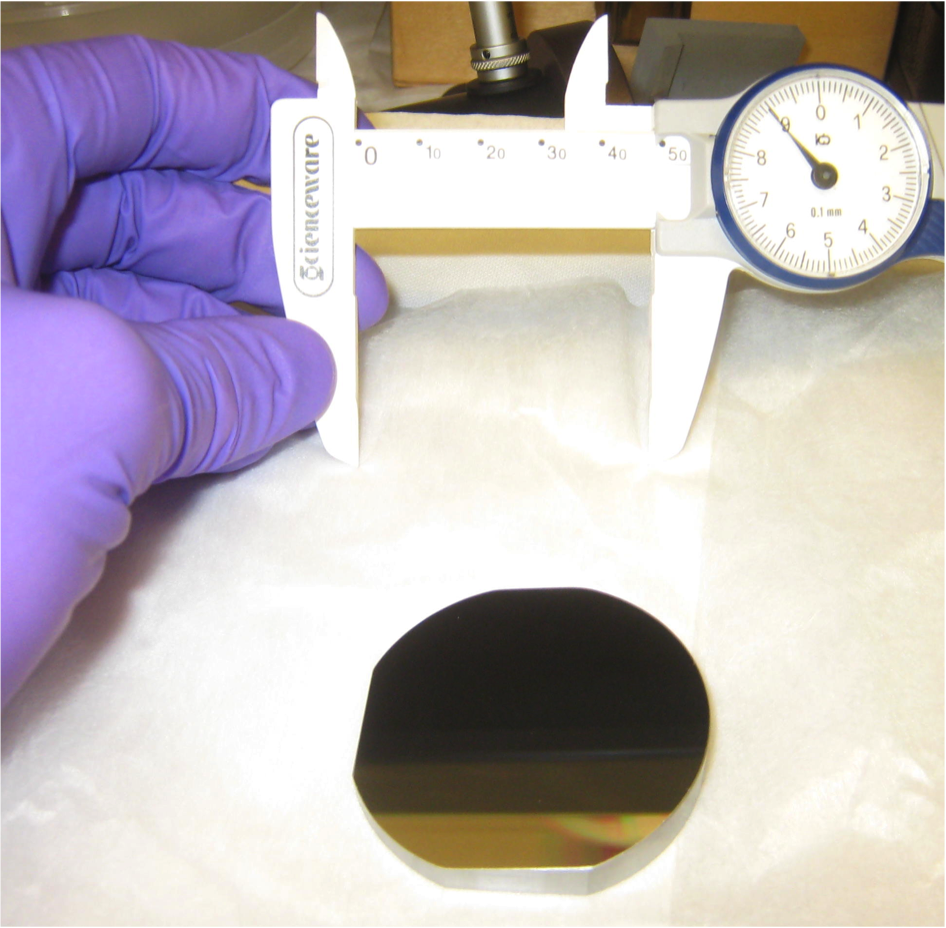
\includegraphics[height=9cm]{chSPIE_2010_JWST/figs/A6K_scale.png}
   \end{tabular}
   \end{center}
   \caption[JWST grism [pictures] 
   { \label{fig:im1} 
Photograph of flight grism ``A6K" for JWST-NIRCam.  The outer diameter is 48 mm and the part has an optically usable diameter of 42 mm.  The forward-facing surface has grooves with a period of 15.36 $\mu$m.  The opposite surface has been polished optically flat.  The flats along the perimeter serve as mounting and orientation surfaces}
   \end{figure} 

\subsection{Surface Flatness}
Because the parts are physically larger than the optically active area, it was possible to polish the flat surfaces of the JWST grisms to very high accuracy.  The specification for the polishing vendor was that the surface be flat to $\lambda$/10 peak to valley at 633 nm.  At 3.7 $\mu$m, this specification corresponds to a flatness of ~$\lambda$/60.  The difference of 2.4 in the refractive indices inside and outside the grism imposes similar flatness criteria for a silicon transmission optic to those one would impose on a mirror.  The achieved flatness of the entrance faces (Figure 2) did not always meet this optical specification but, in all cases, was very much better than required for diffraction-limited performance and these faces do not contribute to loss of performance in either throughput or resolution.  


   \begin{figure}
   \begin{center}
   \begin{tabular}{c}
   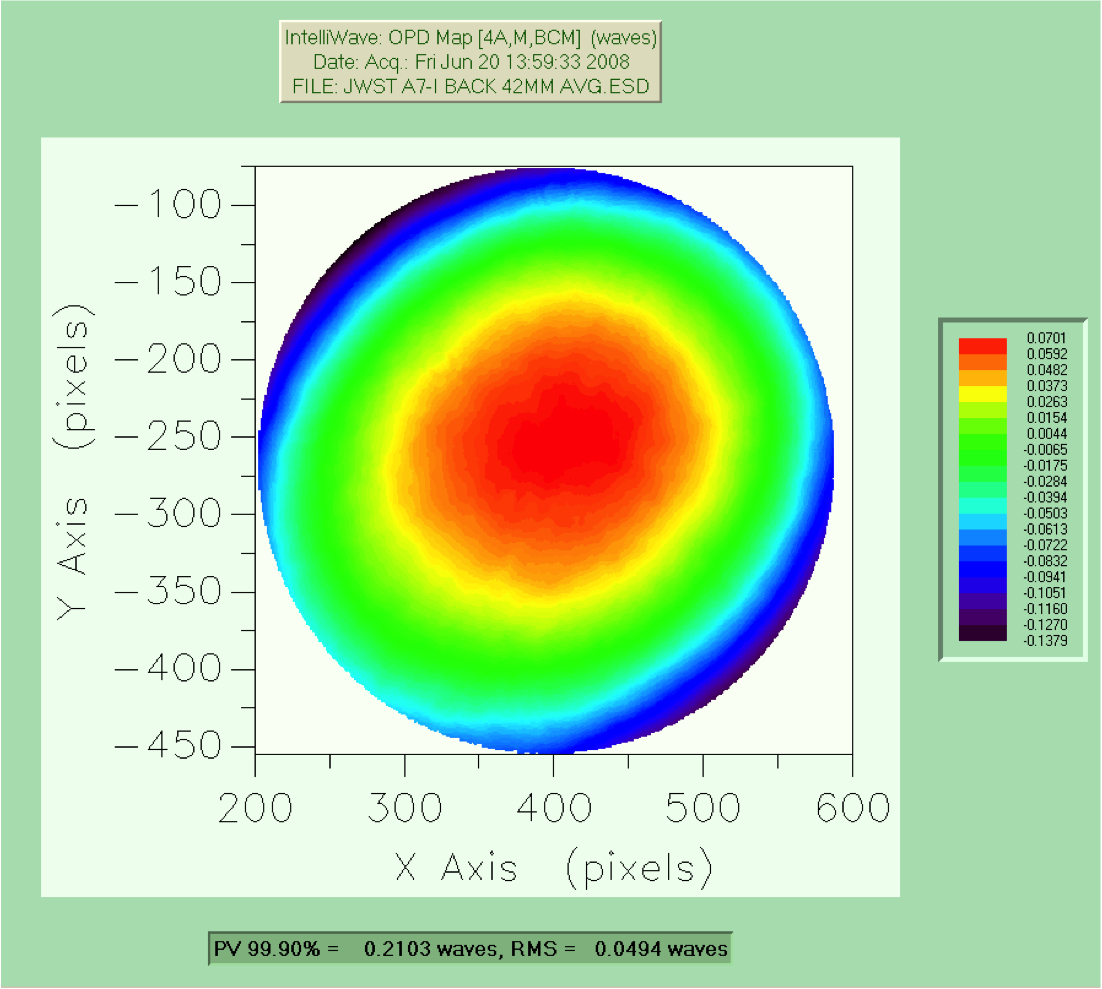
\includegraphics[height=7cm]{chSPIE_2010_JWST/figs/A7I_entrance_uncoat.png}
   \end{tabular}
   \end{center}
   \caption[A7-I interferogram] {\label{fig:im2}  Interferogram of the polished entrance surface of JWST trial grism ``A7-I".  The interferogram was taken prior to the application of an antireflection coating. }
   \end{figure} 

\subsection{Groove Geometry}
We form the grooves in the monolithic substrates from which we fabricate the grisms by taking advantage of the significantly different rates at which certain chemicals etch through the different planes in crystalline structure\cite{2007ApOpt..46.3400M,Tsang1975}.  In our process a solution of KOH etches approximately 60 times faster across the 100 plane than across the 111 plane and a suitably oriented mask of stripes will form triangular grooves at the intersection of 111 planes.  The intersecting planes form an angle of $71\,^{\circ}{\rm}$.  For blaze angles greater than $8\,^{\circ}{\rm}$, this acute angle will result in shadowing of one groove by another in transmission with the amount of shadowing a function of the blaze angle (see Figure 6 of Mar et al. (2006)\cite{Mar06}).  For small prism opening angles, it is not the acute groove vertex but rather the small dams along the grating surface that lead to groove filling factors less than one.  We need the dams to serve as etch stops between the grooves.  For the JWST gratings, the grating constant was 15.36 $\mu$m and the final dam width was about 1.5 $\mu$m.  At the $6.16 \,^{\circ}{\rm}$ opening angle of the JWST prisms, the dams are responsible for the filling factor loss.  The geometric blockage whether by the dams or by the lip of the neighboring acute groove leads to loss in two ways:  direct blockage of the light and, via Babinet's principle, diffraction of an equal amount of light into unwanted orders.  For the geometric blockage of $\sim10\%$ in the JWST grisms, the maximum theoretical transmission is then 0.81.  

\subsection{Microscopic Surface Roughness}
While the etching process results in remarkably flat grooves, point defects in the structure of the crystalline silicon grating substrates can lead to local pits and hillocks, that is, to roughness on various scales, as the anisotropic etching produces the blazed grooves.  The consequences of this roughness are difficult to measure directly as the scattered light produced as a result of it is generally on large angular scales with low peak amplitudes.  Instead, the best ways to evaluate this possible loss mechanism is to examine the roughness of the surfaces directly.  We have done this for an earlier set of grating surfaces using atomic force microscopy\cite{2007ApOpt..46.3400M} and concluded that the integrated diffuse scattered light due to small-scale roughness is 0.005\% for a Si grism in operation at 3.7$\mu$m.  We have also used interferometric metrology of roughness within individual grooves in the more demanding context of immersion grating production (see Wang et al. in this volume\cite{Wang10}) and find that the loss should be about 0.006\%  if such surfaces are used in transmission.


\subsection{Fresnel Losses}
The large refractive index ($\sim 3.41$ in the near-IR) that gives silicon grisms their large etendue also condemns them to substantial reflective (Fresnel) losses at the vacuum/Si interface.  For uncoated silicon, this loss is $\sim 30\%$ per surface.  When this loss is combined with the geometric loss, the maximum efficiency in the blaze order should be $\sim 0.41$.  Figure 3 shows the transmission versus wavelength curve for one of the NIRCam flight parts.  The tight delivery schedule for these parts did not allow us to measure the performance in first order, where the parts will be used in flight, but the on-blaze transmission of the uncoated gratings in modestly higher orders should be similar.  The peak transmission in 3$^{rd}$ order is 43\%, consistent to within the errors with the theoretical maximum. Even without an antireflection coating, the transmission of this grism is within the low end of the range of published efficiencies for near-IR grisms made from other materials and currently in use at ground-based telescopes, for example NSFCAM's KRS5 grism\cite{Rayner98} demonstrated  efficiencies of 55\%, 50\%, 40\% in orders 2, 3, and 4 which correspond to roughly the L, K, and H near-IR atmospheric bands.  

%Figure 3
   \begin{figure}
   \begin{center}
   \begin{tabular}{c}
   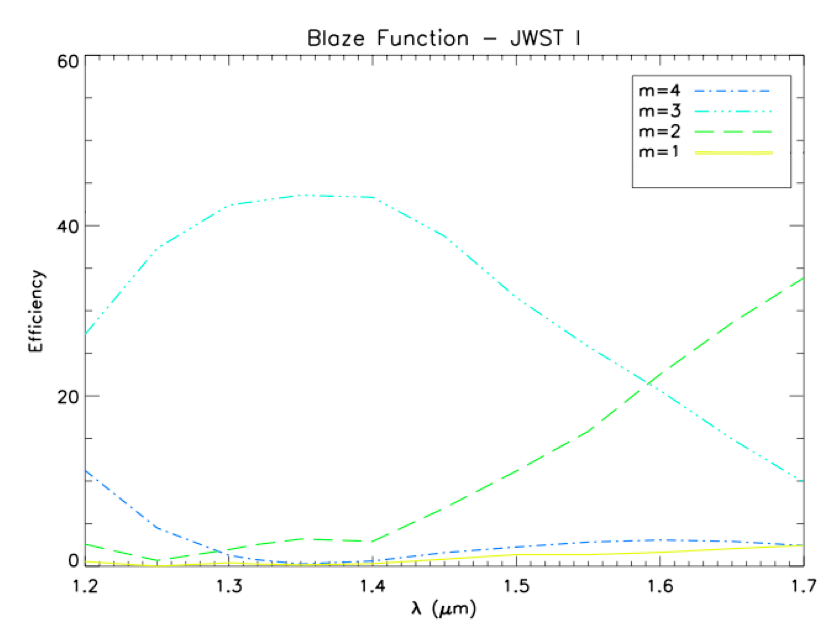
\includegraphics[height=9cm]{chSPIE_2010_JWST/figs/A6I_transmission_nt2}
   \end{tabular}
   \end{center}
   \caption[JWST grism transmission] {\label{fig:im3}  Measurement of throughput as a function of wavelength for JWST flight part ``A6-I".  The combination of the geometric blockage by the groove dams and the Fresnel losses results in a theoretical maximum efficiency of $\sim 0.41$ on the blaze.  The plot shows the power in the fifth order and in adjacent orders.} 
   \end{figure} 

\section{Results of Anti-Reflection Coating}
The initial plan for the JWST grisms was to coat only the flat side of each grism with a broad-band antireflection (AR) coating.  An ideal coating on this single face would result in a transmission of 0.57, a performance at the high end of the range of throughputs cited for grisms currently in use.  Figure 4 shows the transmission of a thin silicon wafer witness with an AR coating applied to one air-Si interface.  In the range of 2-5 $\mu$m, the transmission curve is consistent with Fresnel losses from only the uncoated surface, or in other words the AR coating transmits almost 100\% of the incident light.  

In a diffraction limited system, however,  one needs to be concerned about whether the process control for a multilayer coating is sufficiently good to preserve the observed flatness of the entrance face.  We were able to take interferograms of a geometrically similar test piece before and after a broad-band 2-5 $\mu$m antirection coating was applied.  The large-scale phase coherence won in the polishing of this surface has not been degraded by the addition of the multi-layer dielectric AR coating.
   
   %Figure 4
   \begin{figure}
   \begin{center}
   \begin{tabular}{c}
   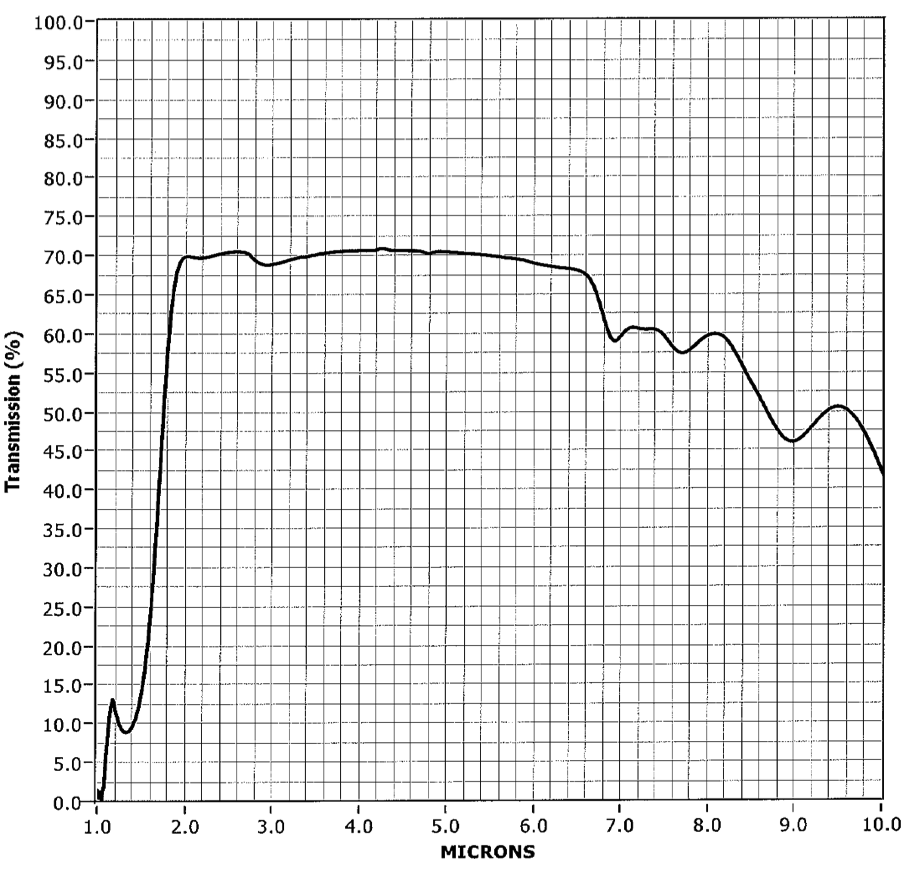
\includegraphics[height=10cm]{chSPIE_2010_JWST/figs/ARcoat_trans_siww}
   \end{tabular}
   \end{center}
   \caption[Transmission of single side AR coated silicon wafer witness] {\label{fig:im4}  IR transmission of an optically flat thin silicon wafer witness that was AR coated on a single side.  The wafer does not have grooves on it, and therefore does not have geometric losses.  Since the uncoated air-Si interface suffers 30\% Fresnel loss, the AR coated interface must exhibit close to 100\% transmission between 2 and 5 $\mu$m.  The AR coating is ineffective shortward of 2 $\mu$m, and Si does not transmit short of 1.15$\mu$m.  Figure courtesy of II-VI Inc.} 
   \end{figure} 
 
The only way to improve the delivered throughput beyond that achieved with the single-side coating would be to coat the grism grooves as well with a broad-band AR coating.  Such a procedure faces three potential problems:  (1) The shape of the groove makes it hard to deposit even layers of controlled thickness that are the basis for the efficacy of any antireflection coating. (2) Even small-amplitude variations in the summed thickness of the coatings could diminish the superlative phase coherence of the grating on large scales. (3) Even if the coating preserves coherence on large scales, variations in the deposition thickness within each groove could produce a change in the blaze shape from perfectly flat to structured in a way that might divert power out of the blaze order.

In the course of the development work for the JWST grisms, we were able to test the viability of AR coatings on the grating grooves by putting test coatings onto a prototype.  This prototype ``trial'' part (``A7-I") had the same groove constant and same vertex angle as the flight parts and flight spares but has an $11\,^{\circ}{\rm}$ blaze angle, rather than the $5.75\,^{\circ}{\rm}$ angle shared by the other parts.  The trial part functions well in the mid-infrared but differs from the flight parts in having its second-order rather than first-order blaze peak at the center of the band for the JWST long wavelength camera.  The difference in the prism opening angle and groove blaze angle means that the wavelength at the peak of the blaze is not undeviated as it is for the flight parts.  We coated this part with the same antireflection coating used for the flat surfaces of the flight parts, coating it first on the flat side and then, after measurement, on the grooved surfaces as well.  Throughput measurements were carried out by our group at UT Austin with a scanning monochromator or by II-VI Infrared Inc with their spectrophotometer.  The UT measurements were performed by measuring the ratio of the transmitted signal strength at the appropriate angle for the second-order beam to the signal from the monochromator incident on the detector with no intervening dispersive element.

%Figure 5: a) Transmission of uncoated trial part
                 %b) Transmission of coated trial part
   \begin{figure}
   \begin{minipage}[b]{0.5\linewidth} % A minipage that covers half the page
   \begin{tabular}{c}
   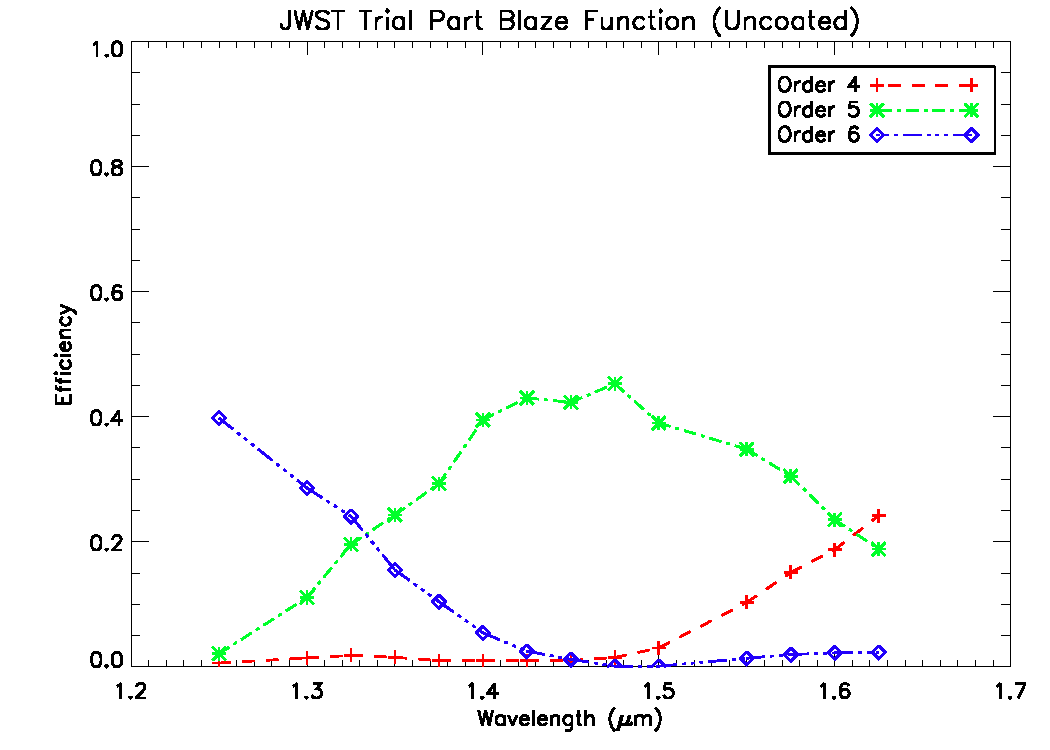
\includegraphics[width=\textwidth]{chSPIE_2010_JWST/figs/A7I_uncoated_trans.pdf}
   \end{tabular}
   \end{minipage}
   \hspace{0.01cm} % To get a little bit of space between the figures
\begin{minipage}[b]{0.5\linewidth}
   \begin{tabular}{c}
   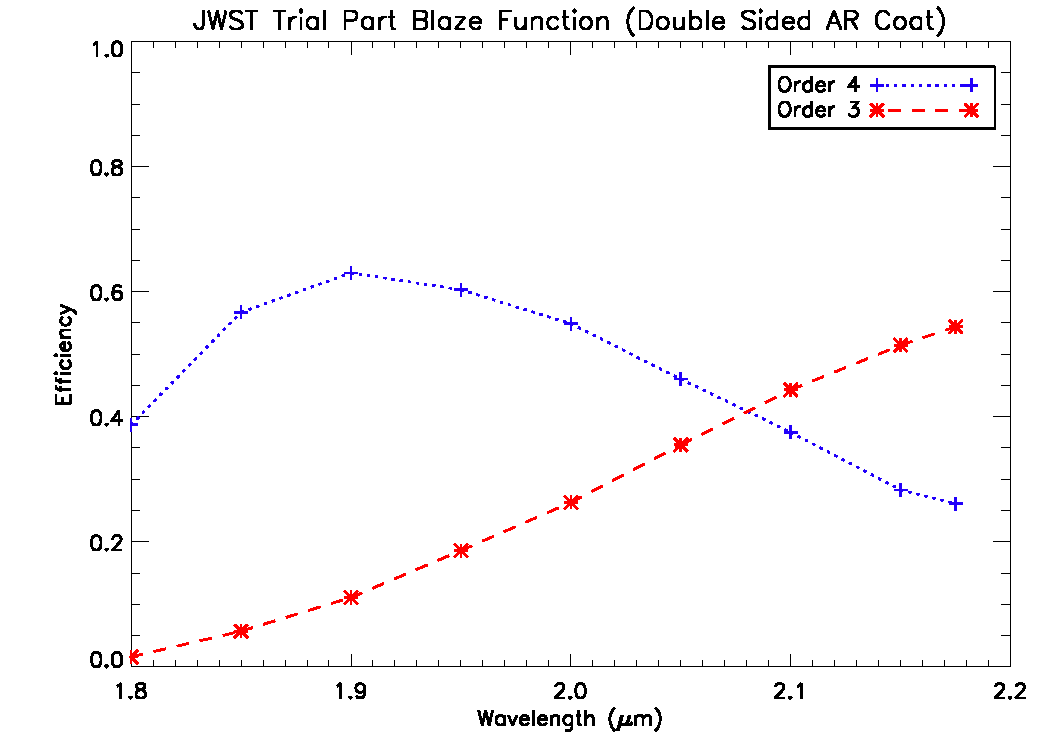
\includegraphics[width=\textwidth]{chSPIE_2010_JWST/figs/A7I_coated_2.pdf}
   \end{tabular}
   \end{minipage}
   \caption[JWST grism transmission] {\label{fig:im5}  Transmission of trial part A7-I.  The interferograms were taken with the surfaces (left) uncoated and (right) coated on both entrance and grating surfaces.  The ineffectiveness of the AR coating shortward of 2.0 $\mu$m (cf. Figure 4) stifled a direct comparison of transmission at the same wavelengths before and after coating.  The poor transmission below 2.0 $\mu$m is apparent in the right panel, since the $4^{th}$ order curve is suppressed before it reaches its blaze peak near 1.8 $\mu$m.  A similar measurement at 3.1-4.0 $\mu$m shows 75\% peak efficiency for the double-side coated grism.}
   \end{figure} 

The left panel of Figure 5 shows the performance of this part prior to the application of the coating while the right panel shows the transmission after A7-I had been AR coated on both its entrance and exit surfaces.  The right panel of Figure 5 does not reveal the peak on-blaze efficiency for two reasons- (1) the narrow wavelength range can only capture the $4^{th}$ order blaze peak and (2) the AR coating is ineffective at wavelengths shorter than 2.0 $\mu$m, suppressing the peak near 1.8 $\mu$m.  A coarse estimate for the blaze efficiency can be obtained by summing the power in orders 3 and 4 at a given wavelength, yielding an expected value for the peak efficiency of 80\%, which would be consistent with the maximum 81\% permitted by geometrical losses.  Our group has also performed throughput measurements from 3.1 to 4.0 $\mu$m that indicate 75\% efficiency at the $2^{nd}$ order blaze peak at 3.7 $\mu$m (see figure in C. Deen et al. in preparation).  The measurements at $2^{nd}$ order also indicate negligible power in the adjacent orders at 3.7 $\mu$m.  This observation is important because it means power was not diverted out of the blaze order after the AR coating was applied.  The multi-layer coating must not have altered the shape of individual grooves- variations in the deposition thickness within each groove must be very small.  This claim is also weakly supported by pre- and post- coating optical reflection measurements, which show similar ratios of power in the first and second brightest orders at 633 nm.  

Figure 6 shows a comparison of the 633 nm Littrow interferogram of the grooved surface of the trial part before (left) and after (right) the application of the antireflection coating.  While the images themselves appear quite dissimilar, the numbers at the bottom of the plot tell the true story.  The peak to valley deviation in the reflected phase front is virtually identical in the two cases and is extremely small ($< \lambda/100$ at the blaze wavelength). 



%Figure 6: a) Interferometry of uncoated trial part 31mm
                 %b) Interferometry of coated trial part 31mm
   \begin{figure}
   \begin{minipage}[b]{0.5\linewidth} % A minipage that covers half the page
   \begin{center}
   \begin{tabular}{c}
   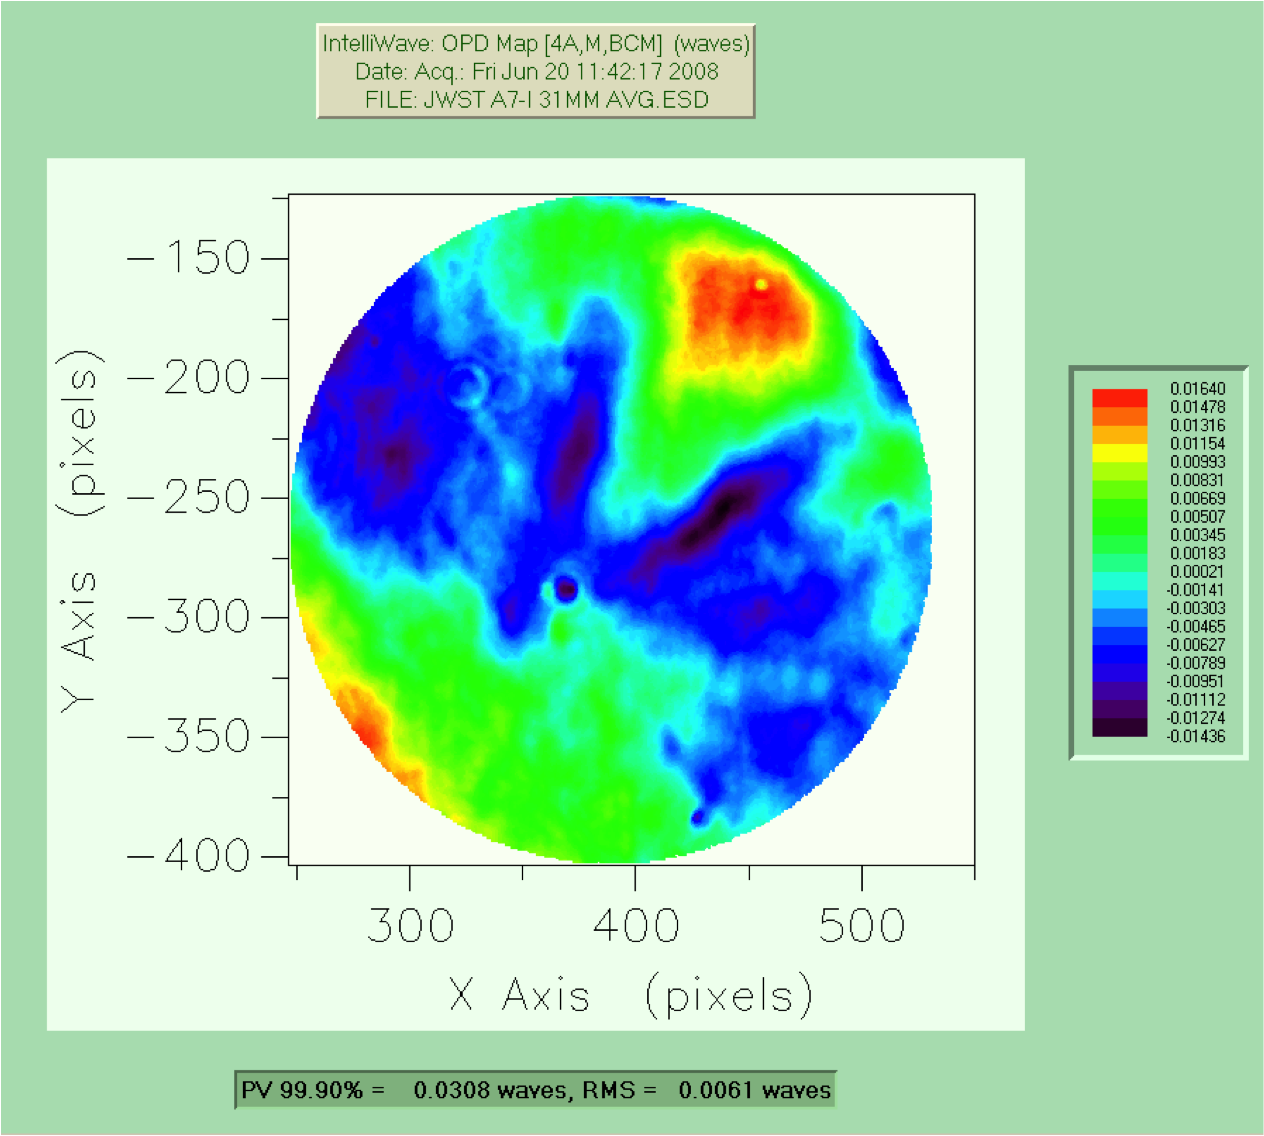
\includegraphics[width=\textwidth]{chSPIE_2010_JWST/figs/A7I_interf_31mm_grat_uncoat.png}
   \end{tabular}
   \end{center}
   \end{minipage}
   \hspace{0.0001cm} % To get a little bit of space between the figures
\begin{minipage}[b]{0.5\linewidth}
\begin{center}
   \begin{tabular}{c}
   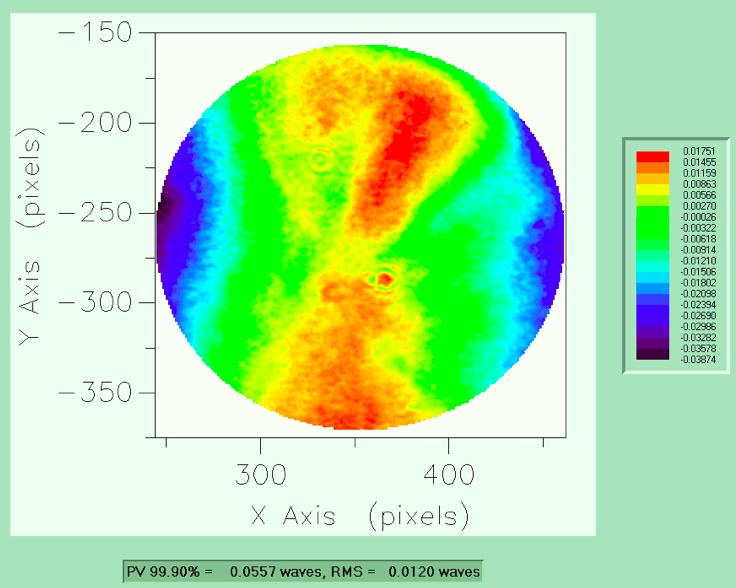
\includegraphics[width=\textwidth]{chSPIE_2010_JWST/figs/A7I_post_coat.png}
   \end{tabular}
   \end{center}
   \end{minipage}
   \caption[Trial part groove interferogram] {\label{fig:im6}  Optical interferograms at 633nm of the central 31 mm of the grooved surfaces of the trial part, A7-I.  The left figure shows the grooved surface before AR coating.  On the right is the interferogram of the grating surface after AR coating.  The RMS and peak to valley wavefront errors are printed at the bottom of the figures- \em{before}\em: PV- 0.0308, RMS- 0.0061 waves; \em{after}\em: PV- 0.0557, RMS- 0.0120 waves.}
   \end{figure} 


\section{Conclusions}
In summary, we have completed a set of six high performance silicon grisms for the NIRCam instrument on JWST.  The grisms are produced with precision photolithography and anisotropically etching the Si crystal plane.  By enumerating the loss mechanisms we saw that geometric and Fresnel losses limit the throughput of silicon grisms to about 41\%.  When the entrance and grating surfaces are coated with a broad band anti-reflection coating, Fresnel losses become negligibly small.  Measurements of a sample double side AR coated grism indicate on blaze throughput of about 75\%, marginally below the 81\% expected for purely geometric losses.  The grating performance was not significantly degraded by the multi-layer dielectric coating, as evinced by interferometry and optical reflection efficiency measurements.

\chapter{Near infrared metrology of high performance silicon immersion gratings} 



\section{Introduction}
\label{sec:intro} 

Immersion gratings are diffraction gratings illuminated within a high refractive index optical material, which provides increased spectral resolving power compared to diffraction gratings of comparable size illuminated in air or vacuum.  Scientific demands for high spectral resolving power combined with engineering demands for compact spectrographs make immersion gratings an attractive technology.  This report chronicles the lab performance of CA1a, an immersion grating made of silicon ($n_{Si}\sim3.4$).  CA1a or its spare CA1b will serve as the primary dispersive optical element for the Immersion Grating Infrared Spectrometer, IGRINS\cite{2010SPIE.7735E..54Y}.  We have reported on immersion grating design and fabrication elsewhere\cite{2007ApOpt..46.3400M}.  Wang et al. 2010\cite{2010SPIE.7739E.146W} reported on the science requirements for, fabrication of, and optical testing results of CA1, the parent Si boule puck from which CA1a was cut.  Since 2010 we have cut and polished two optical devices from CA1, and report here on their performance \emph{in immersion}.

%%%%%%%%%%%%%%%%%%%%%%%%%%%%%%%%%%%%%%%%%%%%%%%%%%%%%%%%%%%%%
\section{Overview} 
Figure \ref{fig:CA1aphoto} shows a photo of the final immersion grating CA1a after cutting, polishing, AR coating, and aluminization.  The trapezoidal side profile is a relic from the shape of the parent substrate and our cutting strategy.  The optically active volume is the prism shown above the dashed line in the photo in Figure \ref{fig:CA1aphoto}.  We left on additional silicon to strengthen the thin end of the prism wedge.  The front entrance face has a multi-layer dielectric anti-reflection (AR) coating, which, based on direct measurements off the CA1a entrance face, has a reflectivity  $<1\%$ across the 1.4$-$2.5 $\mu$m range.  The grating grooves were aluminized with a conformal Al layer.  Cryogenic testing of heritage gratings demonstrated that the conformal layer of Al is robust to typical cryogenic thermal cycling\cite{2007ApOpt..46.3400M}. We have not yet cooled CA1a.

\begin{figure}
  \centering
  \subfloat[CA1a photo]{\label{fig:CA1aphoto}\includegraphics[height=5cm]{chSPIE_2012_CA1/figs/ca1_bartest2}}
	~
%  \subfloat[CA1a drawing]{\label{fig:CA1adraw}\includegraphics[page=1, trim=24cm 15.15cm 2cm 5cm, clip=true, totalheight=0.2\textheight ]{APRA_BOULE_29MM_R3_CA1_X14_2011-03-08}}
   \subfloat[CA1a drawing]{\label{fig:CA1adraw}\includegraphics[height=4cm]{chSPIE_2012_CA1/figs/ca1a_drawing}}
  \caption[Photo and design drawing of the IGRINS immersion grating]{Photo and design drawing of the immersion grating CA1a in the lab in August 2011.  The entrance face is on the right, with a light green color in the photo (color available in the digital manuscript), which is due to the AR coating.  The grating surface is on the top with microscopic grating lines perpendicular to the long edge of the grating.  In operation a 25 mm circular beam will be incident on the entrance face and will project into an ellipse on the grating surface as seen in the drawing.  The dispersed light will reemerge from the entrance face.  The units in the drawing are mm.  The parent substrate and grating geometry are pictured in Figures 1, 3, and 4 in Wang et al. 2010\cite{2010SPIE.7739E.146W}.  Those figures reveal how the CA1a trapezoid shape and curved rear edge derive from the parent substrate shape.}
  \label{fig:gram}
\end{figure}

\begin{table}[h]
\caption {CA1 grating and substrate properties} \label{tab:title} 
\begin{center}
\begin{tabular}{lc}
\hline
Property & Value \\
\hline
Pitch, $\sigma$ ($\mu$m)  & 27.36 \\
$\;\;\;\;\;\;\;\;\;\;\;\;$(l/mm) & 36.55\\
Groove top, $t$ ($\mu$m)  & 9.95 \\
Blaze angle, $\delta$ ($^\circ$)  & 71.6$\pm$0.2 \\
Apex angle, $A$ ($^\circ$) & 72.1$\pm$0.2 \\
\multicolumn{2}{c}{\emph{Material properties}} \\
Material & High resistivity float zone Si \\
Average Refractive index & 3.44 \\
Specific heat ($J g^{-1} K^{-1}$) & 0.71 \\ 
\hline
\end{tabular}
\end{center}
\end{table}


We produce the grating grooves by photolithography and anisotropic chemical wet etching\cite{2007ApOpt..46.3400M,2010SPIE.7739E.146W}.  This process has some special features.  The wet etching process makes acute angle grooves, not 90$^\circ$ grooves, as illustrated in Figure \ref{fig:CA1aSEM}.  The groove apex angle $A=70.5^\circ$ is the intersection of two 111 Si crystal planes.  We anticipated an apex angle widened by 0.8$^\circ$ on both sides, for a net apex angle of about $A=72.1^\circ$.  A finite but small amount of etching accross the 111 crystal planes causes the small 0.8$^\circ$ angular correction\cite[Figure 5]{2007ApOpt..46.3400M}.  The anisotropic correction similarly decreases the blaze angle $\delta$ by $\Delta \delta = 0.8^\circ$.  This effect must be accounted for, first at the time of the initial x-ray orientation and cutting of the parent substrate and second at the time of cutting the immersion prism from the Si parent substrate.  We verified the delivered blaze angle after wet etching but before cutting our immersion grating prism by measuring the relative intensity of eight diffracted orders in reflection in air at the air-Si grating interface.  We made a simple scalar diffraction theory model and compared it to the observed intensity of the eight orders surrounding order 82, the brightest observed order at 632.8 nm in front-surface reflection.  The measurements were performed in the Littrow configuration.  The model predicted the effect of the blaze envelope as a function of incidence angle.  We found $\delta=71.63\pm0.20^\circ$, consistent within the uncertainty with $\delta = R3$, so we cut the front face to R3.  The apex and blaze angles are conspicuous in the SEM cross section (Figure \ref{fig:CA1aSEM}).  Importantly, the groove apex shows a sharp peaked tip with no evidence of a flat bottom, which can occur in incomplete wet etching.  Flat bottoms cause a direct efficiency loss by diffracting light away from the blaze.  In the right panel of Figure \ref{fig:CA1aSEM} the optically active facets are highlighted.  The flat groove tops on the grating surface are artifacts of the groove formation process.  Specifically, nitride coated groove tops serve as anisotropic wet etch dams.  It is clear from the annotated SEM micrograph that the groove tops are shadowed for light incident at or close to the blaze angle.  The groove tops will be shadowed so long as the ratio of the grating top $t$ to pitch $\sigma$ ratio satisfies the condition:
\[ 
\frac{t}{\sigma} < \frac{1}{1+\frac{ \tan (A) }{ \tan (\delta{}) }}, 
 \] 
For our grating, $t/\sigma=0.36<0.49$, so the optically active groove facets fully shadow the groove tops as planned.  The SEM micrographs are not sensitive enough to small ($\sim5$ nm) scale groove position errors, so detailed optical and IR metrology is necessary to evaluate the performance.

%-------------
   \begin{figure}
   \begin{center}
   \begin{tabular}{c}
   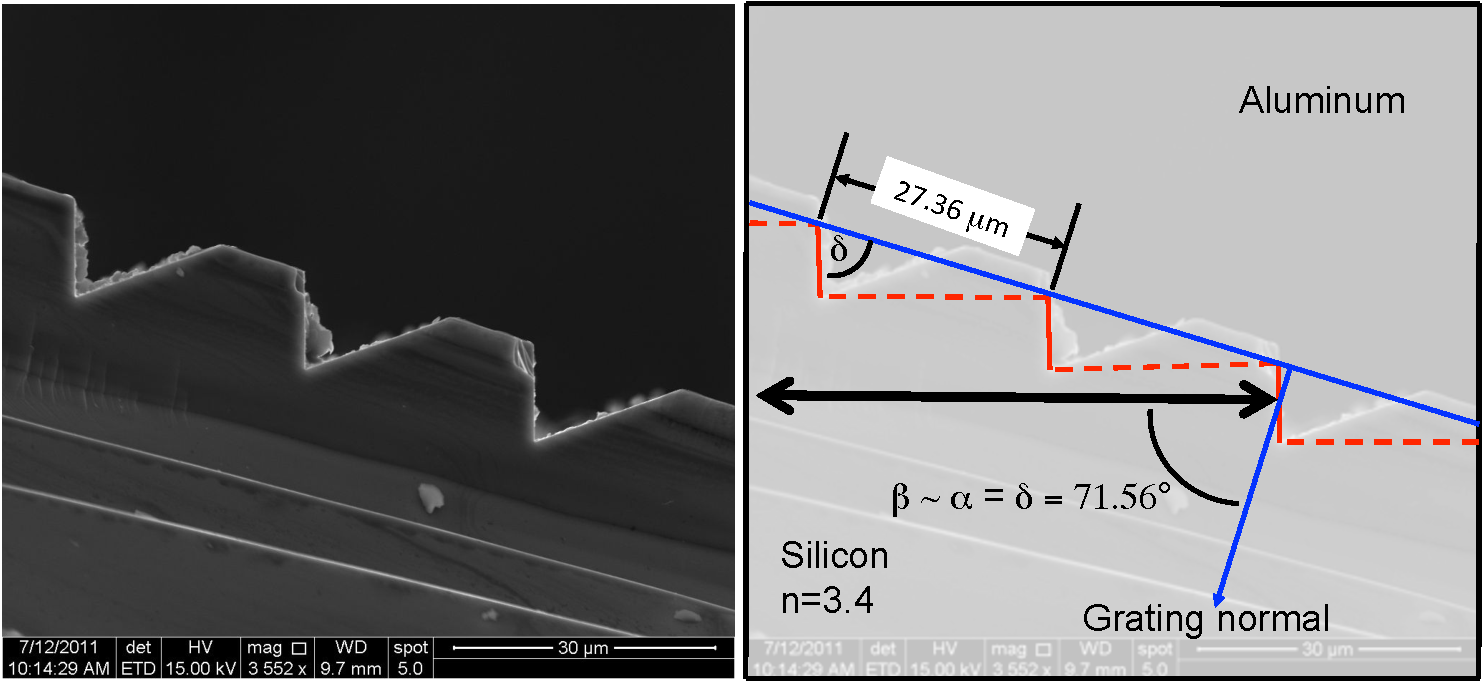
\includegraphics[height=7cm]{chSPIE_2012_CA1/figs/CA1_SEM_cross3}
   \end{tabular}
   \end{center}
   \caption[CA1a SEM]{ \label{fig:CA1aSEM}  Scanning electron micrograph (SEM) of a $\sim$100 $\mu$m cross section of a scrap portion of the immersion grating CA1.  The left panel is the unaltered SEM.  The right panel is a schematic illustrating the grating specifications and the geometry of incident and diffracted beams (thick black line with arrows).  The beam is incident from the left, and diffracts at the facets at the silicon/aluminum interface.  The incident angle $\alpha$ and diffracted beam $\beta$ are measured from the grating normal (shown in blue).  The blaze angle $\delta$ is set by the orientation of the crystal planes with respect to the grating surface.  This angle was designed to be $\delta=71.56^\circ$, which is the angle whose tangent is 3.  The optically active facets are highlighted as short red vertical lines (\emph{color online}).  The regions of the grating above the dashed line do not see the beam.  In the IGRINS design and in our lab testing there is a small out of plane angle $\gamma$ not shown here.  The apparent hillock artifacts on the grating facets are a result of the cross-section preparation process, the measured\cite{2010SPIE.7739E.146W} surface flatness is 1.7 nm.}
   \end{figure} 
%-------------

\section{Efficiency} 
For optimal performance immersion gratings should be as efficient as possible.  The IGRINS specification for immersion grating efficiency is 65-70\% peak on blaze\cite{2010SPIE.7739E.146W}. We directly measured the AR-coated entrance face reflective loss at $<1\%$ over the measured range $1500-2300$ nm.  From measurements of the microscopic surface roughness\cite{2010SPIE.7739E.146W} we expect scattered light from microscopic surface roughness to be $<0.5\%$.  We directly measured the immersion grating efficiency as a function of wavelength with a custom scanning monochromator setup in our lab, described in the Section \ref{sec:GTA}.  The reference mirror was aluminum on glass, so the absolute grating efficiency is about 3.5\% lower than reported here, assuming aluminum reflectance of 95\% in the near-IR.  Recall that the grating grooves are aluminized, so the reported relative efficiency is a good indicator of how well the bulk of the immersion grating is performing.  The measurement shown in figure \ref{fig:CA1a-efficiency} has 1 nm bandwidth, with 1nm sampling over the range $1500-2300$ nm.  The measured peak on-blaze efficiency is between 70\% and 80\% across all 43 orders, except for order 120 which has a peak efficiency of 68\%.  CA1a was measured with an out of plane angle \cite{schroeder1987}, $\gamma \sim 2.6^\circ$ in immersion.  We only coarsely controlled the incidence angle $\alpha$ in our efficiency measurement, with $\alpha \sim \delta$ to within about 2$^\circ$.  Accordingly, we measured some angularly dependent diffraction loss that one would expect if orders diffracted into the grating sidewalls.  It is best to have $\alpha > \delta$ so that the blaze envelope is centered at $\beta < \delta$.


\begin{figure}
\begin{center}
 \begin{tabular}{c}
    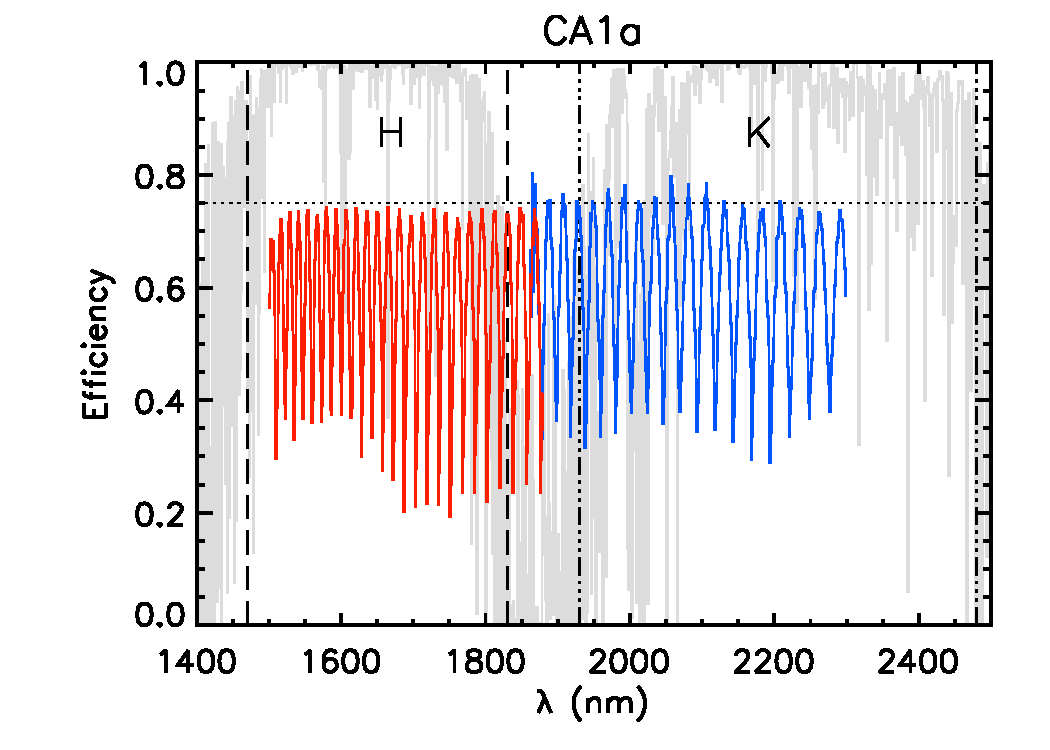
\includegraphics[width=1.0\textwidth]{chSPIE_2012_CA1/figs/CA1a_1500_2300_eff.pdf}
   \end{tabular}
  \end{center}
  \caption[CA1a Efficiency]{\label{fig:CA1a-efficiency} Efficiency of CA1a as a function of wavelength.  The measurements for 1500$-$2300 nm cover orders 120 to 78.  The peak on-blaze efficiency is typically about 75\% of an aluminum reference mirror, as shown by the horizontal dotted line at 75\%.  The vertical dashed lines at 1450 and 1900 nm demarcate the designed wavelength range of IGRINS $H-$band channel.  Similarly, the vertical dash triple-dotted lines demarcate the $K-$band channel.  The faint gray line in the background is the atmospheric transmission over Kitt Peak\cite{hinkle1995}.  Measurements at $\lambda > 2300 $ nm we not performed at the time of writing.  The slightly suppressed efficiency at 1500 nm may result from visible light leakage in the reference mirror measurement from our 1450 nm low pass filter operated in uncollimated light, or perhaps from real polarization sensitive effects.  See the notes on the next figure's caption regarding the difference in measurements shortward and longward of 1870 nm.}
\end{figure}

 There are a few potential loss mechanisms which lead to the observed efficiency:
\begin{enumerate}
\item Fresnel loss from entrance through the front vacuum/Si interface
\item Loss from microscopic groove and entrance face surface roughness that goes into scattered light
\item Loss at the Si/Al interface due to dielectric effects
\item Diffraction into other orders
\item Fresnel loss from exit through the front Si/vacuum interface
\item Systematic measurement error in beam alignment or collimation
\end{enumerate}

\section{Refractive index dependence}
The refractive index of silicon is wavelength and temperature dependent, so the blaze pattern in Figure \ref{fig:CA1a-efficiency} will be different at the cryogenic operating temperature of an IR spectrograph.  Precise measurements for crystalline Si are available for the CHARMS group at Goddard \cite{2006SPIE.6273E..77F}.  The right panel of figure \ref{fig:CA1a-diffrac} shows the refractive index as a function of wavelength for 296 K, 273 K, and 77K, using the Sellmeier equation from the Goddard group and assuming vacuum wavelengths.  The index goes from about 3.483 to 3.445 in the wavelength range 1.5 to 2.3 $\mu$m, which is a change of about 1\%.  The index decreases by an average of 0.8\% from room temperature to 77K.  The index intimately controls both the diffraction angle $\beta$ at the Si-Al grating interface via the grating equation, and the refraction angle $\theta$ at the Si-vacuum interface via Snell's law.  For example the wavelength $\lambda=2.290 \;\mu$m at room temperature is diffracted to 78th order near the peak of the blaze.  Reducing the temperature to 77K decreases the index of refraction by 0.8\%. This puts $\lambda= 2.290 \;\mu $m into 77th order, which is at the edge of the blaze.  The grating period $\sigma$ also shrinks by a factor of the coefficient of thermal expansion (CTE) of Si, $\alpha \sim 3\times10^{-6}/^\circ$C.  From room temperature to 77K the fractional shrinkage is about 0.06\%, which is an order of magnitude less than the effect of the index of refraction.  Furthermore, the CTE effect will have no effect at the Si-vacuum interface.

\begin{figure}
\begin{center}
 \begin{tabular}{c}
    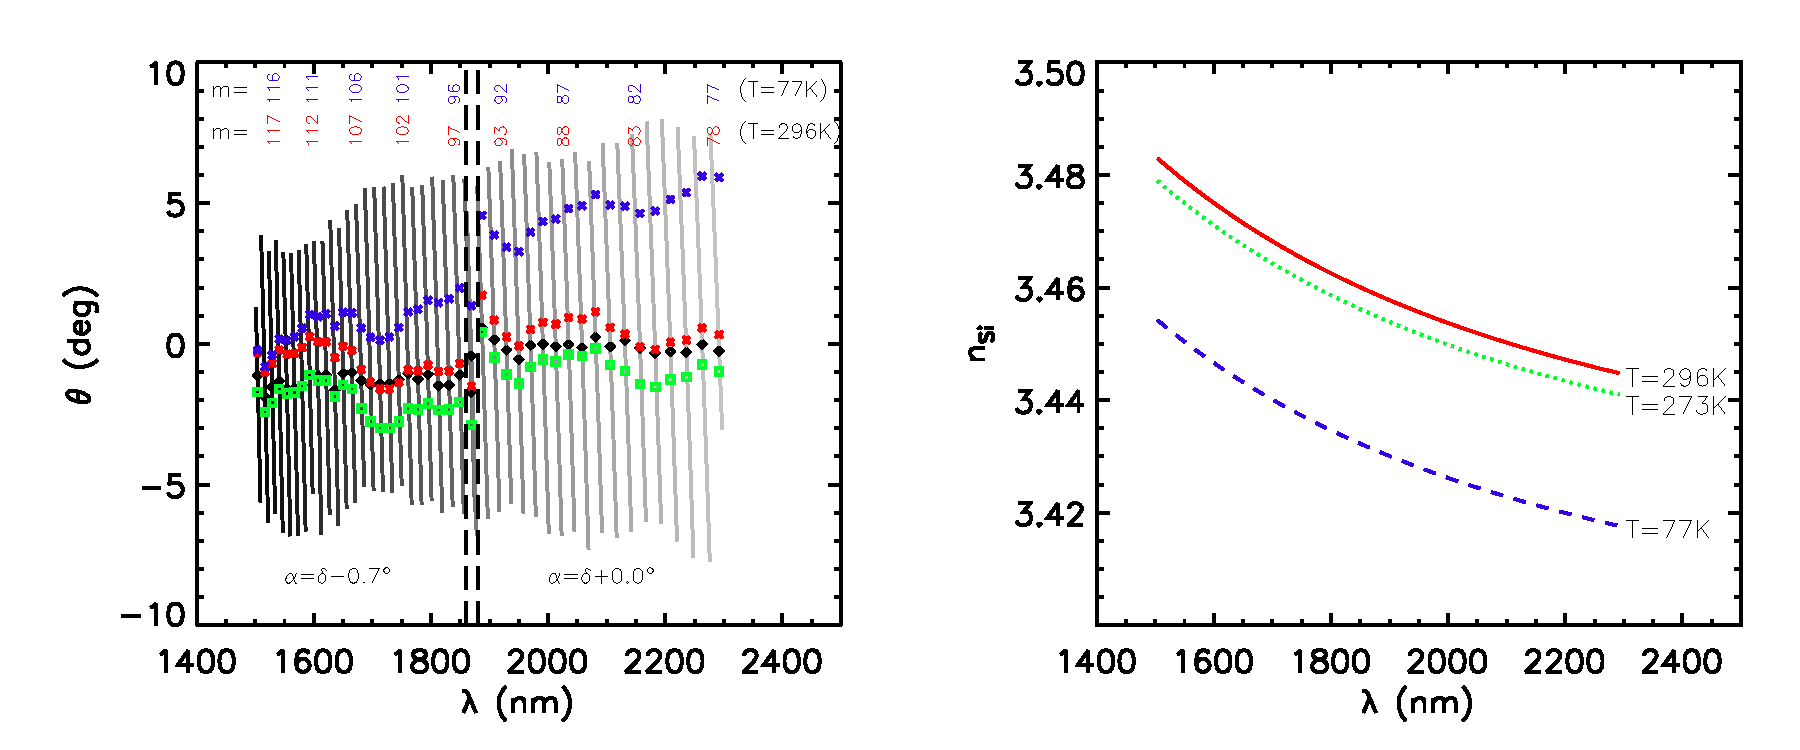
\includegraphics[width=1.0\textwidth]{chSPIE_2012_CA1/figs/CA1a_diffrac}
   \end{tabular}
  \end{center}
  \caption[CA1a Diffraction]{\label{fig:CA1a-diffrac} Measured and predicted diffraction angles for CA1a.  The right panel is the index of refraction as a function of wavelength \cite{2006SPIE.6273E..77F} for T = 296, 273, and 77 K.  The left panel is the angular position of diffracted beams as a function of wavelength.  The almost vertical lines are approximately 1 free spectral range of the observed 43 diffraction orders for $1500 < \lambda (\textrm{nm}) < 2300$ in air at T = 296K.  The order numbers for every fifth order, starting at 78th order are marked at the top.  The black diamonds are the observed peaks of the blaze efficiency (cf. figure \ref{fig:CA1a-efficiency}).  The measurements longward and shortward of $\lambda=1870$ nm have slightly different incidence $\alpha$ angles, which jogged the the blaze center positions.  The red $\ast$, green square, and blue $\times$ demarcate the expected positions of beams from scalar optics diffraction and refraction theory assuming a Si refractive index at the temperatures of T=296, 273, and 77 K, respectively.  The model corrects for $\alpha \neq \delta$ measurements for $\lambda < 1870 $ nm, causing a jog in the $\theta(\lambda)$ trend highlighted by the vertical black dashed lines.  The temperature change shifts the position of diffracted beams by an entire order.}
\end{figure}

\section{Periodic errors, ghosts, and large scale performance} 

\begin{figure}
  \centering
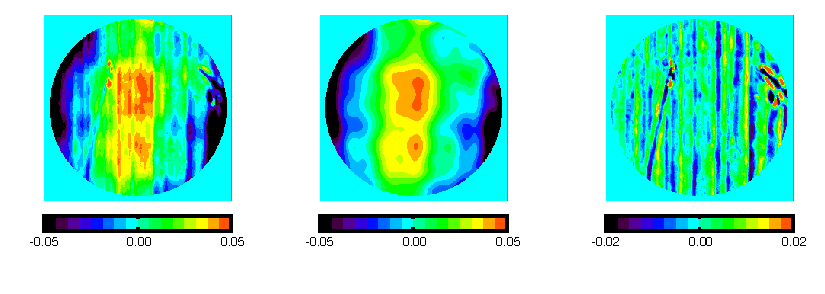
\includegraphics[width=0.9\textwidth]{chSPIE_2012_CA1/figs/CA1a_fig_scl2}
  \caption[Optical interferometry of the IGRINS immersion grating]{Optical interferometry of CA1a in reflection off the back surface before cutting and aluminization.  The color scales are in waves of surface error for 632 nm in reflection.  \emph{Left:} Interferogram measured in Littrow reflection at R3 over a 23.75 mm beam on the parent substrate CA1, in the vicinity where CA1a was later cut.  The colorbars show the vertical scale in waves of surface distortion at $\lambda = $ 632.8 nm.  These optical measurements illuminate the back of the grating facets, they were taken before aluminization and should be a good proxy for immersion performance at 2.15 $\mu$m. \emph{Center:} A fit to the large scale surface distortion using the first 200 Zernike polynomials in the Noll Sequence \cite{noll1976}.  \emph{Right:} The residual high spatial frequency surface error constructed from subtracting the fit from the measured surface error.}
  \label{fig:gram}
\end{figure}

Figure \ref{fig:gram} shows the optical 632 nm interferogram of CA1 in reflection in air.  The peak to valley surface error is 0.17 waves.  These interferograms should be equivalent to 2.16 $\mu$m in immersion in a cryogenic environment.  The shortest operational wavelength for the IGRINS instrument is 1.45 $\mu$m, at which the surface error is 0.25 waves.  The surface structure can be broken into two components, the large scale surface aberration and and a periodic error of parallel stripes parallel to the grating grooves.  Figure \ref{fig:gram} shows the large scale surface aberration in the middle panel and the periodic error on the right panel.  The vertical stripes are conspicuous in the right panel, while the center panel looks like a typical residual optical surface aberration possessing relatively low amplitude.  The main power in the periodic error is in a single sine wave with 5 mm deprojected period and amplitude of 3.2 nm.  There are other harmonic components with higher spatial frequency and comparable or lower amplitude.  

The origin of the large scale surface aberration is a combination of the dozen or so processing steps that go into delivering the final immersion grating.  Chief among these is the UV contact photolithography step.  The reactive ion etching, wet etching, and surface preparation steps may also contribute to the overall surface error.  The periodic stripes arise in the UV photolithography process that transfers the pattern from the photomask to the underlying photoresist.  Specifically the contacted mask and Si substrate pair repeatedly translate beneath a 1 cm wide UV slit to deliver the requisite UV dose.  We discovered that the translation stage had a periodic speed change which is equivalent to a periodic exposure time as a function of position on the photoresist.  Prototype gratings made since CA1 have corrected for this problem and surface errors attributable to periodic errors have largely disappeared.  

The major problem with periodic errors is that they cause symmetric ghosts surrounding the main diffraction peak.  The intensity of the ghosts relative to the main peak is related to the periodic error amplitude by\cite{2007ApOpt..46.3400M,james2007,2010SPIE.7739E.146W}:
\begin{eqnarray}
	\frac{I_{\textrm{ghost}}}{I_{\textrm{line}}}= \left \lbrack \frac{2\pi n}{\lambda} \xi \sin{\delta} \right \rbrack ^2
\end{eqnarray}
where $\xi$ is the amplitude of the spacing error.  Figure \ref{fig:PSFzygo} shows a logarithmically scaled PSF from optical interferometry of CA1a in reflection from the aluminized surface in air at 632.8 nm over a 25 mm circular aperture.  The measured intensity of the ghost relative to the main peak is $I_{g}/I_{0}=9\times10^{-4}$.  Optical spectral purity lab measurements at 632.8 nm are higher by 20\%.  Measurements at 543 nm (comparable to 1.87 $\mu$m in immersion), show a level of $I_{g}/I_{0}=1.6\times10^{-3}$, which is 30\% greater than one would expect from scaling interferometrically derived intensity at 632.8 nm.  Extrapolating the interferometrically derived intensity to 1.45 $\mu$m in immersion, the ghosts in IGRINS will have a peak intensity of 0.2\% of the main peak.  Quantitative lab measurements at 1.523 $\mu$m in immersion were attempted but were not reliable due to nonlinear response at the requisite high dynamic ranges need to measure the low ghost levels.  

\begin{figure}
\begin{center}
 \subfloat[2D Zygo PSF]{\label{fig:zygoPSF2D} 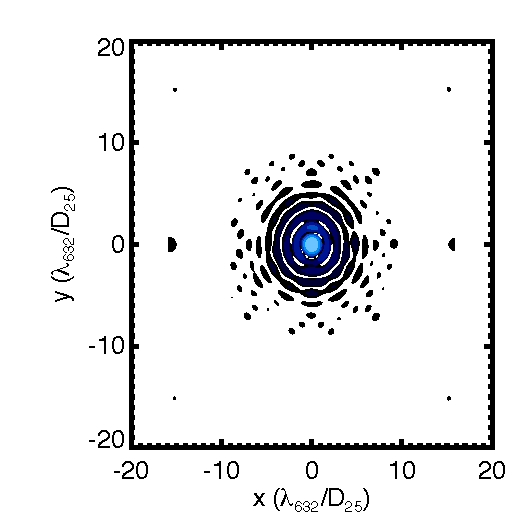
\includegraphics[width=0.45\textwidth]{chSPIE_2012_CA1/figs/CA1a_ghost_zygo_2d}}
 \subfloat[1D Log PSF]{\label{fig:logPSF1D} 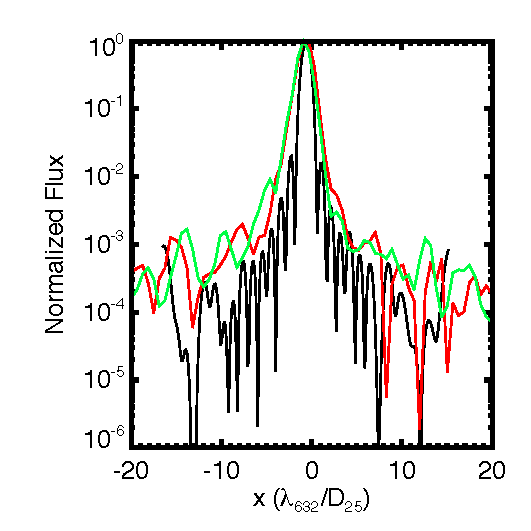
\includegraphics[width=0.45\textwidth]{chSPIE_2012_CA1/figs/CA1a_ghost_1d}}   
  \end{center}
  \caption[Immersion grating interferogram PSF]{\label{fig:PSFzygo}  Left: The 2-dimensional synthetic PSF from interferometric measurements of the air-aluminum reflective interface of CA1a at 632.8 nm at R3.  The dispersion direction is $x$, the cross-dispersion or spatial dimension is $y$.  The units on the axes are in terms of diffraction widths of $\lambda=$ 632.8 nm and $D=$ 25 mm, which were the conditions of the interferometry.  The scale on the 2D image is linear, compare to the intensity levels shown on the right panel.  Right:  The 1D logarithmically scaled horizontal line profile of the PSF of CA1a under three conditions.  The black is the synthetic interferometric PSF.  The red is the lab-measured PSF in reflection at 632 nm with a 20 mm beam.  This measurement is not diffraction limited.  The green line is the measurement at 543 nm in reflection with a 20 mm beam.}
\end{figure}


\section{Measurement setup description} \label{sec:GTA}
The basic strategy of the custom efficiency measurement setup is to compare the chopped signal from the immersion grating to an aluminum mirror.  The monochromator outputs 1 nm bandwidth and we sample at 1 nm steps.  The basic layout is a light source, 1.45 $\mu$m long pass filter, Spectral Products DK480 scanning monochromator, a chopper, collimating and relay optics, a motorized swing arm, a single pixel PbS array, and a lock-in amplifier.  The DK480, motorized swing arm, and lock-in amplifier are all computer controlled.  Custom software predicts the diffraction angles of the immersion grating and fine scans the swing arm around the predicted angular order positions.  Figure \ref{fig:GTAview} shows a labelled photo of the measurement apparatus, with detailed description of the optical path in the figure caption.  

\begin{figure}
\begin{center}
    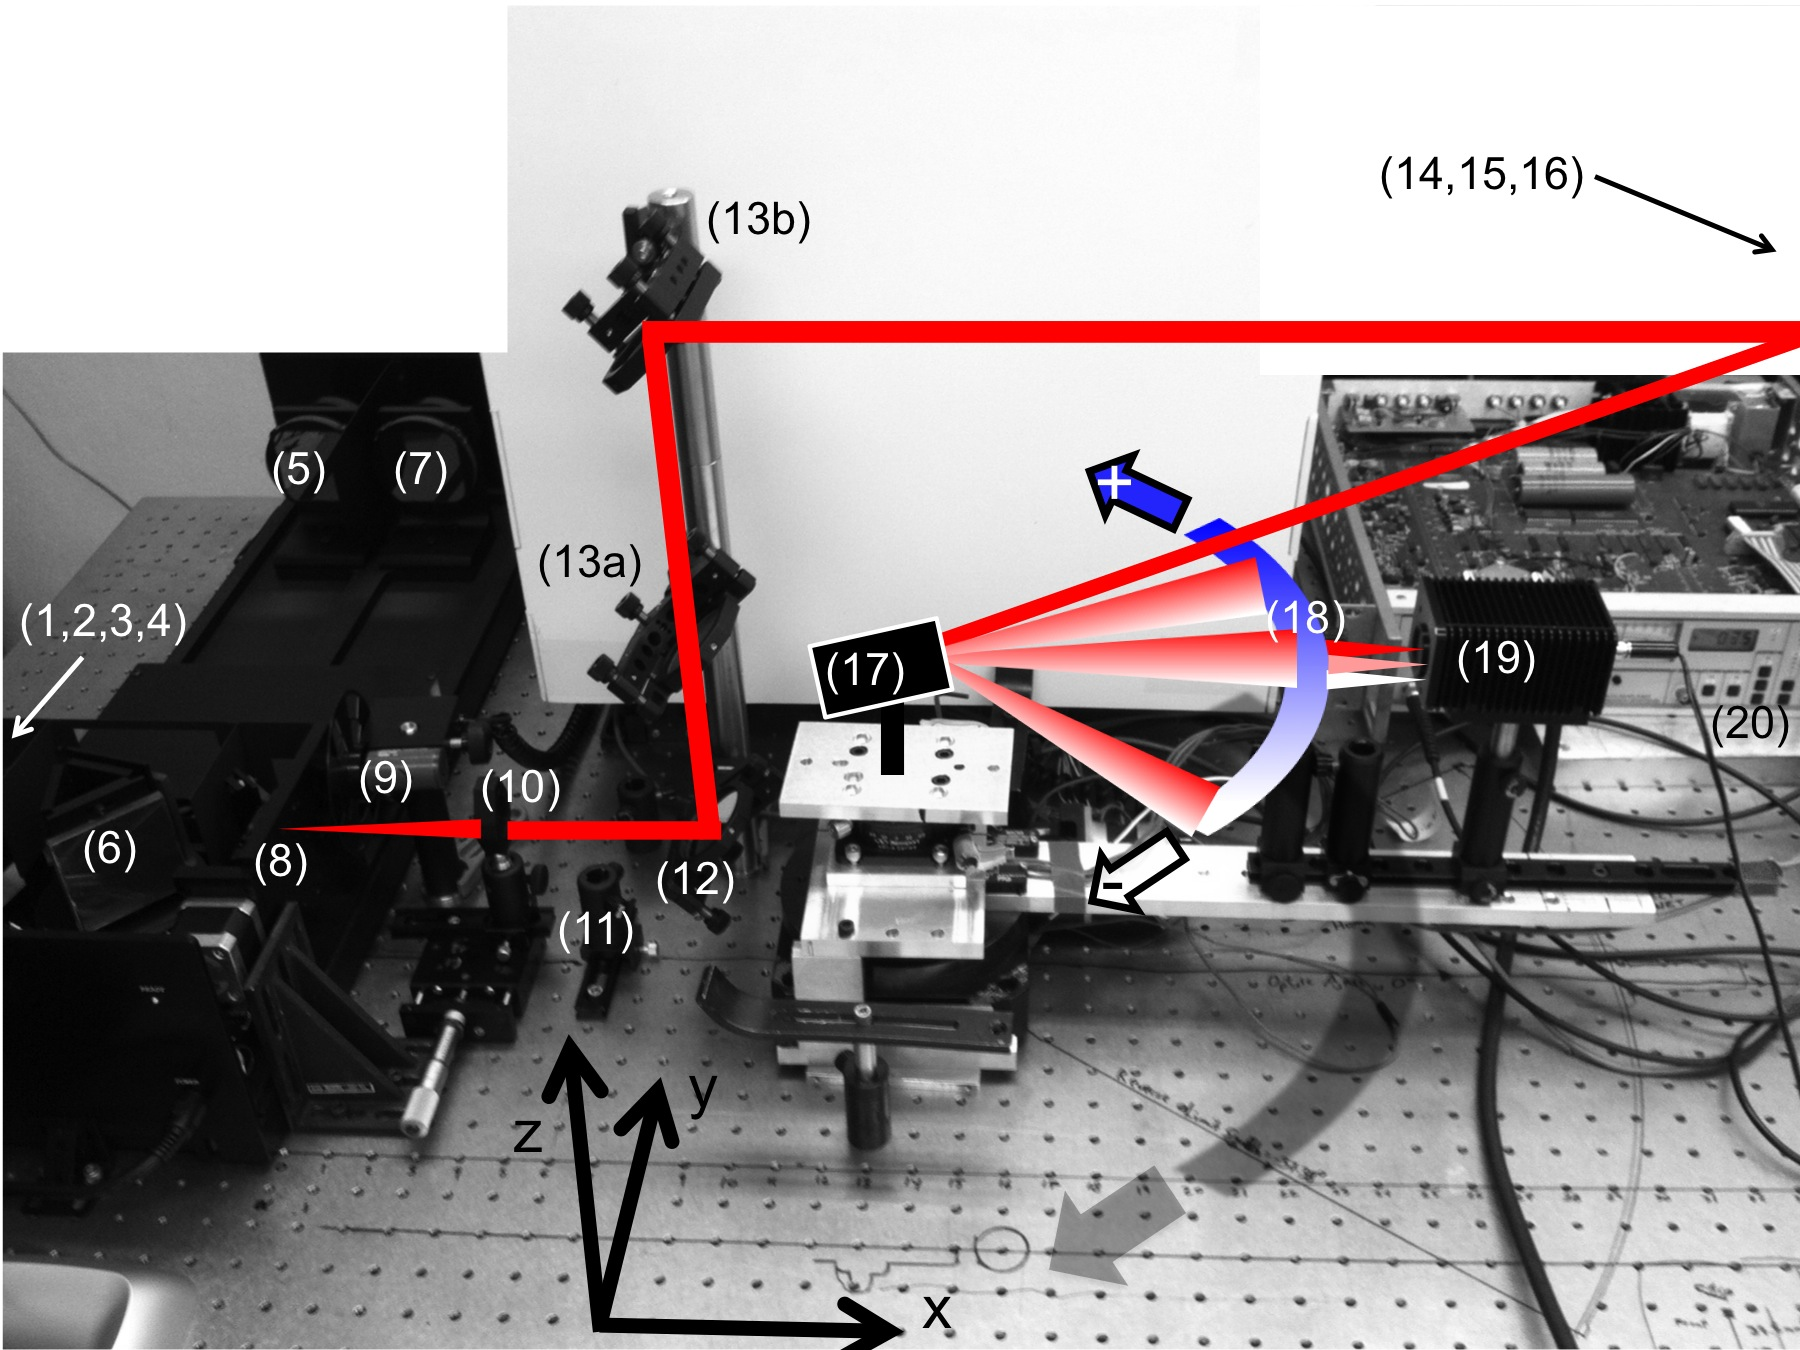
\includegraphics[width=1.0\textwidth]{chSPIE_2012_CA1/figs/GTA_cam_model_ref_tilt.jpg}
  \end{center}
  \caption[Schematic of the CROWBAR: Custom Robotic Order, Wavelength, and Blaze Angle Recorder]{\label{fig:GTAview} View of the monochromator, periscope, and swing arm-camera system with the beam path highlighted.  The beam exits the monochromator exit slit (8), where the optical chopper (9) is located.  The beam is collimated by a 1 inch post-slit lens (10).  The periscope system includes 3 mirrors (12, 13a, 13b), only two of which are active at any time.  In the reflective arm of interest to this report, we use mirrors (12) and (13b), with mirror 13a moved clear out of the beam path with a 90$^\circ$ flip mount.  The beam travels about 1 meter (off the image) to an adjustable iris in double pass (14, 16) sandwiching a mirror (15) tilted about 10$^\circ$ from the $z-y$ plane.  The beam travels along the vector terminating on the center of the immersion grating (17).  The immersion grating has its grooves vertical (parallel to the $z-$axis) so that the dispersion occurs in a the $x-y$ plane.  There are typically 3 or 4 orders diffracted $\pm20^\circ$ from the optical axis, for CA1 in our wavelength range of interest ($1.5-2.5 \; \mu$m).  The camera lens (18) and single pixel detector (19) are mounted on a swinging arm which rotates in the $x-y$ plane, with its center of rotation equal to the position of the immersion grating.  The angular range of motion of the swing arm is about +27 to -37$^\circ$ which is set by limit switches and the rigid mechanical structure, which supports the immersion grating and its concomitant fine adjust positioning hardware.  The cartoon arrows demonstrate our angular sign convention which is positive counter clockwise, with zero along the optic axis.  The grating normal is at about -70$^\circ$ with that convention.  The beam path in the monochromator is omitted for clarity.  The lock-in amplifier electronics are marked with number (20).}
\end{figure}


\chapter{High Performance Si Immersion Gratings Patterned with Electron Beam Lithography} 
\label{chap_ebeam}

\section{INTRODUCTION}
\label{sec:intro}  % \label{} allows reference to this section

At the 2012 SPIE Astronomical Telescopes and Instrumentation meeting (volume 8450) we described the detailed performance of the immersion grating (part number CA-1a \cite{2012SPIE.8450E..2SG}) for the high resolution infrared spectrograph IGRINS \cite{2010SPIE.7735E..54Y}.  IGRINS saw first light at McDonald Observatory in March 2014.  Papers describing its performance appear in the current volume\cite{2014SPIE.CHANPARK.IGRINS,2014SPIE.9151E..1GB}.  The technical readiness of the immersion grating now rests on firm footing, and our group has now moved on to pushing the performance and design limitations of silicon diffractive optics.  The key limitation is phase coherence.  Phase coherence for a diffraction grating is the accuracy to which repeated grating facets are positioned to an integer multiple of $\sigma$, the groove constant (the desired constant spacing from groove to groove).  Specifically, the position, $x$ of the $n^{th}$ facet in a sequence of $N$ total facets is distributed as: 

\begin{eqnarray}
x_n = n\sigma + \epsilon_n  \label{eqn:Epsilon}
\end{eqnarray}

where $\epsilon_n$ is the position error for facet $n$.  Discussion of the phase performance can be broadly separated by the correlations  of errors, $\epsilon_n$, and their impact on the monochromatic spectral purity.  


There are large scale, smooth correlations:
\begin{eqnarray}
\epsilon_n = \epsilon_n(x, y) \label{eqn:smooth}
\end{eqnarray}
These errors manifest as low order optical aberrations and degrade the PSF and Strehl.  Operationally these smooth errors correspond to the first $M$ Zernike polynomials in an orthonormal expansion of the wavefront, where $M < 200$.  There is the especially pernicious repetitive error:
\begin{eqnarray}
\epsilon_n = A\sin{\frac{2\pi n\sigma}{P} - \phi} \label{eqn:Periodic}
\end{eqnarray}
where $n\sigma$ is the desired position of the $n^{th}$ groove, $A$ is the amplitude of the error (e.g. in nm), and $P$ is the period of the error (e.g. in mm).  These errors manifest as sidelobes of the PSF called Rowland ghosts.  Although we have listed a single harmonic periodic error, any periodic structure can be broken into its Fourier components, so each of these Fourier components will be affiliated with a sidelobe Rowland ghost.  Lastly there are small scale random errors:
\begin{eqnarray}
\epsilon_n \sim \mathcal{N}(0, c)
\end{eqnarray}
where $ \sim \mathcal{N}(0, c)$ denotes that the error is normally distributed with mean zero and standard deviation $c$.  This last type of error produces so-called spectral grass\cite{2007ApOpt..46.3400M}, which is scattered light filling the blaze.

\section{On-sky performance of Si immersion grating}

With the commissioning of IGRINS \cite{2010SPIE.7735E..54Y}, we have demonstrated that the immersion grating performance measured in the laboratory translates into performance in a real world instrument in the field.  IGRINS is a high resolution near-infrared astronomical spectrograph.  It employs an immersion grating as its primary dispersive element, and two cryogenic VPH gratings for cross-dispersion.  The instrument covers a wavelength range of 1.5$-$2.5 $\mu$m in two channels.  The design and early performance of IGRINS is described in this volume [talk 9147-48]\cite{2014SPIE.CHANPARK.IGRINS}.  The immersion grating for IGRINS is internal part number CA-1a.  Its lab-measured performance is summarized in Gully-Santiago et al. 2012\cite{2012SPIE.8450E..2SG}.

IGRINS has no measured performance limitation attributable to the immersion grating.  CA-1a is diffraction limited.  CA-1a has been thermally cycled $>10$ times at the time of writing, with no perceptible degradation in performance.  We expect no degradation from thermal cycling.  We have previously constrained the CA-1a blaze angle to $\delta = 71.5\pm 0.2^\circ$.  The overall instrument throughput is consistent with the expected throughput including the laboratory-measured diffraction efficiency of CA-1a.

One major open question is whether CA-1a meets its spectral ghost level specification.  Spectral ghosts are secondary images that arise from periodic facet positioning errors\cite{2007sdf..book.....J}. The ghosts in CA-1a where introduced from a cyclically varying position-dependent exposure dose in the UV photolithography patterning step.  The processing error causing the ghosts has since been eliminated.  As a result our most recent immersion grating prototypes show a dramatic reduction in high frequency spectral ghosts [this volume, talk number 9151-35]\cite{2014SPIE.9151E..1GB}.  The ghost level depends on the amplitude of the error (cf. Equation 14 of Marsh et al. 2007\cite{2007ApOpt..46.3400M}):
\begin{eqnarray}
	\frac{I_g}{I_0}=[ \frac{2\pi n}{\lambda}A \sin{\delta} ]^2	 \label{eqn:GLevel}
\end{eqnarray}
where $I_g/I_0$ is the ghost level relative to the main peak, $\lambda/n$ is the wavelength scaled in the refractive index, and $A$ is defined in Equation \ref{eqn:Periodic}.  We predicted an in-immersion ghost level of $I_g/I_0 \sim2\times10^{-3}$ at 1.5 $\mu$m based on visible laser metrology\cite{2012SPIE.8450E..2SG}.  At the time of writing the IGRINS commissioning team has constrained ghost levels at $\lambda=1.5 \; \mu$m to $I_g/I_0 < 1\times10^{-2}$.  The limitation of a direct ghost level measurement is the need to deconvolve the slit diffraction ringing from the spectral point spread function.

\section{Motivations for direct writing Si immersion gratings}
We have determined experimentally that the lithographic transfer step is the most important determinant of the optical quality of Si immersion gratings.  The prior steps: orienting, polishing, passivating and resist-coating the monolithic substrates is now routine and our process control for these steps is sufficient to limit their contribution to the error budget to the point where they have no effect on the quality of the final gratings\cite{2007ApOpt..46.3400M,2014SPIE.9151E..1GB}.  The subsequent steps: development of the resist, reactive ion etching of the passivation layer, and anisotropic etching of the V-grooves similarly contribute little to the overall errors.  We therefore concentrate our efforts on finding more effective and accurate ways to carry out the transfer or patterning step.  

The JPL Microdevices Laboratory has an advanced electron beam writer (a JEOL model 9300FS) and has made an extensive effort to understand the nuances of using this device for precision patterning of small features over large spatial scales.  For the large-area immersion grating exposures we use the JEOL 9300FS at 100 kV accelerating voltage with 60 nA current, a spot size $\sim 100-150$ nm and spot step spacing of 50 nm. Our typical groove frequency for echelle grating prototypes is 40 - 12.5 grooves/mm (25-80 $\mu$m groove spacing) but groove frequencies higher than 1000 grooves/mm are possible. Experimental pattern sizes are up to 100 mm $\times$ 40 mm, but could be as large as 200 mm diameter.

\subsection{Motivation \#1: Higher precision than contact lithography}
\label{sec:Precis}
Electron beam lithography is more precise than contact lithography.  One figure of merit for precision in e-beam lithography is the \emph{spot size}, the typical diameter of the Gaussian e-beam current distribution at the location of the e-beam sensitive resist on the substrate surface.  E-beam spot sizes on the JEOL 9300FS tool can be as low as 4 nm at low currents (less than 1 nA).  To expose the required immersion spectrometer grating areas in reasonable times, tens of nA of current are needed, and $\sim 100 - 150$ nm spot sizes are typical.  The final precision is a small fraction of the spot size, since many adjacent spots are convolved together.  In later sections we directly compare the performance of immersion gratings produced with e-beam and contact lithography to show evidence that we have achieved much higher precision in e-beam lithography.  

\subsection{Motivation \#2: Finer groove pitch capability}
Owing to its small achievable spot size, electron beam lithography can reach finer groove spacings than contact photolithography can.  Fine pitches are required for high dispersion in low order.  Our group is currently designing a fine pitch ($\sigma \; \sim$ 2 $\mu$m, line frequency $\sim 500$ lines/mm) pattern immersion grating for the NASA Earth Science Technology Office (ESTO) Advanced Component Technologies (ACT) program.  The ACT mission concept requires high spectral resolution at low order ($\sim1-10$).  The desired first and second order gratings cannot be made with contact lithography.  Higher order devices can be made with contact lithography, but suffer from order overlap and reduced bandwidth.


\section{e-beam patterning strategies}
E-beam patterning takes place within a hierarchy of increasing scale-sizes.  The relationships of these pattern scale sizes affect the relative power distributed among spectral and spatial scales in the delivered monochromatic PSF.

\subsection{e-beam patterning scale size hierarchy}

\begin{figure}
\begin{center}
 \begin{tabular}{c}
    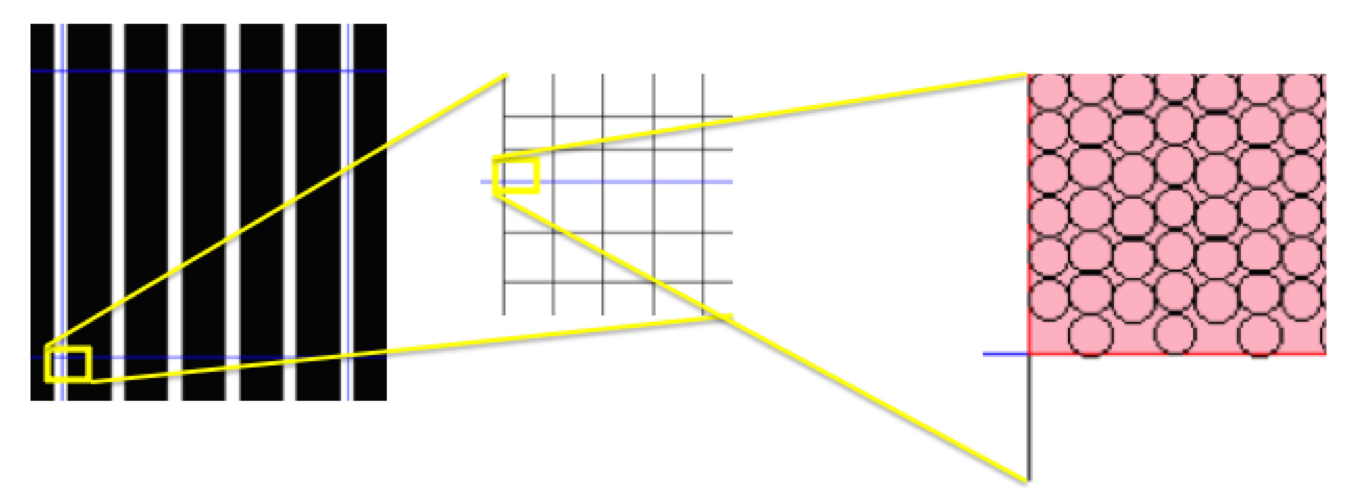
\includegraphics[width=0.8\textwidth]{chSPIE_2014_ebeam/figs/Field_sizes_cascade_02.png}
   \end{tabular}
  \end{center}
  \caption[e-beam Hierarchy]{\label{fig:Hierarchy} Hierarchy of e-beam pattern scale sizes- in the left panel the grooves are black and the fields are thin blue lines, the middle inset shows subfields, and the right inset shows spots at a regular step spacing, though the spots are not to scale.  Spot sizes are typically about 2-3 times their spacing.}
\end{figure}


There are a five key pattern scale sizes in e-beam lithography.  These scales are typical among e-beam tools, though we focus our discussion to the scales relevant to the JEOL 9300FS.  The scale sizes in order of small to large scales are 1) step size, 2) spot size, 3) subfield deflector size, 4) field deflector size, and 5) stage range of motion.  Figure \ref{fig:Hierarchy} shows a cartoon of the hierarchy from left to right- field, subfields, and steps.

Table \ref{tab:D07andE12} lists the pattern size scales for two immersion grating prototypes, parts D07 and E12.  These prototypes are examples of successful pattern designs.  D07 and E12 were both patterned on 10 mm thick Si pucks.  A 10 mm thickness is sufficient for the piece to maintain its flatness after anisotropic etching of the grooves so that interferometric measurements will reflect accurately the effectiveness of the patterning step.

\begin{table}
	\begin{center}
	\caption{D07 and E12 e-beam pattern details. \label{tab:D07andE12}}
	\begin{tabular}{ccc}
	\toprule
	   &D07 & E12  \\
	\midrule
	substrate bias angle ($^\circ$) & 6.1 & 71.5 \\
	pattern size (mm) & 39.0 x 39.664 & 29.696 x 84.816 \\
	pitch ($\mu$m) & 7.8 & 27.36 \\
	line frequency (lines/mm) & 128.2 & 36.55 \\
	top width ($\mu$m) & 0.4 & 9.96 \\
	line width ($\mu$m) & 7.4 & 17.40 \\
	step size (nm) & 50 & 50 \\
	steps per linewidth & 148 & 348 \\
	subfield size ($\mu$m) & 3.7 & 2.9 \\
	subfields per linewidth & 2 & 6 \\
	steps per subfield & 74 & 58 \\
	\cline{1-1}
	 			      & 63: 491.4  & 17: 465.12 \\
	grooves per $x-$field and & 61: 475.8 & 15: 410.4 \\
	$x-$field sizes ($\mu$m) & 59: 460.2 & 13: 355.68 \\
	 				        & 55: 429.0 & 11: 300.96 \\
	\cline{1-1}					        
	 			      & 134: 495.8  &   \\
	subfields per $y-$field and & 133: 492.1 &   \\
	$y-$field sizes ($\mu$m) & 131: 484.7 & 160: 464.0 \\
	 				        & 127: 469.9 &   \\	
	\cline{1-1}
	\bottomrule
	\end{tabular}
	\end{center}
\end{table}	


\subsubsection{e-beam step size and spot size}
The e-beam step size is the center-to-center separation of the e-beam spots, controlled by the beam-deflection electronics of the writer.  Step sizes can range from roughly 2 to 100 nanometers.  We adopted a 50 nm step size for our immersion grating patterns.  The rationale for the step size depends on understanding the e-beam spot size.  

The spot size controls the smallest achievable feature size.  Our spot size of $\sim 100 - 150$ nm is determined by operational properties of the electron gun and focusing column.  The spot size can be decreased by preferentially removing those electrons with large velocity components perpendicular to the bulk direction of motion.  This preferential removal of fast electrons is achieved with a grounded conductive circular aperture in the beam path prior to the spot formation.  The aperture is constricted to reduce the spot size.  The net current (e$^-$/s) consequently decreases, since the aperture has effectively thrown away electrons.  So there is a tradeoff between current and spot size.  This tradeoff is important in deciding optimal patterning strategies and sizes.  The economical need to limit the expensive e-beam write time necessitated a high current and hence the resulting large spot size.

The conductive aperture setting coarsely selects the range of spot size achievable, while the detailed spot size depends on fine adjustments made to the e-beam column before an exposure.  These adjustments are familiar for those who have used scanning electron microscopy- astigmatism, wobble, and focus, for example.  Poor calibration might deliver an elliptical, asymmetric spot shape.  In practice, a slightly asymmetric spot shape does not affect the performance of immersion gratings.

A key idea is that the step size (50 nm) is much smaller than the spot size so that adjacent steps convolve to form a fairly uniform exposure area.  Another key assumption is that the e-beam spot does not change significantly over the course of an exposure.  We expect that the e-beam spot is unchanged, so long as the e-beam column is unperturbed.

\subsubsection{Subfield deflector}
The subfield deflector is a component of the e-beam gun that directs the e-beam spot within a box of up to 4 $\mu$m $\times$ 4 $\mu$m, centered around a mean position set by the main field deflector.  For example we chose subfield sizes of 3.7 and 2.9 $\mu$m for D07 and E12, respectively.  For recent work on fine pitch ($\sim2\; \mu$m) gratings we have experimented with smaller subfield sizes.  The reason for these choices of subfield sizes of D07 and E12 is that these field sizes result in an integer number of subfield per linewidth, which avoids fractional e-beam spots at the boundaries.  Subfield boundaries are perceptible in the intentionally underexposed e-beam resist of sample TJ04, depicted in Figure \ref{fig:TJ04Zeiss}.  In general we have found subfield stitching boundaries do not cause measurable ghosts unless the choice of subfield size results in fractional spots at the subfield/field boundaries.  

\subsubsection{Field deflector}
\label{sec:Field}
The field deflector, also sometimes called the main-field deflector, coarsely redirects the electron beam over a square up to 500 $\mu$m in size.  The main-field deflector positions the center of the subfields.  For example, the choice of a 500 $\mu$m square field size and 4 $\mu$m square subfield size would result in 125 $\times$ 125 subfields.

The fields are stitched together by the interferometrically controlled stage that steps between them once each field's pattern has been written.  The stage move speed is typically much slower than the field and subfield deflector speed, so small field sizes are inefficient in time-on-target compared to wall-clock time.  Even though the JEOL 9300FS dynamically corrects for beam position distortion (e.g. pincushion) and spot focus and astigmatism, the writing performance degrades slightly with distance from the center of the field.  So there is a tradeoff between write speed and performance.  

The choice of field size is multifaceted.  Field size choice is one of the key strategies for mitigation of ghosts (see Section \ref{sec:Ghosts}).

\begin{figure}
\begin{center}
 \begin{tabular}{c}
    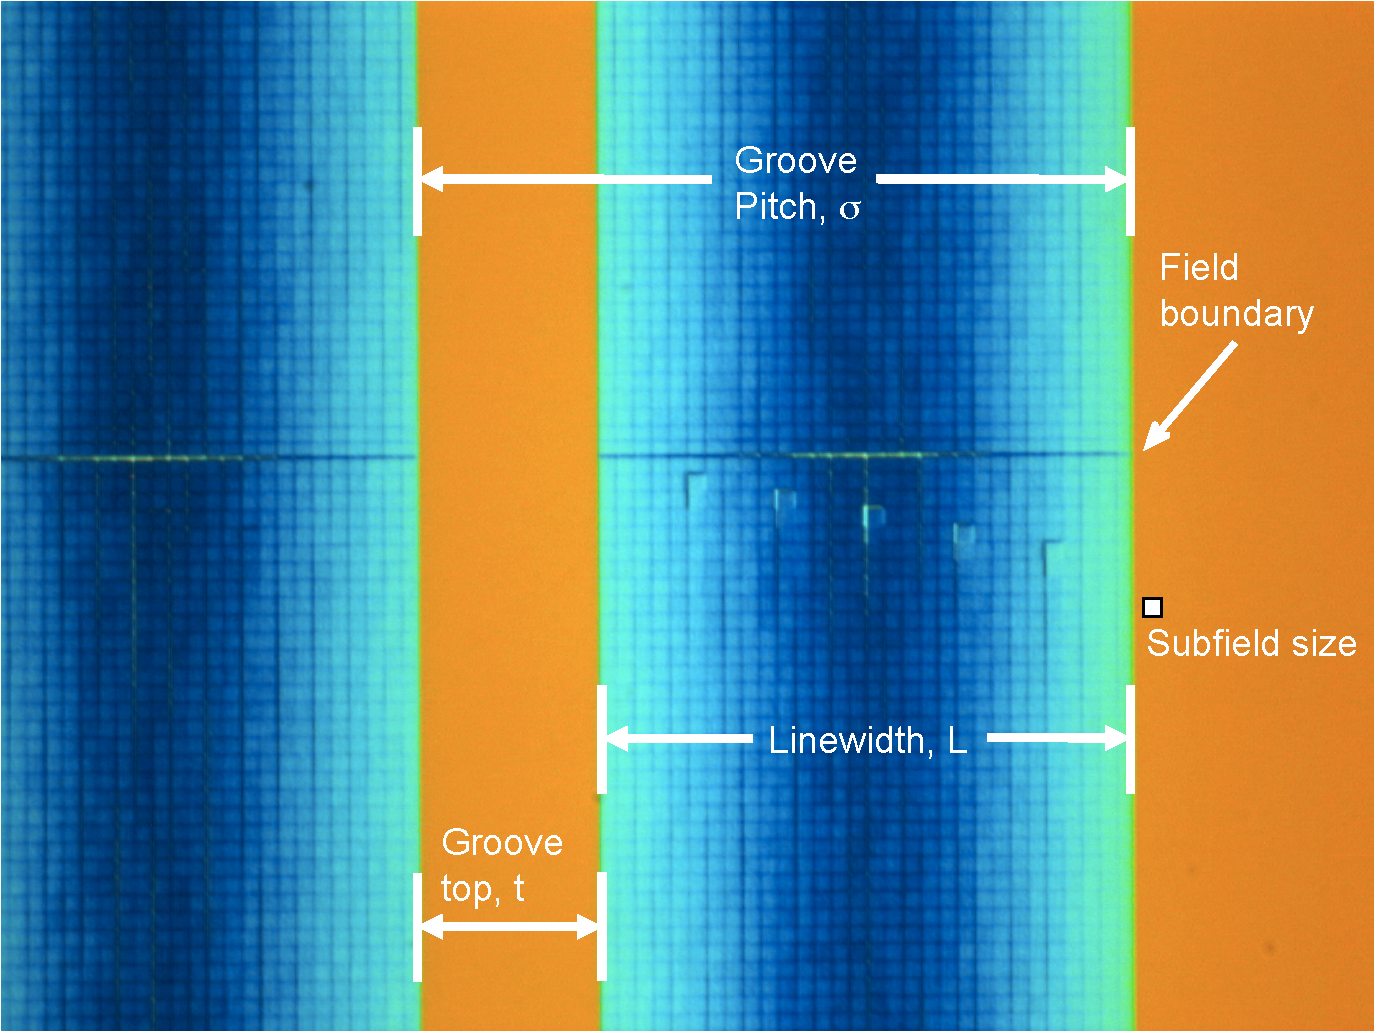
\includegraphics[width=0.96\textwidth]{chSPIE_2014_ebeam/figs/subfields_TJ04_Zeiss.pdf}
   \end{tabular}
  \end{center}
  \caption[TJ04 under Zeiss]{\label{fig:TJ04Zeiss} Subfield and field boundaries directly perceptible in optical microscopy of the e-beam resist on an intentionally underexposed sample, TJ04.  The groove pitch for this sample is 100 $\mu$m, with a 75 $\mu$m written linewidth.  The blue area is the linewidth portion of the grating which has e-beam resist already exposed to e-beam.  The orange line is the groove top, where the e-beam resist was unexposed and would have served as the wet etch dam, had the linewidth actually developed out.  The minute color differences within the exposed linewidth are attributable to tiny thickness differences of the resist, which originate from tiny differences in delivered e-beam dose.  The cylindrically symmetric color difference of teal to dark blue is attributable to the proximity effect as described elsewhere\cite{2005SPIE.5720...68W}.  The tiny boxes are subfields, which are only perceptible due to subtle subfield stitching errors.  Some subfields are more errant than others.  The thick horizontal stripe is a portion of a much larger field boundary, perceptible only because of main-field deflector stitching boundaries as discussed in the text.}
\end{figure}

\subsubsection{Interplay of hierarchy at boundaries and design rules}
\label{sec:Boundaries}
Undesirable repetitive patterns that can cause ghosts arise when there are discontinuities as one steps up the field hierarchy.  The e-beam spots, subfields, and fields must match up at the boundaries.  We learned many subtle design rules unique to high performance immersion gratings.  The main theme in all of the design rules is to avoid fractional steps in the writing process.  The JEOL pattern generation software inserts patterns of spaces and spots when it reaches a command for a fractional step.  The specific design rules below are probably unique to the JEOL pattern generation software.  Other e-beam tool software is likely to have different design rules, but the general principle is the same.  
\begin{enumerate}
  \item Subfields must be an integer number of steps
  \item Fields should be an integer number of subfields.  
  \item Linewidth should be an integer number of subfields.
  \item Field sizes and linewidths can be non-integer number of subfields only if the remainder fractional subfield plus one subfield divided by two is an integer number of step sizes.
\end{enumerate}   

These rules ensure that all e-beam spots are equidistant.  Figure \ref{fig:Hierarchy}  shows the JEOL \emph{shot shape display} of a pattern that broke rules 2 and 4.  Metrology of a grating prototype that broke rules 2 and 4 resulted in cross-dispersion grating ghosts $>10^{-3}$.  The line-edge of contiguous spots lacked a solitary spot near the subfield boundary.  Such a periodic dearth in exposure manifested as a periodic divot along the length of the groove.  The detailed impact on optical phase depends on the relative step size, e-beam sensitive resist contrast, and sundry subsequent processing steps.  Rather than risk a performance degradation it is best practice to avoid the formation of subfield blips in the first place.  The main concern for a final application is probably scattered light, and not efficiency loss. 


\subsection{Predicting the ghost level associated with field positioning errors}
\label{sec:Ghosts}

The field size is only a few times larger than our typical coarse echelle grating groove constants.  Figure \ref{fig:FieldCartoon} shows an exaggerated cartoon of the field size relative to grooves.  In a hypothetically perfect e-beam field stitch, the line positions are exactly as desired.  In reality there is some finite distortion, which is repeated each time the field is written into the e-beam resist.  We define the ratio, $G$, as the field size, $F$, divided by the groove pitch size, $\sigma$.  For example, there will be $G=500/100=5$ grooves per field for $\sigma = 100 \; \mu$m and $F = 500 \; \mu$m.  The omnipresent field deformations will be imprinted into each field, repeating every 5 grooves.  The cyclically varying facet positions manifest as ghosts with G-fold symmetry. We expect $G-1$ inter-order ghosts, separated by a fraction $1/G$ of the inter-order separation.


\begin{figure}
\begin{center}
 \begin{tabular}{c}
    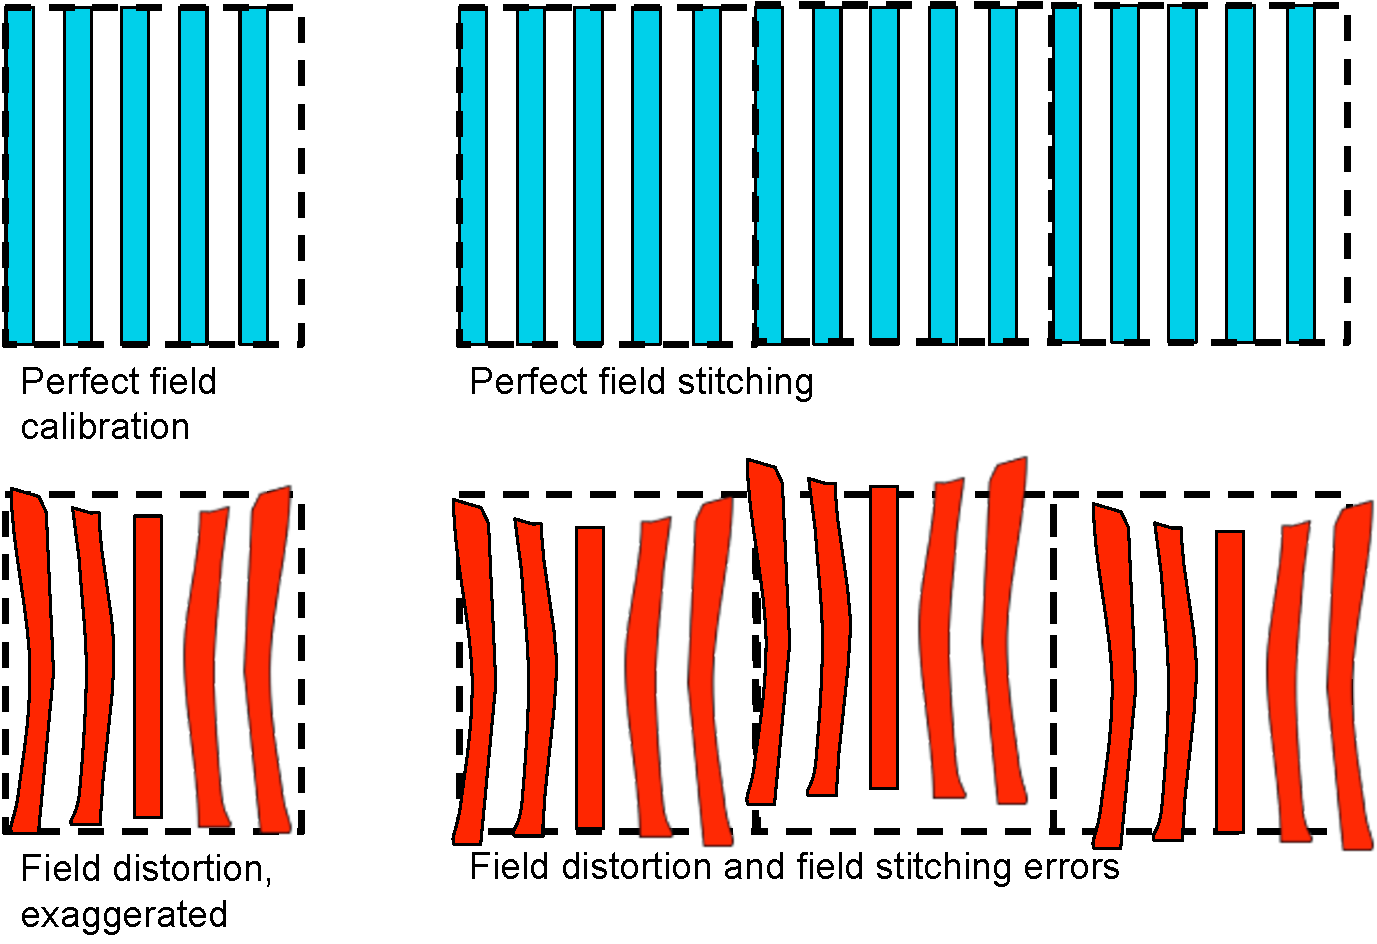
\includegraphics[width=0.6\textwidth]{chSPIE_2014_ebeam/figs/Field_stitching_errors_alt2.pdf}
   \end{tabular}
  \end{center}
  \caption[Field Stitching Error Cartoon]{\label{fig:FieldCartoon} An exaggerated cartoon to demonstrate the repetitive nature of field stitching.  A typical field size is about 300-500 $\mu$m on a side, and typical groove periods, $\sigma$, are about 20-100 $\mu$m (50-10 lines/mm groove frequencies).  Here we show 5 grooves per field.  The distortion shown in the cartoon is highly exaggerated, and in reality the calibration is much, much better than depicted.  The center positions in the distorted fields are distributed around the target, demonstrating field stitching errors.  The actual morphology of the distortion is not well characterized and should be mostly corrected by the 9300FS dynamic distortion correction system.  We have depicted a pincushion shape, though the realized morphology could be more like barrel distortion or a parallelogram.  The fields could also be perfectly square and simply misplaced in their center positions, still causing errors.  The details of the morphology give rise to differing relative levels of harmonics, in a Fourier sense.  To put the scale in perspective, we coarsely estimate the repetitive position error amplitude A (cf. eq. \ref{eqn:Periodic}) as about 5-50 nm from experiments on e-beam wafers.  Compare this minuscule position error with the $\sim500 \; \mu$m field size, to see that the fractional position error is 1 part in $10^4$ or better.}
\end{figure}

In principle it is possible to predict the ghost levels relative to the main diffraction peak, given some information about the magnitude and shape of the field distortion.  As the amplitude of the field distortion is dialed up, the grating ghost level increases approximately as Equation \ref{eqn:GLevel}.  In practice, we have not directly mapped the field distortion, which we expect to be a function of both $x $ and $y$.

\subsection{Employ multiple field sizes rather than one field size}
\label{sec:MultipleFields}
There are two strategies for mitigating ghosts.  One is to reduce the overall power in ghosts, using a single field size.  The other is to redistribute the power into different spatial scales, by using a variety of field sizes.  The strategies can be combined.

We redistribute the field power into several different spatial scales following the method described in Wilson et al. 2005\cite{2005SPIE.5720...68W}.  Rather than use a single field size, say 500 $\mu$m, we break up the field into several fields, say 500, 450, 400, and 350 $\mu$m.  We array the fields on the pattern in the following way.  We divide up the overall grating pattern, for example 30 mm $\times$ 85 mm, into eight long thin stripes of 3.75 mm $\times$ 85 mm.  We then array the long thin stripes on top of each other, cycling through the patterns twice.  So if we have patterns A, B, C, D, with unique field sizes, we cycle through from top to bottom: A, B, C, D, A, B, C, D.  The reason for this periodic boundary condition is to make sure that the circular beam samples the patterns in roughly equal proportions.  Specifically, if we had simply written four arrays of dimension 7.5 mm $\times$ 30 mm, indexed as A, B, C, D, then the circular beam would underfill patterns A and D at the bottom and top.  The optimal strategy would probably be to randomly array fields, but in practice randomly arraying is non-trivial in existing software.

One way to reduce the overall power in a single field size is to select a small field size, say $F=$ 200 $\mu$m.   We know that the e-beam field performance is better in the center, and deviates towards the edge of the field.  The tradeoff with this strategy is that the stage move time is long compared to the e-beam field deflector time, so the write duration increases.  Another strategy for reducing the power in ghosts attributable to a single field size is to improve the intra-field calibration.   We could remove, for example, the minute pincushion or barrel distortion familiar from cathode ray tube computer monitors.  In practice it is tricky to measure, and therefore correct for, these minuscule distortions.  The absolute best way to eliminate inter-order ghosts is to use a field size equal to the pitch.  The choice of $F= \sigma$ is generally cost prohibitive for $\sigma <100$.  If long, inefficient write times can be tolerated, then in principle there is no limit to this strategy.  It is conceivable that driving the stage so much would make the stage fail over time.

Another strategy for reducing the overall power in spatial distortions of e-beam fields is to experimentally determine the optimal height offset for the e-beam focus.  For an unknown reason, the JEOL 9300FS selects a default writing height which is offset from the optimal height.  We experimentally verified an offset which reduces the overall distortion in the fields.

Lastly, there are some slightly obscure JEOL e-beam commands relevant to ghost mitigation.  These are the ``overlay'', ``gather'', and other affiliated commands.  The main idea behind these writing strategies is to re-write over a patch of grating so that it sees different portions of the field, and therefore the field distortions average down.  We experimented with these techniques but found that they roughly double the write times with negligible performance benefit.  


\subsection{Strategies for mitigating facet position errors attributable to large scale stage drift}

The largest scale in the e-beam writing hierarchy is the stage motion.  Multiple tests have never revealed significant wander or runout error in the interferometrically controlled stage.  Secular drift of the e-beam stage, however, can cause large-scale facet position errors which manifest as optical aberrations.

\subsection{Characterization of e-beam stage drift}
We characterized the e-beam stage drift with built-in JEOL commands.  Specifically, we used the \emph{DRIFT} and \emph{CURRENT} commands.  The \emph{DRIFT} command checks the position of the stage by scanning a precision gold cross mark mounted to the stage.  The process ties the actual position to the predicted position to the precision of the stage mark's centroid, which is a small fraction of the spot size.  We measured a precision of about 15 nm in the centroid process.  Having determined the amplitude and direction of the drift, the \emph{DRIFT} command subtracts out the offset and continues writing with its updated coordinates.

The centroiding \emph{DRIFT} process can be automatically repeated on a desired frequency.  We set a frequency of 10 minutes.  For a typical 20 hour write we achieve 120 drift corrections.  The JEOL software logs these corrections, so we can reconstruct the path of the drift, had we not taken action to correct it.  Figure \ref{fig:ebeamDrift} shows one of these reconstructions for sample E12.  The amplitude of the drift is  $\Delta x = $ 206 nm and $\Delta y = $ 341 nm.  This amplitude is much larger than we can tolerate for diffraction limited performance in immersion the near-IR.  

\begin{figure}
\begin{center}
 \begin{tabular}{c}
    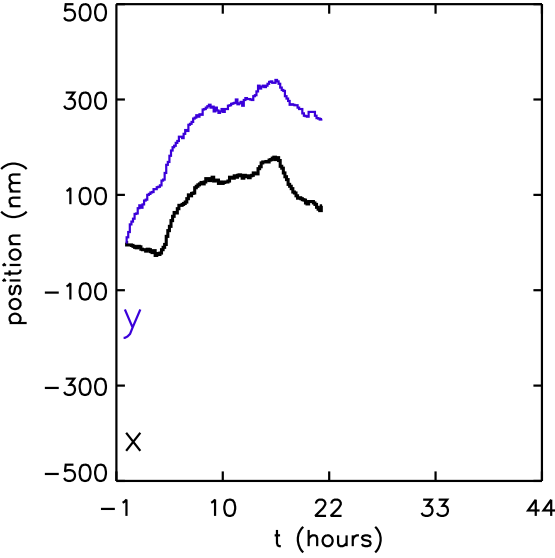
\includegraphics[width=0.4\textwidth]{chSPIE_2014_ebeam/figs/E12_drift_ebeam.png}
   \end{tabular}
  \end{center}
  \caption[Drift amplitude]{\label{fig:ebeamDrift} The reconstructed drift of the JEOL 9300FS e-beam stage during the patterning of sample E12.  The write time was 20.9 hours, with drift samples every 10 minutes.  The $x$ and $y$ components are separated and plotted as a function of time.  The top curve is the $y$ drift.  The curves begin at 0 at time zero, and show a range of motion of $\Delta x = $ 206 nm and $\Delta y = $ 341 nm.  This amplitude of drift would have been catastrophic for a grating which has line edge specifications of $\lambda/10 \sim 60 $ nm for diffraction limited performance in $J-$ band.  The JEOL9300FS command \emph{DRIFT} automatically corrects out this drift, so the maximum realized drift is merely the minuscule difference that occurs over the 10 minute interval between corrections.  Figures \ref{fig:E12igram} and \ref{fig:E09igram} show a direct comparison of prototype gratings patterned with and without drift correction.}
\end{figure}

A possible explanation for the beam drift is that there is thermal expansion attributable to heat conduction from the warm Si puck and holder unit into the stage.  Specifically, there is some evidence that the drift rate is largest at the beginning of the writing, perhaps while thermal equilibration is still happening.  The thermal probes on the stage lend some credibility to this idea, since the probes asymptote to constant value after a few hours.  Owing to this possibility, we recommend delaying the start of a write until the sample and holder have come into thermal equilibrium with the stage.  Beyond this thermal explanation, there are many conceivable reasons why there could be drift.  At some level we do not care, as long as we can correct it out sufficiently well.  The cost of correction is merely a hit in extended write time for the same written area, i.e. a decrease in efficiency.  We found roughly a 10\% overhead associated with drift checking.

\section{Results: Test gratings produced with e-beam patterning}

\subsection{Measurement of ghost levels for a variety of writing strategies}
\label{sec:MeasGhost}
In Figure \ref{fig:GhostLevelFig} we show measurements of inter order ghosts for different trial runs of the writing process with internal designations TJ03 and TJ04.  Each grating received a different treatment for e-beam field and/or subfield sizes.  The grating pattern details are listed in Table \ref{tab:TJ04details}.  The first thing to notice is that virtually all ghosts are below 10$^{-3}$ of the main peak.  Some ghosts were expected but not detected (denoted ND in the plot legend).  The non-detections are probably related to instrumental limitations, though upper limits are not available.  

\begin{landscape}

\begin{table}
	\caption{Wafer TJ04 pattern details.  \label{tab:TJ04details}}
	\begin{tabular}{lllcccccccccc}
	\toprule
	 &   & & \multicolumn{10}{c}{Grating Area} \\
	\cmidrule(l){4-13}
	Size Scale & & Unit & A  & B & C & D & E & F & G &  H &  I & J\\
	\midrule
	\multirow{2}{*}{Pattern length}& (x) & mm &  \multicolumn{10}{c}{15} \\
	 & (y) & mm & \multicolumn{10}{c}{10} \\
	Pitch && $\mu m$ & \multicolumn{6}{c |}{100} &\multicolumn{4}{c}{25}  \\
	Linewidth && $\mu m$ & \multicolumn{6}{c |}{75} & \multicolumn{4}{c}{22.5}  \\
	\multirow{2}{*}{Field}&(x) & $\mu m$ & 100 &  200 & 200 & 200 & 500 & Multi & 100 & 200 & 500 & Multi \\
	&(y)& $\mu m$ & 500 & 500 & 100 & 250 &  500 & 500 & 500 & 500 &500 & 500\\
	Subfield && $\mu m$ & 2.5 & 2.5 & 4.0 & 4.0 & 2.5 & 2.5 & 2.5 & 2.5 & 2.5 & 2.5 \\
	Spot && nm & \multicolumn{10}{c}{$\sim300$} \\
	Step && nm & \multicolumn{10}{c}{50} \\
	\bottomrule
	\end{tabular}
\end{table}

\end{landscape}

\begin{figure}
\begin{center}
 \begin{tabular}{c}
    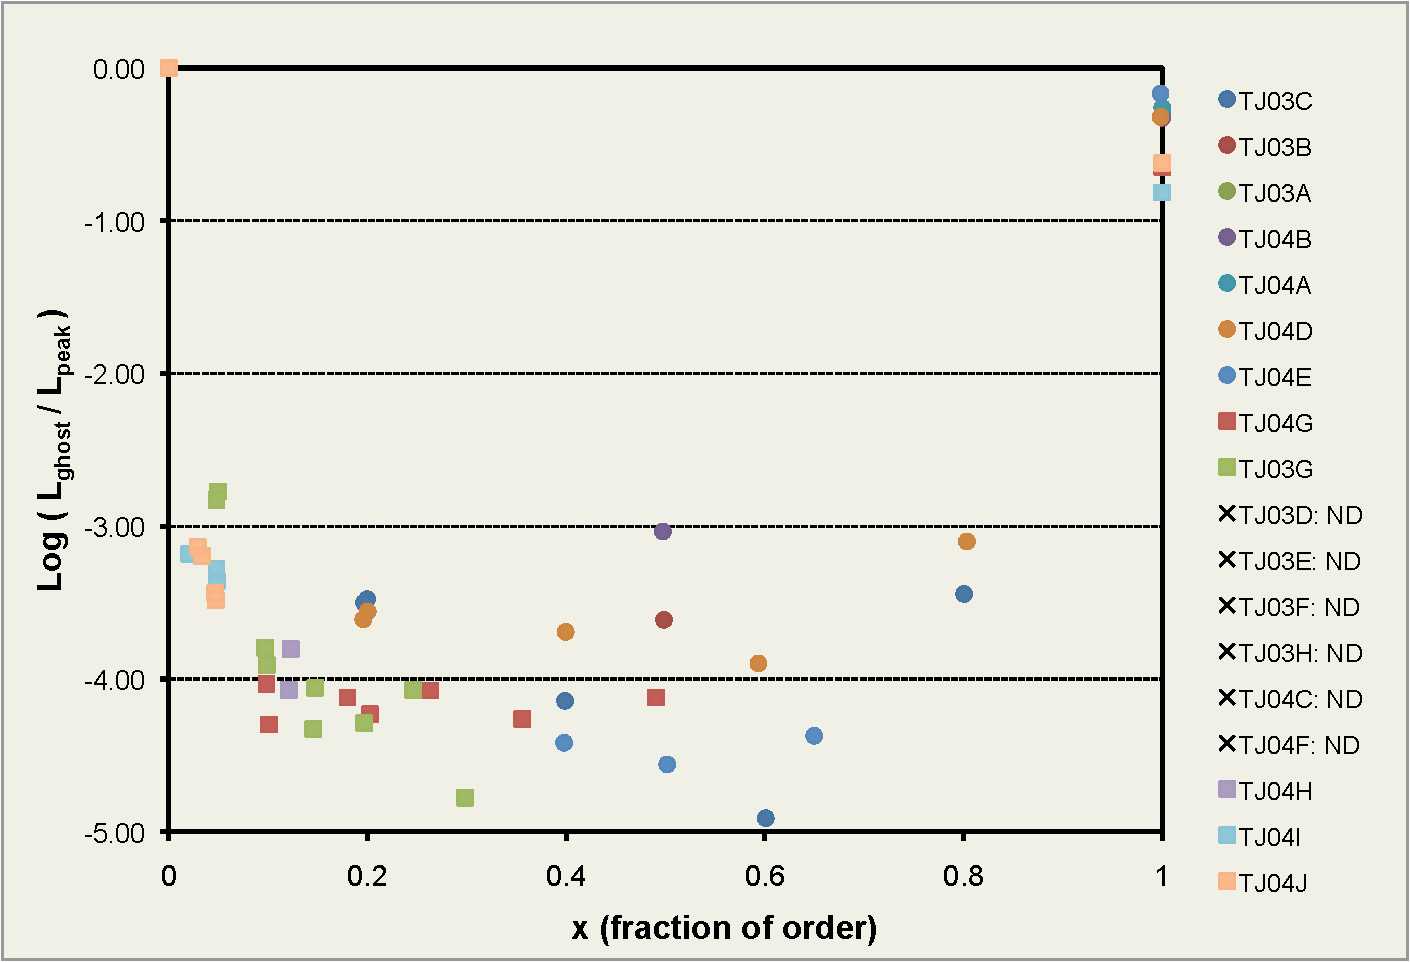
\includegraphics[width=0.8\textwidth]{chSPIE_2014_ebeam/figs/TJ04_ghosts_pretty_alt.pdf}
   \end{tabular}
  \end{center}
  \caption[Ghost level measurements]{\label{fig:GhostLevelFig} Measurements of the levels of inter-order ghosts for different trial runs of the writing process with internal designations TJ03 and TJ04.  The levels are normalized to the brightest order.  A full order is shown, with the $x-$axis units normalized to an order spacing.  The grating sub-areas of TJ04 are described in Table \ref{tab:TJ04details}.  Some ghosts are not detected, noted as ND.  The non-detections are due to instrumental limitations or genuine absence of ghosts.  The key idea here is that field size choice determines the number of- and to some extent the intensity of- inter order ghosts.  The absolute best patterning strategy is to set your $x-$field size equal to your groove pitch $\sigma$, as in TJ04A, which has no inter order ghosts.  All other patterns have a finite, albeit low, intensity ghost.  }
\end{figure}


\subsection{Improvement in wavefront performance from drift correction}
In Figures \ref{fig:E09igram} and \ref{fig:E12igram} we show the dramatic impact of drift correction on the performance of our Si gratings.  The stark difference in final wavefront error of the complete grating with drift correction and without drift correction is the ``smoking gun'' that the e-beam must have drift correction enabled to achieve high performance diffraction limited performance.  At the time of writing we have produced and tested another grating, G07, with even higher performance than E12.  Specifically, we perform interferometry at 632 nm in reflection with a 25 mm circular beam on a grating with a blaze angle of 71.6$^\circ$.  The measured wavefront error is $<0.10$ waves peak to valley for G07.

\begin{figure}
   \subfloat[E12 Interferogram]{\label{fig:E12igram}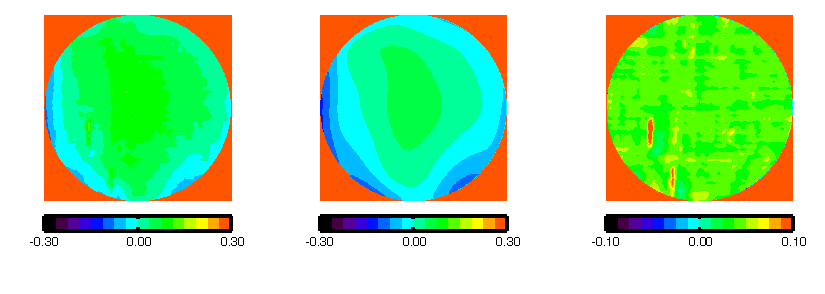
\includegraphics[height=5cm]{chSPIE_2014_ebeam/figs/E12_fig_scl2.pdf}}
   \newline
  \subfloat[E09 Interferogram]{\label{fig:E09igram}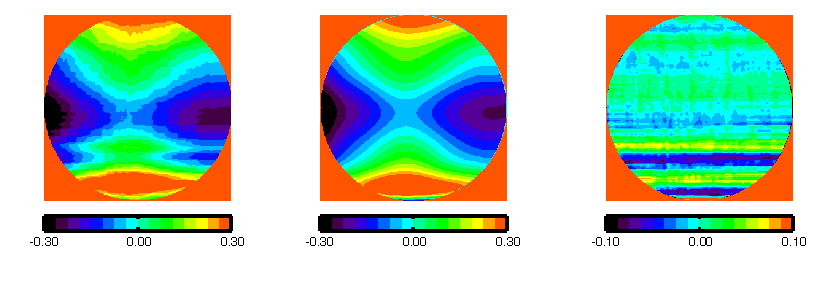
\includegraphics[height=5cm]{chSPIE_2014_ebeam/figs/E09_fig_scl2.pdf}}
  \caption[Interferometry reveals dramatic improvement in performance of e-beam produced immersion gratings]{Comparison of immersion grating surfaces on samples E09 and E12 measured with $\lambda = 632.8 $ nm interferometry.  These are both e-beam produced immersion grating surface prototypes.  The color scale is reported in fractions of waves of surface deviation.  The patterns on E09 and E12 are identical: $\sigma = $ 27.36 $\mu$m (about equal to 36.55 lines / mm), with a 9.96 $\mu$m groove top.  The groove top is not shadowed in these measurements which are taken in reflection in air, but we assume the groove tops have negligible impact on the measured interferometry.  The interferometry is performed with a 25 mm circular beam, which is projected over an 80 mm $\times$ 25 mm ellipse at the R3 echelle blaze angle, $\delta = 71.5 ^\circ$.  The left panel is the measured interferometry.  The middle panel is a decomposition into the first $\sim 80$ Zernike terms.  The right panel is the residual.  E09 was written on May 4, 2011, E12 was written September 1, 2011.  The only difference between the samples is that E12 was written with \emph{DRIFT} and \emph{CURRENT} check protocols with the JEOL e-beam writing software.  E09 was written without \emph{DRIFT} and \emph{CURRENT} check protocols.  The outcome is dramatic- E12 has $\sim 4$ times lower surface deformation than E09.  Note that the vertical color bars are on the same scale to ease visual comparison.}
  \label{fig:igrams}
\end{figure}


\section{Limitations of direct writing Si immersion gratings}
Electron beam lithography outperforms UV contact mask photolithography, at least in terms of the important metric of large scale phase coherence.  There are tradeoffs in pursuing e-beam lithography over UV contact mask photolithography.  We highlight some of these tradeoffs here.

\subsection{Serial write process yields long write times}
One key tradeoff is that e-beam lithography is a serial write process, whereas UV contact mask photolithography is a parallel write process.  A contact mask exposure takes about 1-2 minutes, whereas a e-beam exposure takes about 20 hours, for 30 mm $\times$ 80 mm patterns.  The problem is even worse if you scale to larger areas, for the next generation immersion gratings.  The high hourly expense of e-beam time makes the writing process the dominant expense over all other preparation steps, despite the high per-part cost of the large precision-oriented and optically polished monolithic Si pucks.  

\subsection{Large per-part investment cost yields heightened process risk}
In reality, the expensive e-beam writing process is not more expensive than procuring a custom high precision vendor-provided photomask.  E-beam lithography simply has a higher per-part risk than UV contact mask photolithography.  Processes after the e-beam step better be low-risk.  Specifically, the processes after exposure include: discharge layer removal, development, plasma etching, wet etching, and shaping.  We find that plasma etching responds differently to thick samples, probably due to the large difference in strike height and dielectric differences between vacuum and Si.  In one case, an overactive plasma etch burned away all the e-beam resist on a 30 mm thick Si sample.

\subsection{Experiments with negative resist}
There is an steep tradeoff in precision and write time.  There is not much way around this tradeoff except for one recent idea of replacing positive tone resist with negative tone resist.  Recently we have experimented with low order Si immersion gratings with groove pitches on the order of $2 \; \mu$m (groove frequency $\sim500$ lines/mm), and and groove tops on the order of 100 nm.   The small pitch and groove top require a small spot size, and therefore a small step size.  We decreased our step size from 50 nm to 10 nm.  This change alone drives up the write time by a factor of 25.  To counteract the otherwise impossibly high write time, we have experimented with negative tone resist.  Negative resist is cleared where the resist is unexposed, and remains only where the resist is exposed.  Since the fill factor of written to unwritten is a factor of 20, the negative resist makes possible the e-beam lithography of these fine pitch patterns.  

In principle these gains from negative resist could be extended to immersion echelles.  Specifically our typically modus operandi has been to clear about 65\% of the open area for an R3 echelle, in order to avoid groove top shadowing in immersion \cite{2012SPIE.8450E..2SG}.  However we could write an exceptionally thin line in negative resist, so long as the line is thick enough to survive wet etching without disintegration.  We estimate that this threshold is about 5\% of the groove pitch.  


\section{Conclusions}
Electron beam lithography is now the highest precision technique for producing diffraction limited silicon immersion gratings.  The one performance disadvantage is the high level Rowland ghosts attributable to field stitching.  These errors have been mitigated by breaking up the field sizes into several different field sizes, distributing the power among more inter-order ghosts of lower individual power.  We can achieve 10$^{-3}$ suppression with this multi-field technique.  Ultimately science requirements will have to drive the performance demand of immersion gratings to inform how low to push the inter-order ghost level.  The optimal sizes for e-beam fields, subfields, spots, and steps are nuanced- we lay out rules that avoid repetitive errors.  One key innovation is the e-beam stage drift characterization and compensation.  The correction of stage drift resulted in a $>4\times$ reduction in peak to valley wavefront error in an R3 immersion echelle grating.  Future experiments with negative tone resists will probably decrease write time and increase performance.

\chapter{Confirmation and characterization of young disk-bearing brown dwarfs and sub-brown dwarfs}

\section{Introduction}
Star and planet and formation theories predict the formation of substellar mass objects down to near the opacity limit fragmentation mass, with an abundance of brown dwarfs and sub brown dwarfs ejected from multiple systems \citep{bate02,bate09}.  Observations of these failed stars are important probes for the study of star and planet formation, and may be the best method for directly observing planetary mass objects with current technology.  Current moderate resolution ($R\sim2000$) spectrographic instrumentation on large telescopes is capable of confirming and characterizing both young massive planets ejected from their stellar hosts and the lowest mass young free-floating products of the star formation process.  These objects still represent a challenge to identify and characterize given the low source luminosities, relatively large distances ($\gtrsim 100$ pc) to the nearest young star forming regions, presence of variable extinction ($0 < A_{V} < 35$), and the high level of confusion with background and foreground sources.  \citet{allers06} published a list of 19 candidate young very low mass stars, brown dwarfs, and sub-brown dwarfs in portions of the Ophiuchus, Lupus I, and Chamaeleon II star forming regions with extinction $A_{V} < 7.5$.  \citeauthor{allers06} selected sources based on near- and mid- IR colors indicative of disk bearing young objects with M and L spectral types.  \citet{allers07} present $R=300$ near-IR spectroscopy of six objects from the \citet{allers06} list.  Here we present near-IR ($\lambda=1.0-2.5 \,\mu m$) spectroscopy on 17/19 sources from SpeX on NASA's IRTF \citep{rayner03, cushing04, vacca03} in SXD mode with $R\sim1200$ and GNIRS \citep{elias1998,elias06} in cross dispersed mode on Gemini with $R\sim1700$.  The spectra confirm the low surface gravity (and therefore youth) and the M$-$L spectral types of these young objects for all but one source which appears to be extra-galactic \citep{rayjay06}.  The now confirmed sample is an important tool to extend the study of star formation and disk evolution down to near planetary masses.  Additionally, this exceptionally low contamination fraction lends credibility to the selection criteria.  Here we restrict our focus to the characterization of the objects through their near-IR spectra.  In future work, we will present a detailed analysis of the objects and their disks, and the implications for disks around the lowest mass sub-stellar objects.

\section{Spectral Typing}
We determine the spectral types for our sources using the H-band index that quantifies the spectral slope of the H$_{2}$O absorption feature in the broad wavelength range 1.492-1.560$\, \mu$m and is calibrated using optically spectral typed objects of M5-L5 \citep{allers07}.  As a consistency check, we also employ the \citet{slesnick04} $J$-band index which captures the increasing strength of the temperature-sensitive water absorption feature at $1.34 \,\mu$m; the index is defined for types M0-T0.  Both indices are insensitive to surface gravity \citep{slesnick04,allers07} insofar as the indices reproduce the spectral types for standard dwarfs and giants over the spectral type ranges for which they are defined.

The \citet{allers07} $H-$band index requires dereddened spectra, since increased extinction will steepen the slope that the index attempts to quantify.  We employ an iterative technique to derive the extinction and spectral type, specifically using the $J-$ and $H-$ band photometry and spectroscopy.  Our first step is to estimate the extinction from the observed ($J-H$) color, the intrinsic ($J-H$)$_{0}$ \citep{patten06}, and the reddening law of \citet{fitzpatrick1999}.  We assume ($J-H$)$_{0}$=0.6, which is accurate for types M5-M9, rising to $\sim1.08$ at L2 \citep{patten06}.  Next, we derive the spectral type from the \citet{allers07} index, having coarsely dereddened the spectra.  We then refine the estimate for ($J-H$)$_{0}$ with our improved estimate for the spectral type.  We typically iterate this procedure two times, when the process converges.  Table 1 lists the calculated spectral types from both the $J-$ and $H-$ band indices, and the derived spectral type.  It is instructive to note that the $J-$ and $H-$band indices have a reciprocal dependence on reddening: an underestimation of the extinction would make one conclude a later spectral type with the $H-$ index, but an earlier type for the $J-$band index.  Because of the reciprocal dependence on reddening of our two spectral typing indices, we are confident that our derived spectral types are robust against reddening.  For sources with types earlier than M5, the $H-$ band index is undefined, and so we adopt only the $J-$ band index.  For other sources we derive the spectral type as the average of the $J-$band index and $H-$band index (when both are available), weighted to the value with higher confidence.  The errors in the spectral types are reported from visual comparison of our dereddened spectra to standards with known spectral types: a typical spectrum is firmly sandwiched between two standards of $\pm1$ spectral sub class, based on the overall shape in $J-$, $H-$, and $K-$ bands.  For sources with existing low resolution spectra, the increased resolution did not provide an advantage for the purpose of typing alone, since the $H-$band slope is quantifiable at low resolution.  

\section{Luminosities}
To compute the luminosities of our sources, we apply a bolometric correction (BC$_J$) to their dereddened $J$-band magnitudes.  We converted BC$_K$ to BC$_J$ for M1--L3 field dwarfs in \citep{Golimowski04} using $K$-band (MKO system) photometry reported therein and $J$-band photometry from the 2MASS PSC.  The spectral type vs. BC$_J$ relation is \footnote{SpT is the numerical translation of SpT: M1--M9=1--9 and L0--L3=10--13} : $BC_J=1.60 + 0.10 \times SpT - 0.007 \times SpT^2$ with small ($\sim$0.08 mag) dispersion about the second order fit.

\smallskip
\begin{center}
{\small
\begin{table}
\begin{tabular}{ccccccc}
\hline
\noalign{\smallskip}
Source & $A_V$ & SpT from A07 & SpT s& SpT a & Derived SpT & $\log L/L_{\odot}$\\
\# &  mag &  & &  &  &\\
\noalign{\smallskip}
\hline
\noalign{\smallskip}
1	&	2.2	$\pm$	0.5	& 9 &	11.4	&	12	&	11.5	$\pm$1	&	-3.3	\\
2	&	10.2	$\pm$	0.4	& 6 &	5.9	&	6	&	6	$\pm$1	&	-1.3	\\
4	&	4.2	$\pm$	0.3	& &	2.1	&	-	&	2	$\pm$1	&	-0.8	\\
5	&	2.8	$\pm$	0.5	& 11&	13.3	&	8.3	&	11	$\pm$2	&	-3.2	\\
6	&	4.3	$\pm$	0.3	& &	4.8	&	-	&	5	$\pm$1	&	-1.2	\\
7	&	2.3	$\pm$	0.4	& &	6.7	&	5.7	&	6	$\pm$1	&	-1.9	\\
8	&	2.8	$\pm$	0.4	& &	2.8	&	-	&	3	$\pm$1	&	-1.2	\\
9	&	6.6	$\pm$	0.4	& &	5.2	&	5.9	&	5.5	$\pm$1	&	-1.4	\\
10	&	4.7	$\pm$	0.3	& &	3.1	&	-	&	3	$\pm$1	&	-0.6	\\
11n	&	0.4	$\pm$	0.6	& 7 &	5.2	&	7	&	7	$\pm$1	&	-2.5	\\
11s	&	0.2	$\pm$	0.7	& 8 &	9.7	&	9.2	&	9	$\pm$1	&	-2.8	\\
13	&	3.3	$\pm$	0.3	& &	6.1	&	6.2	&	6	$\pm$1	&	-1.8  \\
14	&	6.1	$\pm$	0.4	& 7 &	-	&	8.1	&	8	$\pm$1	&	-2.3	\\
15	&	10.2	$\pm$	0.4	& &	2.3	&	-	&	2	$\pm$1	&	-1.1	\\
16n	&	3.7	$\pm$	0.5	& &	3	&	5.2	&	3	$\pm$1	&	-0.8	\\
16s	&	3.7	$\pm$	0.5	& &	3.9	&	5.1	&	4	$\pm$1	&	-0.9	\\
17	&	0	$\pm$	0.4	& &	12.1	&	13.2	&	12.5	$\pm$2	&	-3.3	\\
18	&	0.2	$\pm$	0.5	& &	6.1	&	7.5	&	7	$\pm$1	&	-2.4	\\
19	&	0	$\pm$	0.3	& &	4.3	&	5.5	&	4.5	$\pm$1	&	-1.7	\\
\noalign{\smallskip}
\hline
\end{tabular}
 \caption{Table of derived extinction, spectral type, and luminosity.  Source \# is the number from Tables $3-6$ in \citet{allers06}, SpT from A07 is the spectral type reported in \citet{allers07}, SpT s and SpT a are the spectral types derived here using the prescription of \citet{slesnick04} and \citet{allers07}, respectively.  The derived spectral type is an average of the two types when possible, weighted to the value of higher confidence.  For source \#16 n and s, we adopt only the \citet{slesnick04} index.  The uncertainties of the extinction are propagated from the uncertainty in $(J-H)_{0}$, and an uncertainty of 1 spectral subclass in the spectral type.}
 \end{table}
}
\end{center}

\begin{figure}[!ht]
\plottwo{chCS16/gully-santiago_m_fig1}{chCS16/gully-santiago_m_fig2}
\caption[Spectral classification with spectral type standards and spectra of dwarfs and giants]{\emph{Left-} Spectral typing comparison for source 13 (derived SpT= M6), with spectral type comparison objects from the SpeX archive \citep{rayner09,cushing05}: Gl51 (M5V), and Gl644C (M7V).  \emph{Right-} Detail of the $\mathrm{Na\, I}$ line for source 13, with surface gravity comparison objects with identical spectral types, also from the SpeX archive: Gl406 (M6V) and HD196610 (M6 III).  Source 13 is intermediate in surface gravity as demonstrated by the gravity sensitive index $\mathrm{Na\, I}$.}
\end{figure}

\begin{figure}[!ht]
\plotone{chCS16/gully-santiago_m_fig3}
\caption[Gravity dependence of the $\mathrm{Na\, I}$ line]{Gravity dependence of the $\mathrm{Na\, I}$ line.  Dwarfs and giants from the SpeX spectral atlas are shown as red diamonds and green triangles respectively.  The blue squares show the sources from this work.  Compare to figure 35 of \citet{rayner09}.}
\end{figure}

\section{Confirmation of Youth}
Once the sources were established as cool stars or sub-stellar objects, their youth was probable based on the presence of mid-IR excess \citep{allers06} indicative of circumstellar disks.  We improved the case for youth by quantifying gravity sensitive spectral lines.  The $\mathrm{Na\, I}$ $\lambda=1.14 \,\mu$m equivalent width is sensitive to surface gravity \citep{rayner09}, showing a clear dichotomy in the spectra of dwarfs and giants after about M4, specifically with the dwarfs demonstrating increasing equivalent widths up to 15 $\AA$, while the giants exhibit equivalent widths of about 1 $\AA$.  The right panel of figure 1 shows a detail of the  $\mathrm{Na\, I}$ line and Figure 2 shows the NaI equivalent width as a function of spectral type, with the independently measured equivalent widths of dwarfs and giants from the SpeX spectral atlas \citep{rayner09, cushing05}, and the intermediate widths of young substellar objects in this sample.  The increased resolution over the Allers et al. \citep{allers07} study was critical for measuring the equivalent widths of lines since, for example, \citet{allers07} employed a flux ratio index to quantify the degree of $\mathrm{Na\, I}$ absorption because the line blending is too severe at $R\sim$300.  With $R\sim1200$, one can isolate the $\mathrm{Na\, I}$ line well enough to notice that its strength is intermediate to dwarfs and giants, and not merely less than dwarfs.  For future studies targeting diskless young sources, spectra at resolution similar to this study will be best for identifying weak gravity sensitive lines like $\mathrm{Mg\, I}$, $\mathrm{Al\, I}$, and $\mathrm{Na\, I}$ \citep{rayner09} for the purpose of assigning youth to the sources.  

\chapter{Optical characterization of gaps in directly bonded Si compound optics using infrared spectroscopy}


\section{Introduction}

Crystalline silicon is an excellent optical material for the infrared. Si has a high refractive index ($3.55-3.45$ from $\lambda = 1150-2500\;$nm at room temperature, \cite{2006SPIE.6273E..77F}) and superb transmission from slightly longer than the equivalent wavelength of its band gap ($\sim$1.15 $\mu$m) to about 6.5 $\mu$m \cite{PhysRev.108.268, PhysRev.78.178} and in the far-IR \cite{doi:10.1117/12.323764}.  It has adequate transmission  ($\alpha \sim 1$ cm$^{-1}$) for many purposes in the 18-30 $\mu$m region as well \cite{doi:10.1117/12.323764}.  There is an extensive industrial infrastructure for the production of ultrapure Si and for polishing and lithographic patterning and etching of optical parts.

As with a number of glasses and crystalline optical materials, it is possible to form strong physical bonds between two planar or conformal silicon surfaces.  One advantage of this direct Si$-$Si bonding of macroscopic optical parts is that it facilitates the manufacture of complex optical subsystems, for example double-convex aspheres, combinations of lenses, prisms, and transmission gratings, and pairs of gratings oriented at right angles \cite{2012SPIE.8450E..2TV, 2010SPIE.7739E.123G}.  A second important advantage is that a sufficiently close bond is optically lossless, an important consideration not only for its effect on throughput but also because it can eliminate concerns about optical ghosts.  The remaining advantages of bonding stem from various difficulties encountered in antireflection coating a high index material in the near and mid-infrared:  There is a limited choice of index-matching materials, in particular at longer wavelengths.  Systems often are used at cryogenic temperatures and considerations of differential thermal expansion, brittleness and hygroscopic properties can restrict the choice of coatings even further. It is hard to get good antireflection performance across broad spectral ranges and at a range of incidence angles.


There are several good reviews of Si bonding that include accounts of the history of the field and a description of process alternatives, metrology, and problems \cite{1998AnRMS..28..215G,Masteika2014}.  The foundation paper on Si bonding came in 1986 \cite{1986JAP....60.2987S}. After that, there was a sequence of papers that used IR imaging to look for evidence of defects in the bond. Stengl et al. (1988) and G{\"o}esele et al. (1995) \cite{1988JaJAP..27L2364S, 1995ApPhL..67.3614G} directly monitored the bond propagation with time-lapse IR imaging. Lehman et al. 1989 and Goesele et al. \cite{1989JaJAP..28L2141L, 1995ApPhL..67.3614G} demonstrated gap-free bonding in a micro- cleanroom, in which the bonding process occurs immediately after a rinse-spin-vacuum cycle inside of a vacuum enclosure.  Other authors investigated the growth of bubbles at bond interfaces with time and the elimination of some or all of these bubbles after annealing bonded parts at temperatures of $800-1100\;^\circ$C \cite{Horn2009, Masteika2014}.

The chemistry of the bonding interface began to be understood with infrared absorption spectroscopy and multiple internal reflection spectroscopy\cite{feijoo1994}, which lent credibility to the idea of distinct temperature phases and evidence for Si$-$H bonds\cite{1995ApPhA..61..101R}.  These results ultimately helped to flesh out a robust picture of the chemistry as a function of anneal temperature\cite{1996JaJAP..35.2102R, 1998AnRMS..28..215G}.  Other variables potentially affecting bond strength were studied, for example surface roughness\cite{JJAP.37.4197}, surface topography \cite{2001JOptA...3...85G}, surface preparation\cite{1996ApPhL..68.2222T}, annealing time \cite{2000JAP....88.4404H}, ambient pressure and substrate thickness \cite{1995ApPhL..67..863G, 2007ApOpt..46.6793H}, and moisture and defects \cite{2001JAP....89.6013L}.  Notably, \cite{JJAP.37.4197} found that surface roughness above 1.3 nm RMS results in poor bonding quality in their sample of wafers etched with Argon.  Greco \emph{et al.} examined the role of surface topography in determining the the bonding strength of thick optical surfaces.  These authors showed that van der Waals interactions by themselves were consistent with their available experimental evidence, but they could not rule out other forces and phenomena.  The dearth of measurements of the mean separation between contacted surfaces hindered the unambiguous identification of the forces at play in bonded, rough surfaces \cite{2001JOptA...3...85G}.


If Si$-$Si bonds are to be a useful part of the optical designer's toolbox, the bonds must have transmission losses similar to or lower than the concatenated losses of two antireflection coated surfaces over the operating wavelength (typically $< 4$\%).  For Si-air gaps, where the full Fresnel loss is $\sim30\%$ per interface this requirement translates to physical gaps or bubbles having an axial extent of $ < 35\;$nm.  If the optical layout does not eliminate pupil ghosts from the flat Si surfaces, there are additional requirements on the reflectivity of individual bubbles in the bond. While completely bonded Si parts will be completely lossless at the interface, problems on different scales with different physical origins can lead to less-than-perfect bonds.  On the smallest scales, imperfect cleaning can leave small voids where particulates hold the bonding planes apart \cite{Mitani1990} or where hydrocarbons can serve as catalysts for gap formation.  Even in the best of cleanrooms, particles at the optically significant $10-20\;$nm scale can be present in relatively high abundance. Figure 5 of Cooper 1986 \cite{doi:10.1080/02786828608959094} shows the surface flux (particles cm$^2$ s$^{-1}$) vs. particle size ($\mu$m). There will be roughly $10^4$ times more 10 nm sized particles than 1 $\mu$m sized particles.  Another possible source of gaps at the bond is inherent roughness in the initial surfaces that leads to a failure to conform \cite{2001JOptA...3...85G}.  On larger scales, gaseous hydrogen, which is a byproduct of the hydrophilic bonding process, can migrate into the bond and form local bubbles \cite{Masteika2014}.  

Most of the bonding literature concerns itself with wafer bonding, as opposed to thicker optical substrates.  In bonding wafers to each other or to thicker optically polished Si disks, one or both of the partners can conform as the bonding front propagates.  In optics, however, both of the bonding partners will likely be thicker and more mechanically rigid.  When bonding two thick substrates, differences in the shapes of the polished surfaces can potentially lead to topological inconsistencies that prohibit some areas from bonding.  Most of our thick substrates are optically polished to less than 60 nm peak to valley over the 75 to 100 mm diameter clear aperture.  We assume that, if enough pressure is placed on the substrates during bonding, then the surfaces will come in contact and zipper up.  Subsequent annealing will strengthen the bond.


Verification that an optical bond meets its requirements and diagnosis of possible problems in the bonding technique require an accurate assessment of the geometry and lateral and axial dimensions of any defects.  Since silicon is opaque in the optical, the most straightforward technique for detecting defects in the bond is to image it in the infrared.  Fresnel losses will cause unbonded regions to appear darker than regions where the bond is perfect.  In cases where the axial extent of the gap is a half-wavelength or more, Newton rings appear in the image of the gap.  X-ray topography \cite{Mitani1990} exploits the change in optical density along lines of sight to allow precise high spatial resolution measurements of the spatial extent of gaps with axial dimensions as small as a few nanometers but not of the axial extent itself. In ultrasound microscopy, the density change at the gap interface produces reflections of sound waves and enables mapping the lateral gap dimensions but also produces only limited information about the axial dimension \cite{2000RScI...71.1869G}.


We describe here a new technique for measuring the axial extent of small gaps, founded upon the ability to measure transmission as a function of wavelength with high accuracy.   A recent generation of stock near-infrared spectrophotometers like the Cary5000 from Agilent offer $0.2\;\%$ precision and good repeatability.  We use the wavelength dependence of the transmission and a model of the gap as a closely-spaced Fabry-Perot to measure axial gaps down to a few tens of nanometers in size.  In order to verify the applicability and accuracy of the technique, we have used microlithography to create small artificial gaps of known size in wafers that we then bond and measure.


For all types of gaps and bubbles, our technique needs to provide an accurate assessment of the transmission loss at the operating wavelength.  For finite-sized bubbles, measurement of the axial dimension helps us to assess the effects of high-temperature annealing \cite{Horn2009, Masteika2014} on removal of hydrogen bubbles.  A wavelength-dependent transmission variation can also indicate the presence of large numbers of gaps that are too small to resolve spatially, as one might expect if there are many very small contaminants present along the interface.  Our technique must be able to characterize gaps with losses of a few percent at the operating wavelength.  A $2\;\%$ loss at $1.25\;\mu$m corresponds to a gap of $>25\;$nm at normal incidence and the gap size for a loss of this magnitude scales linearly with wavelength.  We therefore need to be able to measure transmission as a function of wavelength to a fraction of a percent, including all systematic errors, for devices operating near $1\;\mu$m and to a somewhat looser standard for devices operating at longer wavelengths.


\section{Si$-$Si Fabry P\`{e}rot measurement theory}
\label{secTheory}

\subsection{The Si$-$Si interface gap is a low finesse Fabry-P\`{e}rot etalon}

Our measurement technique exploits the large Fresnel reflection \cite{2001opt4.book.....H} at the Si$-$vacuum interface.  The refractive index of silicon is one of the highest of any commonly used optical material.  Figure \ref{figSiIndexFinesse} shows the refractive index at room temperature \cite{2006SPIE.6273E..77F}, which we assume through this article.  The Fresnel reflection is about $30\;\%$ per surface, much larger than the $4-7\;\%$ per surface of the many optical materials with refractive indices in the range $1.5-1.7$.

\begin{figure}[htbp]
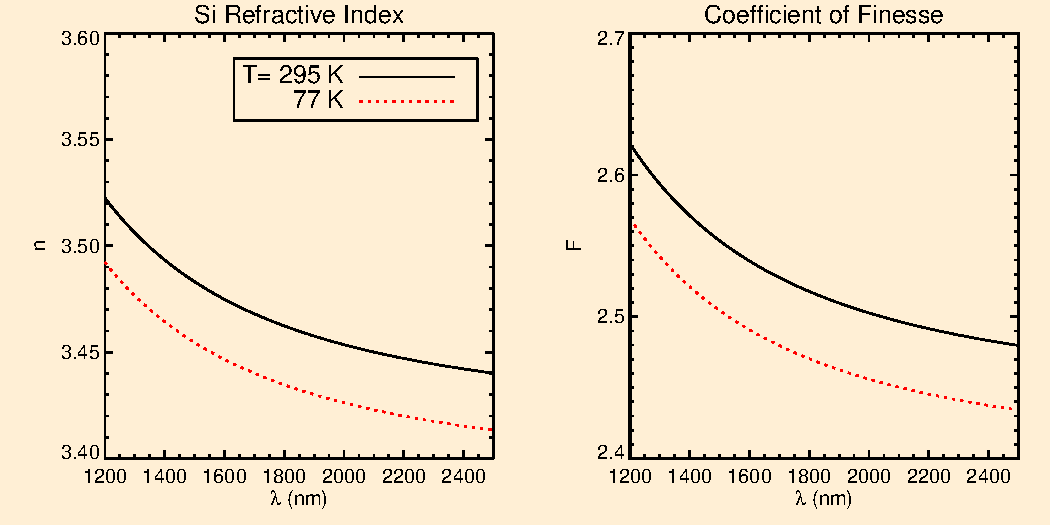
\includegraphics[width=0.95\columnwidth]{chSiGaps/figs/SiIndexAOmgsFinesseFig.pdf}
\caption{Plot of refractive index, $n$, and coefficient of finesse, $F$, as a function of wavelength, $\lambda$.\label{figSiIndexFinesse} We computed the temperature dependent refractive index from the tabulations of \cite{2006SPIE.6273E..77F}.  The coefficient of finesse is defined in Equation \ref{eq:FabPerot}.}
\end{figure}

We can treat a small Si$-$Si interface gap between two almost-bonded silicon parts as a low-Finesse Fabry-P\`{e}rot etalon\cite{2007fuph.book.....S}.  The key property of an etalon is that it has a cavity enclosed between two smooth and parallel reflective surfaces where the requirements for smoothness and parallelism depend on the reflective finesse of the cavity.  For the narrow air gaps we consider here and for the modest reflectivity of a Si-vacuum interface, most gaps at Si$-$Si bonds will form effective etalons over most of their area.  The transmission through a Fabry-P\`{e}rot depends on the wavelength of light, the reflectivity of the etalon sidewalls, and the size of the gap.  We compute the reflectivity for an Si$-$vacuum interface, which is a modest function of wavelength through the refractive index of Silicon, $n(\lambda, T)$ \cite{2006SPIE.6273E..77F}, as shown in Figure \ref{figSiIndexFinesse}.  We drop the subscripts on the refractive index $n(\lambda, T) \rightarrow n$ and the coefficient of finesse $F(\lambda, T) \rightarrow F$ for clarity.  The computation is simply Fresnel's law at normal incidence:

\begin{eqnarray}
R = \frac{(n-1)^2}{(n+1)^2} \label{Eq:FresnelR}\\
F \equiv \frac{4R}{(1-R)^2} \label{Eq:coeffF}
\end{eqnarray}

We define the coefficient of finesse\cite{2007fuph.book.....S}, $F$ (Equation \ref{Eq:coeffF}), in the customary way to encapsulate the Fabry-P\`{e}rot etalon's dependence on reflectivity.  The right panel of Figure \ref{figSiIndexFinesse} shows the coefficient of finesse as a function of wavelength.  In this work, we assume transmission is at normal incidence and the refractive index of the gap is 1.0.  Si absorbs negligibly longward of $\lambda$ = 1250 nm, which we verified by comparing the transmission of Si reference samples of different thicknesses (Figure \ref{figSiAbsorbfig}).  We measured the ratio of transmissions of a 0.5 mm thick double side polished Si wafer and a 3.0 mm Si puck.  Figure \ref{figSiAbsorbfig} verifies a key assumption that we make when comparing the transmission of scrap Si of different provenance and thickness.  Specifically, double side polished 3 mm thick Si pucks and 0.5 mm thick Si wafers have indistinguishable transmission at the $<0.2$\% level long-ward of $1250\;$nm.  The Si refractive index is indistinguishable from sample to sample for the wavelength ranges we care about- the non-absorbing wavelengths greater than about 1250 nm.  \cite{2006SPIE.6273E..77F} cites the wide variety of values for refractive index from the literature as evidence that batch-specific Si should be used as a reference for cases in which absolute accuracy greater than $\pm5\times10^{-3}$ is desired.  An absolute deviation of $\pm5\times10^{-3}$ in refractive index corresponds to a Fresnel transmission difference of about 0.2\%, which is comparable to our measurement uncertainty.  In the next subsection we work out the wavelength dependent transmission for the air etalon\footnote{A note on nomenclature- we use the term \emph{gap} for the physical structure, and \emph{etalon} for the model of that structure.}

\begin{figure}[htbp]
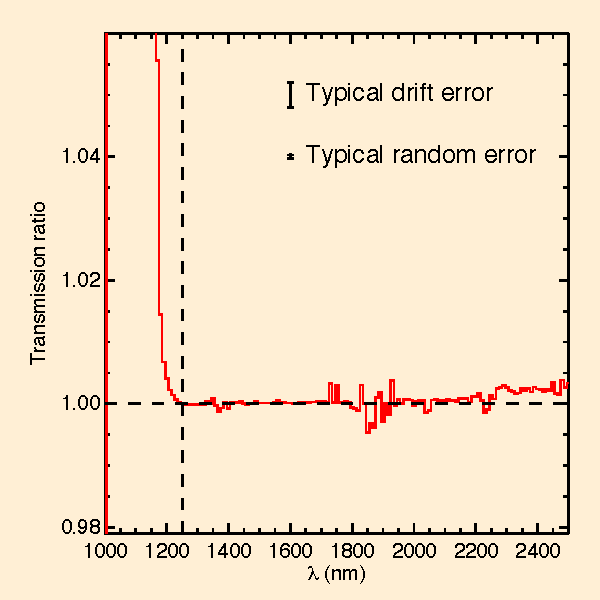
\includegraphics[width=0.40\columnwidth]{chSiGaps/figs/fpAbsorbfig_alt}
\caption{Ratio of transmission of a 0.5 mm thick Si wafer to that of a 3.0 mm thick Si puck.  \label{figSiAbsorbfig} We detect Si absorption shortward of $\lambda$ = 1250 nm.  The individual measurements have correlated uncertainties attributable to lamp drift at the level of 0.2\%.  The random uncertainties are typically about 0.02\% per sample, though some wavelength regions (e.g. 1700-1900 nm) demonstrate much greater per sample uncertainties.  Absorption longward of 1250 nm (vertical dashed line) is negligible.}
\end{figure}

\subsection{Predicted transmission spectrum for bonded Si with finite interface gap}
\label{secTheory}
A pair of bonded silicon wafers or pucks with a small gap forms three coupled cavities with the air gap as the the central cavity.  The outer cavities, those within the Si, however, were not produced with coherence in mind.  Their sides are not necessarily flat and parallel to the required level and the specifics of their deviation from perfect etalons are usually not known to the level necessary to treat them as coherent structures in the analysis.  The multiple internal reflections within the Si therefore present a hurdle to an analysis of the air gaps.  In the air gap, however, the gap size is small enough that the cavity it forms can always be treated as a coherent structure.  Treatments for multiple coherent reflections have been described in detail in the optics literature \cite{2007fuph.book.....S}.  The wave transfer matrix technique treats each dielectric interface as a matrix with elements relating the pre- and post- interface complex amplitudes in the left and right directions.  We adapted the wave transfer technique for incoherent interactions \cite{2002ApOpt..41.3978K} to deal with the cavities within the thick Si substrates.  Specifically we constructed an incoherent wave transfer matrix whose elements relate the intensities (and not complex amplitudes) before and after an interface.  The details appear in Appendix \ref{sec:Append-IMRTMM}.  We computed the transmission for two scenarios: first a double side polished (DSP) Si sample with no gap, and second a pair of bonded Si samples with a gap thickness $d$.  The DSP Si sample with no air gap has a transmission equal to:

\begin{eqnarray}
T_{DSP} = \frac{2n}{1+n^2} \label{eqnAbsDSPtrans}
\end{eqnarray}

which has an average value of about 53\%.  Note that this transmission is above a na\"ive value of $T_{DSP}=(1-R^2)$, which does not take into account multiple incoherent reflections, and is therefore an underestimate.  The top line in the upper panel of Figure \ref{figAbsoluteTrans} shows the value derived from Equation \ref{eqnAbsDSPtrans} in the wavelength range $1200-2500\;$nm.  If the Si substrate thickness is less than the coherence length for the given spectral bandwidth, and if its surface roughness is much smaller than the wavelength, our assumptions break down and the multiple reflections would interfere coherently, and the outer Si cavities would behave as a Fabry-P\`erot etalon.  We do not treat this case here since our focus is on thick substrates with small gaps between the interfaces.


\begin{figure}[!htbp]
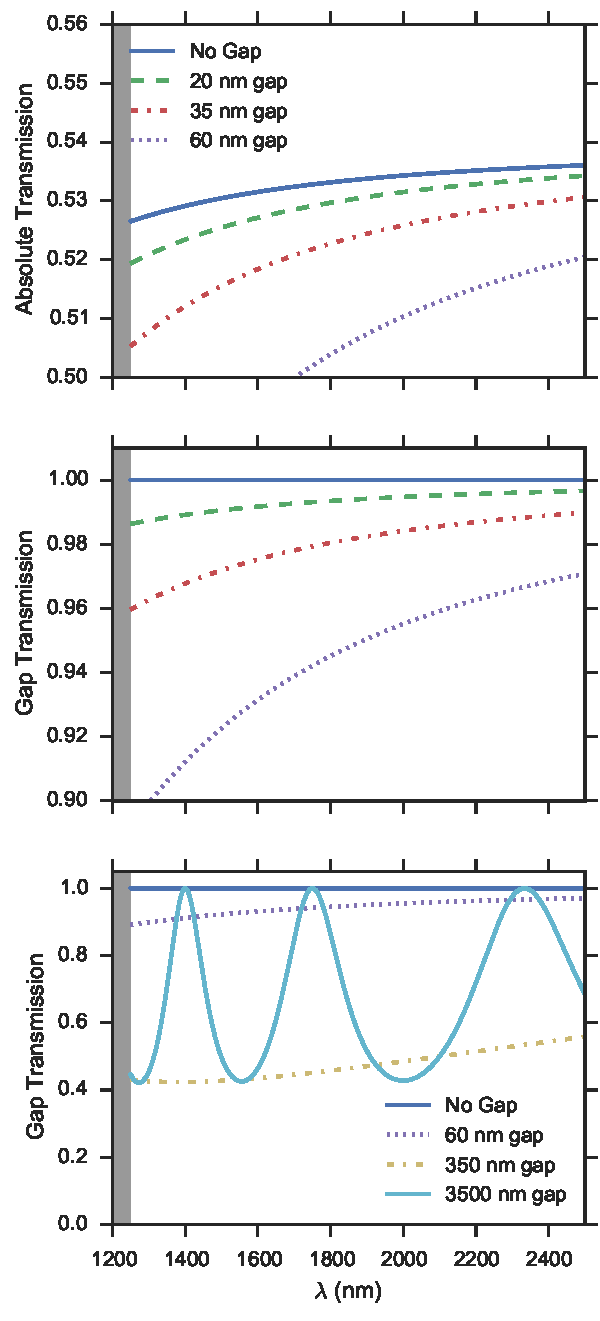
\includegraphics[width=0.40\columnwidth]{chSiGaps/figs/etalon_trans.pdf}
\caption{\label{figAbsoluteTrans}The family of normal-incidence curves for transmission as a function of wavelength for various gap sizes in bonded Si optics.  \emph{Top panel}: Absolute transmission through a Si substrate with no gap (top denim-blue solid curve), and small gaps of axial extent 20 nm (green dashed curve), 35 nm (red dash-dotted curve), and 60 nm (purple dotted curve).  The absolute transmission through Si depends on wavelength since the refractive index depends minutely on wavelength.  The curves assume that multiple reflections within the Si substrates add incoherently as discussed in detail in Appendix \ref{sec:Append-IMRTMM}.  \emph{Middle panel}: The ``Gap Transmission'', defined as the Absolute transmission through a sample normalized by the absolute transmission through a gapless sample. The gap sizes and colors are the same as in the top panel.  \emph{Bottom panel}: ``Gap Transmission'' for larger gaps, spanning 0-3500 nm.  The 3500 nm sized gap (cyan solid line), demonstrates characteristic Fabry-P\`erot etalon fringes.}
\end{figure}

Consider a pair of bonded Si samples with a gap thickness $d$. We derive the absolute transmission of bonded Si substrates with a gap in Equation \ref{eqn:Tetalon} in the Appendix.  We normalize the absolute transmission by the transmission of a double-sided Si structure with no gap to isolate the effect of the gap.  We call this normalized transmission the gap transmission $T_{g}$.

\begin{eqnarray}
T_{g} = \frac{n^2+1}{2 n F \sin ^2(2\pi \frac{d}{\lambda})+n^2+1} \label{eqFP}
\end{eqnarray}

In the limit $\lim_{d \to 0} T_g \rightarrow T_{DSP} $ and the gap approaches 100\% transmission.  Figure \ref{figAbsoluteTrans} shows a plot of Equation \ref{eqFP} for gap sizes, $d$, of 0, 20, 35, 60, 350, and 3500 nm.  The bottom two panels show the ``gap'' transmission based on Equation \ref{eqFP}, the value of the throughput with the losses from the outer Si cavities divided out.  For the very largest gap, large fringes appear as the cavity resonance of the air gap modulates the transmission.  Below a $\lambda/2$ gap size, the gap manifests itself as a wavelength-dependent diminution of the transmission.  For the smallest ($35-60$ nm) gaps, there is a $2-6\%$ decrease in gap transmission from $2400\;$nm down to $1250\;$nm.  It is the magnitude and wavelength dependence of this transmission spectrum that provides information about the axial extent of the gap.

\section{Laboratory demonstration: Embedding gaps of known sizes}

We evaluated our metrology method by embedding gaps of known sizes in the interface between two bonded Si substrates and measuring the effects of these gaps on IR transmission.  The substrate thicknesses ranged from 0.5 to 3.3 mm.  We denote substrates with thicknesses larger than 1 mm as ``pucks'' and substrates with thickness less than 1.0 mm thick as ``wafers''.  We distinguish the two classes of substrate thickness based on the anticipation that thin substrates will conform more easily to their bonding partner substrates.  There is also evidence that bond front propagation is slower in thick pucks \cite{2007ApOpt..46.6793H} than in wafers.  Our ultimate goal is to bond optics with thicknesses as large as 30 mm.

The three important characteristics of gaps are their axial extent, their lateral areal extent, and the areal fill factor of ensembles of such gaps.  To fabricate our test samples, we used photoresist lithography to pattern Si substrates, and we bored holes with inductively coupled plasma etching.  We used two different gases with low and high etch rates, CHF$_3$ on Si exhibited about 0.3 nm/second etch rate, SF$_6$ exhibited about 1 $\mu$m/minute to produce gaps with small and large depths.  Tables \ref{tbl_experiments} and \ref{tbl_meshPatterns} give information about the hole patterns and depths, as measured with Veeco NT9100 Optical Profiler for the small depth, and Dektak stylus profilometry for the large depth.

The fill factor is the pattern area covered by gaps relative to the total pattern area.  We achieved gap sizes of $14-95\;$nm on four substrates with three meshes with coarse, medium, and fine boxes, each with 50\% fill factors.  We did not verify the delivered fill factor, but since high precision lithography is very reliable, we assign no uncertainty to the difference between the delivered fill factor and the designed fill factor.  For measurements taken with the Veeco NT9100 Optical Profiler, uncertainties were constructed by inspecting the histogram of topology, as shown in Figure \ref{figVS20pattern}.  The large-scale distortions were removed from the topology by masking and flattening to ensure that the uncertainties accurately reflect the distribution of measured heights.  The stylus profilometry measured values were assigned an uncertainty of 5\%, our experience with other etched parts.  Table \ref{tbl_experiments} lists part numbers and descriptions for our bonded substrates.

\begin{figure}[htbp]
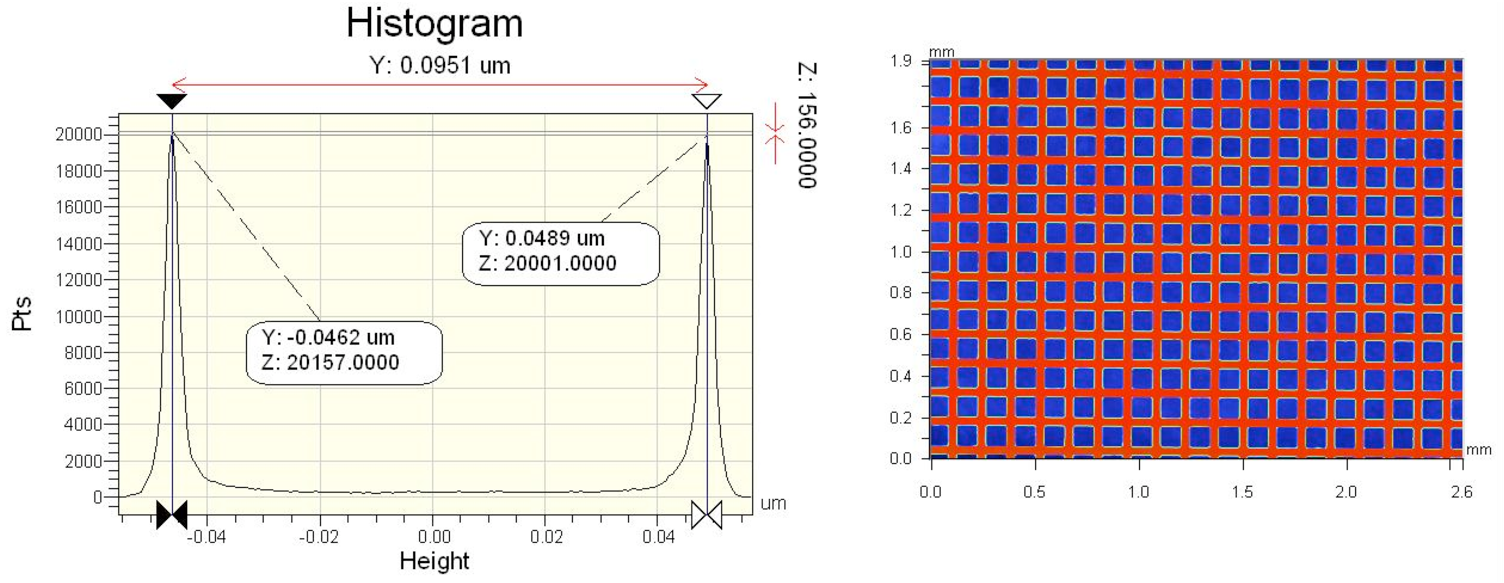
\includegraphics[width=1.0\columnwidth]{chSiGaps/figs/VS20fineGapCrop.pdf}
\caption{
\label{figVS20pattern}
Veeco optical profiler surface plot and histogram for part VS20-21 in the fine pattern section.  The 100 mm diameter VS20-21 is comprised of two thick silicon wafers.  We patterned three meshes with coarse, medium, and fine boxes, each with 50\% fill factors.  The depth was $95 \pm 5\;$nm as indicated by the well-separated peaks in the Veeco profilometry histogram.  The fill factor for this and all mesh patterns was 50\%.  The purpose for these patterns was to have gaps of known axial extent against which we could test the optical metrology technique we describe in this article.}
\end{figure}

\begin{table}[h!]
\caption{UTexas Si bonding experiments \label{tbl_experiments}}
\begin{center}
    \begin{tabular}{ c c c c c}
    \hline
    Name & Diameter & Thickness & Pattern & Pattern Depth\\ 
    -  & mm & mm & - & nm \\
        \hline
    VG02   & 100 & 3.3 $\times$ 2 &  None  & - \\
    VG03   & 100 & 3.3 $\times$ 2 &  Hole \& Petal & 4000$\pm$200 \\
    VG09-12   & 75   & 1 $\times$ 2 & Mesh C & 49 $\pm$6 \\
    VS20-21   & 100 & 0.8 $\times$ 2 &  Mesh C, M, F & 95 $\pm$5 \\
    \hline
    \end{tabular}
\end{center}
\end{table}

\begin{table}[h!]
\caption{Patterned gap properties \label{tbl_meshPatterns}}
\begin{center}
    \begin{tabular}{ c c c c }
    \hline
    Pattern & Fill Factor & feature size & bulk description \\ 
    - & \% & $\mu$m & - \\ 
    \hline
    Hole   & 100     &  -         & 25 mm diameter hole \\     
    Petal  & $\sim5$ & $\sim$2000 & 2 mm wide lines \\         
    Mesh F & 50      &         40 & 100 $\mu$m square holes, Fig. \ref{figVS20pattern}\\ 
    Mesh M & 50      & 200        & 500 $\mu$m square holes\\ 
    Mesh C & 50      & 620        & 1500 $\mu$m square holes\\     
        \hline
    \end{tabular}
\end{center}
\end{table}

We cleaned the surfaces before bonding to minimize the interfacial particle density.  The surface roughness was typically about 2 nm, as measured with a Veeco NT9100 Optical Profiler.  We also measured the large scale surface flatness of the pucks.  The Fisba2 interferometer used for these measurements has a 50 mm diameter beam at $\lambda=632.8\;$nm.  We found a typical peak to valley surface flatness of 2 waves over the central 50 mm diameter.  We prepared the substrates with standard cleaning procedures of solvents in a megasonic.  We then applied MHz frequency oxygen plasma ashing.  We soaked the wafers in DI water then dried with N$_2$.  We pressed the Si substrates together from the center to the outside.

\subsection{IR bubble imaging and limitations}

We first looked for large gaps in our bonded substrate pairs detectable as ``IR bubbles'' \cite{1992JEMat..21..669M}, with IR imaging.  The detector was an IR Vista $\alpha$NIR infrared focal plane array, with 312 $\times$ 252 pixels, with 30 $\mu$m square pixels.  We used a 50 mm F/2 lens, with a fiber optic white light illumination source.  The combination of the absorption of Si, the lamp spectrum and the detector responsivity led to an effective bandpass from approximately $1.15-1.6\;\mu$m.  The field of view was smaller than the 100 mm diameter wafers, so we dithered the sample.  Figure \ref{figVS2021_IR_image} shows an IR image of bonded sample VS20-21.  For this image, we coarsely flat-fielded the detector by observing a homogeneously illuminated white screen. Despite the flat-fielding, detector non-uniformities and vignetting are perceptible in our image as vertical stripes.  Mosaic-stitching errors are also perceptible.  It was easy to detect IR bubbles despite detector artifacts since the bubbles translate with the sample when we dither its position.

We also used IR imaging to inspect VG09-12 and VG15-13.  We detected IR bubbles in all 3 of these bonded Si samples.  The observable bubble areal density varied from about 4 per 100 mm diameter bonded wafer pair to over 20 per bonded wafer pair.  The individual IR bubble areas were as small as a few square millimeters up to $400\;\mathrm{mm}^2$.  The IR bubbles had various morphologies.  The structure within some of the images of IR bubbles showed Newton's rings, exposing the presence of gaps larger than about $\lambda/2$ up to $\sim 15 \lambda$.  As expected, the unbonded DSP wafers show no such IR bubbles.  No attempt at quantitative measurement was made on the IR images due to evidence of a non-linear detector response.  The bulk morphologies were clear regardless of the detector response.  When IR imaging was available, it was leveraged to target IR spectroscopy in locations demonstrating presence or absense of IR bubbles, as desired.  In other cases when IR imaging was not available or ignored, spectra were taken at random positions on the wafer.

\begin{figure}[htbp]
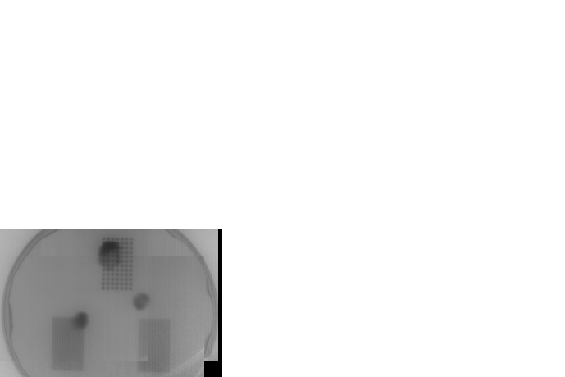
\includegraphics[width=0.4\columnwidth]{chSiGaps/figs/VS2021_IR_image.pdf}
\caption{
\label{figVS2021_IR_image}
IR image of part VS20-21. Three rectangular mesh areas are apparent (Table \ref{tbl_meshPatterns}).  The coarsest mesh, C, shows substructure, while the medium and fine meshes are indistinguishable at the low resolution of the image.  The three dark spots are gaps at the interface of the direct bonded Si samples.}
\end{figure}


\section{Measurement technique and correlated measurement errors}
\label{sec_aboutErrors}

We used the test pieces with known gaps to validate our measurement and analysis techniques.  We took transmission spectra of the bonded Si wafers and pucks, and the double side polished Si reference wafers using an Agilent Cary 5000 UV-Vis-NIR spectrophotometer.  Table \ref{tabCary5000pars} lists the typical measurement settings and tool performance.  The tool has a double monochromator, which reduces scattered light.  The vendor reported linearity exceeds 40 dB.

The Cary 5000 has four operation modes: single front, single back, double, and double reverse.  Double mode takes a reference spectrum simultaneously with the target spectrum.  We experimented with single front and double modes.  In principle double beam mode is even more precise than single beam mode.  In practice we found that souble beam mode showed evidence for lamp-jump artifacts attributable to polarization differences between the two arms.  So in this article we focus our results to those obtained in single beam mode.  In both single and double mode, the spectrometer takes a baseline scan with no sample in the measurement holder.  We automatically divide sample spectra by this baseline spectrum.  In single beam mode, we must repeat the baseline measurements about every 10-30 minutes for post-process division.

We estimated the uncertainty and measurement repeatability experimentally.  We computed the RMS error and measurement repeatability in a single measurement by computing the standard deviation of a spectrum taken immediately after a baseline scan with no sample present.  We found that the mean value in single mode drifted by about 0.2\% over several measurements.  The standard deviation of the featureless spectrum was typically 0.02\% from point to point, with some portions of the spectrum demonstrating increased variance.  Table \ref{tabCary5000pars} summarizes the amplitudes of the drifts and individual measurement errors.  \emph{Correlated errors dominate the measurement uncertainty of our transmission spectra.}  The measurement uncertainty correlations are apparent in Figure \ref{figSiAbsorbfig}.  In some parts of the spectrum, the mean drift is about ten times larger than the local standard deviation of the spectrum.

The spectral sampling ranged from 2.0 to 10.0 nm.  We set the spectrometer slit width to produce a spectral resolution of 5.0 nm.  We expect smoothly varying spectral features for all conceivable interface gaps in Si bonded wafers.  Specifically, Fabry-P\`erot fringes attributable to interfacial gaps in bonded Si will be well-sampled with 5 nm spectral resolution, so long as the interface gap is less than $\sim$100 $\mu$m.  This maximum gap limitation brings our technique to the point where it overlaps in capability with other techniques since the axial extents of such large gaps would be easily measurable by other means, like IR imaging and fringe-counting.

We also verified the linearity of the detector response my measuring the transmission through stacks of filters.  We constrained the linearity to at least $>24$ dB.  The vendor reports linearity exceeding 40 dB, which is consistent with our measurement.  

\begin{table}[h!]
\caption{Summary of Cary 5000 Measurement parameters \label{tabCary5000pars}}
\begin{center}
\begin{tabular}{ c c }
\hline
        Parameter (Units) & Value \\ 
\hline
        Spectral sampling interval (nm) & 2.0,10.0 \\
        Spectral resolution (nm) & 5 \\
        Time per sample (s) & 0.1 \\
        Typical measurement range (nm) & 1200-2500 \\
		Typical Single mode mean drift (\%) & 0.20 \\
		Typical Single mode standard deviation (\%) & 0.02 \\
 		Beam size (mm $\times$ mm) & $2 \times 8$ \\
        Directly measured linearity range (dB) & $>24$ \\
    \hline
    \end{tabular}
\end{center}
\end{table}


\section{Results of infrared spectroscopy of directly bonded Si}
\label{secResults}

The gaps in our test pairs should be a combination of the deliberately induced gaps and any inadvertent additional spaces caused by imperfections in the bonds.  We infer the axial extent of gaps in our samples with etched holes from their measured transmission spectra.  We use a Bayesian inference technique in our analysis.  First we define a mixture model in which the observed normalized gap spectrum $T_{obs}$ is composed of a sum of a spectrum through a gap of axial extent $d$, and a spectrum through a perfect bond:

\begin{equation}
	T_{mix} = f\;T_{g} + (1-f) \label{eqnMix}
\end{equation}

where $f$ is the areal fill factor of the region exhibiting a finite gap size, and $1-f$ is therefore the areal fill factor of the perfectly bonded area.  $T_g$ is defined in Equation \ref{eqFP}.  The only free parameters in Equation \ref{eqnMix} are $d$ and $f$.  Both of these parameters are fixed in our direct bonded Si wafers with synthetic gaps, and are listed in Table \ref{tbl_meshPatterns}.  These synthetic imbedded gaps therefore offer an excellent test of our ability to recover the gap axial extent $d$ and areal fill factor $f$ (Section \ref{secKnownGaps}).

Equipped with an observed spectrum and our mixture model, we constructed the likelihood function \cite{2013sdmm.book.....I}.  The measurement errors are strongly correlated as discussed in Section \ref{sec_aboutErrors}.  To handle the correlated measurement errors we use Gaussian process regression \cite{rasmussen2006gaussian, DFMgp}.  The Gaussian process takes into account the unknown but finite covariance structure by introducing a covariance matrix, $\boldsymbol{C}$ whose elements represent the correlations of each sample $i$ with every other sample $j$.  We parameterize the covariance matrix elements in the following way:

\begin{equation}
	C_{ij} = \sigma^2_{i}\delta_{ij}+a^2\exp{(-\frac{(\lambda_i-\lambda_j)^2}{2s^2})} \label{eqnGPkernel}
\end{equation}

where $\delta_{ij}$ is the Kronecker delta, and $\sigma_i$ are the independent measurement uncertainties on the $i^{\mathrm{th}}$ data point. The parameter $s$ controls the correlation length, and $a$ controls the amplitude of the correlated noise.  We experimented with different values for $\sigma_i$.  When repeated double side polished reference sample measurements were available, we estimated the $\sigma_i$ from the dispersion around mean-subtracted, detrended transmission spectra.  We do not know $a$ nor $s$ and they are, in general, different for each measurement-- they are \emph{nuisance parameters}, and are ultimately marginalized out.  They arise from the uninteresting properties of the spectrometer, and their interpretation is immaterial.  The value of $a$ should be close to the mean drift reported in Table \ref{tabCary5000pars}.  The value of $s$ could be small (tens of nm) to capture local variation attributable to atmospheric air absorption, or large (hundreds or thousands of nm) to capture global features attributable to lamp drift.  We allow both $a$ and $s$ to be free parameters in our fitting procedure.

We set our prior probability distribution functions \cite{2013sdmm.book.....I}, $\ln{p(d,f,a,s)}$ as uniform over a wide range of values for $\ln{a}$, $\ln{s}$, $d$, and $f$, consistent with visual inspection of each spectrum.  The final un-normalized posterior probability function, expressed as a natural logarithm is:

\begin{equation}
	\ln{p(d,f,a,s|\lambda, T_{obs}, \sigma_i)} \propto \ln{p(d,f,a,s)} -\frac{1}{2}\;\boldsymbol{r^\intercal}\boldsymbol{C^{-1}}\boldsymbol{r} -\frac{1}{2}\;\ln{\det{\boldsymbol{C}}} \label{eqnPosterior}
\end{equation}

where the residual vector $\boldsymbol{r}$ is the data $T_{obs}$ minus the model $T_{mix}$.  We produce posterior samples with Markov Chain Monte Carlo (MCMC).  Specifically, we implemented \texttt{emcee}\footnote{\url{https://github.com/dfm/emcee}}\cite{emcee}, with 32 walkers, hundreds of burn-in samples, and 600-1000 iterations.  We initialized the walkers in the vicinity of our best guess for parameters based on visual inspection of the spectra.  Figures \ref{figVG03full}, \ref{figVG03part}, and \ref{figVG12} show examples of posterior samples including corner plots of the interesting physical parameters $d$ and $f$.

\subsection{Spectra of direct bonded Si with known gap sizes}
\label{secKnownGaps}

Figure \ref{figVG03full} shows a parameter determination for the measurement of a bond over a deep ($4000 \pm 200\;$nm) 100\% fill factor gap in part VG03.  The analysis yields a best fit consistent with 100\% fill factor, and a depth of $3960 \pm 2\;$nm, well within the uncertainty of the physical measurement (Table \ref{tbl_experiments}).  The spectrum in this region shows characteristic Fabry-P\`erot fringes of constructive and destructive interference.  The only tunable parameters of the model are the gap axial extent, $d$ and fill factor $f$.  No scaling has been applied to the curves in Figure \ref{figVG03full}.  Figure \ref{figVG03part} shows a fit for a region of the same bonded pair where a nominally $4000\;$nm deep, 2 mm wide trench crosses the field scanned by the Cary 5000.  Analysis of this transmission curve gave a best fit depth of $4094 \pm 4\;$nm and a pattern fill factor of $4.6 \pm 0.1\;\%$, both consistent with the part geometry.  These two results show that the formalism performs as expected on resonant gaps several wavelengths deep.

\begin{table}[h!]
\caption{Inferred Gap sizes and fill factors \label{tbl_DerivedGapSizes}}
\begin{center}
    \begin{tabular}{ c c c c c }
    \hline
    Name & Region & Predicted $d$ & Measured $d$ & $f$ \\
    -  & - & nm & nm & - \\
    \hline
    DSP & -    &   0.0  & $3^{+8}_{-2}$ & $0.260^{+0.456}_{-0.230}$\\
    VG09-12 & Off-Mesh    &   0.0  & $11^{+21}_{-7}$ & $0.25^{+0.46}_{-0.22}$\\
    VG03 & Hole    &   4000 $\pm$ 200  & $3960^{+2}_{-2}$ &  $0.999^{+0.001}_{-0.002}$\\
    VG03 & Petal   &   4000 $\pm$ 200  & $4094^{+4}_{-4}$ &  $0.046^{+0.001}_{-0.001}$\\
    \hline
    \end{tabular}
\end{center}
\end{table}

\begin{figure}[htbp]
        \centering
        \begin{subfigure}[b]{0.5\textwidth}
              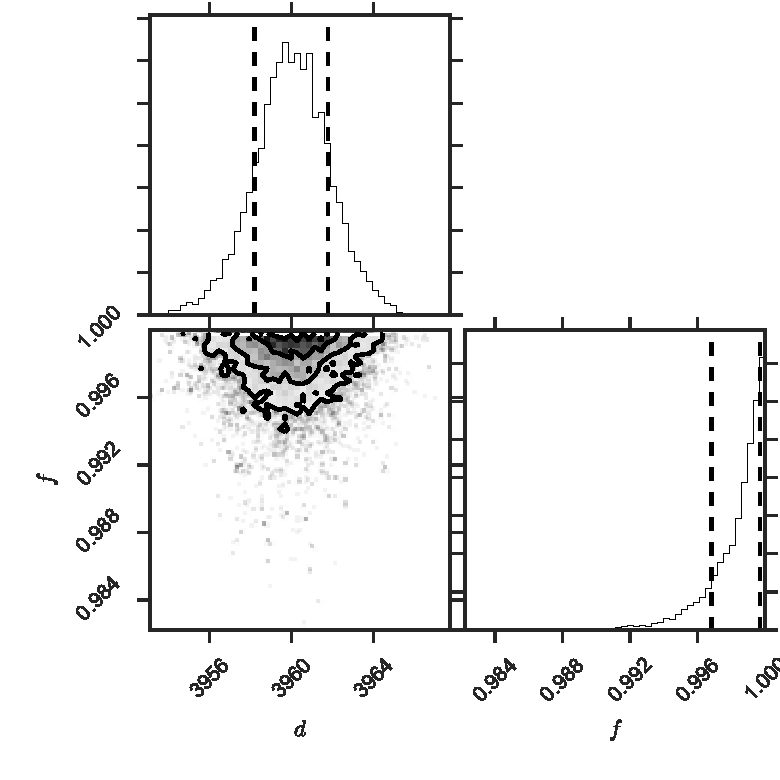
\includegraphics[width=\textwidth]{chSiGaps/figs/VG03_corner.pdf}
              \caption{Fitted gap size $d$ and fill factor $f$ for VG03 hole region}
		\label{figVG03_corner}
        \end{subfigure}

        \begin{subfigure}[b]{0.5\textwidth}
                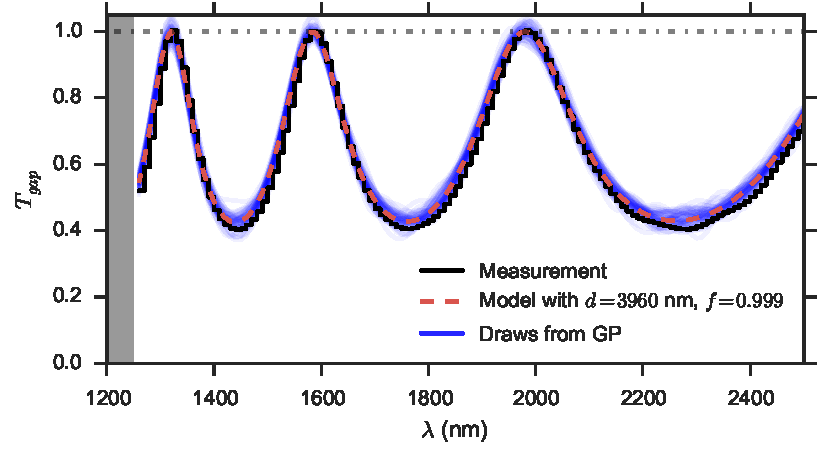
\includegraphics[width=\textwidth]{chSiGaps/figs/VG03_f100.pdf}
                \caption{Measured spectrum and fit of VG03 hole region}
                \label{figVG03_f100}
        \end{subfigure}
\caption{ \emph{Top panel:} Corner plot of MCMC samples in our non-linear model fit of the transmission spectrum of Si optic part \# VG03.  The physical parameters of the model are the axial extent of the gap $d$, and the areal fill factor $f$ of the gap over the measurement region.  The MCMC model fit also includes nuisance parameters $a$ and $s$ (not shown) for the Gaussian process covariance model.  \emph{Bottom panel:}Transmission through bonded Si sample VG03, normalized by the transmission of a DSP Si wafer. See the text for details on the sample, setup, and analysis.  The measured spectrum is the black stepped line.  The red dashed line shows the best model fit with $d$ = 3960 $\pm$ 2 nm, consistent with 100\% fill factor.  The blue band shows the collective locations of 60 random draws from the Gaussian process model.  Wavelengths short-ward of 1250 nm (gray band) were not included in the fit, since Si is absorptive there.\label{figVG03full} }
\end{figure}


\begin{figure}[htbp]
        \centering
        \begin{subfigure}[b]{0.5\textwidth}
              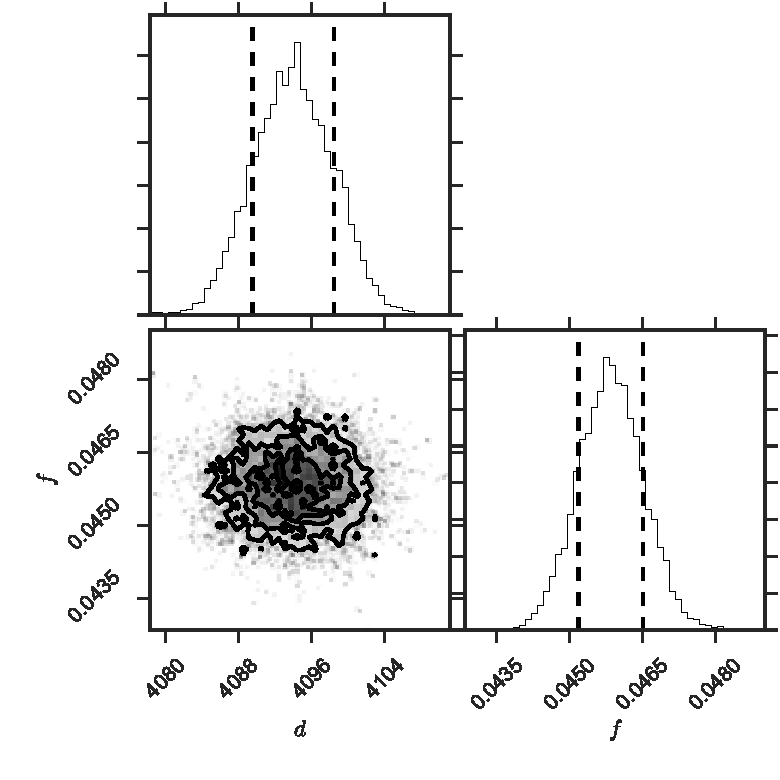
\includegraphics[width=\textwidth]{chSiGaps/figs/VG03p2_corner.pdf}
              \caption{Fitted gap size $d$ and fill factor $f$ for VG03 petal region}
		\label{figVG03p2_corner}
        \end{subfigure}

        \begin{subfigure}[b]{0.5\textwidth}
                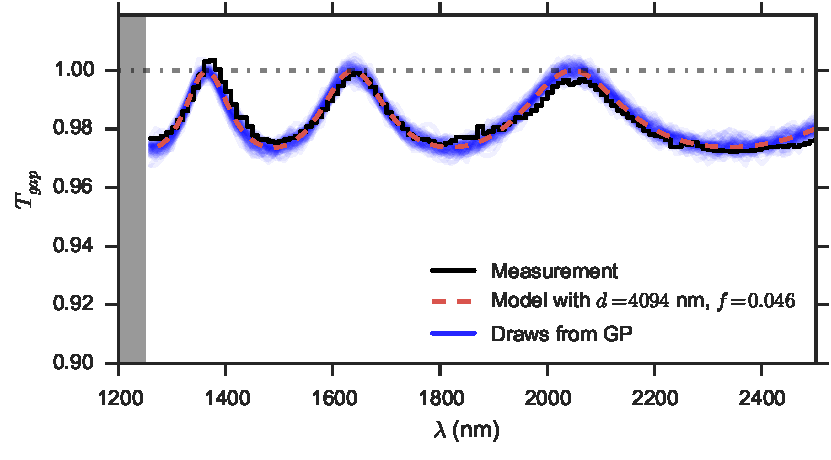
\includegraphics[width=\textwidth]{chSiGaps/figs/VG03_f045.pdf}
                \caption{Measured spectrum and fit of VG03 petal region}
                \label{figVG03_f045}
        \end{subfigure}
\caption{ Same as Figure \ref{figVG03full}, but the measurement was in a region where $<5\%$ of the area exhibited the $\sim4\; \mu$m gap.  The measured spectrum in this region shows subdued fringes. The model derived axial extent is 4094 $\pm$ 5 nm covering a fill factor of 4.58 $\pm$ 0.06$\%$. \label{figVG03part}}
\end{figure}


\subsection{Spatially resolved measurements with Sample Transport Accessory}
We acquired spatially resolved measurements of the pair of bonded parts VG09-12, (Tables \ref{tbl_experiments} and \ref{tbl_meshPatterns}) with the Cary 5000 sample transport accessory \footnote{\url{http://www.chem.agilent.com/en-US/products-services/instruments-systems/molecular-spectroscopy/sample-transport-accessory/}}.  This accessory translates the sample through the measurement beam and takes a transmission spectrum at each position.  We chose a 2 mm step size, which is slightly larger than the $\sim1$ mm beam width.  We sampled 50 mm across the mesh pattern and into the off-mesh pattern (Figure \ref{figVG0912_STA_illus}).  The large number of consecutive measurements prevented the requisite near-contemporaneous baseline measurements for normalization.  We fit a line to before-and-after baseline measurements to infer the mean-level drift, which we divided out of each spectrum.  We measured over a wavelength range from 1250 to 1775 nm.

The colored dots in the position marked in Figure \ref{figVG0912_STA_illus} match the color of the spectra in Figure \ref{figVG0912}.  The approximate size of the measurement beam is shown for scale.  The conspicuous mesh pattern has a depth of $49\pm6\;$nm, as measured with an optical profiler, and global fill factor of 50\%.  However, since the beam size is comparable to mesh grid size, the fill factor for any given measurement can vary from about 30\% to 75\%.  The gray band in Figure \ref{figVG0912} represents the allowable range of predictions, taking into account both the uncertainty in the mesh depth and fill factor.  If the mesh pattern were perfectly bonded, we would expect all the spectra to fall inside the color swath in Figure \ref{figVG0912}.  We see excellent consistency between prediction and measurement, with one measured spectrum hinting at a small gap ($\lesssim15$) in one measurement position.  Outside the mesh area, the bonding is excellent, as demonstrated by the off-mesh transmission with transmission consistent with 100\% to within the measurement uncertainty of 0.2\%.


\begin{figure}[htbp]
    \centering
    \begin{subfigure}[b]{0.35\textwidth}
        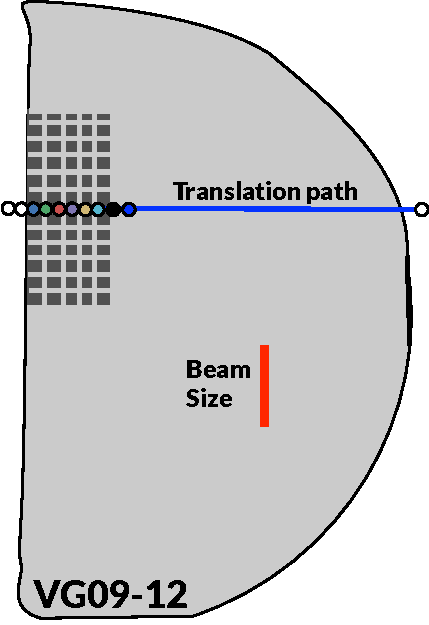
\includegraphics[width=\textwidth]{chSiGaps/figs/VG09_12_STA_illustration.pdf}
        \caption{Illustration of VG09-12 sample transport accessory measurement positions. \label{figVG0912_STA_illus} }
    \end{subfigure}
    \begin{subfigure}[b]{0.65\textwidth}
        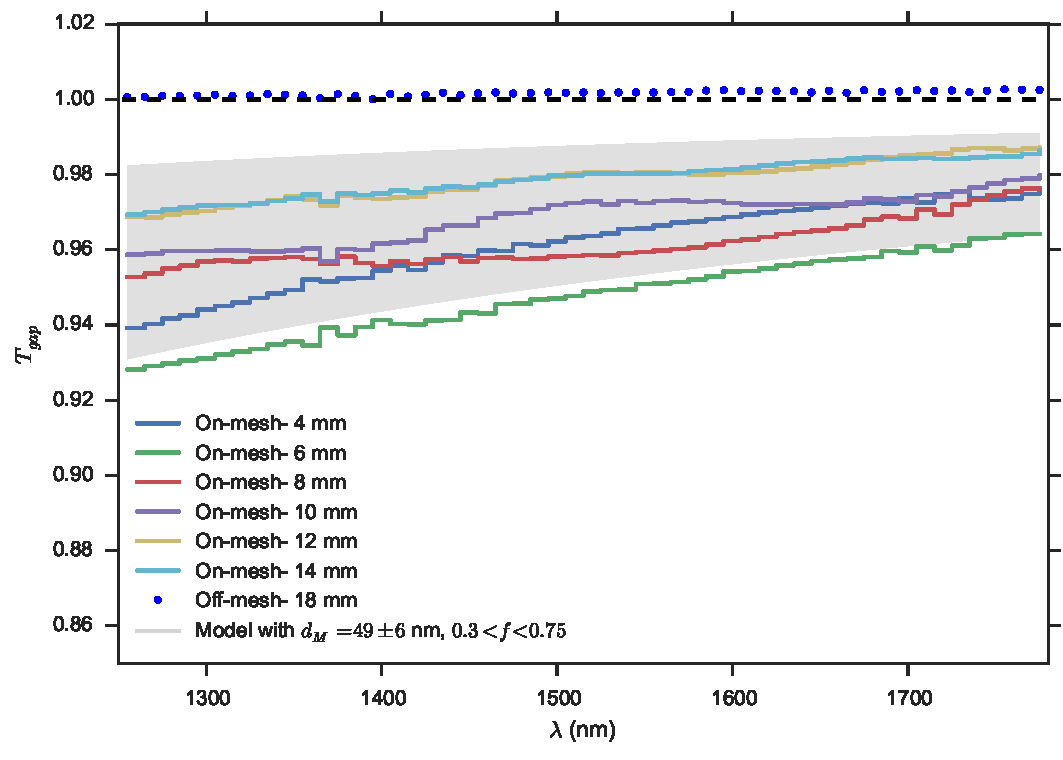
\includegraphics[width=\textwidth]{chSiGaps/figs/VG0912_STA_scan_coarse.pdf}
        \caption{Measured gap transmission spectra of VG09-12 on- and off- mesh \label{figVG0912}}
    \end{subfigure}
\caption{Predictions and measurements of the coarse mesh region in sample VG09-12.  We took 50 measurements across the face of VG09-12, including both on- and off- mesh regions.  The measurements are consistent with the predicted transmission, shown as the gray band.  The off-mesh regions demonstrate near-perfect bonding.\label{figVG12}}
\end{figure}

A key result of these test measurements is to demonstrate that gaps of known dimensions are recovered in our spectroscopy, both for large and small gaps.  Table \ref{tbl_DerivedGapSizes} summarizes the outcome of some measurements in the areas with known gaps and fill factors.  The table lists the median sample and 68\% confidence intervals.  The results from the scans shown in Figure \ref{figVG12} further support our conclusion.

\subsection{What is the smallest gap this technique can detect?}
We devised two experiments to approach the question, ``What is the smallest gap this technique can detect?''.  We applied our MCMC model fitting formalism to an unbonded DSP wafer.  The measured transmission spectrum was normalized by a transmission spectrum of the same sample taken only a few minutes earlier.  Any difference of this normalized transmission from unity is attributable entirely to measurement uncertainty, and represents the smallest possible signal one could extract.  We also measured bonded sample VG09-12 in a region away from the intentionally implanted gap.  This spectrum was processed in the same way as the spectra of the VG09-12 mesh area, exhibiting a mean value of 0.9998 and a standard deviation $\sigma=0.0008$.  This spectrum is consistent with no gap.  We applied our MCMC formalism to further constrain the range of gap sizes consistent with the spectrum.  Table \ref{tbl_DerivedGapSizes} summarizes the sizes of gaps.  The well-calibrated DSP noise spectrum rules out (at $>3\sigma$) gap sizes larger than about 9.0 nm over $>80$\% of the measurement area.  Similarly, the VG09-12 off-mesh spectrum rules out gaps greater than 14 nm over $>80$\% of the measurement area.  Figure \ref{figVG12} shows the corner plots and spectra for the off-mesh region in VG09-12.

\begin{figure}[htbp]
    \centering
    \begin{subfigure}[b]{0.5\textwidth}
        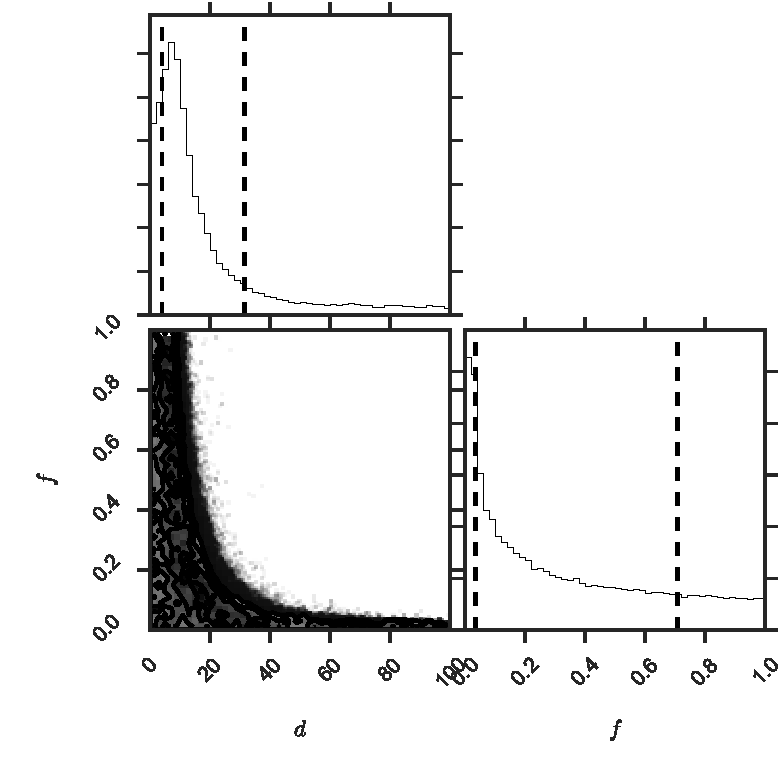
\includegraphics[width=\textwidth]{chSiGaps/figs/VG0912_0gap_corner.pdf}
        \caption{Fitted gap size $d$ and fill factor $f$ for VG09-12 off-mesh}
	\label{VG0912_0gap_corner}
    \end{subfigure}
    \begin{subfigure}[b]{0.5\textwidth}
        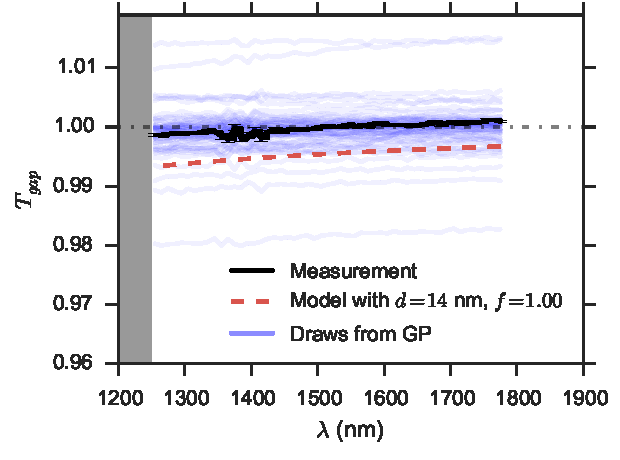
\includegraphics[width=\textwidth]{chSiGaps/figs/VG0912_0gap.pdf}
        \caption{Measured spectrum of VG09-12}
        \label{VG0912_0gap}
    \end{subfigure}
\caption{Similar to Figure \ref{figVG03full} and \ref{figVG03part}, but for sample VG09-12 in the off-mesh region.  The measured spectrum in this region shows no appreciable deficit of transmission from a DSP reference sample.
\label{figVG12}}
\end{figure}

Figure \ref{VG0912_0gap_corner} shows that there is a degeneracy between the axial extent of a gap and its fractional fill factor over the measurement beam; a larger gap can be hidden if it covers only a small fraction of the measured area.  The red dashed line shows the normalized transmission spectrum of a 14 nm gap over 100\% of the measurement area.  Gaps larger than 60 nm would have to cover less than 10\% of the measurement area in order to be consistent with the measurement.


\section{Discussion}

The experiments and measurements in Section \ref{secResults} demonstrate that we can detect and measure the axial extent of gaps down to 14 nm.  The technique is \emph{non-destructive} and can be implemented with an off-the-shelf commercial product, namely the Cary 5000 or equivalent, or any existing high precision spectrograph.  The spectrograph need not be high resolution-- our 5 nm spectral resolution was not a limiting factor.  The limiting factor is spectrophotometric \emph{accuracy} and \emph{precision}.  In this Section we question the assumptions of our technique, identify its limitations, and mention some opportunities.

\emph{More complex underlying gap size distributions-} One key assumption of our gap-as-etalon modeling strategy is that the distribution of gap sizes over the measurement area is bimodal- a gap of size $d$ or zero gap.  This choice was simply a matter of computational simplicity, and any more complicated gap size distribution could easily be dropped in as additional terms in Equation \ref{eqnMix}.  For example, if there is a gradient across the bond, the emergent transmission spectrum will be an admixture of many gaps with various areal coverage fractions.  The full solution becomes an areal integral of Equation \ref{eqFP} normalized by the total measurement area.  Solving for the relative distributions of gaps is highly degenerate, in the same way as we saw in the 2-parameter corner plots of gap depth and fill factor.  We experimented with by-eye fitting parametric distributions of gap sizes, characterized by a maximum and minimum gap size, and a monotonic slope of the distribution.  We found that measurements of very large ($>10\lambda$) gaps with a large gradient offered surprisingly strong constraints on the maximum gap size, because of the conspicuous high frequency Fabry-P\`erot fringes.  For sub-wavelength gaps, the gap size distribution is too degenerate to derive much useful insight on the slope of the distribution.  Specifically, for $d_{max}<\lambda/4$, our simple mixture model will converge on the spectrum of the average gap size, even if the \emph{True} distribution is more complex.  Reducing the measurement area could break some of these degeneracies, if more precision is desired.


\emph{The benefit of the Gaussian process-} We chose to estimate the gap size with a Gaussian process regression, but this is not necessary.  Any model fitting strategy, like least squares or over-plotting a model to data by-hand, will yield an estimate for a gap size.  We tested the benefit of Gaussian process regression by generating synthetic data spectra with known gap size and fill factor, and known covariance structure.  We applied ordinary least squares regression to the synthetic spectra and derived values for $d$ and $f$ that were biased by up to $20\sigma$ or more.  Applying Gaussian process regression recovered the input values to within $1\sigma$.

\emph{Normal incidence- } We have assumed that the transmission measurement is performed at normal incidence.  If the measurement beam forms a non-zero angle with the entrance face, bond interface, or exit face, several things happen to make this technique invalid.  Notably, the polarization effects, Fresnel reflection losses, and the incoherent multiple reflections change the emergent transmission spectrum in non-trivial ways.

\emph{DSP vs AR coated front faces- } We have assumed that the Si$-$air interfaces are approximated by Fresnel reflection losses.  If the entrance and exit faces of the bonded samples are AR coated, the incoherent multiple reflection model will have to be modified.  AR coated front and exit faces will result in a larger interface loss for a given gap size than the interface loss computed here.

\emph{How far can this technique go?}  The spectrophotometric precision of our instrument flows down directly to limit the smallest measureable gap size.  This limitation will vary from instrument to instrument.  Our instrument can achieve 10 times better accuracy and precision in double beam mode.  However, the slightly different polarization sensitivity in the different beams caused systematic jumps at the lamp/grating change-over wavelengths.  Agilent offers an adapter to reduce the polarization sensitivity, which mitigates these lamp jumps.  If precisions of 0.02\% could be achieved, gaps $<4$ nm could be reliably measured.  This level begins to be comparable to the effect of interesting physics, like surface roughness and refractive index.  In fact, the van der Waals bond energy could be constrained from these types of measurements \cite{2001JOptA...3...85G}.

\emph{Can this technique be applied to imaging?}  The analysis performed in this article informs smart strategies for using IR imaging for gap detection in bonded Si optics.  First, Equation \ref{eqFP} shows that short wavelengths have the most discerning power for detecting small gaps.  So an IR imaging approach should use the shortest possible wavelength without getting close to the Si absorption cutoff.  This work recommends a 1250$-$1300 nm filter.  Images can then be normalized to the transmission through a DSP sample under identical, nearly collimated lighting conditions.  Lastly, any deficits in flux of a bonded sample can be converted to a gap size $d$, using Equation \ref{eqFP}.  IR imaging will lack the spectral information available in the spectra shown in this article.  The imaging will require exceptional quality of flat-fielding or dithering of the images to reach the precision achieved here with relative ease.  

\section{Conclusions}
We have described a measurement technique and laid out an analysis formalism for the detection and measurement of sub-wavelength gaps at Si$-$Si interfaces.  Experimental measurements show that we can precisely recover the extent of wavelength-scale gaps of known size, account for the presence of small gaps, and capture results consistent with no gap when measuring a monolithic part.

The technique and formalism we describe here can detect and measure the axial extent of gaps in Si$-$Si optical bonds down to a level of $\sim14\;$nm.  It makes use of widely available off-the-shelf metrology equipment and simple to implement analysis.  Armed with this technique, optical fabricators have a new diagnostic tool to assess the quality of Si$-$Si bonds.



\section{Incoherent Multiple Reflections Transfer Matrix Method}
\label{sec:Append-IMRTMM}

Saleh and Teich (see Chapter 7 ``Fundamentals of Photonics'' \cite{2007fuph.book.....S}) describe the wave transfer matrix method.  Their technique is to assemble a 2$\times$2 scattering matrix $\boldsymbol{S}$ which has the elements:
\begin{eqnarray}
\boldsymbol{S} = \left(
\begin{array}{cc}
 t_{12} & r_{21} \\
 r_{12} & t_{21} \\
\end{array}
\right)
\end{eqnarray}
Where $t$ and $r$ stand for transmission and reflection respectively.  The order of subscripts is the order of origin and destination of the wave with respect to the interface, so we know the origin and direction of the wave.  The $\boldsymbol{S}$ matrix encapsulates all information about how light waves interact with the interface.  The power of the technique comes from the wave transfer matrix, $\boldsymbol{M}$.  The matrix $\boldsymbol{M}$ has the convenient property that its output can be used as the input for another matrix.  In other words, the input vector to $\boldsymbol{M}$ is made of the left and right moving components directly before the interface; the outputs are the left and right moving components directly after the interface:
\begin{eqnarray}
\left(
\begin{array}{c}
 U_2^{(+)} \\
 U_1^{(-)} \\
\end{array}
\right)=\boldsymbol{S} \left(
\begin{array}{c}
 U_1^{(+)} \\
 U_2^{(-)} \\
\end{array}
\right) \\
\left(
\begin{array}{c}
 U_2^{(+)} \\
 U_2^{(-)} \\
\end{array}
\right)=\boldsymbol{M} \left(
\begin{array}{c}
 U_1^{(+)} \\
 U_1^{(-)} \\
\end{array}
\right)
\end{eqnarray}

The elements of $\boldsymbol{S}$ and $\boldsymbol{M}$ are related to each other by geometric transformations\cite{2007fuph.book.....S}.  In thin films, the wavelength is comparable to the size of the dielectric layer and the vector components $U_{i}$ represent the complex amplitudes of the electromagnetic waves.  The polarization state can be encapsulated in scattering matrix components\cite{2007fuph.book.....S}.  The intensities of the emergent spectrum can be computed from the absolute square of the complex amplitudes.  For thick films, the vector components are the intensities of the emergent spectrum, since waves are incoherent.  \cite{2002ApOpt..41.3978K} work out the general transfer-matrix method for optical multilayer systems with incoherent interference.  The key idea for the incoherent transfer matrix method approach is to populate a scattering matrix with elements equal to the (wavelength dependent) transmitted $T_i$ and reflected $R_i$ intensities of an interface or set of interfaces that act together.  Then, use the geometric transformations to construct the $\boldsymbol{M}$ matrix.

The matrix for the silicon air gap is calculated in the following way.  We treat the air gap as a Fabry-P\`erot etalon.  We do not need to consider the microscopic coherent interactions with the etalon transmission, all of that information is encapsulated in these equations for a Fabry-P\`erot etalon model for the gap:

\begin{eqnarray}
 \delta = \frac{2\pi}{\lambda}2d \label{eq:phase} \\
  F \equiv \frac{4R}{(1-R)^2} \\
 T_g = \frac{1}{1+F\sin^2(\delta/2)}  \label{eq:FabPerot}
\end{eqnarray}

with $\lambda$ the vacuum wavelength, $R$ the Fresnel reflection of silicon, and $F$ the coefficient of finesse.  The coefficient of finesse $F$ and the phase $\delta$ are the two parameters of the Fabry-P\`erot etalon.  The coefficient of Finesse encapsulates the Fresnel reflection and depends only on the Si refractive index which has only a small wavelength (and temperature) dependence.  The phase depends (Equation \ref{eq:phase}) on the wavelength $\lambda$ and $d$ the air gap spacing.  We assume the gap is lossless, i.e. $T_g+R_g=1$.  So the incoherent scattering and transfer matrices for the gap are:

\begin{eqnarray}
\boldsymbol{S_g}&=&\frac{1}{1+F\sin^2{\delta/2}} \left(
\begin{array}{cc}
1 & F \sin ^2(\delta/2) \\
F \sin ^2(\delta/2) & 1 \\
\end{array}
\right) \nonumber \\
\nonumber \\
\boldsymbol{M_g}&=&\left(
\begin{array}{cc}
 1-F \sin ^2(\delta/2) & F \sin ^2(\delta/2) \\
 -F \sin ^2(\delta/2) & 1+F \sin ^2(\delta/2) \\
\end{array}
\right)
\label{eqn:EtalonMatrix}
\end{eqnarray}

We assembled the matrix for the Air-Si Fresnel interface at the exterior of the bonded Si parts in the following way.  First it is important to note that the matrix is the same whether the transmission is from Si to air or air to Si.  This reciprocity is not necessarily true for the complex amplitudes matrix, but our approach employs intensities not complex amplitudes.  The Fresnel interface is lossless.  The transmission and reflection are given by the Fresnel equation for normal incidence:
\begin{eqnarray}
T_n&=&\frac{4n_{Si}}{(n_{Si}+1)^2} \\
R_n&=&\frac{(n_{Si}-1)^2}{(n_{Si}+1)^2} \label{eq:FresnelTrans}
\end{eqnarray}
For clarity I will drop the subscripts from $n_{Si}$, since we have already set $n_{air}=1$ and there are no other dielectric interfaces to think about.  So the scattering and transfer matrices for the air-Si Fresnel boundary are:

\begin{eqnarray}
\boldsymbol{S_n}&=&\frac{1}{(n+1)^2} \left(
\begin{array}{cc}
4n & (n-1)^2 \\
(n-1)^2 & 4n \\
\end{array}
\right)  \nonumber \\
\nonumber \\
\boldsymbol{M_n}&=&\frac{1}{4n}\left(
\begin{array}{cc}
 -n^2+6  n-1 & ( n-1)^2 \\
 -( n-1)^2 & ( n+1)^2 \\
\end{array}
\right)
\label{eqn:SiAirMatrix}
\end{eqnarray}

Finally, we cascade the matrices together to compute the net transmission through the stack of abstractions.  The result is a $2\times2$ transfer matrix:

\begin{eqnarray}
\boldsymbol{M_{net}}=\boldsymbol{M_n}\boldsymbol{M_g}\boldsymbol{M_n}
\end{eqnarray}

From the matrix transformation equations \cite{2007fuph.book.....S} we know $M_{22}=1/T$.  Taking the inverse of the bottom right element of $\boldsymbol{M_{net}}$, we get the transmission $T_{net}$ through the net optical device:

\begin{eqnarray}
T_{net}=\frac{2 n}{1+ 2n F\sin ^2(\delta/2)+n^2} \label{eqn:FPmatTrans}
\end{eqnarray}

Compare equations \ref{eqn:FPmatTrans} and \ref{eq:FabPerot}.  The revised transmission has picked up a few factors of 2 and $n$.  While we are at it, let's compute the matrix for the scenario with no intermediate gap: there are simply two Fresnel interfaces with which light interacts incoherently.  This scenario is the model for a single DSP reference sample. The revised matrix multiplication is simply $\boldsymbol{M_{DSP}}=\boldsymbol{M_n}\boldsymbol{M_n}$.  Taking the inverse of the $M_{22}$ element, we find:

\begin{eqnarray}
T_{DSP}=\frac{2 n}{n^2+1}\label{eqn:EqofSummedSlab}
\end{eqnarray}

which is identical to the result obtained by directly summing the intensities from multiple reflections:
\begin{eqnarray}
T_{DSP}=T^2 \sum_{i=0}^{N}R^{2i} \label{eqn:multsum}
\end{eqnarray}

It is informative to isolate the effect of the gap by dividing the measured bonded wafer transmission by the transmission of a reference DSP Si part.  We call this normalized transmission the gap transmission $T_{g}$:
\begin{eqnarray}
T_{g} = T_{net}/T_{DSP} \\
T_{g} = \frac{n^2+1}{2 n F \sin ^2(\delta/2)+n^2+1} \label{eqn:Tetalon}
\end{eqnarray}



%\chapter{Immersion Grating Design Considerations}

\section{Blaze angle and choice of R}
Blaze angle choice is an important early design consideration for Si immersion gratings.  There is a dichotomy in choice- R1.4 or anything else\footnote{The R-number is the tangent of the blaze angle, and is often used for specifying the blaze angle of echelles for example ranges R1-R10  correspond to $\delta= 45-84.2\deg$}.  The choice of R1.4 simplifies the substrate preparation process because R1.4 ($\delta=54.7$) is the natural blazing provided by the Si (111) crystal plane (see Figure \ref{fig:Rnum}).  One can simply cut Si pucks from conventionally prepared Si boules, with the cuts on parallel planes to the top (100) surface of the Si boule.  Different blaze angles require an additional sample preparation step of x-ray orienting and precision cutting substrates at finite angles from the conventional (100) Si boule surface.  For example, an R3 grating has $\delta=71.6 \deg=54.7\deg+16.9$.  So, cutting the Si boule at 16.9$\deg$ will yield R3 blazed facets.  The cutting plane is normal to the major flat plane.  The middle pane of Figure \ref{fig:IGdesignplot} shows the cutting angle as a function of the blaze angle, with the width of the line equal to the uncertainty of the cutting angle associated with finite etching into the (111) Si crystal plane.  


\begin{figure}[h!] 
\begin{center}
\ 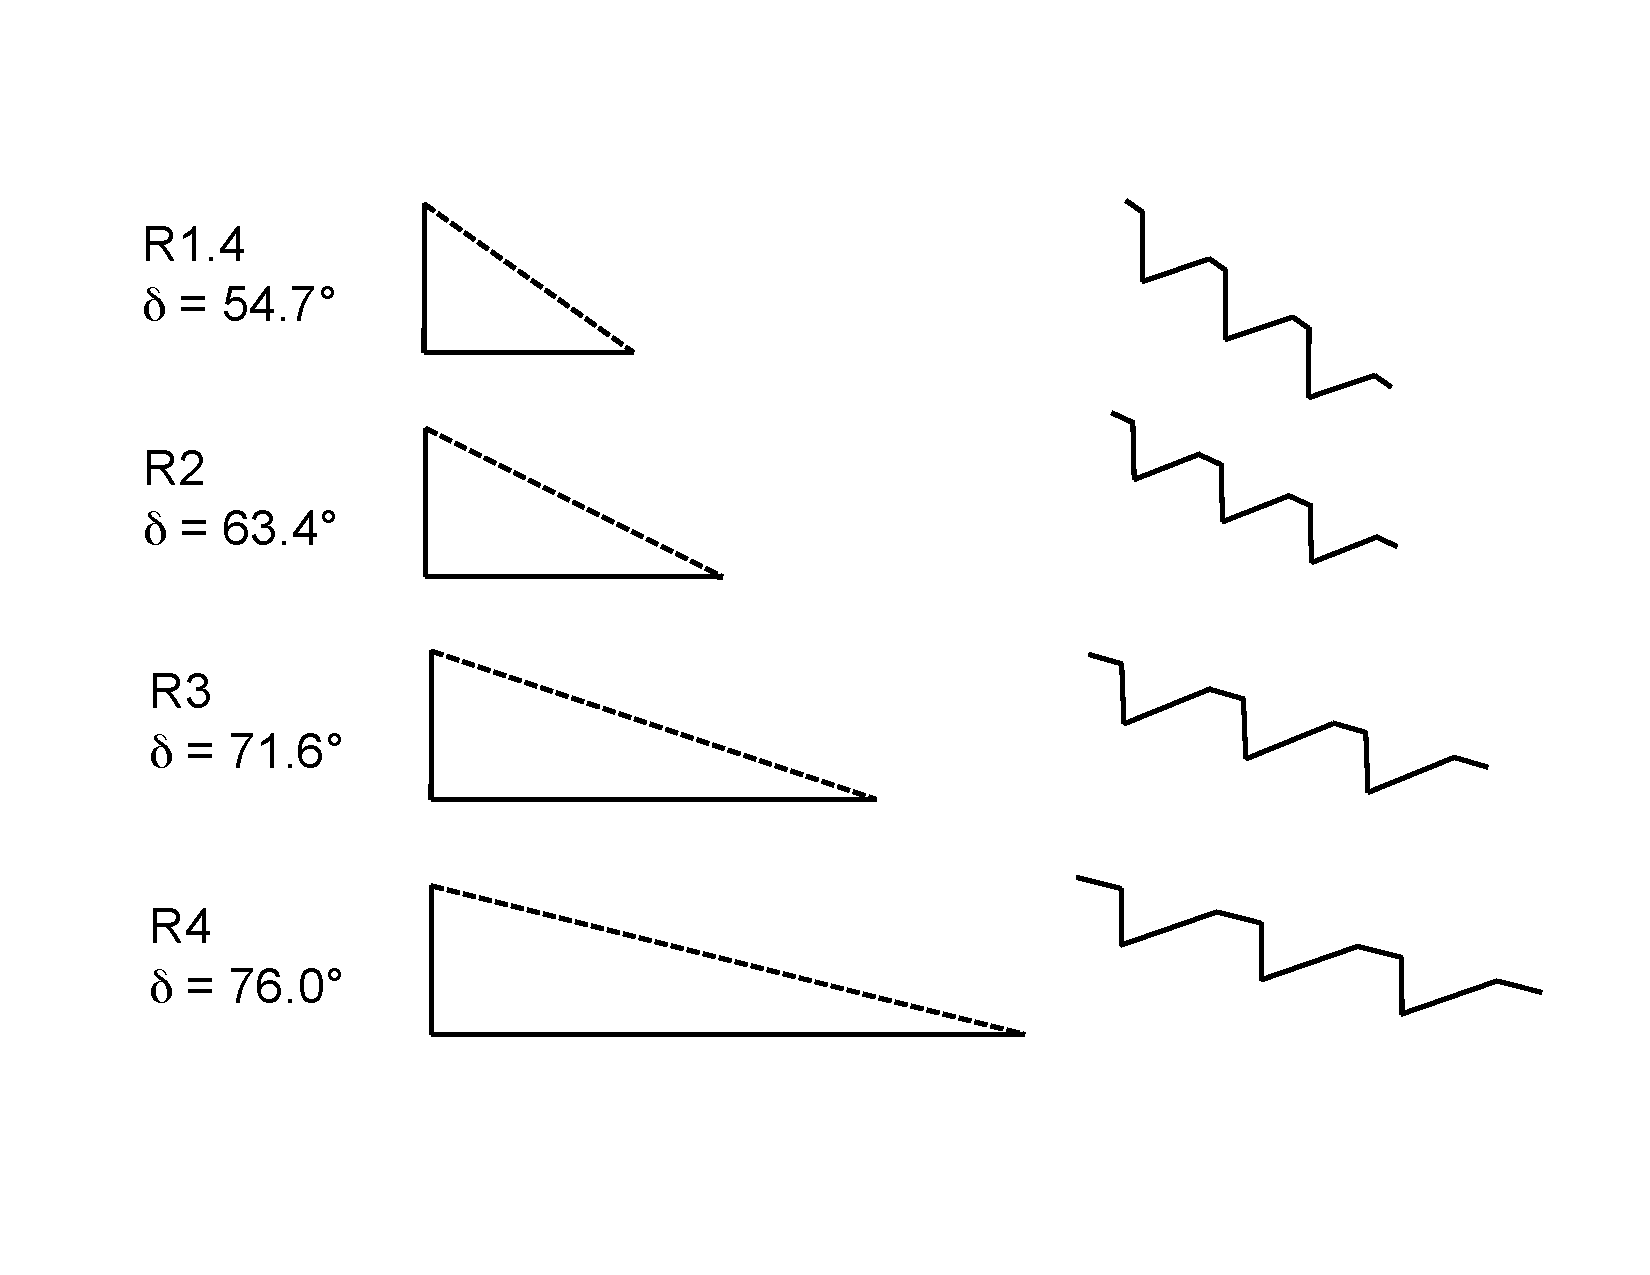
\psfig{file=chGratingDesign/Rnum,height=4.25in,width=5.5in}
\caption[Illustration of Si gratings of different blaze angles]{Illustration of Si gratings of different blaze angles, and the concomitant microscopic Si V-groove cross section.  The grooves are symmetric for R1.4, and increasingly asymmetric for larger blaze angles.  The apex angle of the cross section is 70.5$\deg$ in all cases; it is set by the Si crystal structure and is minutely increased by the finite anisotropic etch ratio.}
\label{fig:Rnum}
\end{center}
\end{figure}


\section{Groove top fill factor and geometric shadowing}
The groove top size has an allowable range.  The small size limit on the groove top is set by KOH under-etching, specifically the tops must be wide enough to hold up against the finite amount of under-etching.  Under-etching limits the groove top to a few percent of the groove width.  The large size limit for the groove top is set by geometric shadowing of the groove facets in a delivered device.  The geometric shadowing is illustrated schematically in Figure \ref{fig:groovetop}.  We derived the geometrical maximum groove top width above which the efficiency is degraded, described below.  We assumed for our derivation that light is incident normal to the groove facets, i.e. the Littrow configuration, which is a good assumption in immersion because of Snell's law.  The maximum allowable ratio of $t/\sigma$ is:

\begin{equation*}
t/\sigma < \frac{1}{1 + \frac{\tan(a)}{\tan(\delta)}}
\end{equation*}
Where $a$ is the Si Apex angle, and $\delta$ is the blaze angle.  For an R3 echelle we must have $t/\sigma < 0.51$.  For the LM module of iShell we elected to use a groove top $t=30 \; \mu$m, which is $t/\sigma=0.375$, so the groove tops will be safely shadowed in this device.  It makes sense that higher R-number gratings can tolerate larger groove tops, as can be surmised from the schematic Figure \ref{fig:groovetop} and the top pane of Figure \ref{fig:IGdesignplot}.


\begin{figure}[h!] 
\begin{center}
\ 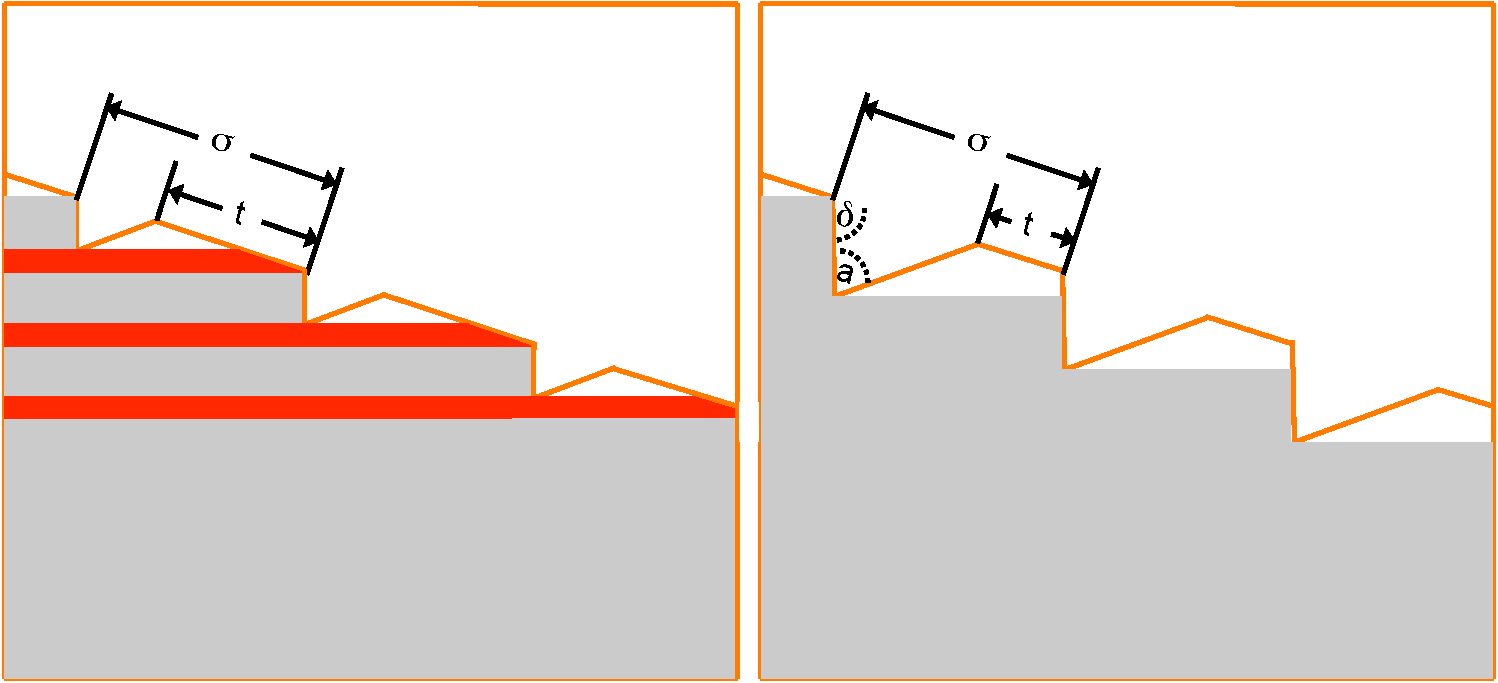
\psfig{file=chGratingDesign/gt_geom_blockage.pdf,height=3in,width=6.4in}
\caption[Schematic of groove top geometry]{Schematic of groove top geometry.  The cartoon gratings have the same blaze angle and period, but different groove top widths (fill factors).  There is a critical groove top width to period ratio below which the groove tops are completely shadowed and no geometric blockage occurs.  For an R3 grating as used in iSHELL, the critical fraction is $t/\sigma < 0.51$.  The delivered devices have $t/\sigma = 0.375$, which is similar to the schematic on the right side.}
\label{fig:groovetop}
\end{center}
\end{figure}

\begin{figure}[h!] 
\begin{center}
\ 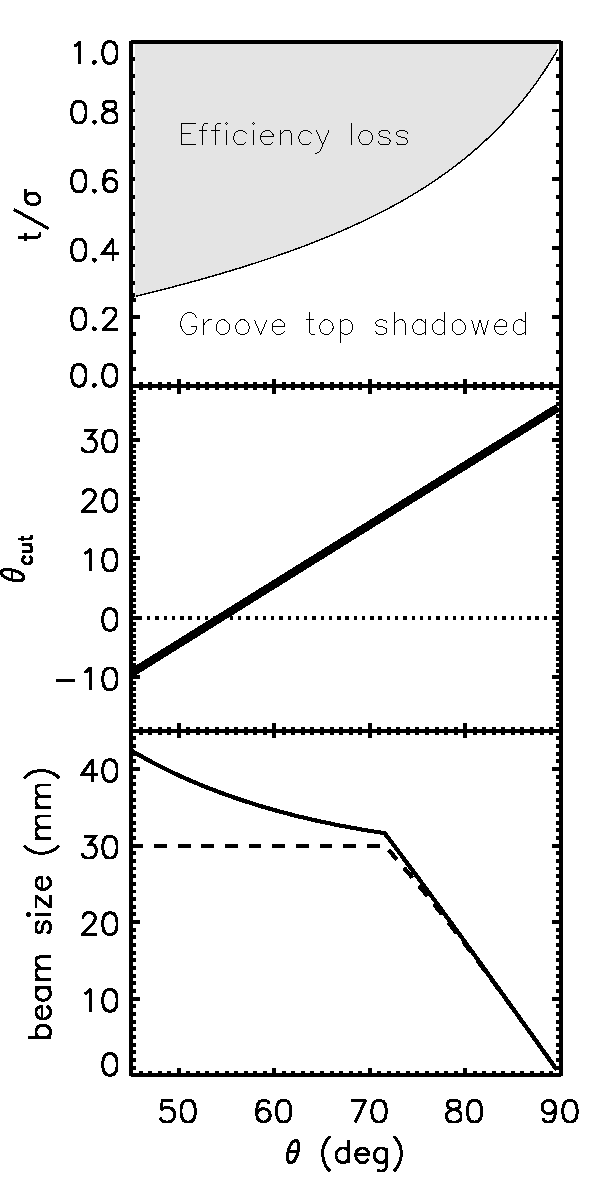
\psfig{file=chGratingDesign/IG_blaze_design.pdf,height=6.5in,width=3.25in}
\caption[Grating design considerations that depend on the choice of blaze angle]{Three paneled plot showing three grating design considerations that depend on the choice of blaze angle.  The top pane shows the range of groove top to grating period ratios that result in shadowed groove tops, or efficiency loss from exposed groove tops.  The middle pane shows the angle at which a Si boule must be cut to produce Si V groove facets at the given blaze angle.  The thickness of the line in the middle pane is equal to the range in cutting angle depending on the degree of anisotropic etching into the (111) Si crystal plane (and concomitant widening of the Si V-groove apex angle).  The width corresponds to $<0.8\deg$.  The bottom pane shows the maximum beam size possible on a 30 mm thick, 100 mm diameter Si substrate, as a function of blaze angle.  The solid line is the beam size, the dashed line is the substrate thickness as measured perpendicular to the grating surface.  These figures are all for Si immersion gratings in Littrow autocollimation.}
\label{fig:IGdesignplot}
\end{center}
\end{figure}

\subsection{Scarp face size in optical reflection measurements}
The proposed GMTNIRS grating LM module will require a larger beam size and a larger illuminated length than the IGRINS or iSHELL immersion gratings.  The strawman design requires an 8 inch substrate, which seems daunting given the challenges of immersion grating production on smaller 4 inch substrates.  Alternative designs employing an R4.5, rather than R3, grating are being considered.  High-R gratings have the limitation that the scarp facet length shrinks for larger blaze angles, until some threshold at which the scarp face is obscured.  The most important diagnostics for evaluating the performance of prototype immersion gratings require the scarp face to be visible.  

\begin{figure}[h!] 
\begin{center}
\ 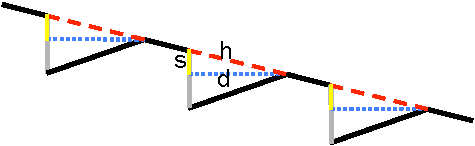
\psfig{file=chGratingDesign/scarp_reflect.pdf,height=2.0in,width=6.3in}
\caption[Scarp facet in reflection]{A diagram illustrating the lengths used to define the scarp face geometry when illuminated in back surface reflection.  The scarp face length $s$ is labelled and shown in the vertical short solid yellow line.  The blaze angle is the enclosed angle of line $s$ and $h$.  The hypotenuse of the right triangle is label $h$ in the long dashed red line.  The short blue dashed line is perpendicular to the scarp face and parallel to the incoming beam.  }
\label{fig:scarpface}
\end{center}
\end{figure}

Equipped with the geometrical definitions of \ref{fig:scarpface} we can determine $s$:
 \begin{eqnarray}
h=\sigma-t \nonumber \\
\cos{\delta}=s/h \nonumber \\
s=(\sigma-t)\cos{\delta}
 \end{eqnarray}

For an R4.5 grating, $\delta=77.5^\circ$, so the scarp facet $s$ is 20\% of the length $h=\sigma-t$.  There is no angle for which the scarp facet is completely shadowed, although it is true $s$ shrinks for large blaze angles.  Optical tests performed in reflection on higher blaze gratings will have a smaller scarp facet to probe, and the concomitant broad blaze envelope associated with convolving orders with the transform of narrow slit functions.  




%
\chapter{Immersion grating process and production}

\section{Heritage}

%\citep{2007ApOpt..46.3400M}
The work I have done on gratings during my 5 year career in the Si diffractive optics group has built upon the decades long effort of the previous generation of researchers.  In this section I briefly summarize the heritage upon which this dissertation has grown.  The most recent refereed publication on the production of our gratings is Marsh, Mar, and Jaffe's 2007 Applied Optics paper titled ``Production and evaluation of silicon immersion gratings for astronomy'' .  The Applied Optics paper came out of Jasmina Marsh's Ph.D. dissertation work, which was almost exclusively on the topic of gratings and grisms.  Jasmina contributed immensely to the current state of production and metrology of gratings.  Katelyn Allers worked simultaneously with Jasmina.  Katelyn's contributions included expanding the grating production to the Pickle Research Campus (PRC) Microelectronics Research Center (most often abbreviated MER, but sometimes also MERC or MRC).  Katelyn characterized the pattern transfer process, specifically in the plasma etch step that we will describe in detail in a later section of this chapter.  Before both Jasmina and Katelyn, Luke Keller was one of the first graduate students who pioneered a lot of the diffraction grating production on wafers.  The institutional memory before Luke has not survived as well.  I overlapped with Jasmina Marsh for about a semester or so.  Casey Deen overlapped with both Jasmina, Katelyn, and me.  Casey was a jack-of-all trades, of sort.  He shepherded the UV exposure system from its old formation to its current form, a metamorphosis described in detail in a later section of this chapter.  Casey also made the initial prototype of our grating efficiency tester, the so-called Custom Robotic Order, Wavelength, and Blaze-Angle Recorder (CROWBAR).  Concurrently with Casey and me, Hyeonju Jeong  was a visiting graduate student for over a year.  

\section{Spin coating}
We use Microposit S1800 series positive photoresist from Microchem.  The S1800 series was historically produced by Shipley, a Boston-area based company, which now appears to be out of business.  The S1800 product is still available through Microchem, which is a distributor for Dow Electronic Materials.  The Microchem website is \url{http://microchem.com/}.  There is not much other information available on the web for this series of resists.  The six-page product guide for the S1800 resists available on the Microchem site is reproduced in its entirety in the appendix for convenience.  There are at least five varieties of the S1800 resists all prefixed with S: 1822, 1818, 1813, 1811, 1805 in order from highest to lowest viscosity.  The resists differ primarily in their viscosity, and therefore the delivered resist thickness for a given spin speed and spin duration.  We do not dilute our resists.

The large size, asymmetric shape, and large thermal mass of our 30 mm thick Si pucks make spinning and baking a challenge.  The spin speed is typically between $\omega=1800-2200$ RPM for 60-90 seconds.  We arrived at these speeds and times by weighing the safety and performance tradeoffs of high angular speeds.  The safety concerns are based on the understanding that a fast rotating mass contains a considerable amount of kinetic energy, which could conceivably be transferred into translational kinetic energy to act as a dangerous projectile.  Specifically we calculate the approximate energy $E$ of a projectile possessing mass $m=550$ g and angular velocity $\omega=2000$ RPM for a solid cylinder with radius $r=50$ mm and height 30 mm.

\begin{eqnarray}
       E&=&\frac{1}{2}I \omega^2 \nonumber \\
		&\sim&15 \textrm{ Joules} \nonumber
\end{eqnarray}

The total kinetic energy of 15 Joules is comparable to a 30 MPH fastball, which is not too bad, but not pleasant either.  Since the energy goes as the square of the angular velocity, a spin speed of 6000 RPM would be 9 times more energy, or a 90 MPH fastball.  We see no performance limitations spinning at 2000 RPM, although we have not experimented on thick substrates at higher spin rates due to safety considerations.  The spin curve for S1805 is included in the Shipley technical document included in the Appendix Section \ref{sec:A1s1800}.  The spin curve for S1805 in that document's Figure 1 shows a film thickness equal to about 600 nm for 2000 RPM spin speed.  Our direct measurements with ellipsometry and stylus profilometry indicate film thicknesses around 600 nm with a 15\% thickness range.  The observed thickness range is consistent with our range of spin speeds and the plot in the Appendix \ref{sec:A1s1800}.

Surface tension effects cause thick buildup of resist, called the edge bead, at the outer few millimeters of the substrate.  The edge bead prevents close contact between the photoresist film and the chrome mask.  Our strategy for edge bead removal is to drag a miniature acetone soaked swab over the outer 2-3 mm.  We explored the performance impact of edge bead removal by comparing two identically prepared wafers with and without edge bead removal.  The wafer that had undergone edge bead removal was uniform upon visual inspection.  The wafer with no edge bead removal demonstrated broken lines over about one third of the wafer surface.  Tests without edge bead removal have resulted in uniformly developed patterns, so edge bead removal probably offers modest advantages some of the time.  Its effect on thick pieces has not been studied in detail, but anecdotally the best piece ever produced in terms of large scale surface flatness, CA1, had edge bead removal performed before contact lithography.  We have no reason to believe that edge bead removal will affect electron beam lithography.  

Figure \ref{fig:spincurve} shows the angular speed as a function of time during spinning.  The recipe pictured has a peak angular speed of 2100 RPM, resulting in a resist thickness of $802 \pm 6 $ nm.  

\begin{figure}[h!] 
\begin{center}
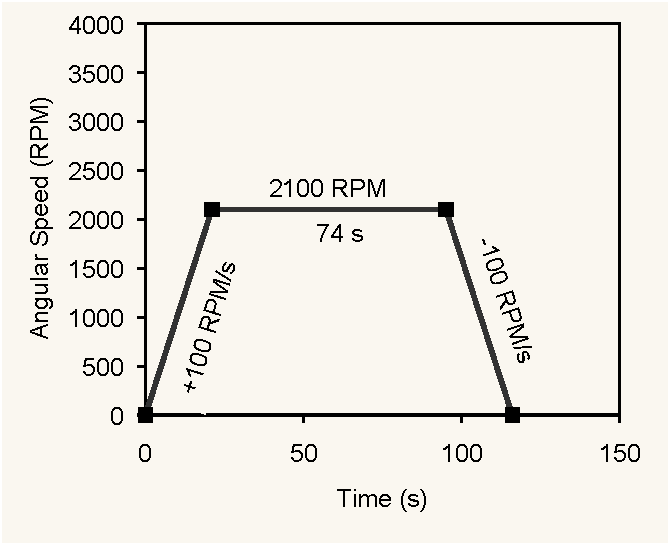
\psfig{file=spincurve,height=2.75in,width=3.25in}
\caption[Photoresist spin curve]{Spin curve for spinning photoresist on massive substrates.  The ramp angular acceleration is 100 RPM/s for 21 seconds, followed by constant angular speed of 2100 RPM for 74 seconds.  The deceleration is 100 RPM/s.}
\label{fig:spincurve}
\end{center}
\end{figure}

\section{Issues related to the photoresist}
Appendix \ref{sec:A1s1800} contains 4 pages from a vendor-provided technical document describing the properties of S1800 series photoresists from Shipley.  Dow chemicals now produces this photoresist under its subsidiary Microchem.  The general behavior of this photoresist should be similar to any positive photoresist, but with slightly different refractive index, resist thickness spin curves, contrast, etc.  In this section we analyze the plots provided in the Shipley technical document to better understand the effect on our UV contact lithography.  The Shipley document largely describes the S1813 photoresist, whereas we use S1805 photoresist.  I am led to believe that these differ only in their dilution, so that they should be identical in all their post-spin bake properties.

\subsection{How to treat ellipsometrically derived thin film thickness}
In this section I rely heavily on measurements of thin film thickness carried out with ellipsometry.  Ellipsometry works by measuring the angular and wavelength dependent elliptical polarization of a small patch (a few mm diameter) of a thin film.  The expected elliptical polarization can be modeled and fitted to the observed data to yield a best fit thickness, or other physical properties that affect the polarization at an interface.  A key aspect of ellipsometry is that you must provide the wavelength-dependent refractive index to accurately fit for the film thickness.  We Cauchy coefficients (XX) provided in Figure 3 of \ref{sec:A1s1800}.  We fit the ellipsometry data in the wavelength range $\lambda = $ 600$-$1000 nm.  We do not fit shortward of 600 nm despite the availability of data to 200 nm.  The reason is that the resist layer is absorptive shortward of 500 nm.  In the range 500 nm to 600 nm, the model fits were poor, suggesting that the refractive index model is especially poor in this wavelength range, which makes sense since the refractive index is a steep function of wavelength in this region.

Our tool is the Woollam M-2000 series ellipsometer.  We have access to two mostly identical versions of this tool, one at the Center for Nano Mechanics (CNM) cleanroom at the UT Austin main campus and another at the Pickle Research Center's Microelectronics Research Center (MRC).  Both tools are in clean environments and function identically.  The CNM tool has a fine adjust translation stage with 2'' range of motion and 0.001'' tick marks on the micrometer scale in both the $x-$ and $y-$ axes.  The MRC tool has no fine adjust translation stage.  We typically sample at intervals of 5\degree angles of incidence in the range 41-76 \degree as measured from the normal to the film surface.

I quantified the impact of changing the refractive index profile to estimate the uncertainties in the film thickness derived with ellipsometry.  Specifically, we computed the thickness derived from the Shipley-provided Cauchy coefficients and the thickness derived from a simultaneous fit to the thickness and refractive index optical constants.  The difference between the two thicknesses derived in this way is typically minuscule (0.3\%), but can be as high as 10\% if the elliptical polarization model fit is poor.  We assigned this uncertainty to the thickness, rather than the much smaller uncertainty reported in the software.  

It is conceivable that there is a systematic error in using ellipsometrically derived film thickness measurements.  We assume that the systematic errors are captured in the uncertainty we assign, and otherwise are negligible.  The biggest concern is the uncertain wavelength-dependent refractive index, which we account for in reporting our uncertainties.  A second less likely problem is that our knowledge of the underlying silicon nitride thickness is uncertain at a 10\% level.  I am led to believe that the thickness of the second layer has negligible impact on the ellipsometric model, and instead it is mostly the interface of the material with the top most thin film that plays a dominant role.  Lastly, we have assumed ideal properties when deriving models of our ellipsometry.  We know that in some cases the resist is non-uniform over the few millimeter beam size, which will smear out polarization signals, but these effects are likely to be miniscule.

\subsection{Do initial variations in the photoresist thickness degrade the grating performance?}
In this subsection I answer the question ``to what extent do initial variations in the photoresist thickness contribute to performance degradation?''.  Anecdotally, the resist coating process must be fairly uniform since spin-coated wafers have the same color photoresist everywhere- if there were dramatic thickness variations we would see different colors, like when there is a comet that messes up the photoresist.  To check our intuition, I directly measured the photoresist thickness in 5 different points on a spin-coated but unexposed wafer.  I measured the resist thickness with the Woollam M-2000 series ellipsometer at CNM.  The wafer was prepared with our usual recipe with the spin curve shown in Figure \ref{fig:spincurve}.  The thickness in the center was 806.9 $\pm$ 2.6 nm, while at a location 2.8'' away the thickness dropped to 799.7 $\pm$ 1.8 nm.  The uncertainties in the difference of resist thickness are much less than the systematic error reported, so the trend and level of the difference is firm.  The peak to valley variation of our 5 data points is 0.9\%.  The resist is remarkably uniform.  Still, the phenomena of interference and high contrast in photoresists means that we have to convert the level of this initial thickness variation into an exposure time difference in order to rule out initial film thickness as a source of performance degradation in immersion gratings.

Figure 4 in \ref{sec:A1s1800} shows a plot of interference curves ($E_0$ vs thickness, where $E_0$ is the critical dose) for our resist in the thickness range 1100-1400 nm.  Our $\sim$800 nm resist thickness is well outside this range.  I performed a by-eye fit to the data including a sine wave with a linear and constant term: $E_0=A\sin(2\pi [t-t_0]/T) + Bt+C$.  I extrapolated this fit past 800 nm.  Figure XX shows the digitized data points from Figure 4 in \ref{sec:A1s1800} in red, my fit to those data points in blue, and the extrapolation in yellow.  This strategy is highly uncertain- I do not even know if my model of a sinusoidal variation is accurate.  With that proviso, the fit looks fairly convincing, and 800 nm is right on the part of the interference curve with the maximum slope.  This means our choice of resist thickness (more specifically, our choice of maximum spin speed), is unfortunate.  The minute variations in initial resist thickness are amplified in the requisite dose to clear.  One glaring problem with my model is the direction of the variation is all wrong- the observed resist is thicker in the middle than the edge, whereas my model predicts that the center should have a lower critical dose and therefore be thinner than the edge.  There are a few places why this model failed.  First, my projection is probably not accurate.  Second, the data is for the case of G-line only UV illumination, whereas the spectrum of our UV lamp (c.f. Figure XX) has a broad spectrum of other bright lines which will wash out the sharp peaks of Figure \ref{fig:S1800interference}.   

\begin{figure}
\begin{center}

\subfloat[Projected photoresist interference curve]{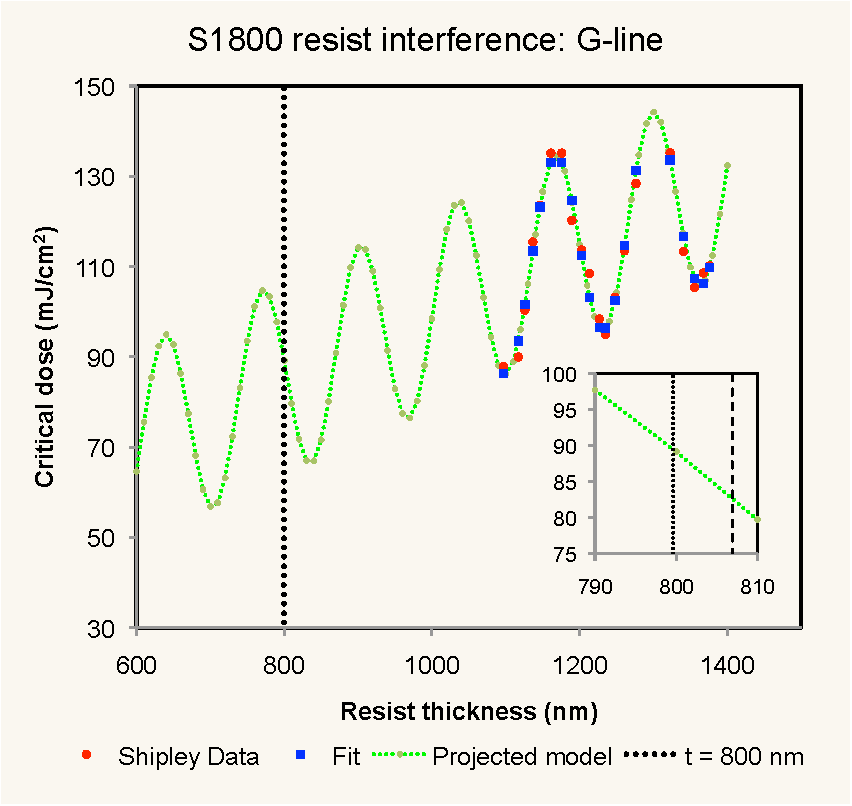
\psfig{file=chGratingProcess/S1800interference.pdf,height=2.75in,width=3.25in}}
\\
\subfloat[Center to edge variation assuming the projected interference]{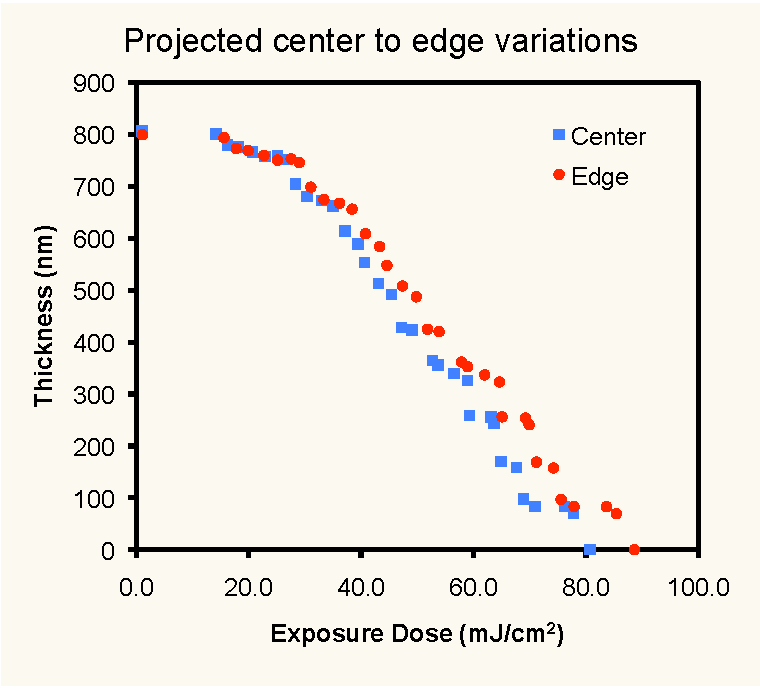
\psfig{file=chGratingProcess/projectedC2Evariation.pdf,height=2.75in,width=3.25in}}
\caption[Projected photoresist interference]{The projected photoresist interference assuming mercury G-line wavelength exposure.  The inset shows a blow-up of the thickness range surrounding the thickness of our photoresist, 800 nm.  The thickness of our resist ranges from 807 nm at center to 800 nm at edge, which corresponds to a projected critical exposure difference of 82 mJ/cm$^2$ to 90 mJ/cm$^2$.}
\label{fig:S1800interference}
\end{center}
\end{figure}

The second panel of Figure \ref{fig:S1800interference} shows the estimated thickness as a function of dose for the case of the center thickness 807 nm and edge thickness 800 nm, with the projected interference from the first panel of the same figure.  The 0.1\% difference in resist thickness can translate into a 60-80 nm difference for otherwise identical exposure time.  With my assumptions of the interference curve, the locations where the resist is initially thinner will actually stay thicker longer, owing to their larger critical dose to clear.  This result is a little bit shocking, but remember this is an upper limit on the effect, assuming maximum slope on the interference curve.  It is worth investigating to what extent our resist is monochromatic or broadband.  In the next section we seek to answer this question.

\section{Which wavelength range is most effective in illuminating the resist?}
The delivered dose depends on the spectral characteristics of the UV light source and the absorption properties of the resist.  I computed the product of these curves to construct the absorbed power as a function of wavelength.  I digitized the S1800 absorption as a function of wavelength curve in Figure 6 of the Shipley technical document in \ref{sec:A1s1800}, only for the unexposed resist curve.  I smoothly extrapolated the absorption past 500 nm, assuming 0.1\%absorption for $\lambda > 535$ nm.  I similarly digitized the vendor-provided UV spectrum of the Omnicure 2000 lamp, which I accessed from the Omnicure website.  I interpolated both curves onto a wavelength scale from 250$-$700 nm at 2.5 nm intervals, then took the product of the curves.  The result is shown in Figure \ref{fig:UVabsSPEC}.  It appears that all three strong UV mercury lines (I-, H-, and G- lines; 365, 405, 436 nm) contribute to the exposure of the resist.  The polychromatic exposure questions the assumption of using the curves provided in the Shipley technical guide, since the guide explains that the illumination source is G-line only.  In our plot, the G-line accounts for a small fraction of the power.  

\begin{figure}[h!] 
\begin{center}
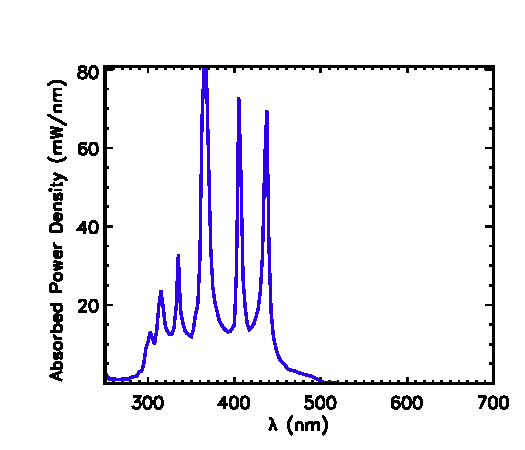
\psfig{file=chGratingProcess/UV_spec_abs.pdf,height=3.0in,width=3.50in}
\caption[UV absorption and lamp spectrum]{The absorbed power density as a function of wavelength.  This curve is the product of the lamp wavelength and the absorption of the S1800 photoresist.  See the text for the assumptions and extrapolations.  The line at 435 nm is the mercury G-line.  It is clear that the other lines contribute strongly to the delivered dose of the S1800 photoresist.  These other peaks should smear out the interference curves shown Figure \ref{fig:S1800interference}.}
\label{fig:UVabsSPEC}
\end{center}
\end{figure}



\section{UV mask contact lithography}
Figure \ref{fig:uvsys} shows a schematic of our UV contact photolithography system.  The UV light source is an Omnicure S2000.  The Omnicure spectral properties have not been independently verified, but are shown in Figure \ref{fig:UVabsSPEC} as the product of the unexposed absorption of the photoresist and the lamp output.  The S1805 photoresist is optimized for mercury G-line (435.8 nm), but it is effective with broadband exposure.  The major property of photoresists is their critical polymerization upon exposure to UV light.  In the positive photoresists like the S1805 we use, the area exposed to UV light is polymerized, and develops away.  The area shadowed by chrome masking remains.  Figure 7 in Appendix \ref{sec:A1s1800} shows how the normalized photoresist thickness remaining depends on the delivered dose.  One major property we care about is the so called ``dose to clear'' or ``critical dose'', denoted as $E_0$ in Figure 7 in Appendix \ref{sec:A1s1800}.  The critical dose is an intensity above which the photoresist is polymerized and below which there is no change in the photoresist properties.  An ideal binary resist will have an infinitely sharp transition- a step function- from cleared to uncleared.  Real-world resists have a finite and gradual transition from uncleared to cleared.  Specifically, the post-development resist thickness will monotonically decrease as a function of exposure until it reaches the critical dose, and then no further reactions will take place.  The chemistry of how this reaction takes place is beyond the scope of this report, and is summarized elsewhere (cite XX).  Suffice it to say, photoresists of all varieties have been created to have a variety of properties.  


\begin{figure}[h!] 
\begin{center}
\ 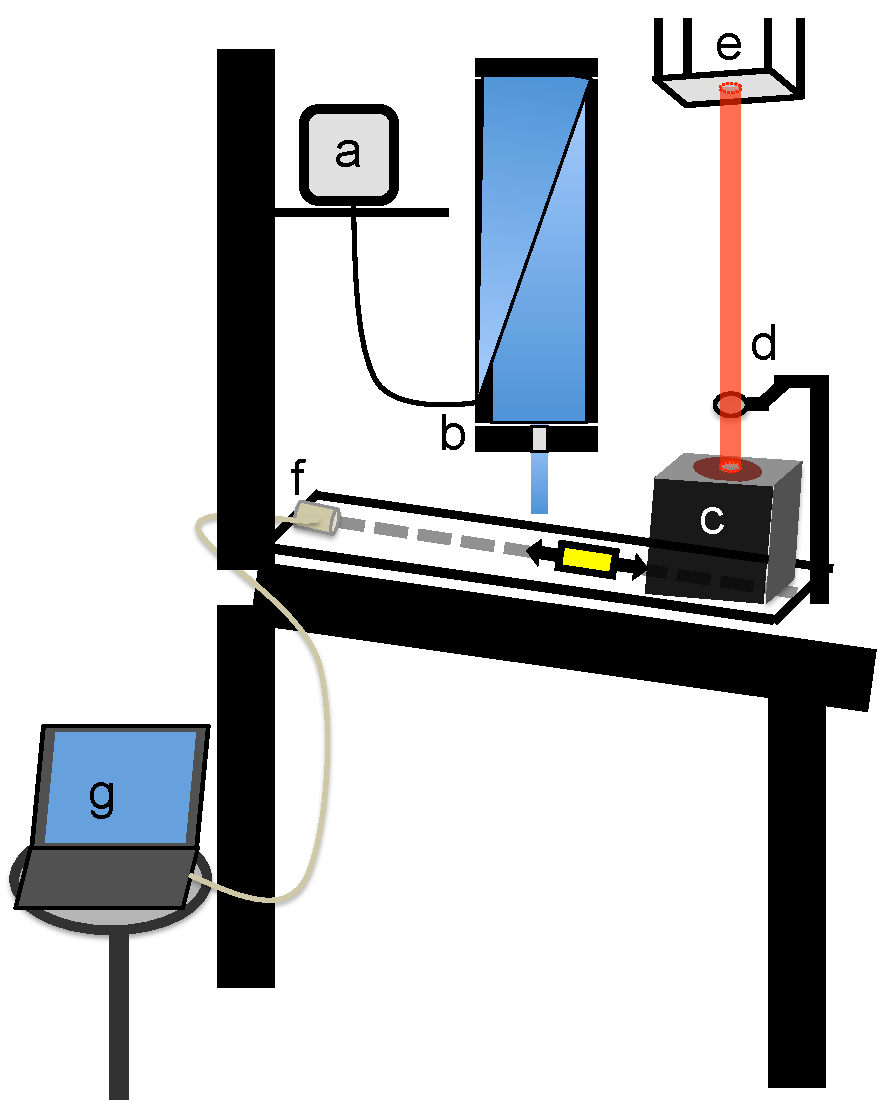
\psfig{file=chGratingProcess/UV_expos_graphic2.pdf,height=4.5in,width=4in}
\caption[Schematic of our UV exposure system]{Schematic of our UV exposure system.  The UV exposure system operates by moving the mask-substrate unit beneath a stationary UV light source.  The key components of the system are labeled.  The ultra stable UV lamp (a) is fiber fed to a collimating mirror, before passing through a 1'' $\times$ 6'' slit (b) with its long axis perpendicular to the direction of motion of the car (c).  A 632 nm laser beam (d) illuminates a 1'' diameter beam on the mask-substrate unit to aid in minimizing Newton's rings fringes from poor contact.  The beam is viewed on a white card (e).  A computer controlled motor (f,g) controls the delivered exposure dose by defining the rate of motion and number of passes for the car.}
\label{fig:uvsys}
\end{center}
\end{figure}

\begin{figure}[h!] 
\begin{center}
\ 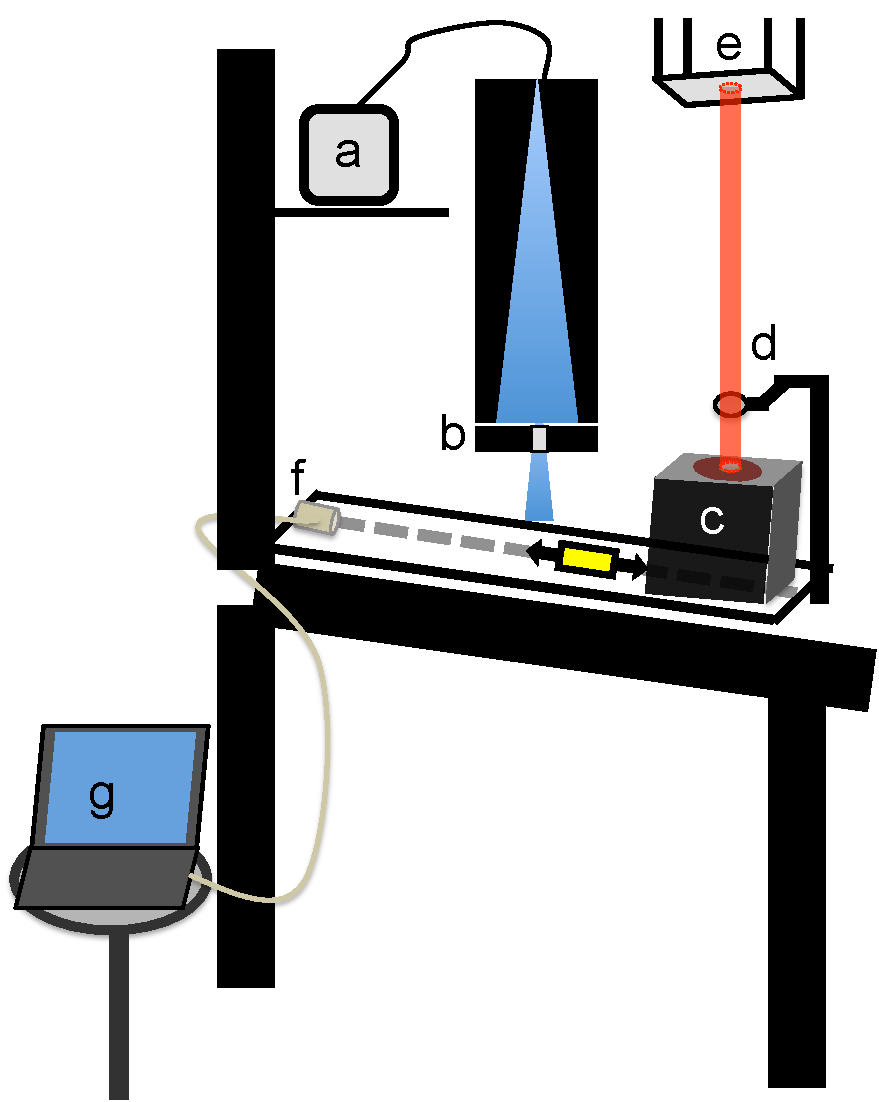
\psfig{file=chGratingProcess/UV_expos_graphic1.pdf,height=4.5in,width=4in}
\caption[Schematic of our former UV exposure system]{Schematic of our setup for the UV exposure system before 2010.  The key difference of the previous exposure system and the current system is the strategy for illumination, specifically collimation.  In the old system we simply had the light guide directed downward from the top of the tower, whereas in the new system we have a mirror at the top of the tower to receive the divergent beam from the light guide and subsequently collimate the beam toward the slit.}
\label{fig:uvsys}
\end{center}
\end{figure}

Our main concern with photoresist has to deal with where exactly the position of the critical dose is met in the vicinity of the chrome line edge position.  There are a variety of factors that contribute to the critical dose position.  Figure \ref{fig:dose2clear} shows the normalized thickness of resist as a function of exposure dose.  We constructed this photoresist contrast curve by exposing a resist coated wafer without a lithographic mask.  We masked 14 subregions of the wafer with a red film, exposures ranging from 36 to 0 passes.  Figure XX shows a photo of the wafer demonstrating the apparent non-uniformities.

\begin{figure}[h!] 
\begin{center}
\ 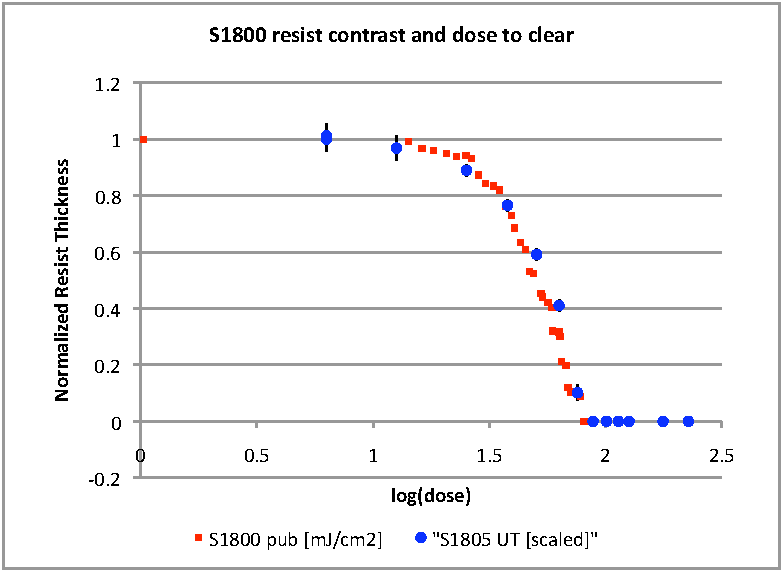
\psfig{file=chGratingProcess/dose2clear.pdf,height=4in,width=5.5in}
\caption[S1800 photoresist contrast curve]{S1800 photoresist contrast curve.  The red points are digitized values from Figure 7 of the Shipley S1800 series photoresist guide.  The $x-$ axis is the log of the exposure dose in mJ/cm$^2$.  The blue points are UT lab-measured values in number of passes plus a constant $x$ offset to match up with the scale on the Shipley measured values.  We know from the Shipley report that their values are for S1813 resist thickness 1230 nm, whereas our S1805 resist thickness is 700 nm, so we do not expect the dose to clear to be equal for these two different cases.  In fact, Figure 4 in the Shipley product guide shows that the dose to clear, $E_0$, can vary by 50\% for an 8\% change in resist thickness.}
\label{fig:dose2clear}
\end{center}
\end{figure}


\begin{figure}[h!] 
\begin{center}
\ 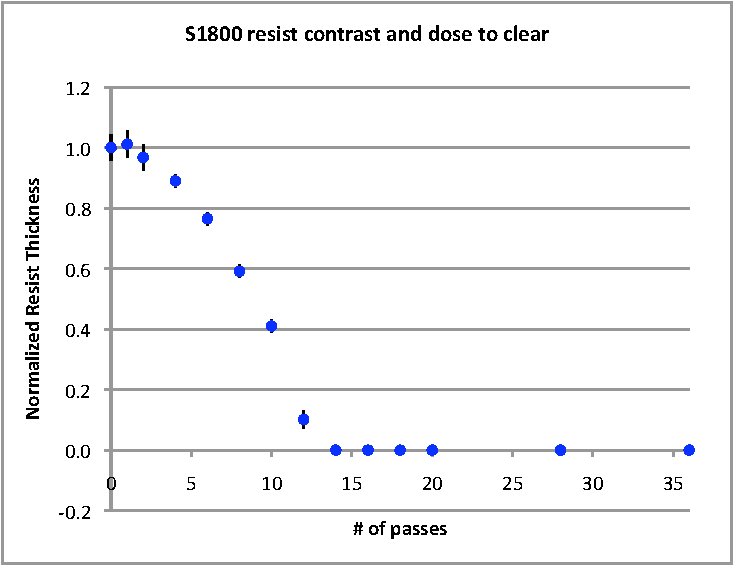
\psfig{file=chGratingProcess/dose2clear2.pdf,height=4in,width=5.5in}
\caption[Experimental photoresist contrast curve]{Photoresist contrast curve in units of number of passes on a linear scale.}
\label{fig:dose2clear2}
\end{center}
\end{figure}


\begin{figure}[h!] 
\begin{center}
\ \psfig{file=chGratingProcess/IMG_3285.jpg,height=5in,width=4in}
\caption[Photo of experimental wafer]{Photo of the wafer used to make figures \ref{fig:dose2clear2} and \ref{fig:dose2clear}.  The large scale non-uniformities are apparent at the region near the critical dose.}
\label{fig:dose2clearphoto}
\end{center}
\end{figure}

\begin{figure}[h!] 
\begin{center}
\ \psfig{file=chGratingProcess/3Dzoomw20120926.pdf,height=5in,width=6.25in}
\caption[Zygo interferometry of experimental wafer]{Zygo interferometry at maximum zoom.  The target is the wafer shown in the photo in Figure \ref{fig:dose2clearphoto}, centered around the region near the critical dose.  The 3D map shows fine spatial structure that is barely perceptible.  The steps are approximately 5 mm wide.  }
\label{fig:3dZYGOresist}
\end{center}
\end{figure}

The UV exposure step is probably the most critical and most mysterious step in our device production process.  In the subsection below I will enumerate some of the dominant unknowns in the UV exposure step.  Part of the reason why there is some mystery in the system is because experiments are costly in hardware and effort.  Consumable and costly thick Si pucks are required to probe the quality of contact, since wafers are too flexible.  Experiments with thick pieces are often inconclusive anyways, given the large amount of uncontrolled variation in other parts of our process and the small number of experiments, owing to the per-part cost.  Consider the following example.  In the summer of 2011 Dr. Weisong Wang and I were seeking to make the iSHELL LM immersion grating on the recently overhauled exposure system.  The overhaul had improved the UV beam collimation but the system suffered an 80\% light loss as a result.  Our first experiment E\#\# (XX)  yielded a peak to valley surface error of about 0.8 waves over a 25 mm beam at R3.  Weisong and I proposed that the exposure dose was insufficient, and we were merely operating in the exposure regime near the critical dose where minute changes in the dose are amplified into large position deviations of line edges.  Our solution was to try exposing another part with a longer exposure time.  So we made part (E\#\# XX), which demonstrated identical performance to the previous (poor) E\#\# (XX).  There was no change in performance.  What did we learn from this series of experiments?  The per-part cost of thick pieces is prohibitive, which we already knew, but appreciated more after a part was spent in vain.  We learned that it is better to design an experiment that will unambiguously answer which effect is dominant among our milliard steps.  For example, we did not necessarily find out that the exposure time was not to blame, given that we simply could have still been near the critical dose regime- that is, maybe we just did not increase our dose enough.  


There are many unknowns in the UV exposure step.  How good is the contact between the photolithographic mask and the Si substrate?  Does the contact change with time and temperature?  Specifically, does the movement of the car jostle the mask and substrate with respect to each other?  What is the degree of collimation of the UV beam?  What is the profile of the beam along the length of the slit, and more generally what is the 2D beam uniformity?  Does the profile of the beam along the length of the slit change in time?  Does the UV lamp intensity change in time?  To what extent is the beam non-uniform; how does the uniformity compare to vendors of mask aligners.  How does dose variation translate to a phase error?  Does the lamp have periodicity on short timescales ($\tau < 10 $ s) that will appear as periodic linewidth variations?  Similarly, does the lamp have long term drift so that the exposure time is lengthening or shortening in time?  Does firm contact between the mask and substrate peel off some of the photoresist, causing point defects?  Does resist from previous contacts stick to the mask and prevent good contact on future trials?  How good is the mask to begin with?  What is the UV sensitivity spectrum for the resist we are using?  What is the delivered intensity of our UV exposure system?  What is the dose?  What is the process latitude for our combination of developer concentration, dose, develop time?  Should we use a post-exposure bake?  Do we see standing waves in the vertical cross sections of our resist features?  Is there anything to gain by changing the spectral properties of the illumination, namely more or less bandwidth, or longer or shorter average wavelength?

\subsection{What is the beam intensity uniformity?}
The beam intensity spatial uniformity is important because the minuscule intensity variations implant phase errors in the resist sidewalls which translate into phase errors in our gratings.  Our dilemma is similar to taking a flat field during astronomical calibrations.  How uniform can a light beam be made?  The industry standard is the mask aligners of Karl Suss and others.  Suss specifies the UV illumination uniformity in their product datasheets available on their website \url{http://www.suss.com/en/products-solutions/products/mask-aligner/ma300-gen2/overview.html}.  For example, the MA300 Gen-2 has an intensity uniformity of 3-5\% depending on the wavelength chosen, but it is important to note that this uniformity is over the 12 inch diameter for their large wafers.  The uniformity over the inner 4 inches must be much better than 3\%, probably 1\% or better.  At the time of writing, our group does not have a good way to directly measure the UV-intensity uniformity.  

We have indirect detection of non-uniformity from the grayscale lithography of un-patterned wafers.  The method is described in detail in other sections in this chapter.  It is not safe to attribute the observed morphology entirely to the beam intensity nonuniformity, since the initial film thickness and the development process are likely to contribute to the non-uniformity as we will show in the next sections.  Still we can estimate the non-uniformity by positing that the lion's share of the morphology seen in grayscale tests is from the exposure process.  With this assumption, the range in resist film thickness is indicative of the range in UV exposure.  Figure 2.6 shows the vendor-provided dose-to-clear curve we have verified with our resist and substrate configurations.  Figure 2.7 shows the same measured curve on a linear scale.  Ellipsometry of grayscale exposed wafers shows that 80\% of the wafer surface has a resist film thickness in the range of 40 to 250 nm.  The initial film thickness is about 700 nm, so the normalized thickness variation is 5$-$35\%.  This magnitude of thickness variation corresponds to 18\% in UV dose non-uniformity.


\subsection{High spatial frequency structures in gratings}
High spatial frequencies in the context of our grating manufacturing are those structures that produce peaks in a monochromatic spectral impurities separated by a few diffraction widths, say $>5$ or so.  For a 25 mm beam, periodic structures with periods of 5 mm or less are considered high frequency.

One source of high frequency structures is the vibration of the turret and the car as the motor drives it forward.  Table xx summarizes the measured properties of the UV exposure system motion.  We measured the high frequency vibrations by resting an accelerometer on the fine adjust translation turret.  The STMicro STM33H 3-axis accelerometer was sensitive to frequencies of 0.1$-$40 Hz, with a target sample rate of 100 Hz, although we typically achieved only 90 Hz.  We sampled 2048 measurements over about 22 seconds.  We measured an RMS acceleration of 0.002 $g$ in the $x-$axis when the motor was at rest.  We tabulated the vibration frequency and amplitude for driving frequencies of 25, 43, 50, 67, and 200 rpm.  Figure XX shows the frequency and amplitude response of the motor for the range of driving frequencies.  

How does the vibration manifest in the exposure?  The linear position of a point on the wafer as a function of time is given by:

\begin{eqnarray}
 x(t)= x_0 + v_0 t + A \sin(2\pi f t - \phi)      \nonumber \\
 0 < x_0 < 100 \text{ mm}
\end{eqnarray}

Where the average speed $v_0$, amplitude $A$, and frequency $f$ comes from Table XX, and $\phi$ is arbitrary.  The UV slit width is 1".  The vibrating wafer slides under the UV slit, imprinting the phase difference of the entrance and egress from the light beam as a tiny exposure time difference that is periodic.  The period is about 210 $\mu$m, with an ans Figure XX shows a schematic of the processes, the position of a point on the wafer as a function of time, and the calculated effect for slit width equal to 25.35 mm.  

\begin{figure}[h!] 
\begin{center}
\subfloat[Schematic of the Wafer and UV slit motion]{\ \psfig{file=chGratingProcess/UV_slit.pdf,height=2in,width=3in}}
\\
\subfloat[Vibration effect on position and dwell time]{\ \psfig{file=chGratingProcess/UV_vibrations.pdf,height=3in,width=6in}}
\caption[Motor vibrations schematic]{The effect of vibrations is to produce periodic exposure dose as a function of position.  The period is about 210 $\mu$m, which is equal to the observed frequency.}
\label{fig:uvvibs}
\end{center}
\end{figure}

\begin{figure}[h!] 
\begin{center}
\ \psfig{file=chGratingProcess/zeiss_period.pdf,height=4.6in,width=6in}
\caption[High frequency structure in the photo resist]{High frequency structure in the photo resist color difference as probed by optical microscopy.  The Zeiss microscope at 5x shows a field of view a bit over 1.2 mm wide, showing subtle periodic waves in the resist thickness.  The period is in the range of 200-240 $\mu$m.  }
\label{fig:zeissfreq}
\end{center}
\end{figure}


\subsection{Uniformity along the slit}

\begin{tabular}{lccr}
\hline
Property & Symbol & Typical Value & Range \\
\hline
Motor angular rotation (rpm) & $\omega$ & 50 & 0$-$300 \\
Linear speed (mm/s) & $v$ & 4.2 & 0$-$25 \\
Translation screw pitch (tpi) & $\phi$ & 5 & $\cdots$ \\
%Motor resonant frequency (rpm) & $\omega_0$ & 60? & 43-67 \\
Vibration frequency (Hz) & $f_{vib}$ & 20 & 16-26 \\
RMS vibration amplitude (mm) & $<x>$ & 0.050 & 0.005-0.050 \\
Slit width (mm) & $w$ & 25 & 10$-$25 \\
Exposure time per pass (s) & $t$ & 6 & $>1$ \\
Dose to clear (passes) & $E_0$ & 14 & 14?$-$34? \\
Dose to clear (mJ/cm$^2$) & $E_0$ & 60? & 20?$-$100? \\

\hline
\end{tabular}

\begin{figure}[h!] 
\begin{center}
\ \psfig{file=chGratingProcess/resonantmotor.pdf,height=2.5in,width=3.5in}
\caption[Motor vibration amplitude]{RMS vibration amplitude as a function of driving frequency of the motor.}
\label{fig:resonantmotor}
\end{center}
\end{figure}

\begin{figure}[h!] 
\begin{center}
\ \psfig{file=chGratingProcess/freqresponse.pdf,height=2.5in,width=3.5in}
\caption[Motor vibration frequency]{Peak frequency of vibration as a function of driving frequency.  The power is almost entirely in the $x-$axis, which is the direction of motion of the car.}
\label{fig:freqresponse}
\end{center}
\end{figure}


\section{Anisotropic KOH etching}
Figure XX shows a schematic of the KOH etching process for the example of a biased wafer.
In principle, the KOH etching process should merely transfer the line edge positions from the Silicon Nitride hard mask into the silicon facets.  It is plausible that different etch rates over the surface will unevenly etch the surface, producing minute facet position differences.  One conceivable scenario is that the 30 mm thick Si puck has a different initial temperature from the surrounding bath.  The bath is typically either 40$\deg$ C or 68$\deg$ C.  The puck will warm from the edge to center, so that for the short duration of the temperature transition, the Si surface will experience increased etching at the edge.  Center-to-edge variations consistent with this type of over-etched edge pattern are conspicuous in interferometry of all our pieces (XX check the JPL piece).  The pattern is a focus aberration.  The amplitude of the focus aberration has a wide range among the dozen flat pieces with measured inter.  The clear strategy for mitigating the center-to-edge etch gradient is to equalize the part temperature and KOH solution temperature.

A similar center-to-edge etch gradient will occur if the etching rate is diffusion limited, and the circulation is better at the edge than at the center.  KOH etching in our process regime is generally temperature (XX) limited (cite XX -fundamentals of microelectronics), so the enhanced etch rate will be much smaller than the temperature gradient, but the diffusion gradient will last over the entirety of the etch process and not merely the beginning.


%\chapter{iSHELL Immersion Gratings}

The Immersion Grating Echelle Spectrograph is a high resolution near infrared spectrograph for the 3.5 m NASA Infrared Telescope Facility (IRTF) located at the summit of Mauna Kea, Hawaii.  The spectrograph has two modules with different immersion gratings serving as the high resolution dispersing optical elements.  The two modules have wavelength ranges 1.2-2.5 $\mu$m and 3.0-5.0 $\mu$m.  The short wavelength module will have a resolving power $R=80000$.  The long wavelength module will have a resolving power $R=67000$.  We are producing the immersion gratings at the University of Texas at Austin.

\section{Specifications}
The design and specifications of iSHELL have been described elsewhere (Rayner et al. in press).  The table below lists the basic properties of iSHELL and the specifications for the immersion grating.

\begin{tabular}{llr}
\hline
& \multicolumn{2}{c}{Module} \\
\cline{2-3}
	 & JHK & LM  \\
\hline
\multicolumn{3}{c}{Basic Properties} \\
\hline
$\lambda$ range ($\mu$m) & 1.15-2.5 & 3.0-5.0 \\
$\lambda/n$ ($\mu$m) & 0.34-0.73 & 0.88-1.5 \\
resolution, $R$ & 80k & 67k \\
slit width, $\phi$ ('') & \multicolumn{2}{c}{$\ge$0.375} \\
$\lambda/D$ ('') & 0.07-0.15 & 0.18-0.3 \\
$\phi \lambda/D$ & 5.3-2.5 & 2.0-1.25 \\
\hline
\multicolumn{3}{c}{Grating Properties} \\
\hline
pitch, $\sigma$ & 48.5 & 80 \\
top, $t$ & TBD & 30 \\
fill factor & TBD & 37.5\% \\
blaze, $\delta$ ($\;^\circ \;$) & \multicolumn{2}{c}{71.5} \\
Si apex, $a$ ($\deg$) & \multicolumn{2}{c}{70.53+$\Delta a$} \\
$\Delta a$, ($\deg$) & \multicolumn{2}{c}{0.8} \\
Method  & e-beam & UV mask \\
\hline
\end{tabular}

A key figure of merit is the quantity $\phi \lambda/D$, listed in the above table.  $\phi \lambda/D$ is the number of diffraction limited resolution elements that fit inside the seeing disk.  It is a measure of the performance demand on the immersion grating in the following way.  The total delivered spot is the convolution of the PSF from the seeing disk and the PSF from the immersion grating- ignoring all other optics.  If the seeing disk is much larger than the diffraction limit, then the diffraction grating need not be diffraction limited.  The ``coherence length'', that is the length over which the grating must be in phase, is equal to the grating length divided by the factor $\phi \lambda/D$.


\section{iShell grating fabrication}

\subsection{Substrate properties and preparation}
The iShell grating fabrication has followed our heritage of grating production \cite{2010SPIE.7739E.146W}.  Specifically, the technique is identical to the one used to produce the immersion grating for IGRINS.  The iShell diffraction gratings will be larger than that for IGRINS.  IGRINS has one 30 $\times$ 90 mm$^2$ immersion grating with a 30 $\times$ 30 mm square entrance face.  iShell will have a 30 $\times$ 40 mm$^2$ entrance face, with a grating area of 40 $\times$ 95 mm.  Otherwise, the substrate preparation and patterning will be identical for both gratings.  Specifically, we are using identical 30 mm thick R3 Si substrates.  These substrates have been bias cut from the 100 Si silicon plane like a loaf of bread cut at an angle.  The cutting angle is $theta=17.6^\circ$ which, after wet anisotropic chemical etching, produces V-grooves on the Si surface with angles $a, b, c =$ 71.5$^\circ$, 70.5$^\circ$, 39$^\circ$.

\section{Expected performance of iShell immersion gratings}

%Outline-
%Blaze, number of orders, etc.
%Performance in backside illumination with red HeNe

\subsection{Orders, blaze peaks, and wavelength range}

The LM module will have about 69 diffraction orders from orders 173 to 104 at 3.0-5.0 $\mu$m, respectively.  Figure \ref{fig:LMbandcalc} show blaze envelopes calculated from scalar diffraction theory using the wavelength and temperature dependent Si refractive index from (cite CHARMS group XX).  The JHK module will cover 158 orders from 1.14 to 2.5 $\mu$m, orders 285 to 127.  The blaze curves show samples at 1 nm increments, which is the resolution of the DK480 monochromator we use to evaluate the efficiency.  The J-band is undersampled at 1 nm increments- it will be a challenge to accurately measure the efficiency in J-band, since there will only be a few spectral resolution elements across the entire free spectral range.

\begin{figure}[htb] 
\begin{center}
\subfloat[Example M band blaze envelope]{\ \psfig{file=chIshell/ishell_Mband.pdf,height=3.8in,width=5.6in}}
\
\subfloat[Example L band blaze envelope]{\ \psfig{file=chIshell/ishell_Lband.pdf,height=3.8in,width=5.6in}}
\caption[Calculated $L-$ and $M-$ band blaze envelopes for iSHELL]{ L and M band blaze envelopes calculated from scalar diffraction theory in immersion.  The refractive index is based on the (cite XX) Sellmeier equations for Si at room temperature (T$=295$ K).}
\label{fig:LMbandcalc}
\end{center}
\end{figure}

\begin{figure}[htb] 
\begin{center}
\subfloat[Example K band blaze envelope]{\ \psfig{file=chIshell/ishell_Kband.pdf,height=3.8in,width=5.6in}}
\
\subfloat[Example J band blaze envelope]{\ \psfig{file=chIshell/ishell_Jband.pdf,height=3.8in,width=5.6in}}
\caption[Calculated $J-$ and $K-$ band blaze envelopes for iSHELL]{ J and K band blaze envelopes calculated from scalar diffraction theory in immersion.  The refractive index is based on the (cite XX) Sellmeier equations for Si at room temperature (T$=295$ K).}
\label{fig:JKbandcalc}
\end{center}
\end{figure}

\subsection{Optical evaluation}
Metrology is not possible in immersion until after the costly cost of cutting the Si pucks into prisms.  We perform optical metrology on the grating surface after KOH etching but before cutting.  The optical measurements have $\lambda=632$ nm, with $n=1$ for air.  We measure the PSF over a 25 mm beam in shallow images.  We construct deeper images by summing hundreds of read-noise limited CCD frames.

%\chapter{High performance directly bonded Si pucks}

\section{Hyeonju's bonded Si pucks from 2010$-$2011}

Hyeonju Jeong was a masters student from Kyung Hee University (Korea) working with Professor Soojong Pak.  She visited our the UTexas silicon diffractive optics group from December 2010 to August 2011.  Hyeonju never published her experiments, so I briefly recap the relevant information here.  Hyeonju made one 3 inch diameter directly bonded silicon puck from two daughter pucks (internal part numbers HA1 and HA2).  The daughter pucks were both 7 mm thick.  The pucks were double side polished to $\sim \lambda/10$ (with $\lambda=$ 632 nm).  All attempts to separate the bonded pucks were unsuccessful.  We concluded that the physical strength of the bond was high, and that most of the surface area between the pucks was in direct physical contact.  Hyeonju optically evaluated the bond.  Hyeonju's approach consisted of two tests- imaging the bond in infrared light and measuring the transmission as a function of wavelength.  

\subsection{Hyeonju measured transmission with CROWBAR.}
Below I show Hyeonju's measurement of the transmission as a function of wavelength.  She conducted the measurement on August 19, 2011 with an early version of the CROWBAR\footnote{Custom Robotic Order, Wavelength, and Blaze Angle Recorder}.  The plot compares the bonded pucks transmission to a reference double side polished (DSP) Si puck.  The DSP puck is about 7 mm, and the two bonded pucks are $7 + 7 = 14$ mm thick.  Hyeonju reported errors of about 10\% on the CROWBAR measured transmission.  The signal was about 50\% so the measurement signal to noise was about 5.  The differences in the transmission of the DSP reference puck and the bonded pucks are within 10\%.  This measurement is consistent with no air gap; it is also consistent with a small air gap.  The question is, how small of an air gap can be hidden in the large error bars of the CROWBAR-derived transmission curve?

\begin{figure}[h!] 
\begin{center}
\ \psfig{file=chFabryPerot/HyeonjuTrans.pdf, width=\textwidth}
\caption[Hyeonju's transmission experiment]{Hyeonju's measurement of transmission as a function of wavelength for bonded Silicon pucks in the wavelength range $1500 < \lambda \textrm{(nm)} < 2500 $.  Hyeonju made the measurement with the CROWBAR on August 19, 2011.  The bonded Si pucks and double side polished reference puck show transmission indistinguishable within the uncertainty of the signal to noise $\sim5$ measurement.}
\label{fig:hyeonju-trans}
\end{center}
\end{figure}

\subsection{I modeled the Si$-$Air$-$Si gap as a Fabry-P\`{e}rot interferometer.}
I modeled the Si$-$air$-$Si gap as a Fabry-P\`{e}rot interferometer (also sometimes called an etalon).  There is a schematic of the cavity geometry below.  The key feature of a Fabry-P\`{e}rot is a cavity of length $L$ and refractive index $n$ separated behind two flat partially reflective surfaces with reflectivity $R$.  Light of wavelength $\lambda$ is incident at an angle $\theta$ to the normal of the cavity.  The cavity is characterized by the phase difference $\delta$ between the walls, which sets the (wavelength-dependent) output etalon transmission, $T_e$.  We also define the so-called ``coefficient of Finesse'', $F$.  Note that the ``coefficient of Finesse'' $F$ and the oft-used ``Finesse'' $\mathcal{F}$ are non-linearly related to each other, but here I will only employ the former $F$.
\begin{eqnarray}
 \delta = \frac{2\pi}{\lambda}2d \\
  F \equiv \frac{4R}{(1-R)^2} \\
 T_e = \frac{1}{1+F\sin^2(\delta/2)}  \label{eq:FabPerot}
\end{eqnarray}

\begin{figure}[h!] 
\begin{center}
\ \psfig{file=chFabryPerot/Etalon.png, width=0.5\textwidth}
\caption[Etalon schematic]{Schematic of reflection and transmission at the interfaces of an etalon.  Our experiment involves an air gap sandwiched between two Si walls.  The reflectance of the Si walls originates from the sharp transition of refractive index, so called Fresnel reflection.  This figure is copied from Wikipedia, it is licensed under Creative Commons Attribution-ShareAlike 3.0 License by author Kevin Morse.}
\label{fig:etalon}
\end{center}
\end{figure}

I computed the wavelength-dependent reflection of the cavity sidewalls in the following way.  I first computed the wavelength-dependent refractive index from the Sellmeier equation for Si from the NASA Goddard CHARMS group\cite{2006SPIE.6273E..77F}.  The environment was room temperature (295 K).  I assumed the refractive index of air is 1.0.  I then used the equation for Fresnel reflection normal to an interface of media: 


where, importantly, the refractive index $n_{Si}=n(\lambda)$.  The Air$-$Si interface reflection $R$ ranges from 31.3\% to 30.1\% over the wavelength range 1100$-$3300 nm.  The coefficient of Finesse $F$ is about 2.66$-$2.46 over 1100$-$3300 nm.  $T_e$ is above 80\% for $\lambda > 1500$ nm for gap sizes of $L< 75$ nm.  For gaps of 125 nm the transmission through the cavity is merely 60\% at 1500 nm.  So, Hyeonju's measurement setup would not have been able to detect gaps smaller than about 75 nm.  A 125 nm gap was ruled out at 2$\sigma$.

\subsection{The Cary 5000 is 20$\times$ faster and more precise than CROWBAR.}

The Cary 5000 high performance UV-Vis-NIR spectrophotometer is 20$\times$ more sensitive, and about 20$\times$ faster than CROWBAR for straight-through transmission tests.  The Cary 5000 spectral range is 175$-$3300 nm, with at least 1 nm resolution.  The unit I have access to is housed at the UTexas Center for Nano and Molecular Science (CNM) on the UTexas main campus, room FNT 2.116.

\begin{figure}[h!] 
\begin{center}
\ \psfig{file=chFabryPerot/Cary-gully-trans.pdf, width=0.88\textwidth}
\caption[Cary 5000 transmission]{Transmission of the bonded pucks HA1$-$HA2, the pucks Hyeonju Jeong bonded in 2011.  Also shown is a reference double side polished silicon puck.  Each piece was measured twice.  The repeated measurement lines are mostly indiscernible from the thick lines used for presentation on these high signal to noise ratio, high dynamic range measurements.  The transmission of the reference puck clearly differs from the bonded puck.  Atmospheric absorption degrades measurements at wavelengths greater than 2500 nm.  It is a mystery why the transmission exceeds the Fresnel prediction.}
\label{fig:Cary500}
\end{center}
\end{figure}


I measured the transmission of the DSP puck and the bonded pucks in the following way.  The lamp warmed up for 15 minutes.  I took a baseline scan with no optical elements in the beam path, but the holders and mounts were all in place.  Then I placed the DSP Si puck in the beam and took a scan.  The settings were single beam path, with 10 nm steps, with range 1000$-$3300 nm.  The scan took less than 5 minutes.  I replaced the DSP puck with the bonded Si puck.  I repeated the DSP puck and bonded puck measurements again, so the test order was `ABAB'.  The figure above shows the transmission as a function of wavelength for the four individual reference and target measurements.  The measurement repeatability is about 1 part in 300.  I estimated the repeatability by differencing the two scans and dividing by two (which is admittedly overestimating the repeatability by a factor of two).  I added the repeat scans and divided by two to estimate the average transmission.  The Si transmission cutoff is pretty conspicuous in the vicinity of $\lambda=1100$ nm.  

\subsection{I found evidence for an air gap in the bonded Si pucks.} 

It is clear that the transmission curves of the DSP and bonded Si pucks are different.  If the repeatability is a good estimate for the systematic errors, then individual data points on these curves are different by 6 $\sigma$ at 2200 nm and 13 $\sigma$ at 1400 nm.  I constructed the ratio of transmissions of the bonded Si pucks to DSP reference puck: $$T_{gap}=T_{bonded}/T_{DSP}$$  This ratio divides out the front and back Fresnel losses to reveal the transmission of the gap.  I compared this wavelength-dependent transmission to the Fabry-P\`{e}rot interferometer model transmission.  Below I plot the measured gap transmission ratio $T_{gap}$.  I under-plot three Fabry-P\`{e}rot model curves with different gap widths 30, 41, and 50 nm.  The gap is consistent with a 41 nm air cavity.

\begin{figure}[h!] 
\begin{center}
\ \psfig{file=chFabryPerot/FabPerot-gully-trans.pdf, width=0.92\textwidth}
\caption[Fabry-P\`{e}rot model of HA1$-$HA2]{Small ($<10\%$) transmission losses attributable to the gap are clearly distinguishable from measurement uncertainty.  Modeling of the gap as a Fabry-P\`{e}rot etalon with a uniform gap over the $\sim 12 \textrm{ mm } \times 20\textrm{ mm }$ area reveals an average gap size of 41 nm.  Models of 30 and 50 nm gaps are clearly rejected based on the measurement uncertainty.  The precipitous drop off at 1100 nm is from Si absorption.}
\label{fig:FabPerotHA1HA2}
\end{center}
\end{figure}


\section{Hyeonju's bonded Si wafers from 2010$-$2011}

I scrutinized four Si samples in the wavelength range 1100$-$2500 nm with 10 nm sampling with the Cary 5000.  I set the slit-width bandwidth (SWB) to 5 nm.  Last time I used the default 2 nm SWB.  I measured transmission in these samples:
\begin{enumerate}
  \item DSP Si wafer reference
  \item DSP Si puck HA1$-$HA2
  \item Hyeonju's bonded Si wafer A.  This was a whole 3 inch pair.
  \item Hyeonju's bonded Si wafer B.  This was a wafer shard.
\end{enumerate}

\begin{figure}[h!] 
\begin{center}
\ \psfig{file=chFabryPerot/bonded-wafer-holder-pic.png, width=0.5\textwidth}
\caption[Cary 5000 sample size]{A photo of the Cary 5000 sample holder.  The area is about 12 mm $\times$ 20 mm.  At the time of writing it is not known if the beam is uniform over that area.  Hyeonju's bonded Si wafer A is taped to the sample holder.}
\label{fig:Cary5000sampleArea}
\end{center}
\end{figure}

\subsection{The measurement repeatability is about 1 part in 200.}

I tested the transmission of a 7 mm thick reference DSP Si puck on Monday and Wednesday.  The median difference between individual transmission measurements over the wavelength  was 1 part in 200.  The median difference between individual transmission measurements taken between Monday and Wednesday was 1 part in 100.


\begin{figure}[h!] 
\begin{center}
\ \psfig{file=chFabryPerot/gully-Si-wafers-transmission.pdf, width=1.0\textwidth}
\caption[Bonded Si wafer transmission]{This graphic demonstrates a few key aspects of our measurements, which I will describe the in order of magnitude of the effect.  First, the transmission of Si wafers exceeds the prediction for Fresnel reflection (dashed curve) by 5\% (i.e. 10\% of the $\sim$50\% signal, or about 20$\sigma$).  This discrepancy is a mystery, we speculate about its origin in later sections.  Second, the bonded wafer puck is clearly separated from the DSP reference samples.  Third, the systematic error from repeatability from two different days is perceptible by the top red curve and its companion dashed red curve a half percent below.  Lastly, all the wafers, whether bonded or not, demonstrate indistinguishable transmission properties, which is evidence for negligible gap in the bonded wafers.}
\label{fig:Cary5000wafer}
\end{center}
\end{figure}

\subsection{I found no measurable difference between the transmission of bonded wafers and DSP wafers.}

All the transmission curves of bonded and non-bonded Si wafers lie within the measurement error of each other, as seen in the figure below.  We can put an upper limit on the gap width with our Fabry-P\`{e}rot model.  We construct the transmission of the gap the same way we did last time, namely we divide the transmission of the bonded Si wafers by the transmission of the DSP wafer.  I construct the uncertainty as the standard deviation of all four transmission measurements.  The median uncertainty is 0.002.  Recall that the gap widths I report assume that the gap is air.  If the gap is some higher index material, then the gap widths could be larger.  With that proviso, a gap width of 4 nm or less is consistent with the bonded Si wafer transmission.  A gap width of 12 nm is ruled out at over 5$\sigma$.


\begin{figure}[h!] 
\begin{center}
\ \psfig{file=chFabryPerot/gully-Si-wafers-fabperot.pdf, width=1.0\textwidth}
\caption[Fabry-P\`{e}rot model shows $<4$ nm gaps in wafers]{The average measured transmission of bonded Si wafers compared to three Fabry-P\`{e}rot models for air gaps of 0, 4, 12 nm.  A gap width of 12 nm is ruled out at over 5$\sigma$.}
\label{fig:Wafers4nmGap}
\end{center}
\end{figure}


\section{JPL Microdevices Lab fabrication and metrology of gaps of known size}

I begin this section by describing experiments conducted during my visit to the NASA JPL Microdevices Lab (MDL) on February 11$-$15, 2013.  I predict the transmission curves for bonded Si disks and wafers with known gap sizes.  I present the measured transmission curves and interpret the observations.  Finally I conclude with a summary and recommendations for moving forward.

\subsection{I characterized the surfaces of 7 thick Si substrates.}

Victor White (NASA JPL Microdevices Lab) had 7 thick Si substrates with uncertain heritage.  I recorded the peak to valley surface error and shapes over the center 2 inch diameter for all substrates, front and back when available.  The tool is a Fisba2.  I recorded surface roughness with Wyko 2D optical profiler.  The five DSP 3.3 mm thick 4'' diameter substrates exhibited between 0.3$-$0.8 waves per surface, with a ``Pringle'' or ``saddle'' morphology.  The surface roughness was 5.0 nm RMS over a 1 mm sq. area.  Two DSP Virginia Semiconductor 15 mm thick, 3'' diameter pucks, exhibited 0.9$-$3.5 waves peak to valley, with a convex sphere shape.  A reference Si wafer exhibited 1.2 nm RMS roughness over a 4.6 $\times$ 3.5 mm area.  The peak to valley roughness is about 5 times the RMS roughness.  

\subsection{Substrate preparation is multifaceted.}

The substrate preparation was multifaceted.  We start with ultrasonic cleaning in acetone for about 5 minutes, immersion rinse in methanol and IPA, then `Megasonic' (GHz frequency ultasonic) rinse for 5 minutes in DI water, and N$_2$ airgun for 1 minute.  We performed MHz frequency O$_2$ plasma ashing.  The pieces cooled.  We sprayed them with DI water, followed by blow dry for 10 seconds and then stuck the pieces together.  We applied pressure in the center by hand with clean gloves.  The parts were inseparable when I tried shearing the parts with moderate human strength.

\subsection{We made two bonded Si wafers and two bonded Si pucks.}

Victor and I made two bonded Si wafers and two bonded Si pucks, labeled as VG01$-$VG04 in the table below.  VG02, VG03, and VG06 are the five DSP substrates that all exhibited a ``saddle'' morphology on their surface.  VG01, VG04, and VG05 are special ordered 1 mm thick wafers with two flats angled at 45$^\circ$ to each other.  The packaging of VG02, VG03, and VG06 indicates the resistivity is 6.11$-$8.19 ohm-cm with CZ growth process; I do not have this information for the 1 mm thick wafers.  The wafers and pucks are all 100 mm diameter, except for VG05, which is cleaved into two equal-sized halves.  We keep a DSP single wafer (VG05) and puck (VG06) to serve as transmission references with identical properties as their bonded counterparts.

\begin{center}
    \begin{tabular}{ c c c c c c c}
    \hline
    Name & Bonded/DSP & Type & Thickness & Flats & Date & Notes \\ 
        \hline
    VG01 & Bonded & Wafers & $1$ $\times$ 2 mm & Two; 45$^\circ$ & 2/13/2013 &  \\
    VG02 & Bonded & Pucks & $3.3$ $\times$ 2 mm & Two, 90$^\circ$  & 2/13/2013 &  \\
    VG03 & Bonded & Pucks & $3.3$ $\times$ 2 mm & Two, 90$^\circ$ & 2/14/2013 & 4 $\mu$m hole \\    
    VG04 & Bonded & Wafers & $1$ $\times$ 2 mm &  Two; 45$^\circ$ & 2/14/2013 & 15 nm gap \\        
    VG05 & DSP & Wafer & 1 mm &  Two; 45$^\circ$ & 2/15/2013 & cleaved  \\
    VG06 & DSP & Puck & 3.5 mm &  Two, 90$^\circ$ & 2/15/2013 & \\
    \hline
    \end{tabular}
\end{center}

\subsection{We found initial evidence for a gap.}

Victor and I placed the pieces in a vintage IR Suss mask aligner. This vertically mounted aligner has an IR blub, sample holder, microscope objective, and an IR detector (Victor guessed J-band wavelength range).  We basically did Hyeonju's ``method 1'' test. Namely, we focused on the front surface then the back surface, recorded the vertical position of the objective, then went to the middle to look for features in the bond.  We did not see any high spatial frequency structures (i.e. dust), but it was hard to distinguish the front and back surfaces on the 6 mm stack of Si. We noticed a large scale transmission variation across the bonded thick disks.  This transmission variation is consistent with a Fabry-P\`{e}rot air cavity inside.

\subsection{We made a gap of known dimension.}

Bonded parts VG03 and VG04 have gaps of known dimensions.  For VG03 we made a cylindrical hole on the surface of one puck with the following technique.  We spin-coated a conventional thick photoresist on the surface of the puck.  We exposed the resist to a UV lamp with a photomask bearing a flower-leaf pattern on a predominantly dark mask.  We exposed a $\sim$1'' diameter circle of light on top of the flower-leaf pattern so that the latent image looked like a sunflower with a big clear area in the center.  After clearing the exposed resist we plasma etched the silicon with SF$_6$ for about 4 minutes.  Dektak stylus profilometry indicated that the etch depth was 4.0 $\mu$m.  We contacted the side with the hole to the inside of the silicon bonded system so that it was trapped in the gap.  I mapped out where the gap was with the IR Suss mask aligner, marking the location of the hole with a permanent marker.  The figure below shows a schematic of the VG03 pattern.

\begin{figure}[h!] 
\begin{center}
\ \psfig{file=chFabryPerot/VG03_pattern.pdf, width=0.82\textwidth}
\caption[VG03 Pattern]{This is a detail of the pattern on the surface of VG03.  The depth is about 4000 nm.}
\label{fig:VG03pattern}
\end{center}
\end{figure}


VG04 was prepared in a similar way as VG03.  We patterned VG04 with a resolution test mask which has many tiny features on the order of 1 mm to sub-micron scales.  We do not know the fill factor at the time of writing, but the mask is mostly clear, with perhaps only 20\% chrome by area.  The fill factor is important to us so we will have to characterize the pattern after the fact.  The pattern size was $\sim$1'' diameter circle. After development we performed a plasma etch with CHF$_3$ for a few minutes.  We measured the etched depth with a Veeco/Wyko 2D non-contact interferometer microscope.  We achieved a depth of about 15 nm.  Unfortunately, we did not mark the pattern boundary.  The pattern is roughly in the center.  We predict the gap to behave like a Fabry-P\`erot cavity.  Since we know the gap sizes we can predict how the air gap transmission spectrum should behave. 

\begin{figure}[h!] 
\begin{center}
\ \psfig{file=chFabryPerot/VG04_detail.pdf, width=\textwidth}
\caption[VG04 Detail]{Detail of the pattern and its location in VG04.  Measurement locations are marked 1 and 2 in the photo at the right.  Position 1 is roughly at the location of the of the pattern, while position 2 is in an area that should be fully contacted (no gaps). }
\label{fig:VG04detail}
\end{center}
\end{figure}

\subsection{Transmission measurements are consistent with gaps.}

\begin{center}
    \begin{tabular}{c c c}
    \hline
    Measurement \# & Target & Time \\ 
        \hline
       0& Baseline 100\%T  & 2:21:48 PM \\
       1 &Baseline 0\%T  & 2:24:52 PM\\
       2 &VG05  & 2:30:16 PM\\
       3 &VG01  & 2:34:12 PM\\
       4 &VG06  & 2:40:46 PM\\
       5 &VG02 Pos 1  & 2:45:16 PM\\
       6 &VG02 Pos 2  & 2:49:21 PM\\
       7 &VG02 Pos 3  & 2:53:58 PM\\
       8 &VG02 Pos 4  & 2:57:52 PM\\
       9 &VG03 Pos 1  & 3:02:22 PM\\
      10& VG03 Pos 2  & 3:06:13 PM\\
      11 &VG04 Pos 1  & 3:12:33 PM\\
      12 &VG04 Pos 2  & 3:16:32 PM\\
      13 &VG06 post  & 3:24:42 PM\\
      14 &Baseline 100\%T  & 3:28:57 PM\\
      15 &Baseline 0\%T  & 3:31:56 PM\\
      16 &VG05 post  & 3:35:34 PM\\
    \hline
    \end{tabular}
\end{center}

I measured the transmission as a function of wavelength with the Cary 5000 UV-Vis-NIR spectrophotometer on February 18, 2013.  I took a dark scan and a baseline scan before and after.  There was a 2\% increase in the baseline scan intensity over a time period of 71 minutes.  The baseline drift is probably from lamps warming up and flicker noise and so forth.

\begin{figure}[h!] 
\begin{center}
\ \psfig{file=chFabryPerot/VG03_PDF.pdf, width=0.5\textwidth}
\caption[VG03 Schematic]{We marked the location of the 4000 nm divot with a permanent marker while it was imaged with the IR mask aligner.  We are confident that the measurement box was fully encapsulated in the divot.}
\label{fig:VG03schematicl}
\end{center}
\end{figure}

Below I show plots of the transmission for part VG03.  The measured values are a dotted black line.  My strategy to correct for drift was to normalize the etalon transmission by the average of two scans of VG06 which occurred 20 minutes before and after.  In this way, any linear drift term should be averaged out.  I took two scans of VG03 separated by 4 minutes, in two different positions as shown in the schematic above.  Position 1 is on the gap and position 2 is on what should be a contacted region.  

\begin{figure}[h!] 
\begin{center}
\ \psfig{file=chFabryPerot/VG03_1and2.pdf, width=0.95\textwidth}
\caption[VG03 Transmission]{Transmission spectra of VG03 in positions 1 and 2.}
\label{fig:VG03transl}
\end{center}
\end{figure}

The transmission spectrum at position 1 is consistent with a 3960 nm gap with 18\% of the measurement area fully contacted (zero gap).  Position 2 is consistent with a 4100 nm gap covering only 4\% of the measured area.  The 4\% must be the flower-leaf petal lines, which take up a small area, but are deep troughs. 

\begin{figure}[h!] 
\begin{center}
\ \psfig{file=chFabryPerot/VG02.pdf, width=0.5\textwidth}
\caption[VG02 measurement position layout]{Measurement layout of VG02}
\label{fig:VG02layout}
\end{center}
\end{figure}

\begin{figure}[h!] 
\begin{center}
\ \psfig{file=chFabryPerot/VG02_1to4.pdf, width=0.95\textwidth}
\caption[VG02 transmission in 4 position]{Transmission as measured in 4 distinct sub-apertures of VG02.}
\label{fig:VG02trans}
\end{center}
\end{figure}


I measured VG02 in four different positions as shown in the schematic above.  The transmission spectrum for positions 1$-$4 are shown.  Positions 2 and 3 are consistent with no or negligible cavity.  There is a systematic uncertainty of about 1 part in 200 because the baseline scans were not repeated close enough in time.  Specifically, the reference sample VG06 was measured 17 minutes before VG02 position 4, which is enough time to cause systematic drift.  Suffice it to say that better care could be taken to reduce the systematic error below 1 part in 200, but for now we will not attempt to correct the data beyond the automatic baseline and reference puck division.  I suspect that the systematic dip from 1900$-$2500 nm would go away with a better baseline scan.  Otherwise, the measurement could be consistent with a very small ($<1$\%) area possessing a 500 nm gap, although formal modeling was not attempted.  Positions 1 and 4 are different.  Positions 1 and 4 show an almost flat transmission profile with 67\% and 63\% transmission, respectively.  Close scrutiny of the transmission spectra reveal that the transmission oscillates around the average value with a peak to valley amplitude of about 1\%.  It is clear that these features are real, since the near-contemporaneous scans of position 2 and 3 demonstrate no such spectral fringes, as evinced in the identically scaled plots (all four plots cover 20\% of y$-$scale dynamic range).  I thought about how combinations of transmission profiles could reproduce a flat curve.  I tried a simple two stepped model with half the area at 100 nm and half at 500 nm.  I tuned the gap size and relative area, and could not achieve such a near spectrally flat profile, nor could I produce the fringes.  

So I constructed a so-called ``low$-$Q'' model, which I describe here.  The low$-$Q models are shown in purple dashed lines on top of the black lines, the data.  The low$-$Q model has a range in gap sizes.  The simplest version is a linear distribution of gap sizes, characterized by a smallest gap and a largest gap.  Physically, this model corresponds to a gap geometry that looks like a ``lean-to tent'' or a skateboard ramp.  There is a ground floor which is bonded, then some ramp, perhaps with a flat top.  More complicated models can be constructed by including more or fewer steps of the high or low gap, or making the ramp concave or convex.  I compute the model with a finite number $N$ of steps of different gap widths $L_i$ in the range $L_{min} < L_i < L_{max}$:

$$T_{LQ}= \sum_{i=1}^N \frac{1}{N}T_e(\lambda,L_i)$$

The frequency and amplitude of the wiggles and the average transmission constrain the Low-Q model.  The frequency of the wiggles sets the maximum gap width: higher measured fringe frequency means you need to include a larger peak gap size.  The amplitude of the wiggles sets the distribution of area weighted to the higher or lower gap width.  One way to think of this is a histogram of gap spacings: what fraction of the area exhibits gaps in different interval ranges.  The average transmission also constrains the distribution of area weighted to the higher or lower gap width, specifically what fraction of the area is is consistent with 0 gap width.  The interpretation of the model is degenerate since we only constrain what fraction of the area is at the higher or lower value, and not where these areas are spatially located with respect to each other, so we cannot distinguish between a pyramid or a quonset hut geometry, although in principle these disparate geometries would have different gap size distribution histograms.  In reality the distribution histogram is not very well constrained.  Besides, the better way to approach this problem is simply to take measurements with finer spatial resolution, namely by stopping down the aperture, or using alternative methods for imaging the bond.  

For VG02 position 1 we find that the spectral fringe frequency is best fit by a peak gap size of about 22.0 $\mu$m, with 30\% of the area contacted, and a weighting towards larger gap sizes.  We construct a histogram of the fraction of area at different heights, assuming the measurement beam is uniform, and the beam size is 1.2 cm $\times$ 1.6 cm = 1.9 cm$^2$ = 190 mm$^2$.  This area measurement is a coarse estimate at the time of writing.  For VG02 position 4 we conclude a peak gap size of 19$\mu$m, with 22\% of the area contacted, and the same distribution of weighting towards larger gap sizes as shown in the histograms.  Recall the proviso that these parameters are only weakly constrained, although I have not quantified that adequately here, it is not worth getting into that since there are better, non-degenerate ways to attack this question.  


\begin{figure}[h!] 
\begin{center}
\ \psfig{file=chFabryPerot/VG02_pos1hist.pdf, width=0.48\textwidth}
\ \psfig{file=chFabryPerot/VG02_pos4hist.pdf, width=0.48\textwidth}
\caption[VG02 gap size distribution]{A gap size distribution consistent with the measured transmission spectrum of VG02 positions 1 and 4}
\label{fig:VG02gapDist}
\end{center}
\end{figure}

So far we have examined VG02 and VG03, which were the two pairs of Si pucks we bonded.  Let's now turn to VG01 and VG04, which are the Si wafers Victor and I bonded.  I measured VG01 in the center, it is consistent with no gap, as shown in the figure below.

\begin{figure}[h!] 
\begin{center}
\ \psfig{file=chFabryPerot/VG01.pdf, width=0.65\textwidth}
\caption[VG01 transmission]{Measured transmission of VG01 is consistent with no, or negligible air gap.}
\label{fig:VG01trans}
\end{center}
\end{figure}

I measured VG04 in two areas shown in previous figures.  The black holder is shown in the photo, with the rectangular aperture clearly visible.  There are four small pesky holes that I had not covered up during the time of the measurement.  It is possible that light can go through the small holes and goof up the measurements.  I'm not sure, but in the future whoever performs the measurements should naturally cover up the holes with metallic or otherwise opaque tape.  The left side of the figure shows a detail of the pattern etched into the surface of one of the inside of the silicon wafers.  The vertical scale on the right side of the figure has a relative dynamic range of 5500 to 5530 nm.  The largest features there are basically 10$-$15 nm tall, and about 1.0 mm $\times$ 0.5 mm wide.  The patterned area is about 1 inch diameter, roughly in the center of the wafer.

The figure below shows the transmission in the two areas.  Position 2 is consistent with zero gap.  Position 1 is not well modeled with a two-component model, specifically the measurement between 1150 nm and 1300 nm diverges from the two component model shown in the figure.  A low$-$Q model was not attempted.  In any case, it is clear that the expected 25 nm gap is overwhelmed by a much large gap on the order of 550 nm.  I thought of another explanation, which is that the patterns are so small that they diffract light out of the measurement direction and so we perceive a reduction in transmission attributed to a Fabry-P\`erot etalon.  I have not done the calculation to rule this in or out.

\begin{figure}[h!] 
\begin{center}
\ \psfig{file=chFabryPerot/VG04.pdf, width=0.85\textwidth}
\caption[VG04 transmission]{Measured transmission of VG04 demonstrates a larger gap ($\sim550$ nm) than anticipated ($\sim15-25$ nm).  }
\label{fig:VG04trans}
\end{center}
\end{figure}

\subsection{Why does the observed transmission exceed the Fresnel prediction?}

One outstanding question is why the measured transmission exceeds the prediction from Fresnel reflection.  The plot below summarizes the problem.  The dashed lines are repeat measurements of DSP silicon wafers, which lie well above the predictions for two air$-$Si reflections.


\begin{figure}[h!] 
\begin{center}
\ \psfig{file=chFabryPerot/fresnel_Si_index.pdf, width=0.5\textwidth}
\caption[Fresnel prediction]{The Fresnel prediction for Si transmission is 90\% of the transmission measured.  The discrepancy persists despite any unreasonable estimate of temperature.  It would take changing the Si refractive index to an unreasonable value of about 3.2 in order to boost the post-dicted Fresnel transmission model to the observed value.}
\label{fig:Fresneldiscrepancy}
\end{center}
\end{figure}


I looked into this question in one specific way.  I looked at how the transmission scales with temperature of Silicon.  The temperature enters in because the refractive index, $n$, depends on temperature; the Air$-$Si interface reflection, $R$, depends on the refractive index; the coefficient of finesse, $F$, depends on the reflection; and the etalon transmission, $T_e$, depends on the finesse.  I constructed the refractive index for $T=\;77, \;295, \;373$ K, and computed the etalon transmission for a gap size of 4100 nm.  I used the temperature dependent refractive index from Frey et al. 2006.  Notably, I extrapolated their curves to 373 K, for which no measurements were available.  Our measurements occur near room temperature, probably 295 $\pm$ 3 K.  From 295 K to 77 K the refractive index changes only by a maximum of 0.92\% in the wavelength range 1100 to 2500 nm.  The concomitant etalon transmission changes only by 0.3\% for a gap size of 41 nm.  For a 4100 nm gap, the peak fractional difference in etalon transmission is 1.5\%.  The figure below shows the model for a 4100 nm gap- the etalon transmission curves are indistinguishable with the thickness of the lines shown.  A mere hint of a difference can be seen in the valleys of the transmission minima.  The figure demonstrates that the tiny refractive index differences expected for normal room temperature variations will be vastly less than any measurement error.


\begin{figure}[h!] 
\begin{center}
\ \psfig{file=chFabryPerot/Si_index_temp, width=\textwidth}
\caption[Si temperature has negligible effect on Fabry-P\`{e}rot]{The ambient temperature will have no measurable impact on the Fabry-P\`{e}rot transmission.}
\label{fig:SiTempFP}
\end{center}
\end{figure}

\textbf{Summary, and the path forward}

The table below summarizes the outcome of the bonding experiments and IR transmission metrology.  

\begin{center}
    \begin{tabular}{ c c c c}
    \hline
    Name & Predicted Gap & Measured Gap & Interpretation \\ 
        \hline
    VG01 & 0 nm & 0 nm & Wafers seem to bond very well \\
    VG02 & 0 nm & 0$-$22 $\mu$m & Glove speck wedged in the gap during contact\\
    VG03 & 4.0 $\mu$m & 4.0 $\mu$m  & As expected, affirms the Fabry$-$P\`erot model \\    
    VG04 & 10$-$25 nm & 550 nm &  The pillar-pattern may inhibit bonding \\        
    \hline
    \end{tabular}
\end{center}

\section{Efforts to make the metrology and bonding more robust.}

There are a few problems we still have to solve to make the metrology and bonding more robust.

\subsection{Is the difference between predicted and observed transmission attributable to oxide acting as an anti-reflection coating?}
First, we must explain why the air$-$Si interface transmission measurement and prediction disagree far outside the measurement error.  One disputed explanation is that a tiny oxide layer on the surface acts as a weak anti-reflection coating.  Oxide grows naturally on Silicon at room temperature at atmospheric pressure.  The layer is thin, of order 1 nm.  The refractive index of SiO$_2$ is 1.46.  We can get a handle on the magnitude of the purported transmission loss of an AR coating by modeling the layer with two different techniques already familiar from this chapter- scalar Fresnel theory and Fabry-P\`erot theory.

The Fresnel strategy is to treat the air$-$SiO$_{2}-$Si transition as a cascade of air$-$SiO$_2$ and SiO$_{2}-$Si layers, each with transmission dictated by the Fresnel loss at an interface of different refractive indices.  This technique is independent of the thickness of the oxide thin film.  The technique is almost certainly inappropriate for sub-wavelength scales, but probably would work for gaps much larger than the wavelength.  Specifically, the interference effects inside the oxide layer are probably important.  I proceed anyways just to see what the magnitude of the effect would be if this technique were appropriate.  I computed the transmission using equation \ref{eq:Fresnel}, updated for the index pairs of air$-$SiO$_2$ and SiO$_{2}-$Si.  The reflection at these interfaces is about 0.035 and 0.16, respectively.  I computed the transmission through each interface and multiplied the transmissions together to get a single side transmission.  I squared the single side transmission to get the net double side polished transmission $T_{AR}$ of an oxide AR coating.  I found a value of $T_{AR}=0.652$.  Contrast $T_{AR}$ to our original Fresnel prediction for a cascade of two air$-$Si interfaces $T_{Si}=$0.487, and our measured value of 0.53-0.54 (depending on the wavelength).  The silicon dioxide AR coating model is incompatible with the measured transmission values.  However, an AR coating of a different refractive index would satisfy the measured transmission.  I calculated the two refractive indices at which the modeled transmission would fall in the range 0.53-0.54.  Values of  3.11$<n<$3.16 and 1.085$<n<$1.105 satisfy the measured transmission.  There is viable candidate material with these ranges of refractive index.  Instead, the material could be a surface-roughened hybrid combining silicon and air, silicon and oxide, silicon and air, or some mixture of all three interfaces.  This scheme is likely if the roughness is significantly sub-wavelength so that light just ``sees'' the hybrid layer effectively as a single layer of intermediate index.  The effective index would most likely be a pure arithmetic mean of the two indices.  No pair of indices of silicon, air, or oxide have arithmetic means in the vicinity of 3.1 nor 1.1.

Another strategy is to model the oxide layer as a Fabry-P\`erot, with the oxide layer serving as the cavity.  This strategy has the problem that the cavity walls have unequal reflection coefficients, $R$.  Specifically the reflection at the air$-$SiO$_2$ interface is 0.035 and the reflection at the SiO$_{2}-$Si interface is 0.16.  The standard Fabry-P\`erot summation of interfering plane waves is incompatible with unequal reflections, since the forward- and backward- reflected plane waves will have incomplete cancellation.  Accordingly, calculating the Finesse is not straight-forward.  Despite this challenge we can still estimate a bound the magnitude of the transmission through the oxide cavity by trying two values of Finesse- one calculated for $R_{low}=0.035$ and one with $R_{high}=0.16$.  We assume a gap spacing in the range 0.1$-$10 nm, which is sufficiently liberal to  capture any reasonable value for oxide film thickness, which I've measured with ellipsometry to be about 1 nm for similarly prepared Si substrates.  I employed equation \ref{eq:FabPerot}, updated for the oxide refractive index.  I calculated the net transmission for a double side polished Si wafer by squaring the calculated etalon AR coating transmission since the front and back interfaces contribute equally.  The strongest decrement will occur for the shortest wavelength ($\lambda$ = 1200 nm), with the highest Finesse ($R_{high}=0.16$), with the largest assumption for the gap (10 nm).  Under these extreme conditions the decrement is merely 99.8\%, which is negligible.  More realistic estimates for the gap yield transmissions closer to unity.  Furthermore, the direction of Fabry-P\`erot interference is always to decrease (or leave unchanged) the transmission.  The measured DSP Si transmission is always \emph{higher} than the predicted Fresnel transmission.  So we can conclusively rule out Fabry-P\`erot interference attributable to a purported oxide layer on Silicon.  
 
An experimental method is to remove the oxide layer with an HF dip then remeasure the piece.  Along the same lines, we must explain why the troughs in the spectral fringes of VG03 do not get to as low a transmission as we would expect.  Increasing the air$-$Si surface reflection would also resolve this latter problem, so the oxide layer explanation has a second thread of support.  Surface roughness could also mimic an AR coating, but this explanation is unlikely because the surface roughness is so different in the wafers and the pucks, yet we see the same performance in transmission.  

What if the Cary 5000 UV-Vis-NIR detector is non-linear?  Typically NIR detectors are non-linear in the sense that the wells fill up faster when they are empty (low signal), then accumulation becomes less effective when the wells are closer to full ( 

\subsection{Strategies for improving the spatial resolution of transmission test}
Second, we seek more spatial information on the bond geometry.  Specifically we wish to develop a technique that can provide the gap size over $x-y$ scales of less than a few square millimeters, so we have hundreds or more spatial elements over the whole 4'' diameter circular area.  The morphology of the bond gap may give us clues as to what is causing gaps- for example isolated dust specks, or large scale surface deformation.  I am recommending that we experiment with monochromatic IR lasers in transmission.  Monochromatic techniques suffer from an $n\lambda/4$ degeneracy, so this technique must either be reserved for gaps everywhere less than $\lambda/4$, or the technique can be coupled with a coarsely dithered transmission spectrum.  The figure below shows the expected etalon transmission as a function of gap size for $\lambda \;= \;1523$ nm. 

\begin{figure}[h!] 
\begin{center}
\ \psfig{file=chFabryPerot/1523_fabperot.pdf, width=0.8\textwidth}
\caption[Monochromatic Fabry-P\`{e}rot at 1523 nm]{Expected transmission as a function of gap size for a fixed wavelength- a 1523 nm HeNe laser.}
\label{fig:1523nmFP}
\end{center}
\end{figure}

\subsection{Can we implant and detect tiny ($\sim$20 nm) gaps?}
We would still like to demonstrate that we can faithfully recover small (i.e. few to tens of nanometer) gaps with the Fabry$-$P\`erot transmission spectrum technique. VG04 demonstrated a much larger gap than expected (550 nm vs 15$-$25 nm), possibly because the pillar-pattern inhibited the bond front propagation, but really we don't know.  We will have to devise other ways of inserting tens of nanometer size gaps.  Dan Jaffe suggests making a pattern in the shape of the bio-hazard symbol, or an array of boxes that are sunken-in.  These patterns may allow the bond front to zipper around the features.  Another promising strategy is to employ vendor-provided nano-spheres or microspheres.  

\subsection{To what extent will initial Si surface morphologies comply during bonding?}
I am recommending that we keep track of the orientation and surface properties of surfaces before bonding.  Specifically, we should have full aperture interferometry and roughness measurements of the surfaces before bonding, and track relative orientation of morphological features.  In this way we can see if the same morphologies arise in high-spatial resolution metrology of the bond cavity.  For example if both surfaces have a convex ``focus'' morphology, we may expect that the centers will be in firm contact and the outside will demonstrate a tiny cavity.  It would be nice to predict the morphology of gaps based on a-priori interferometry.  If we see these morphologies in bonded pieces then we might conclude that we did not apply enough force during contacting to deform the surfaces.  

\subsection{Can we use ellipsometry to probe the gaps?}
I am still interested in testing out ellipsometry as a way to probe the cavity.  I am interested in monitoring the bond-front propagation in-situ, with either an IR camera like the Suss, or a transmission spectrum technique.

\subsection{Runs \#4 and \#5 characterize the Cary 5000 tool performance.}

\begin{center}
    \begin{longtable}{c c c c c  c}
    \caption[Cary 5000 run \#4 and \#5]{Experiment log for the Cary 5000 UV-Vis-NIR spectrophotometer} \label{CaryRun4-5} \\

    \hline
     \# & ID & Time & Aperture & Angle & Note\\ 
    \hline
     \endhead

\hline \multicolumn{6}{c}{{\emph{Continued on next page}}} \\ \hline
\endfoot

\hline \hline
\endlastfoot

        \hline
       \multicolumn{6}{c}{Run \#4-- May 2, 2013} \\
         \hline
       0 & Baseline 100\%T &  10:41:23 PM  & none & 0$^{\circ}$ & \\
       1 & Baseline 0\%T &   10:44:29 PM  & black & - & \\
       2 & run\_03 &   10:52:32 PM  &12$\times$20 mm & - & Holes covered\\
       3 & run\_04 &   10:56:09 PM  &12$\times$20 mm & - & Holes uncovered\\
       4 & run\_5 &   11:00:07 PM  & 12 mm & - & Holes taped over\\
       5 & Baseline 100\%T &   11:03:11 PM  & none & - & \\
       6 & Baseline 0\%T &   11:06:30 PM  & black & - &  \\
       7 & run\_6 &   11:09:56 PM  & 10 mm & - & \\
       8 & run\_7 &   11:13:37 PM  & 8 mm & - & \\
       9 & run\_8 &   11:18:28 PM  & 5 mm & - & \\
      10 & Baseline 100\%T &   11:21:26 PM  & none & - & \\
      11 & Baseline 0\%T &   11:24:20 PM  & black & - & \\
      12 & run\_9 &   11:27:24 PM  & 4 mm & - & \\
      13 & run\_10 &   11:30:59 PM  & 2 mm & - & \\
      14 & run\_11 &   11:35:02 PM  & 1 mm & - & \\
      15 & Baseline 100\%T &   11:38:42 PM  & none & - & \\
      16 & Baseline 0\%T &   11:41:32 PM  & black & - & \\
      17 & run\_12 &   11:45:16 PM  & 12$\times$20 mm & - & ND filter \# 1\\
      18 & run\_13 &   11:49:10 PM  & 12$\times$20 mm & - & ND filter \# 2\\
      19 & run\_14 &   11:53:11 PM  & 12$\times$20 mm & - & ND filter \# 3\\
      20 & run\_15 &   11:56:41 PM  & 12$\times$20 mm & - & ND filter \# 4\\
              \hline
       \multicolumn{6}{c}{May 3, 2013} \\
               \hline
      21 & run\_16 &   12:00:28 AM  & 12$\times$20 mm & - & ND filter \# 5\\
      22 & Baseline 100\%T &   12:03:20 AM  & none & - & \\
      23 & Baseline 0\%T &   12:06:12 AM  & black & - & \\
      24 & run\_17 &   12:09:17 AM  & 12$\times$20 mm & - & ND 2,3\\
      25 & run\_18 &   12:13:00 AM  & 12$\times$20 mm & - & ND 2,3,4\\
      26 & run\_19 &   12:16:24 AM  & 12$\times$20 mm & - & ND 2,3,4,5\\
      27 & run\_20 &   12:20:30 AM  & 12$\times$20 mm & - & ND 2,3,4,5,1\\
      28 & Baseline 100\%T &   12:23:48 AM  & none & - & \\
      29 & Baseline 0\%T &   12:26:39 AM  & black & - & \\
      \hline
       \multicolumn{6}{c}{Run \#5-- May 3, 2013} \\
      \hline
      30 & Baseline 100\%T &    12:22:17 PM & none & 0$^{\circ}$& \\
      31 & run\_21 &    12:26:48 PM & none & 0$\pm$3$^{\circ}$& VG05\\
      32 & run\_22 &    12:31:11 PM & none & 10$\pm$3$^{\circ}$ & VG05\\
      33 & run\_23 &    12:35:30 PM & none & 20$\pm$3$^{\circ}$ & VG05\\
      34 & Baseline 100\%T &    12:38:35 PM & none & 0$^{\circ}$& VG05\\
      35 & run\_24 &    12:42:29 PM & none & 30$\pm$3$^{\circ}$& VG05\\
      36 & run\_25 &    12:46:19 PM & none & 40$\pm$3$^{\circ}$ & VG05\\
      37 & run\_26 &    12:49:54 PM & none & 50$\pm$3$^{\circ}$ & VG05\\
      38 & run\_27 &    12:53:49 PM & none & 60$\pm$3$^{\circ}$ & vignetting, VG05\\
      39 & Baseline 100\%T &    12:59:21 PM & none &0$^{\circ}$ & \\
      40 & run\_28 &    1:03:24 PM & none & 0$^{\circ}$& blank measurement\\
      41 & Baseline 100\%T &    1:06:24 PM & none & 0$^{\circ}$&\\
      42 & run\_29 &    1:09:56 PM & none & 0$^{\circ}$& blank measurement\\
      43 & Baseline 100\%T &    1:16:13 PM & none & 0$^{\circ}$& \\
      44 & run\_30 &    1:19:37 PM & none & 30$\pm$3$^{\circ}$& VG03 pos 1\\
      45 & run\_31 &    1:23:57 PM & none & 0$\pm$3$^{\circ}$& VG03 pos 1\\
      46 & Baseline 100\%T &    1:34:40 PM & none & 0$^{\circ}$& \\
      47 & run\_32 &    1:37:57 PM & 12$\times$20 mm & 0$^{\circ}$& VG03 pos 1\\
      48 & run\_33 &    1:42:51 PM & 12 mm & 0$^{\circ}$& VG03 pos 1\\
      49 & run\_34 &    1:46:41 PM & 10 mm & 0$^{\circ}$& VG03 pos 1\\
      50 & run\_35 &    1:50:39 PM & 8 mm & 0$^{\circ}$& VG03 pos 1\\
      51 & run\_36 &    1:55:29 PM & 5 mm & 0$^{\circ}$& VG03 pos 1\\
      52 & run\_37 &    1:59:45 PM & 4 mm & 0$^{\circ}$& VG03 pos 1\\
      53 & Baseline 100\%T &    2:02:57 PM & none & 0$^{\circ}$& \\
      54 & run\_38 &    2:06:58 PM & 2 mm & 0$^{\circ}$& VG03 pos 1\\
      55 & run\_39 &    2:12:23 PM & 2 mm & 0$^{\circ}$& VG03 pos 1 redo\\
      56 & run\_40 &    2:15:47 PM & 2 mm & 0$^{\circ}$& blank\\
      57 & Baseline 100\%T &    2:19:13 PM & none & 0$^{\circ}$& \\
    \hline
    \end{longtable}%\end{tabular}
\end{center}

\subsection{Raw signal, artifacts, and instrumental characterization}
The raw signal from the Cary 5000 100\% baseline scan  is shown in Figure \ref{fig:Cary5000baseline}.  The details of the raw signal largely do not matter, since the baseline serves as the normalization of all subsequent measurements.  There are two subtle features to notice.  There is a factor of 10 in dynamic range, so measurements at longer wavelengths will generally have lower signal to noise ratios than those at shorter wavelength.  The Cary 5000 has a constant signal to noise ratio operation mode that I have not explored.  The second important feature of the raw spectrum is the large jumps in signal strength between different hardware configurations.  The spectral locations of the jumps is listed in the table below.  

\begin{figure}[h!] 
\begin{center}
\ \psfig{file=chFabryPerot/20130502_baseline.pdf}
\caption[Cary 5000 raw spectrum]{Raw spectrum of the Cary 5000.  The black line is the mean of six 100\% baseline scans sampled over 2 hours.  The red filled band defines the maximum and minimum bounds at each spectral sample.}
\label{fig:Cary5000baseline}
\end{center}
\end{figure}

\newpage
1
\newpage
1
\newpage
1

\begin{longtable}{lc}
    \caption[Cary 5000 Characterization]{Cary 5000 characterization and operational properties} \label{tab:C5000Char} \\

    \hline
     Property (units) & Value \\ 
    \hline
       Spectral sampling interval (nm) & 5 \\
       Single measurement bandwidth (nm) & 5 \\
       Time per sample (s) & 0.1 \\
       Available measurement range (nm) & 175$-$3300 \\
       Typical measurement range (nm) & 1000$-$2500 \\
       Number of samples per spectrum & 301 \\
	Standard deviation of a single measurement (\%) & 0.02 \\
	Peak to valley deviation of a single measurement (\%) & 0.2 \\
	Overall scale error per measurement (\%) & 0.16 \\
	Lamp drift over 2 hours (\%) & $0.7-2.5$ \\
	Mean 0\% baseline magnitude (\%) & 0.03 \\
	Beam profile & \emph{rectified Gaussian} \\
	Beam FWHM (mm) & 5 \\
	\multirow{2}{*}{Wavelengths of known instrumental artifacts (nm)} &  \\
      &1200 \\
      &1350 \\
      &1360$-$1450\\
      &1850 \\
      &1800$-$1950 \\
      &2000 \\
      Vendor-reported linearity range (dB) & 40 \\
      Directly measured linearity range (dB) & $>24$ \\
    \hline
\end{longtable}

\newpage


\subsection{Does spurious light get through the screw holes in the Cary 5000 sample holder?}
Figure \ref{fig:Cary5000sampleArea} shows a photo of the Cary 5000 12 mm $\times$ 20 mm sample holder aperture.  This sample holder aperture serves as the pupil stop in the collimated beam of polychromatic light.  The sample holder is opaque over most of its surface except for the center aperture and 8 screw holes for sample mounting.  I simply adhere silicon samples to the sample holder, usually with double sided carbon sticky tape.  This mounting strategy could suffer from scattered light passing through the screw holes and diluting the spectra with unintended spurious spectra.  The fraction of area open to the screw holes is about 20\% that of the center aperture, so any putative spurious signal could be significant contributor to systematic error.

I can rule out spurious light from the screw holes as a contributor to our measurement error.  The signal attributable to light passing through the screw holes has a mean value of 0.1\% of the signal, which is comparable to the 0.16\% uncertainty attributable to overall scale shifts per measurement.   

\subsection{Beam size}
We would like to know the Cary 5000 beam size.  Measurements of the spurious signal through the screw holes in the previous section coarsely constrains the beam size to much less than the roughly 40 mm spacing of the screw holes on the sample holder.  The largest vendor-provided aperture is 12 $\times$ 20 mm.  The smallest vendor provided aperture is a pinhole less than 1 mm in diameter.  I fabricated 7 custom aperture plates intermediate in size between the vendor provided apertures.  The apertures are 2'' $\times$ 2'' square aluminum, about 1 mm thick.  I drilled circular holes in the center of the square apertures.  The drill bit diameters defined the circle diameters.  No chamfering was performed; the extent of kerf loss is unknown.  The seven diameters are 12, 10, 8, 5, 4, 2, and 1 mm.  

Experiments named ``run\_5'' through ``run\_11'' were aimed at characterizing the Cary 5000 beam size.  I adhered the custom made apertures to the center of the 12 mm $\times$ 20 mm sample holder aperture.  The 12 mm circular diameter aperture edges are tangent to the edges of the rectangular sample holder aperture.  I measured a full spectrum for each custom aperture and the rectangular aperture.  I normalized the flux of each spectrum by the flux of the 12 mm circular aperture.  I computed the mean flux in three different spectral bands of 100 nm bandwidth surrounding 1100, 1600, and 2100 nm.  Table \ref{tab:C5000beam} lists the values in order of decreasing aperture size.  

\begin{longtable}{ccccc}
    \caption[Cary 5000 beam size]{Cary 5000 beam size measurements} \label{tab:C5000beam} \\
    \hline
     Beam & Relative & \multicolumn{3}{c}{Mean relative flux} \\  \cline{3-5}
     diameter & area &  1050$-$1150 nm & 1550$-$1650 nm & 2050$-$2150 nm\\ 
	(mm) & - & - & - & -\\ 
    \hline
    	12 mm $\times$20 mm rect & 2.122 & 0.9998 & 0.9998 & 0.9990 \\
	\hline 
12	&1.000	&1.0000	&1.0000	&1.0000\\
10	&0.694	&0.9793	&0.9783	&0.9804\\
8	&0.444	&0.8846	&0.8820	&0.8932\\
5	&0.174	&0.5274	&0.5244	&0.5526\\
4	&0.111	&0.4103	&0.4080	&0.4373\\
2	&0.028	&0.0777	&0.0766	&0.0908\\
1	&0.007	&0.0142	&0.0137	&0.0186	\\
    \hline
\end{longtable}

\begin{figure}[h!] 
\begin{center}
\ \psfig{file=chFabryPerot/cary5000_beam_notitle.pdf}
\caption[Cary 5000 beam size]{Beam size analysis of the Cary 5000 based on measurements of 7 custom circular apertures.  }
\label{fig:Cary5000beam}
\end{center}
\end{figure}

The measured flux in each band decreases for smaller apertures, conspicuous in Figure \ref{fig:Cary5000beam}.  The slope of the curve of area versus relative flux betrays the beam shape.  An aperture much larger than the beam size will capture all the flux, while apertures comparable or smaller to the beam size will decrease the measured flux.  I modeled three scenarios.  Simplest is a cylindrical beam, also called top-hat profile.  This idealized beam has uniform flux everywhere inside a cutoff radius.  I modeled a threshold radius equal to 12 mm shown in Figure \ref{fig:Cary5000beam} in blue squares.  Another idealized beam profile is a 2 dimensional (2D) Gaussian characterized by a single parameter, its $\sigma$ value.  I modeled $\sigma$ = 8 and 5 mm.  I computed the relative flux of what I called a \emph{truncated Gaussian}, which is the integral:

\scalebox{1.5}{$ f(a, \sigma, b) = \frac{   \int_0^a e^{-r^2/\sigma^2}\,dx    }  {       \int_0^b e^{-r^2/\sigma^2}\,dx      } $}

I set the denominator integral limit $b$ equal to 12 mm, which we know encapsulates all the flux.  The truncated Gaussian models for $\sigma=$ 5 and 8 mm bound the measured data points.  The measured curve follows the 5 mm Gaussian curve and then drops rapidly to meet the 8 mm Gaussian.  I interpret these measurements in the following way.  The real beam shape is something like a fuzzy rectified Gaussian.  That is, the edge of the beam is not sharp, but fuzzy like a 2D Gaussian, but the center is flat topped like the cylindrical beam.  An alternative and equally likely explanation is that the beam is close to a 2D Gaussian, but the custom apertures were not closely aligned with the optic axis.  In either case, the measured FWHM occurred close to the 5 mm circular aperture.

The measured flux in the three spectral bands differs by up to 100 times the measurement uncertainty.  The largest jumps are the positions of known spectral artifacts (cf. Table \ref{tab:C5000Char}) arising from different lamp, filter, and grating configurations.  I interpret the discrepancy as minute spatially-dependent colors within the beam.  This interpretation makes sense- the fine alignment of different optical elements will shift the relative power around within the average beam vector.  This interpretation underscores an important best practice for the Cary 5000.  One must take 100\% baseline spectra with the same aperture as the target spectra.

\subsection{Linearity}

I experimentally measured the Cary 5000 linearity in the following way.  I measured the spectral transmission of 5 neutral density (ND) filters.  I stacked $i$ filters together from total number $N$ = 2 to 5, measuring the stacked spectrum, $T_s$.  I predicted the stacked transmission as: $$T_{p}(\lambda, N) = \prod_{1< i \leq N} T_{i}(\lambda)$$  I computed the mean values of the stacked spectra and predicted spectra.  I assigned an uncertainty of 0.2\% on the mean values, which is the systematic scale error from lamp drift etc.  The 0.2\% lamp drift uncertainty dominates the minuscule uncertainty of the mean.  I propagated the errors on the predicted mean values multiplying the 0.2\% by $N$.  Table \ref{tab:C5000beam} lists the ND filter IDs, predicted mean transmission, measured mean transmission, ratio of measured to predicted, and the discrepancy (in $\sigma$) of the observed minus computed ($O-C$) ratio.  The uncertainty in the ratio is likely underestimated since it merely includes the simple-to-compute lamp drift term.  The low signal to noise measurement of the 5 stacked ND filters likely has a non-negligible contribution from random noise that I have not bothered to quantify.  \texttt{The Right Thing To Do\texttrademark} is to quantify the error attributable to random error and add it in quadrature with my existing error attributable to the 100\% baseline (i.e. lamp) drift.  With this proviso, I ignore the result that the the $O-C$ discrepancy at -24 dB is $3.7\sigma$, assuming that this discrepancy would go away had I performed proper error propagation.  I therefore conclude that the measured and predicted mean transmission are indistinguishable down to 24 dB.


\begin{longtable}{ccccc}
    \caption[Cary 5000 linearity]{Cary 5000 measured linearity} \label{tab:C5000beam} \\
    \hline
      ND stack &  \multicolumn{2}{c}{Mean Transmission} & $T_s/T_p$ & $O-C$ \\  \cline{2-3}
     Sequence & Predicted  &  Measured & Ratio & $\sigma$\\
         \hline
2,3		&	0.2767	&	0.2774	&	1.003	&	0.4\\
2,3,4	& 	0.1369	&	0.1381	&	1.009	&	1.1\\
2,3,4,5	& 	0.0312	&	0.0318	&	1.019	&	1.9\\
2,3,4,5,1&	0.0040	&	0.0042	&	1.044	&	3.7\\
    \hline
\end{longtable}

\begin{figure}[h!] 
\begin{center}
\ \psfig{file=chFabryPerot/cary5000_linearity_notitle.pdf}
\caption[Cary 5000 linearity plot]{This figure demonstrates the high degree of linearity of the Cary 5000.  The measured value is indistinguishable from the predicted value down to 24 dB.  The error bars are plotted but are imperceptible from the symbols.  There is a minuscule and likely negligible excess of measured flux at the lowest flux measurements.}
\label{fig:Cary5000linearity}
\end{center}
\end{figure}

\subsection{Incidence angle dependence, polarization, and non-standard operation}

It is still not known why the transmission of silicon exceeds the predicted Fresnel reflection value.  I approached this problem in another way, by attacking the angular dependence of the Fresnel equation.  Specifically, the transmission as has a predictable dependence on wavelength and incidence angle.  The extent to which the measured transmission disagrees with the predicted angular dependence could betray the source of the normal-incidence discrepancy.  Non-normal incidence has the feature and problem that it is polarization sensitive.  Polarization makes measurements at non-normal incidence more challenging since the Cary 5000 does not operate by default with polarizers and depolarizers.  Agilent offers a custom polarizer and depolarizer attachment.  Figure \ref{fig:Cary5000Polarizer} shows the light path of the non-standard polarization mode.

\begin{figure}[h!] 
\begin{center}
\ \psfig{file=chFabryPerot/Cary5000polarizer.pdf, width=\textwidth}
\caption[Cary 5000 Polarizer Setup]{Schematic of the Cary 5000 setup to handle polarizing samples.  The graphic is from the Cary 5000 Polarization mode data sheet, which is reprinted in its entirety in Appendix section \ref{sec:A2Cary5000Pol}}
\label{fig:Cary5000Polarizer}
\end{center}
\end{figure}

I measured transmission from $0^\circ - 60^\circ$ incidence angles with no polarizer or depolarizer, and no aperture.  The rotation axis was through the part VG05, on the axis perpendicular to the beam and parallel to the optical bench.  I pitched the top side towards the exit aperture.  I scrutinized the beam path to make sure that the tilted silicon was blocking the entire pupil.  Still, the alignment was challenging, and it is conceivable that the largest incidence angles suffer from light leaks.  The sample holder vignetted the beam at incidence of 60$60^\circ$, so that measurement is excluded from all analysis.

Figure \ref{fig:AngularSiTrans} shows the measured transmission as a function of incidence angle though part VG05, compared to a simple model of Fresnel transmission, assuming an unpolarized incidence beam.  The model and measurements both have samples at a short, moderate, and long wavelength.  The problem at zero incidence angle is apparent-- there is a $\sim50\sigma$ offset between the predicted and measured values.  The offset magnitude and direction remains for 10$^\circ$ incidence.  Measurements beyond 10$^\circ$ show spectral profiles indicative of measurement artifacts from polarization.  For this reason, measurements above 10$^\circ$ can be considered garbage data until we install a measurement approach robust against polarization.

\begin{figure}[h!] 
\begin{center}
\ \psfig{file=chFabryPerot/SiTransAng_notitle.pdf, width=\textwidth}
\caption[Angular dependent Si transmission]{Angular dependent Si transmission as measured by the Cary 5000 (top dashed or dotted curves), and predicted from Fresnel transmission theory for unpolarized incident light (bottom gray curves).}
\label{fig:AngularSiTrans}
\end{center}
\end{figure}


\subsection{Fabry-P\`erot analysis for small beam sizes} 
How small of a beam can we use for the Fabry-P\`erot setup?  
I measured the transmission through the 4 $\mu$m cavity in VG03.


\subsection{Multiple incoherent reflections}

Multiple incoherent reflections explain the measured surplus flux over the naive two-surface Fresnel prediction.  The equation for the net transmitted flux through a DSP Si slab, $T_{DSP}$, with $R$ the normal-incidence Fresnel reflection at a single interface and $T=1-R$ the normal-incidence Fresnel transmission:
\begin{eqnarray}
T_{net}=T^2 \sum_{i=0}^{N}R^{2i} \label{eqn:multsum}
\end{eqnarray}
Both $R$ and $T$ are functions of the refractive index, and therefore a function of wavelength and to a much lesser degree, temperature. I had overlooked multiple incoherent reflections by assuming $\sum_{i=0}^{N}R^{2i} \sim 1$ and therefore that $T_{DSP}\sim T^2 $.  The value $N$ is formally infinite, but in practice our measurement error exceeds terms above $N>3$.  For example, the values of the terms $R^{2i}$ for $R= 0.3$ and $i=0-4$ are 1.0, 0.09, 0.0081, 0.0007, and 0.0001.  Compare those values to our measurement errors- assuming purely statistical error, $\sigma=0.0002$; systematic error $\sigma_{sys}=0.002$.  Figure \ref{fig:SiMultFresnel} below graphically illustrates the success of modeling multiple incoherent internal reflections inside the Si wafer.  

\begin{figure}[h!] 
\begin{center}
\ \psfig{file=chFabryPerot/20130502_mult_fresnel.pdf}
\caption[Multiple incoherent internal reflections in a Si puck]{Multiple incoherent internal reflections in a Si puck with parallel surfaces.  The red curve is the transmission spectrum of DSP Si wafer VG05 at normal incidence measured with the Cary 5000.  The blue dash-dot curve is the modeled Fresnel transmission spectrum ignoring multiple internal reflections.  The black dotted line matches the measured transmission spectrum much better because the black dotted line includes multiple internal reflections within the Si wafer.  The measurement error is comparable to the thickness of the line in this high signal to noise measurement.  Still, there is evidence for a dearth of measured flux compared to the prediction with multiple reflections.  The amplitude of the flux deficit ranges from $1-6\; \sigma$ (with $\sigma=\sigma_{sys}=0.002$ from $\lambda=$ 2500 $-$ 1100 nm.  The wavelength dependence hints at scattered light as the origin.}

\label{fig:SiMultFresnel}
\end{center}
\end{figure}

\subsection{Wave transfer matrix approach to computing the emergent transmission spectrum}

In the previous subsection we derived the net transmission through a thick DSP Si slab by directly summing the multiple incoherent reflections (equation \ref{eqn:multsum}).  The problem becomes more complicated when there is a Fabry-P\`erot etalon between the thick DSP Si slab sidewalls.  In this section I explain the mathematical technique to accurately compute the emergent transmission spectrum.  Specifically, there are dozens of permutations of reflection and transmission at each interface that will all contribute  to the emergent spectrum.  For example, a beam can pass through the first Air-Si interface then have the option of transmitting through the Etalon or reflecting.  The transmitted beam can then reflect or transmit through the last Si-Air interface, meanwhile the reflected beam can reflect or transmit through the first Air-Si interface.  In this way, the number of terms that must be summed grows to the power of $n$ where $n$ is the number of passes through the system.  Thankfully, there is a convenient mathematical technique that avoids directly computing each term.  The wave transfer matrix method is described in detail in chapter 7 by Saleh and Teich in ``Fundamentals of Photonics'' \cite{2007SalehTeich}.  Briefly, their technique is to assemble a 2$\times$2 scattering matrix $\boldsymbol{S}$ which has the elements:
\begin{eqnarray}
\boldsymbol{S} = \left(
\begin{array}{cc}
 t_{12} & r_{21} \\
 r_{12} & t_{21} \\
\end{array}
\right)
\end{eqnarray}
Where $t$ and $r$ stand for transmission and reflection respectively.  The order of subscripts is the order of origin and destination of the wave in regards to the interface, so we know something about the direction of the wave and how it got there.  The $\boldsymbol{S}$ matrix encapsulates all the information we need to know about how light waves interact with the interface.  The real power of the matrix technique comes from a cousin of the scattering matrix, the so-called wave transfer matrix, $\boldsymbol{M}$.  The matrix $\boldsymbol{M}$ has the convenient property that its output can be used as the input for another matrix.  In other words, the input vector to $\boldsymbol{M}$ is made of the left and right moving components directly before the interface; the outputs are the left and right moving components directly after the interface:
\begin{eqnarray}
\left(
\begin{array}{c}
 U_2^{(+)} \\
 U_1^{(-)} \\
\end{array}
\right)=\boldsymbol{S} \left(
\begin{array}{c}
 U_1^{(+)} \\
 U_2^{(-)} \\
\end{array}
\right) \\
\left(
\begin{array}{c}
 U_2^{(+)} \\
 U_2^{(-)} \\
\end{array}
\right)=\boldsymbol{M} \left(
\begin{array}{c}
 U_1^{(+)} \\
 U_1^{(-)} \\
\end{array}
\right)
\end{eqnarray}

The elements of $\boldsymbol{S}$ and $\boldsymbol{M}$ are related to each other by geometric transformations\cite{2007SalehTeich}.  Most of the literature on the transfer matrix method deals with applications related to thin films, in which the wavelength is comparable to the size of the dielectric layer.  For thin films the vector components $U_{i}$ represent the complex amplitudes of the electromagnetic waves.  The polarization state can be encapsulated in scattering matrix components\cite{2007SalehTeich}.  The intensities of the emergent spectrum can be computed from the absolute square of the complex amplitudes.  For thick films, the vector components are the intensities of the emergent spectrum, since waves are incoherent.  \cite{2002ApOpt..41.3978K} work out the general transfer-matrix method for optical multilayer systems with incoherent interference.  The key idea for the incoherent transfer matrix method approach is to populate a scattering matrix with elements equal to the (wavelength dependent) transmitted $T_i$ and reflected $R_i$ intensities of an interface or set of interfaces that act together.  Then, use the geometric transformations to construct the $\boldsymbol{M}$ matrix.  

The matrix for the Fabry-P\`erot etalon is calculated in the following way.  The first key idea is that I had to treat the entire air gap as an abstraction, a Fabry-P\`erot etalon.  We don't need to bother to consider the microscopic coherent interactions with the etalon transmission, all of that information is encapsulated in Equation \ref{eq:FabPerot}.  The coefficient of Finesse $F$ and the phase $\delta$ are the two parameters of the Fabry-P\`erot etalon.  The coefficient of Finesse encapsulates the Fresnel reflection and depends only on the Si refractive index which has a minute wavelength (and temperature) dependence.  The phase depends on the wavelength $\lambda$ and $d$ the air gap spacing: $\delta=\frac{2\pi}{\lambda}2d$ .  We assume the etalon is lossless, i.e. the etalon has no absorption $T_e+R_e=1$.  So the incoherent scattering and transfer matrices for the etalon are:

\begin{eqnarray}
\boldsymbol{S_e}&=&\frac{1}{1+F\sin^2{\delta/2}} \left(
\begin{array}{cc}
1 & F \sin ^2(\delta/2) \\
F \sin ^2(\delta/2) & 1 \\
\end{array}
\right) \nonumber \\
\nonumber \\
\boldsymbol{M_e}&=&\left(
\begin{array}{cc}
 1-F \sin ^2(\delta/2) & F \sin ^2(\delta/2) \\
 -F \sin ^2(\delta/2) & 1+F \sin ^2(\delta/2) \\
\end{array}
\right)
\label{eqn:EtalonMatrix}
\end{eqnarray}

I assembled the matrix for the Air-Si Fresnel interface in the following way.  First it is important to note that the matrix is the same whether the transmission is from Si to air or air to Si.  This reciprocity is not necessarily true for the complex amplitudes matrix, but our approach employs intensities not complex amplitudes.  The Fresnel interface is lossless.  The transmission and reflection are given by the Fresnel equation for normal incidence:
\begin{eqnarray}
T_n&=&\frac{4n_{Si}}{(n_{Si}+1)^2} \\
R_n&=&\frac{(n_{Si}-1)^2}{(n_{Si}+1)^2} \label{eq:FresnelTrans}
\end{eqnarray}
For clarity I will drop the subscripts from $n_{Si}$, since we have already set $n_{air}=1$ and there are no other dielectric interfaces to think about.  So the scattering and transfer matrices for the air-Si Fresnel boundary are:

\begin{eqnarray}
\boldsymbol{S_n}&=&\frac{1}{(n+1)^2} \left(
\begin{array}{cc}
4n & (n-1)^2 \\
(n-1)^2 & 4n \\
\end{array}
\right)  \nonumber \\
\nonumber \\
\boldsymbol{M_n}&=&\frac{1}{4n}\left(
\begin{array}{cc}
 -n^2+6  n-1 & ( n-1)^2 \\
 -( n-1)^2 & ( n+1)^2 \\
\end{array}
\right)
\label{eqn:SiAirMatrix}
\end{eqnarray}

Finally, we cascade the matrices together to compute the net transmission through the stack of abstractions.  The result is a $2\times2$ transfer matrix: $$\boldsymbol{M_{net}}=\boldsymbol{M_n}\boldsymbol{M_e}\boldsymbol{M_n}$$  From the matrix transformation equations \cite{2007SalehTeich} we know $M_{22}=1/T$.  Taking the inverse of the bottom right element of $\boldsymbol{M_{net}}$, we get the transmission $T_{net}$ through the net optical device: 

\begin{eqnarray}
T_{net}=\frac{2 n}{1+ 2n F\sin ^2(\delta/2)+n^2} \label{eqn:FPmatTrans}
\end{eqnarray}

Compare equations \ref{eqn:FPmatTrans} and \ref{eq:FabPerot}.  The revised transmission has picked up a few factors of 2 and $n$.  While we are at it, let's compute the matrix for the scenario with no intermediate etalon: there are simply two Fresnel interfaces with which light interacts incoherently.  This scenario is the model for a single DSP reference puck. The revised matrix multiplication is simply $\boldsymbol{M_{DSP}}=\boldsymbol{M_n}\boldsymbol{M_n}$.  Taking the inverse of the $M_{22}$ element, we find: 
\begin{eqnarray}
T_{DSP}=\frac{2 n}{n^2+1}\label{eqn:EqofSummedSlab}
\end{eqnarray}
which is apparently equal to Equation \ref{eqn:multsum}!


%%%%%%%%%%%%%%%%%%%%%%%%%%%%%%%%%%%%%%%%%%%%%%%%%%%%%%%%%%%%%%%%%%%%%%
% Appendix/Appendices                                                %
%%%%%%%%%%%%%%%%%%%%%%%%%%%%%%%%%%%%%%%%%%%%%%%%%%%%%%%%%%%%%%%%%%%%%%
%
% If you have only one appendix, use the command \appendix instead
% of \appendices.
%
\appendices
\index{Appendices@\emph{Appendices}}%

%\chapter{Characterization of the grating testing setup}

\section{Monochromator}

%Cartoon of overall layout
\begin{figure}
\begin{center}
    \includegraphics[width=0.48\textwidth]{question_mark.ps}
  \end{center}
  \caption[DK480 monochromator layout]{Spectral products' DK480 monochromator layout.  The monochromator is an SP DK480 with selectable 300 g/mm and 150 g/mm gratings on the grating assembly.  Table 1 summarizes the expected properties of the monochromator.  The image is from \url{http://www.spectralproducts.com}.}
\end{figure}

First, let's work out the expected resolution of the monochromator.  The monochromator has 2 gratings, one with a blaze peak at 2.0 $\mu$m and one with a blaze peak at 4.0 $\mu$m.  For the purposes of this document we will concern ourselves with the 2.0 $\mu$m blazed grating because this one is in the $1.5 < \lambda/\mu\rm{m} <\;2.5$ range of the IGRINS instrument.  The monochromator table summarizes the properties of these gratings.  There we see that the 2 $\mu$m grating is 300 grooves/mm, or $\sigma$=3.3 $\mu$m.  The grating has a blaze angle of 17.5$^\circ$, operates in first order, and has $\beta \sim 8^\circ$ so $\cos{\beta} \sim 1$.  From classical diffraction grating theory (Schroeder 2000) we can calculate the angular dispersion, and then calculate the linear dispersion at the exit slit with the monochromator focal length (480 mm):
\begin{eqnarray}
  \frac{d\beta}{d\lambda}&=& \frac{m}{\sigma \cos{\beta}}      \nonumber \\
  \frac{dx}{d\lambda}&=& \frac{d\beta}{d\lambda} \times f = \frac{f}{\sigma}  \nonumber\\
  	&\sim& 480 / (3.3 \times 10^{-3}) \sim 1.5 \times 10^{5}
\end{eqnarray}
For example, a 1 mm slit will cover approximately 7 nm of spectral bandwidth, and the entire visible portion of the spectrum $(\Delta \lambda = 300 \;\rm{nm})$ should cover about 4 cm at the focal plane, which is consistent with visual inspection.  The minimum slitwidth of 10 $\mu$m should provide a resolution of 0.07 nm, which is equivalent to a resolution $R=\frac{\lambda}{\delta \lambda}=30,000$.  However, diffraction and optical aberrations limit the resolution to $R<30,000$.  Specifically, the resolution for a given number $N$ of illuminated grooves in order $m$ is given by $R=mN$, with the number of illuminated grooves given by $N=W/\sigma$, where $W=68$ mm is the width of the grating in the DK480.  $R=20,000$, which is the same as saying $\delta x = \lambda/W \times f \sim 14\;\mu$m for $\lambda=2\;\mu$m.  This spot size is comparable to the minimum slitwidth, and so this spot size and grating limited resolution is convolved with the slit function.  To take all these contributions into account, we add the $\delta \lambda$'s in quadrature:
\begin{eqnarray}
	 \delta \lambda_{net}^2 &=& \delta \lambda_{disp}^2 + \delta \lambda_{grat}^2
\end{eqnarray}

In any case, the delivered resolution will be somewhat less than the predicted resolution due to optical aberrations.  The delivered resolution was measured with a HeNe laser at the factory, and is listed in the table.  For the 10 $\mu$m slit the average delivered resolution is 0.25 nm or $R=2500$.  The figure below shows the expected and delivered resolution as a function of slit width.  In the next section on the camera and detector system, we study how the finite angular resolution of the camera system provides a related limitation to our spectral resolution.


%Table of monochromator properties
\input{gta_CA1_tab_SP_monch.tex}

%Efficiency as a function of wavelength for the 300 g/mm grating
\begin{figure}
\begin{center}
    \includegraphics[width=0.8\textwidth]{question_mark.ps}
  \end{center}
  \caption[Absolute efficiency of the 300 g/mm grating in the DK480 monochromator]{Absolute efficiency of the 300 g/mm grating in the DK480 monochromator.  The light intensity delivered to the optic is the product of the efficiencies of the light source spectral energy distribution, the filter curves, the gratings in the monochromator, the post slit lenses and mirrors, and the detector efficiency.}
\end{figure}

\begin{figure}
\begin{center}
    \includegraphics[width=0.8\textwidth]{question_mark.ps}
  \end{center}
  \caption[Absolute efficiency of the 300 g/mm grating in the DK480 monochromator, part II. ]{Absolute efficiency of the 300 g/mm grating in the DK480 monochromator over the wavelength range 0.5 to 2.5 $\mu$m.}
\end{figure}

\begin{figure}
  \centering
  \subfloat[Visible lamp]{\label{fig:vis_curve}\includegraphics[width=0.5\textwidth]{GTA_eff_vis_clear_2um_PbS}}
  \subfloat[NIR lamp]{\label{fig:nir_curve}\includegraphics[width=0.5\textwidth]{GTA_eff_nir_clear_2um_PbS}}
  \caption[Predicted relative spectral efficiency of experimental setup- visible and near-IR]{Expected relative efficiency for the specified combination of monochromator light source, monochromator grating, and detector.  We assume no filter is in the beam path.  The relative efficiency is roughly what we've seen from experiments.  The left plot demonstrates the visible lamp light source which has a color temperature of 3100 K, the right plot demonstrates the near-IR light source which has a color temperature of 950$^\circ$ C.  The visible light source lamp was used in experiments 8 and 9, and the NIR lamp was used primarily in more recent experiments.  Experiments employing the visible light source will demonstrate order-overlap since there is quite a bit of blue second order light overlapping.  We do not know if the PbS detector is sensitive below 1.0 $\mu$m.  It's important to note that these are (predicted) relative efficiencies, not absolute efficiencies.  The visible lamp may be brighter at any given near-IR wavelength, depending on its power, and coupling to the entrance slit.  This plot is merely to inform the design of experiments, and over what wavelength ranges we can expect to achieve relatively high signal to noise.  It looks like 1.5 to 2.5 $\mu$m has relatively smoothly variable signal in both scenarios.}
  \label{fig:GTA_layout}
\end{figure}


\subsection{Filterwheel and filters}
The filter wheel is the AB300-T from Spectral Products.  The AB300-T is connected to the DK480 monochromator by a serial cable, and can be commanded through the DK480's connection to the computer.  The AB300-T has five slots sized for 1 inch filters.  Commercially available 1-inch filters generally are unthreaded and need to be secured with a 1-inch retaining ring such as Thorlabs part number SM1RR, and then tightened or loosened with a pin spanner wrench like Thorlabs part number SPW602.  On November 15, 2011 I identified that the filter wheel was unresponsive to the DK480 commands issued from the computer.  I  contacted Spectral Products to troubleshoot the issue.  I will send the filter wheel back to Spectral Products.

%Table of filter wheel slots
\input{gta_CA1_tab_filters.tex}

%Efficiency as a function of wavelength for the AB Filters
\begin{figure}
    \includegraphics[width=1.0\textwidth]{question_mark.ps}
  \caption[Spectral products filter curves]{Filter curves for the AB series filters provided by Spectral Products.  We have two low pass filters from Spectral products- AB3190, AB3300. The filter curve for AB3300 is not shown, and was not included in their supplied filter curves data.  The online table indicates that AB3300 is a low pass filter with transition wavelength of 3000 nm, with a transition tolerance of 50nm.  We also have a Melles Griot 10 nm FWHM interference filter.  See the table on filter properties.  It is important to use order blocking filters because second order light could overlap and mimic ghost orders, or throw off the calibration with reference mirrors.  Since we want to measure efficiencies at the few percent levels, we probably should use order blocking filters unless it is demonstrated the order overlap is negligible.}
\end{figure}

%Efficiency as a function of wavelength for the AB Filters
\begin{figure}
    \includegraphics[width=0.9\textwidth]{exp48_49}
  \caption[FEL1450 LP filter]{The need for order blocking filters.  The left panel shows the raw data with and without the FEL1450 LP filter.  The light blue and purple curves are scans of an Al mirror with the visible light source before and after the green curve scan, which is a scan of the identical system, but with an FEL1450 Thorlabs low-pass filter placed directly behind the post-slit collimating lens (optic number 10 in the diagram of our optical bench configuration).  In subsequent trials employing the FEL1450 filter we placed the filter on an easily removable flip mount post at position 11, which is roughly the position of the image of the grating since it is almost one focal length behind the post-slit lens.  The FEL1450 has an cut-on wavelength of 1450 nm.  The primary purpose of this filter is to block second order light from the bright visible lamp from blanketing the first order infrared light.  The presence of this pernicious second order visible light is clear in the figure on the right, in which the efficiency approaches 100\% at 2900 nm, which is where second order 1450 nm light will cut on.  The blue curve on the right panel is the ratio of the green and light blue curves on the right, so with and without the FEL1450 filter.  The solid red curve is the manufacturer-provided specification data for the cut-on filter efficiency in the range $1400 < \lambda(\mathrm{nm}) < 1650 $.  The dotted red curve is the extrapolation of that curve from the manufacturer claim that the the minimum peak efficiency is 70\% through 2200 nm.  It is not clear how the filter performs after this wavelength.  It is also surprising that the observed flux ratio just after the cut-on wavelength at 1500$-$1700 nm exceeds the manufacturer provided efficiency data.  Either our filter is out-performing the specification or there is additional second order light falling at 1500 nm, which would be coming from 750 nm.  The filter properties at that short of a wavelength are not known, but this scenario is unlikely anyways since the detector and grating are inefficient at these wavelengths.}
\end{figure}

\section{Camera System and Differential lens/detector motion}
\subsection{Angular resolution of the camera system}
It is important to understand the camera system's angular resolution, because our system must be able to separate adjacent diffraction orders of the diffraction gratings we seek to measure.  The pixel sizes for our detectors are listed in the table detailing detector properties in the appendix.  We have two camera lenses- with focal lengths of 110 mm and 200 mm.  Note that examination of the pixel is deceiving because the active detecting area is actually much smaller than the entire surface area of the metallic surface seen in visual inspection.  The next figure demonstrates the sub-area which is active.  Experiments 26, 27, 28, 31, and 32 probed the demonstrated slit image width.  We were surprised to find that experiments 26, 27 and 28 demonstrated a big dip in the center of the convolved intensity profile.

One cause of angular resolution loss and a potential cause of systematic error is the differential camera lens and detector motion.  In our design the camera lens and detector system share a common axis which pivots about the axis rotation, which through the immersion grating.  The next figure shows a cartoon of the geometry of the differential lens and detector motion.

\begin{figure}
  \centering
  \subfloat[Dispersion relation]{\includegraphics[width=0.5\textwidth]{question_mark.ps}}
  \subfloat[160 $\mu$m slit with CA1a, 2D profile]{\includegraphics[width=0.5\textwidth]{question_mark.ps}} \\ 
    \subfloat[160 $\mu$m slit with Al mirror]{\includegraphics[width=0.5\textwidth]{question_mark.ps}}
      \subfloat[160 $\mu$m slit with CA1a, 1D profile]{\includegraphics[width=0.5\textwidth]{question_mark.ps}}
  \caption[Dispersion for $f$=200 mm camera]{Dispersion for the $f$=200 mm camera, as measured by the $\alpha$NIR focal plane array.  The $\alpha$NIR detector has small (39 $\mu$m) pixels and does not require detector motion, so these values are accurate unconvolved profiles of the dispersion relation.  The light blue solid line in the upper left panel is the expected behavior for perfect imaging optics- the imaged width would be about twice the slit width, assuming a 2:1 camera to collimator focal length ratio.}
\end{figure}


\begin{figure}
\begin{center}
    \includegraphics[width=0.8\textwidth]{question_mark.ps}
  \end{center}
  \caption[Differential camera motion]{Cartoon of the camera's differential motion}
\end{figure}

We can work out the amplitude of the differential camera motion in the following way.  First, notice in the previous figure in the first and third panel that beams diffracted from the grating at an angle $\theta_{d} = \theta_{a}$ from the optical axis are centered on the detector and so centroids of diffracted beams are undeviated.  The apparent angular widths are deviated by a factor involving the geometric values of the system.  Specifically, we are interested in case 2 in the figure, in which $\theta_{d} \ne \theta_{a}$.  In this case the focused spot position is one focal length behind the lens, parallel to the incoming beam.

\begin{eqnarray}
	%x_{lens}&=&L \cos{\theta_a} \nonumber \\
	y_{lens}&=&L \sin{\theta_a} \nonumber \\
	x_{spot}&\sim&(L+f_c)\cos{\theta_a}  \nonumber \\
	y_{spot}&=&y_{lens} \nonumber \\
	\tan{\theta_d} &=& \frac{y_{spot}}{x_{spot}} \sim \frac{L \sin{\theta_a}}{ (L+f_c)\cos{\theta_a}}  \nonumber 
\end{eqnarray}

What we really want is $d\theta_d/d\theta_a$:

\begin{eqnarray}
	\frac{d}{d\theta_a} \tan{\theta_d} &=& \frac{d}{d\theta_a} \frac{1}{1+\frac{f_c}{L}} \tan{\theta_a} \nonumber \\
	\frac{d\theta_d}{d\theta_a} &=& k  \nonumber \\
	\mathrm{with \;}k=\frac{1}{1+\frac{f_c}{L}}  \nonumber 
\end{eqnarray}

What is it we are actually measuring?  The output signal, which we will call $h(\theta)$, from the detector is the convolution of many angular and spectral functions:
\begin{description}
\item[$s(\theta)$]	The exit slit function. Set by the slit width, a negligibly weak function of $\lambda$.
\item[$b(\theta)$]	The blur spot of the optics. Principally from intentional defocusing at the detector plane.
\item[$g(\theta, \lambda)$]	The grating dispersion function.  This is a function of wavelength and angle. 
\item[$p(\theta)$]	The pixel response function.  Looks like a tophat, but can have sub-pixel efficiency variations.
\end{description}

In principle, everything is a weak function of wavelength, for example the blur spot will change as a function of wavelength through chromatic aberrations.  We ignore these negligible wavelength dependent effects, except for the the grating which disperses the finite bandwidth beam into an angular spread (see previous figures).  For the purposes of figuring out the effect of the differential camera motion, will group $s$, $b$, and $g$, and any other heretofore unaccounted for (albeit negligible) angular and spectral functions, into a single delivered focal plane intensity profile, $f(\theta, \lambda)=g \convolution b \convolution s$.  First, let's consider the case in which the beam is monochromatic, so that $g(\theta, \lambda)=g(\theta)\delta(\lambda)$.  Let us further compare two different cases of angular motion.  In case 1 the beam and lens are stationary and only the detector moves steadily through the focal plane, pivoting about the axis of rotation centered on the immersion grating.  In case 2 both the lens and detector move along the same rigid arm, so that the image spot and detector are moving, albeit at different angular rates.  Let $\tau=\theta_a$ represent the angular position of the swing arm holding the detector for case 1, or lens and detector for case 2, with $\tau=0^\circ$ equal to the principal ray of the diffracted beam.  The angular center position of the focused spot in the detector plane is $\theta_d$, with $\theta_d= k \theta_a$ with $k$ defined above.

\begin{figure}
\begin{center}
    \includegraphics[width=1.0\textwidth]{question_mark.ps}
  \end{center}
  \caption[Immersion grating transfer function]{Cartoon of the immersion grating transfer function.  The grating transfer function $g=g(\theta, \lambda)$ is a function of angle and wavelength.}
\end{figure}

Case 1: Detector motion only, lens fixed
\begin{eqnarray}
	h(\tau) = \int_{-\infty}^{\infty} f(\theta) p(\tau - \theta)\,\mathrm{d}\theta  \nonumber \\
	h(\tau)=f(\theta) \convolution p(\theta)  \nonumber
\end{eqnarray}

Case 2: Detector and lens differential motion
\begin{eqnarray}
	h(\tau) = \int_{-\infty}^{\infty} f(\theta_d - \theta) p(\theta_a - \theta)\,\mathrm{d}\theta  \nonumber \\
%	\mathrm{Which\; is\; the\; same\; as:\;}  \nonumber \\
	h(\tau) = \int_{-\infty}^{\infty} f(\theta) p([1-k]\tau-\theta)\,\mathrm{d}\theta  \nonumber \\
	h([1-k]\tau)=f(\theta) \convolution p(\theta) \nonumber 
\end{eqnarray}

Case 1 is a pure convolution, which is consistent with our intuition of smearing pixels with PSFs.  No problemo.  Case 2 is similar, the output function $h(\theta)$ is a convolution of $f$ and $p$, except stretched out by a factor of $1-k$.  Neat.  If the input signal is polychromatic, then $g(\theta)$ is a strong function of wavelength, but in fact the convolution proceeds the same way, stretching convolution of $g$ and $p$ by the factor $1-k$.  At the end of the day what we really want is the ratio, $r$, of the integrated intensity of a single monochromatic order from the immersion grating to the integrated intensity of a monochromatic beam from a reference mirror.  In terms of the quantities already defined, $r= \int h_{g}(\theta)/h_{m}(\theta)\,\mathrm{d}(\theta)$.  The area under the curve of a convolution is the product of the areas under the curves, so the pixel function (which is common to both the denominator and numerator in the ratio $r$), cancels out, as do all other common factors like $s$ and $b$.  Evidently $r$ is indifferent to the differential camera motion, which was not initially obvious to me, but now makes intuitive sense since the effect of the differential camera motion is merely a stretching of the pixel function.  To get a sense for the magnitude of the stretching, let us predict the factor $1-k$ for the geometry of our system under its two different operation modes.  For these modes $L=20.5$ and $f=110 \mathrm{\;or\;} 200$ mm.  The angular profiles will be stretched by factors of 2.9 and 2.0, respectively.  That there is less stretching for the longer focal length camera can be understood since it is more similar to the scenario of the detector moving freely from the lens, or in other words the relative motion is faster.  This whole angular rates problem is analogous to the difference between sidereal and synoptic rates in the apparent motion of celestial bodies in the solar system- Mars moves more slowly through the sky than does Jupiter even though Mars' angular space motion relative to the sun is faster than that of Jupiter.  

\begin{figure}
\begin{center}
    \includegraphics[width=0.8\textwidth]{exp45_46}
  \end{center}
  \caption[Angular resolution experiment]{Experiment 45 and experiment 46 angular resolution experiments- observed instrumental profiles.  The width of the mirror slit is a few times smaller than the pixel width so that these profiles mostly indicate the instrumental pixel and motion response.The left panel is the instrumental profile of a monochromatic mirror beam with the lens mounted to the optical bench.  The right panel is the instrumental profile of a monochromatic mirror beam with the lens mounted to the swinging arm along the same axis as the detector.  The last panel is the latter experiment with its $x-$axis shrunk by a factor of 2, which is predicted from the differential motion and geometry of the system.  The match is good.  Based on the first panel we can directly estimate the effective width of the pixel- the $0.16^\circ$ width translates into 0.54 mm pixel width, but strictly less than this value since there is also some small contribution from the convolution of the slit.  This width is almost half as small as the 1 mm width we had been assuming based on the specs of comparable detectors and the limited information we had about our model. Our operational instrumental profile is the second panel, which has an angular width of about $0.30^\circ$.}
\end{figure}

In experiments 45 and 46 I directly measured the stretching factor for the system with $L=205$mm and $f_C=200$mm.  In experiment 45 I mounted the camera lens to the static optical bench so that the lens did not move with the swing arm, but the detector swung about the optical axis.  Experiment 46 had the lens mounted to the camera swing arm.  The angular scan profiles are shown in the next figure, with raw signal plotted against angular position, that is the angle of the arm.  The first panel shows experiment 45, the second panel shows experiment 46, and the last panel shows experiment 46 with its $x-$ scale compressed by a factor of 2, as predicted above for this camera system.


\begin{figure}
\begin{center}
    \includegraphics[width=0.45\textwidth]{question_mark.ps}
  \end{center}
  \caption[Observed and predicted slit functions]{The observed slit function for the 110 mm focal length camera system.  The pixel demonstrates non-uniform sub-pixel response, up to a factor of 20\%.}
\end{figure}



\section{Detectors}
%Table of single pixel detector properties
\input{gta_CA1_tab_detectors.tex}


\begin{figure}
\begin{center}
    \includegraphics[width=0.8\textwidth]{question_mark.ps}
  \end{center}
  \caption[PbS detector pixel geometry]{PbS detector pixel geometry.  The active area of the pixel is a subset of the entire metallic surface.  The dashed white lines show the detector's active area.  The ruler numbers demonstrate centimeters with sub-ticks equal to 1 mm.  The thick white bars near the pixel on the blow up image represent 3 and 1 mm.  The long axis of the detector active area must be parallel to the image long axis.  This requirement is tricky to accommodate with simple mountings, however, since the detector mounting set-screw is perpendicular to the long axis.  Casey Deen pointed out these issues in the geometry on October 31, 2011.  Experiments I performed before this date should not demonstrate sharp top-hat function PSFs.}
\end{figure}


\begin{figure}
  \centering
  \subfloat[Slit image]{\label{fig:GTA_slit}\includegraphics[width=0.5\textwidth]{question_mark.ps}}
  \subfloat[Pupil image]{\label{fig:GTA_im01}\includegraphics[width=0.5\textwidth]{question_mark.ps}}
  \caption[Slit and pupil image compared to single pixel detector size]{ 
  
  \emph{Left-} Layout of the IR detector areas compared to the image of the slit, as produced with a reference mirror and the current optical camera configuration, which includes a $f=110$mm focal length lens.  The blue dashed line is the footprint of the $\alpha$NIR 2D focal plane array, which has 316 $\times$ 252 array of 39 $\mu$m square pixels.  The solid red line is the single pixel detector which is 1 $\times$ 3 mm, as shown in the previous figure.  The background shows a filled contour plot of the slit image taken with the $\alpha$NIR from 100 combined dark subtracted frames, with the $f=110$ mm focal length camera lens, 250 $\mu$m slit width and the minimum slit height provided by the monochromator, with $\lambda$=1.6 $\mu$m.  Apparently the minimum slit height the monochromator provides is not sufficiently small to capture the full slit image height.  Either the slit height should be reduced or the camera lens focal length should be reduced to capture all the incident light.
  
  \emph{Right-} Same as the previous figure, except the background shows a filled contour plot of an image of the light source lamp filament with a 2.9 mm slit width and the maximum slit height provided by the monochromator, with $\lambda$=1.6 $\mu$m.  The contours on the image are black-blue-light blue with 10, 20, 40, 80, 160, 320 counts/pixel, with the noise floor at 5.4 counts with $\sigma=$ 2.5 counts/pixel.  The single pixel detector cannot capture all the light of the grating image onto the single pixel detector.  I discourage the choice of this image, since the image width does not shrink appreciably with decreasing slit size, meaning we lose light off the sides of the detector, and we lose angular resolution.}
\end{figure}


\begin{figure}
  \centering
  \subfloat[PbS and PbSe detectors]{\label{fig:PbS_det_eff}\includegraphics[width=0.8\textwidth]{question_mark.ps}} \\
  \subfloat[InGaAs and Ge detectors]{\label{fig:Ge_det_eff}\includegraphics[width=0.8\textwidth]{question_mark.ps}}
  \caption[Relative efficiency of single pixel detectors]{Relative efficiency of detectors comparable to but different from the models in our lab.  See the table with information on the detectors. The data are from \url{http://www.newport.com}.}
\end{figure}



\section{Equipment operation and performance}
The measurement system presents some challenges, specifically aligning and collimating the low intensity invisible monochromatic beam, and scanning the diffracted orders with a small single pixel detector.  In this section we characterize the measurement equipment through tests of the resolution and delivered optical and electronic performance.  We scrutinize the experimental strategy for sources of systematic errors.

\subsection{Repeatability}
A key limitation in our measurement strategy is the repeatability and stability of the optical alignment, and electronic and lamp conditions.  Specifically, our strategy is to take reference beam or reference mirror measurements before and after the scans of our grating or optic of interest.  Since our scans last up to 30 hours or more, reference calibration measurements can be temporally separated by several days.  The measured signal can drift for many reasons, for example drift in the lamp filament temperature or detector temperature, or mechanical sag of mirror mounts induced by thermal expansion or vibration.  Ideally our measurement strategy would take contemporaneous calibrations or near-contemporaneous calibrations on scales much shorter than the thermal drift time scale.  Our measurement system's structural design currently makes contemporaneous reference measurements prohibitive.  In principle the addition of a motorized retractable mirror or a beam splitter could provide near-contemporaneous or contemporaneous reference measurement, but these hardware upgrades are not going to be pursued at this time.  In this section we quantify the delivered repeatability of our measurements.  Naturally, we can repeat measurements many times to average out the variations in repeatability, but of course this adds to the measurement timescale and turnaround.  Our goal is to achieve about 5\% repeatability of measurements.  This level of uncertainty is comparable to what is delivered in industry applications (as noted from our experience with II-VI Infrared, who reported a 3\% systematic error in their wafer witness samples for the JWST project, for example).  Furthermore, 5\% is a fair estimate for our other systematic errors arising from vignetting of optical components or chromatic aberrations, among milliard other factors, so doing much better than this in any single experiment is likely just fooling ourselves.

The next figure demonstrates the repeatability of experiment 22 and 24.  These experiments served as the pre- and post- reference mirror calibrations for experiment 23.  The measurements were separated by 4 days, specifically from a experiment 22 was started on Friday November 17, 2011 and experiment 24 was started on Monday November 21, 2011.  Both experiments took 20 hours to complete.  One aspect of the experimental setup was altered over this time- the necessary swapping of the reference mirror for the CA1 immersion grating, and the subsequent re-replacement of the mirror.  This process has its own affiliated repeatability limitations, but notably our mount was designed to be stable by using a 2-pin ball stud plate and 2-hole base plate.  The repeatability of this mount has not be independently examined, but in principle could be tested to a few arcseconds with a simple laser.  In any case when replacing the ball stud plate I typically monitor the instantaneous signal reported on the lock-in amplifier front panel, and I carefully attempt to torque the ball stud plate.  I did not notice any change in the instantaneous signal.


\begin{figure}
\begin{center}
    \includegraphics[width=0.7\textwidth]{exp22-24_plusdif}
  \end{center}
  \caption[Repeatability experiment]{Experiment 22 and experiment 24 overplotted to demonstrate the level of the repeatability of the measurements separated by 4 days.  The bottom panel shows the fractional difference of two curves which was computed as the absolute value of the difference divided by the sum of the two experiments, which is the same as half of the difference divided by the mean of the two experiments.  Blue line is the raw data, overplotted in black with a 21 pixel boxcar smooth.  The yellow dashed line is 5\% fractional difference from the mean.  The repeatability is better than 5\% over 1.5 $-$ 2.5 $\mu$m, which is our wavelength range of interest.}
\end{figure}

\begin{figure}
\begin{center}
    \includegraphics[width=1.0\textwidth]{exp25and30}
  \end{center}
  \caption[Stability experiment]{Experiment 25 and experiment 30 overplotted to demonstrate the level of the stability of measurements at $\lambda = 2.0 \; \rm{ and } \;2.3\; \mu$m. \emph{Left:} The measured signal normalized to its starting value as a function of time.  No changes were made to the experimental setup over the duration of the experiment.  Experiment 25 lasted 17.6 hours, experiment 30 lasted 52.9 hours.  The standard deviations over those times was about 9\% and 2\%, with peak to valley amplitudes of and 91\% and 23\%.  Experiment 25 shows about 4.5 times as much instability as does experiment 30, despite the fact that experiment 25 is 3 times shorter than experiment 30.  This level of instability is demonstrated in the previous figure, where the curves at $\lambda=2.3 \; \mu$m match to 0.3\%, but the difference at $\lambda=2.0\;\mu$m is about 2\%.  It's not clear what is the cause of the wavelength-dependent instability, but my guess is that the near-IR lamp is warming or cooling and since 2.0 $\mu$m is on the Wein side of the black body curve, it is much more sensitive to minute temperature differences than the 2.3 $\mu$m measurements, which are close to the blackbody peak.  The sampling rates were semi-regular, with delivered mean time steps and standard deviations of $15.86\pm0.34$ and $15.85\pm0.09$ s, but maximum separations of up to 29 and 20 seconds respectively.  \emph{Right:} The power spectrum of experiment 30, normalized to its peak value, with the DC component removed.  The red dashed line is an unweighted linear fit to the data frequencies less than 0.001 Hz, excluding the DC component.  Since the sampling was not strictly regular, we interpolated (i.e. \emph{interpol()} in IDL) the time samples onto a 5 times finer grid than the semi-regular native sampling.  The fitted power law slope is -1.4, which is consistent with 1/$f$ ``flicker" noise.}
\end{figure}



\section{Early Experiments}

\begin{figure}
  \centering
  \subfloat[Early polychromatic beam profile experiment]{\label{fig:exp7}\includegraphics[width=0.45\textwidth]{dat07_wls_1}}
  \subfloat[90$^\circ$ Rotated PbS detector]{\label{fig:rot_detect}\includegraphics[width=0.45\textwidth]{exp7_vs_ex8_norm}}
  \caption[Rotating the PbS detector improved the angular resolution by a factor of 3]{ \emph{Left-} Experiment 7 polychromatic detector profiles.  These profiles were taken before we rotated the slit so its long axis was perpendicular to the direction of the angular scanning, and before improvements to the optical quality, particularly the focus.  \emph{Right-} Factor of 3 improvement in angular resolution from correct detector mounting. Experiment 7 and 8 detector profiles for $\lambda = 2.5 \; \mu$m.  Between experiment 7 and 8 I rotated the PbS detector so that the long axis of the photosensitive detector area was perpendicular to the axis of the swinging arm.  The detector area is 1 $\times$ 3 mm$^{2}$, so with our $f=$ 110 mm camera lens and PbS detector configuration we expect 1.8$^\circ$ and 0.6$^\circ$ field of view for experiments 7 and 8, respectively.  The measured FWHM of the PSFs for experiments 7 and 8 are 1.8$^\circ$ and 0.63$^\circ$.  Notice the sidelobes on experiment 8, these came from calibration problems, specifically a background scan was subtracted off of this scan, but the background scan was not taken with a dark aperture cover and so this PSF is really the difference of two PSFs.  Still the width of the feature is unaffected, and the improved spectral resolution from rotating is demonstrated.}
\end{figure}


\begin{figure}
\begin{center}
    \includegraphics[width=0.6\textwidth]{question_mark.ps}
  \end{center}
  \caption[Factor of 50-100 improvement in signal from optical and electronic improvements]{Voltage as a function of wavelength for a 100 $\mu$m slit width, during experiments 1-5 and experiment 7$-$ experiments 1-5 are clustered below 1 mV, whereas experiment 7 is well above 10 mV.  The optical setup was unchanged during experiments 1-5.  I aborted experiment 6 because the scanning was goofed up.  Before experiment 7 I increased the on-detector gain setting by a factor of 5, maximized the signal by nulling the signal to 0 and then adding 90$^\circ$ of phase, increased the chopper frequency from 80 to 180 Hz, reset the lock-in amplifier pre- and post- measurement time-constant to steady the signal reported on the LCD display, fine adjusted the detector focus and height by comparison to the lock-in amplifier LCD display.  I also fine adjusted the exit-slit collimator lens, coarse-adjusted the input light source positioning on the lab jack, and triggered the TE cooler for the detector.  It is not clear if these last 3 changes had any effect, but all the changes combined to improve the signal by a factor of 50-100.  The beam profile also improved, although they are still not flat-topped.  See the figure of the beam profiles.}
\end{figure}




%------------------------------------------------------------------------------------------
%Long Tables
%------------------------------------------------------------------------------------------
\input{gta_CA1_tab_exper_parms.tex}
\input{gta_CA1_tab_experlog2.tex}


%\chapter{UV contact lithography production cookbook}


%Table 4: Default recipe for UV contact lithography  produced grating production, from start to finish	

\begin{longtable}{cp{15cm}}
	%\caption{Recipe for e-Beam Si grating production}
	%\begin{tabular}{cp{15cm}}
	\toprule
	\multicolumn{2}{c}{Photoresist Coating} \\
	\midrule
1.&Identify the high polished surface by inspecting the major flat  \\
2.&Blow off surface particles with N2 gun\\
3.&Center the substrate on the spinner  \\
4.&Perform static dispense of a pipette 60\% full of room temperature S1805 photoresist.  Do not agitate the photoresist, to avoid bubbles.  Draw the resist from the middle or top of the resist bottle to avoid settled particles at the bottom.\\
5.&Initiate the spin with 300 RPM for 5 seconds then ramp up to 1800 RPM for 50 seconds or until the coating is uniform, spin down at 500 RPM for 3 seconds.\\
6.&Inspect the coating for uniformity and comets.  Judge the defect density and decide whether to recoat or not.  If you have to recoat it, spray the surface with acetone, then IPA, then water.\\
7.&Place the substrate in a clean Pyrex dish and move it to the wet bench hood- resist solvent fumes are hazardous.  Soak a lab safe Q-tip swab in acetone, flicking off excess solvent so it doesn't drip.  Forecefully drag the tip of the acetone-wetted swab around the edge of the substrate to remove the edge bead.  Reapply acetone to the swab as needed.\\
8.&Place the Pyrex dish and substrate into the oven to bake at $115^{\circ}$ C for 20 minutes.  This process evaporates the solvents from the resist.\\
9.&Cool the substrate on a metallic surface for a long time.  Like an hour or two.  Don't let anyone mess with it and keep it away from solvents.\\
	\midrule
	\multicolumn{2}{c}{Exposure} \\
	\midrule
10.&Prepare the 16th floor cleanroom environment: turn on the gas outside the cleanroom for the airgun inside, wipe down boxes, phones, cameras, etc with IPA.  Have an opaque transportation system in use to protect the part from stray UV light from sunlight or room lights. \\
11.&Enter the cleanroom following the procedure described by Philip.  It is posted on the entryway.  Turn on the vacuum pump when you are in the antechamber.\\
12.&Turn on the UV lamp once you are inside the clean area.  It takes 4 minutes to warm up and stabilize.  The shutter should be closed for safety and resist exposure risk.\\
13.&Turn on the red laser, stop down the iris to as small as it will go without forcing it.\\
14.&Inspect the car and translation stage to see if it has approximately the right amount of range of motion for the substrate you are dealing with. Specifically, lower the vertical translation stage so that the substrate will start as low as possible.  Disengage the vacuum, line up the requisite allen wrenches at arms length.\\
15.&Place the substrate on the vacuum chuck with the major flat as close to parallel to the mask holding rim.\\
16.&Mark or note the position of the small red laser spot on the above-mounted cleanroom paper.\\
17.&Blow off the chrome side of the mask with the airgun.\\
18.&Carefully move the mask to the holder and set it in place, don't let the mask drop into place to avoid fracture.  Gingerly lower it into place with your fingers from below.  Verify that chrome side is down.\\
19.&Lock down the 2 side set screws on the mask, gently tighten the 4 corner screws to the mask.\\
20.&Linearly translate the mounting pillar that holds the vacuum chuck and substrate so that the major flat is flush to the edge of the chrome mask.  Use the fine adjust rotation stage to align the edges as close as possible.  The purpose of this step is to avoid dislocations in the Si crystal structure during wet-etching.\\
21.&Use the tip/tilt knobs to align the red laser spot from the substrate and the fan of spots from the mask so the substrate spot is coincident with the zero order spot on the mask.  The zero order spot location can be challenging to determine, one dubiously trustworthy strategy I have used is to subtly torque the mask to monitor the diffraction order that goes through dark and bright fringes.\\
22.&Open the red laser iris to ~20 mm to inspect the pattern of fringes.  The substrate should be centered on the laser beam, move the car over if you have to.\\
23.&Vertically translate the substrate towards the mask while iteratively using the tip tilt adjustment knobs to minimize the fringes.  The fringes will vibrate minutely while the mask and substrate are out of contact.  The fringes will freeze once the substrate and mask are in firm contact; at this point the tip-tilt adjustment must halt so that the photoresist is not sheared against the mask.  \\
24.&Set the motor software to run for the desired number of passes, at the normal rate.\\
25.&Open the shutter on the UV lamp\\
26.&Close the shutter on the UV lamp\\
27.&Inspect the red laser spot in the same place as before the exposure and note the extent to which the morphologies agree.\\
28.&Pack the substrate in a light-tight sealed container.\\
29.&Turn off the UV lamp, laser, airgun, vacuum, lights.  The computer and motor are left on usually.\\
	\midrule
	\multicolumn{2}{c}{Development} \\
	\midrule
30.&Prepare MF-321 developer bath and two DI H2O baths\\
31.&Develop for 1 minute\\
32.&Remove and submerge in H2O bath as quickly as possible\\
33.&Remove and submerge in second H2O bath to be extra certain the development has halted\\
34.&Remove and spray with H2O squeeze bottle to look for grating lines in resist, holding the surface parallel to gravity vector\\
35.&Use the N2 airgun to dry off the surface.\\
	\midrule
	\multicolumn{2}{c}{Inspection} \\
	\midrule	
36.&Examine the pattern in an optical microscope to evaluate the development success- check the corners of patterns to see if they are fully developed, and look for residual photoresist across the pattern surface.  Perform additional development, clearing, and cleaning if needed.  \\
37.&Shoot a laser at the surface and examine the reflected orders, do not look directly into the laser beam.  Note the presence of ghosts and distortions of the beam shape  \\
	\midrule
	\multicolumn{2}{c}{Dry Etch} \\
	\midrule		
.&.\\	
	\midrule
	\multicolumn{2}{c}{Wet Etch} \\
	\midrule		
.&Prepare tank bath to desired temperature-  40$^{\circ}$ or 70$^{\circ}$ C  \\
.&Prepare wet etchant solution- 40\% KOH 60 \% DI water, stir at 360 RPM in tall Teflon beaker, remove and put in thermal bath  \\
.&Add 25\% IPA and initiate ultrasonic agitation \\
.&Remove the photoresist with photoresist remover at 90$^{\circ}$ C for 30 minutes  \\
.&Soak the substrate in DI water, heat to thermal bath temperature  \\
.&Transfer the substrate into the KOH solution when the solution temperature has leveled off \\
.&Monitor and record the solution temperature a few times during the etching cycle  \\
.&Immediately dunk the piece into two separate room temperature DI water vessels to stop etching  \\
.&Dry with N2 gun\\
	\bottomrule
	%\end{tabular}
\end{longtable}	


%\chapter{S1800 photoresist technical manual}
\label{sec:A1s1800}

The next four pages are the S1800 photoresist technical manual accessed from the website \url{http://microchem.com/PDFs_Dow/S1800.pdf} on September 11, 2012.  The main features of the document that are relevant for our work are Figures 1, 4, and 7, which show the expected resist thickness, critical dose dependence on resist thickness, and an example critical dose to clear curve.

\includepdf[pages=1-4]{appendices/S1800.pdf} 

\chapter{Cary 5000 Polarizer data sheet}
\label{sec:A2Cary5000Pol}

The next three pages are from the Agilent technical manual on operating the Cary 5000 in polarization mode.  I accessed the document on May 10, 2013 from the Agilent website.\footnote{\url{http://www.chem.agilent.com/en-US/products-services/instruments-systems/molecular-spectroscopy/cary-5000-uv-vis-nir/Pages/default.aspx}}

\includepdf[pages=1-4]{appendices/Cary5000pol_datasheet.pdf} 




%%%%%%%%%%%%%%%%%%%%%%%%%%%%%%%%%%%%%%%%%%%%%%%%%%%%%%%%%%%%%%%%%%%%%%
% Generate the bibliography.					     %
%%%%%%%%%%%%%%%%%%%%%%%%%%%%%%%%%%%%%%%%%%%%%%%%%%%%%%%%%%%%%%%%%%%%%%
%								     %
% NOTE: For master's theses and reports, NOTHING is permitted to     %
%	come between the bibliography and the vita. The command      %
%	to generate the index (if used) MUST be moved to before      %
%	this section.						     %
%								     %
\nocite{*}      % This command causes all items in the 		     %
                % bibliographic database to be added to 	     %
                % the bibliography, even if they are not 	     %
                % explicitly cited in the text. 		     %
		%						     %
\bibliographystyle{plain}  % Here the bibliography 		     %
\bibliography{gullydiss}        % is inserted.			     %
\index{Bibliography@\emph{Bibliography}}%			     %
%%%%%%%%%%%%%%%%%%%%%%%%%%%%%%%%%%%%%%%%%%%%%%%%%%%%%%%%%%%%%%%%%%%%%%


%%%%%%%%%%%%%%%%%%%%%%%%%%%%%%%%%%%%%%%%%%%%%%%%%%%%%%%%%%%%%%%%%%%%%%
% Generate the index.						     %
%%%%%%%%%%%%%%%%%%%%%%%%%%%%%%%%%%%%%%%%%%%%%%%%%%%%%%%%%%%%%%%%%%%%%%
%								     %
% NOTE: For master's theses and reports, NOTHING is permitted to     %
%	come between the bibliography and the vita. This section     %
%	to generate the index (if used) MUST be moved to before      %
%	the bibliography section.				     %
%								     %
\printindex%    % Include the index here. Comment out this line      %
%		% with a percent sign if you do not want an index.   %
%%%%%%%%%%%%%%%%%%%%%%%%%%%%%%%%%%%%%%%%%%%%%%%%%%%%%%%%%%%%%%%%%%%%%%


%%%%%%%%%%%%%%%%%%%%%%%%%%%%%%%%%%%%%%%%%%%%%%%%%%%%%%%%%%%%%%%%%%%%%%
% Vita page.							     %
%%%%%%%%%%%%%%%%%%%%%%%%%%%%%%%%%%%%%%%%%%%%%%%%%%%%%%%%%%%%%%%%%%%%%%

\begin{vita}
Michael Gully-Santiago
was born in Boston, MA.  He lives in Austin, TX.

\end{vita}

\end{document}
